\documentclass[11pt,spanish]{article}

% --- Idioma y codificación para Tectonic / XeLaTeX ---
\usepackage[spanish,es-tabla,es-noquoting]{babel}
\usepackage{fontspec}

% --- Márgenes / papel ---
\usepackage{geometry}
\geometry{a4paper, margin=2.5cm}

% --- Matemáticas y símbolos ---
\usepackage{amsmath}
\usepackage{amssymb}

% --- Tablas, enlaces y elementos visuales ---
\usepackage{array}
\usepackage{tabularx}
\usepackage{booktabs}
\usepackage{longtable}
\usepackage{xltabular}
\usepackage{graphicx}
\usepackage{float}
\usepackage{xcolor}
\usepackage{tikz}
\usetikzlibrary{positioning,shapes.geometric,arrows.meta,calc,fit,backgrounds,babel}
\usepackage{enumitem}
\usepackage{ragged2e}
\usepackage{caption}
\captionsetup{skip=6pt}
\captionsetup[table]{position=top}
\captionsetup[figure]{position=bottom}
\usepackage{xurl}
\usepackage[colorlinks=true, linkcolor=blue!70!black, urlcolor=blue!70!black, citecolor=blue!70!black, hypertexnames=false]{hyperref}

% --- Párrafo en bloque ---
\makeatletter
\renewcommand\paragraph{\@startsection{paragraph}{4}{\z@}%
  {2.2ex \@plus1ex \@minus.2ex}%
  {0.8ex}%
  {\normalfont\normalsize\bfseries}}
\makeatother

% --- Listados de código ---
\usepackage{listings}
\definecolor{codebg}{rgb}{0.97,0.97,0.98}
\definecolor{codeframe}{rgb}{0.85,0.85,0.88}
\definecolor{commentgreen}{rgb}{0.13,0.54,0.13}
\definecolor{keywordblue}{rgb}{0.0,0.2,0.7}
\definecolor{stringpurple}{rgb}{0.6,0.1,0.4}

\definecolor{softblue}{rgb}{0.88, 0.93, 1.0}
\definecolor{softgreen}{rgb}{0.88, 0.96, 0.88}
\definecolor{softorange}{rgb}{1.0, 0.92, 0.82}
\definecolor{softpurple}{rgb}{0.93, 0.88, 0.98}
\definecolor{softteal}{rgb}{0.85, 0.95, 0.95}
\definecolor{softyellow}{rgb}{1.0, 0.95, 0.80}
\definecolor{borderblue}{rgb}{0.2, 0.4, 0.7}
\definecolor{bordergreen}{rgb}{0.2, 0.6, 0.2}
\definecolor{borderorange}{rgb}{0.8, 0.4, 0.1}

\lstdefinestyle{customcode}{
    backgroundcolor=\color{codebg},
    basicstyle=\ttfamily\scriptsize,
    breakatwhitespace=false,
    breaklines=true,
    captionpos=b,
    keepspaces=true,
    numbers=none,
    showspaces=false,
    showstringspaces=false,
    showtabs=false,
    tabsize=4,
    frame=single,
    rulecolor=\color{codeframe},
    commentstyle=\color{commentgreen}\itshape,
    keywordstyle=\color{keywordblue}\bfseries,
    stringstyle=\color{stringpurple},
    xleftmargin=0.5em,
    xrightmargin=0.5em
}
\lstset{style=customcode}

% --- Encabezado y pie de página ---
\usepackage[myheadings]{fancyhdr}
\usepackage{lastpage}
\setlength{\headheight}{30pt}
\setlength{\footskip}{30pt}

% --- Interlineado ---
\linespread{1.18}
\sloppy
\setlength{\emergencystretch}{2em}

% --- Datos del documento ---
\newcommand{\Institucion}{Instituto Tecnológico de Costa Rica}
\newcommand{\Campus}{Escuela de Ingeniería en Computación}
\newcommand{\DocumentoTitulo}{Sistema de memoria distribuida}
\newcommand{\DocumentoSubtitulo}{Diseño e implementación}
\newcommand{\DocumentoAvance}{Entrega final}
\newcommand{\Curso}{IC-6600 Principios de Sistemas Operativos}
\newcommand{\Profesor}{Esteban Arias Méndez}
\newcommand{\FechaDocumento}{27 de noviembre de 2026}
\newcommand{\PeriodoAcademico}{II Semestre}
\newcommand{\AnioDocumento}{2026}

\newcommand{\AutoresPortada}{%
\begin{minipage}{0.85\textwidth}
\begin{tabular*}{\linewidth}{@{\extracolsep{\fill}}lr@{}}
Mauricio González Prendas & 2024143009 \\
Samuel Durán Maroto & 2023072368 \\
\end{tabular*}
\end{minipage}%
}

\newcommand{\DocHeaderLeft}{\Curso}
\newcommand{\DocHeaderRight}{\DocumentoTitulo\ -- Entrega final}

\title{\DocumentoTitulo: \DocumentoSubtitulo}
\author{Mauricio González Prendas, Samuel Durán Maroto}
\date{\FechaDocumento}

% --- Tablas ---
\newcolumntype{Y}{>{\RaggedRight\arraybackslash}X}
\newcolumntype{P}[1]{>{\RaggedRight\arraybackslash}p{#1}}
\renewcommand{\arraystretch}{1.22}
\setlength{\LTpre}{0.5em}
\setlength{\LTpost}{0.5em}

% --- Ancho uniforme de los números en el índice ---
\makeatletter
\renewcommand*\l@section{\@dottedtocline{1}{1.5em}{2.8em}}
\renewcommand*\l@subsection{\@dottedtocline{2}{4.3em}{3.2em}}
\renewcommand*\l@subsubsection{\@dottedtocline{3}{7.5em}{4.1em}}
\makeatother

% --- Encabezado y pie ---
\pagestyle{fancy}
\fancyhf{}
\renewcommand{\headrulewidth}{0pt}
\renewcommand{\footrulewidth}{0pt}
\fancyfoot[C]{\thepage}

\fancypagestyle{plain}{%
    \fancyhf{}%
    \renewcommand{\headrulewidth}{0pt}%
    \renewcommand{\footrulewidth}{0pt}%
    \fancyfoot[C]{\thepage}%
}
\fancypagestyle{widefancy}{%
    \fancyhf{}%
    \renewcommand{\headrulewidth}{0pt}%
    \renewcommand{\footrulewidth}{0pt}%
    \fancyfoot[C]{\thepage}%
}

\newcommand{\MakeCover}{%
\begin{titlepage}
\thispagestyle{empty}
\centering


\includegraphics[width=0.22\linewidth]{figuras/logo.png}
\vspace{0.6cm}

{\bfseries \huge \Institucion \par}
\vspace{0.25cm}
{\LARGE \Campus \par}

\vfill

{\huge \bfseries \DocumentoTitulo \par}
\vspace{0.3cm}
{\LARGE \DocumentoSubtitulo \par}
\vspace{0.4cm}
{\Large \DocumentoAvance \par}

\vfill

{\bfseries \LARGE Profesor: \par}
\vspace{0.2cm}
{\Large \Profesor \par}

\vfill

{\bfseries \LARGE Estudiantes: \par}
\vspace{0.3cm}
{\Large \AutoresPortada \par}

\vfill

{\bfseries\LARGE Fecha: \par}
\vspace{0.2cm}
{\Large \FechaDocumento \par}

\vfill

{\LARGE \PeriodoAcademico \par}
{\LARGE \AnioDocumento \par}

\end{titlepage}%
}

\begin{document}
\hypersetup{pageanchor=false}
\MakeCover

\newpage
\hypersetup{pageanchor=true}
\pagenumbering{roman}

\section*{Resumen}
\addcontentsline{toc}{section}{Resumen}
El sistema DSM convierte un conjunto de procesos independientes sobre Linux en un espacio de memoria compartida distribuida. Cada proceso que actúa como nodo aporta un bloque de memoria física, proyecta la misma vista virtual de 4 GiB en una dirección base común y resuelve los accesos a páginas remotas mediante fallos de página y el protocolo de coherencia MSI. La aplicación usa punteros normales: cuando toca una página que no tiene, el manejador de \texttt{SIGSEGV} registra el fallo, un despachador lo resuelve por TCP con el nodo custodio y el hilo reintenta la instrucción sin intervención del programa.

El sistema garantiza coherencia MSI por página con estados transitorios, un custodio determinista calculado con un anillo de dispersión consistente ponderado por memoria, tolerancia a fallos mediante franjas con paridad XOR, deltas y reconstrucción, y ejecución distribuida de kernels sobre particiones descritas en la vista. La membresía se mantiene con anuncios multicast y broadcast de respaldo, ranuras, épocas y latidos; la configuración compartida se resume en un hash que rechaza nodos incompatibles, mientras la memoria aportada es local a cada equipo. La herramienta \texttt{dsmctl} y el reporte HTML exponen la membresía, el directorio y el estado de las páginas.

La validación cubre la compilación sin avisos en cuatro perfiles, pruebas de extremo a extremo de coherencia, ejecución distribuida y reconstrucción con paridad, y un clúster de cuatro nodos que verifica la multiplicación de matrices contra una referencia secuencial.


\newpage
{\small\tableofcontents}
\newpage
{\small\listoffigures}
\newpage
{\small\listoftables}

\newpage
\section*{Glosario y convenciones}
\addcontentsline{toc}{section}{Glosario y convenciones}
\begin{description}[leftmargin=2.7cm, style=nextline, itemsep=0.35em]

\item[Vista] Proyección virtual del espacio compartido que observa la aplicación. Todos los procesos la sitúan en la misma dirección base y sus permisos cambian por página según el estado de coherencia.

\item[Página] Unidad de coherencia, de transferencia y de protección de la vista, de 4096 bytes por omisión. Una página puede estar ausente, compartida o modificada en cada proceso.

\item[Marco] Espacio físico del respaldo local de un nodo donde se guarda el contenido de una página cuya custodia le corresponde. Cada página custodiada ocupa un marco fijo.

\item[Home o custodio] Nodo que mantiene la entrada de directorio de una página y su respaldo físico. Registra qué procesos tienen copia, quién la tiene modificada y cuál es la versión vigente; se elige de forma determinista con el anillo.

\item[Ranura] Posición de un miembro dentro de la tabla de membresía, numerada desde cero. Identifica al emisor y al destino en los mensajes de datos y acota el tamaño del mapa de copias.

\item[Época] Contador que describe la generación de la vista de membresía. Aumenta cuando un nodo se incorpora o se reubica, y viaja en los mensajes para identificar la generación con la que fueron emitidos.

\item[MSI] Protocolo de coherencia con tres estados estables: modificado, compartido e inválido. Un cuarto conjunto de estados transitorios representa las transiciones que esperan una respuesta por red.

\item[tseq] Secuencia transaccional que el custodio asigna a cada operación sobre una página. Ordena las respuestas y permite descartar acuses o datos huérfanos de una transacción ya concluida.

\item[Copyset] Conjunto de ranuras que poseen una copia válida de la página. El custodio lo consulta para invalidar o degradar copias antes de conceder escritura.

\item[Franja] Grupo formado por varias páginas de datos y una página de paridad. La cantidad de páginas de datos se deriva de la membresía y la paridad permite reconstruir una de ellas si su custodio falla.

\item[Paridad] Página calculada con la disyunción exclusiva del contenido de las páginas de datos de una franja. Junto con las páginas sobrevivientes reconstruye la que falta.

\item[Delta] Diferencia acumulada entre el contenido anterior y el nuevo de una página modificada. Los deltas mantienen la paridad al día sin reescribir la franja completa en cada modificación.

\item[Kernel] Función que un proceso registra en la biblioteca y que un nodo ejecuta sobre una partición de la vista durante una operación distribuida.

\item[Partición] Rango de la vista, descrito por una dirección de inicio y una cantidad de elementos, que un trabajo distribuido asigna a un nodo para ejecutar un kernel.

\item[Cliente] Proceso que usa la memoria del clúster sin aportar páginas ni custodiar ninguna. No cuenta como nodo en la membresía ni en la capacidad agregada.

\item[Nodo] Proceso que aporta un bloque de memoria física al espacio global y puede ser custodio de páginas. Participa en el descubrimiento, en los latidos y en el reparto de custodia.

\end{description}


\newpage
\pagenumbering{arabic}

\section{Introducción}\label{sec:introduccion}

\subsection{El modelo de memoria compartida distribuida}

Un sistema de memoria compartida distribuida reúne la memoria física de varios procesos, que pueden vivir en equipos distintos, y la presenta a las aplicaciones como un único espacio de direcciones. El programa reserva bloques con \texttt{dsm\_alloc}, los recorre con punteros y llama a primitivas de sincronización cuando necesita coordinar el acceso; no hay llamadas de envío ni de recepción en el camino de datos. Lo que comparten los participantes es la dirección virtual y las reglas del protocolo, no un segmento físico común, porque cada proceso conserva su propio objeto de memoria y obtiene el contenido de los demás bajo demanda.

La unidad de coherencia, de transferencia y de protección es la página. Cada proceso proyecta una vista de 4 GiB por omisión en la misma dirección base y la deja inicialmente sin permisos. Cuando la aplicación toca una página que no tiene, el procesador levanta una falta de protección, el manejador de \texttt{SIGSEGV} identifica la página y el tipo de acceso, y un despachador resuelve la solicitud con el nodo que custodia esa página. El contenido se instala por un alias interno y se ajusta el permiso de la vista: lectura para una copia compartida, lectura y escritura para una copia exclusiva. El hilo que sufrió el fallo espera y reintenta la instrucción, así que el programa no distingue un acceso local de uno remoto.

El contenido de una página no vive en un lugar único. Varios procesos pueden tener copias en sus vistas y un nodo custodio, llamado \emph{home}, mantiene la entrada de directorio que indica quién tiene copia, quién la tiene modificada y cuál es la versión vigente. El protocolo MSI garantiza que exista un solo escritor a la vez y que ninguna copia obsoleta sobreviva a una escritura: antes de conceder el estado modificado, el custodio invalida las copias compartidas y espera sus acuses. El costo de esa garantía aparece en el primer acceso a cada página y en las invalidaciones, no en cada lectura posterior.

La coherencia es por página y bajo demanda. Dos variables independientes que comparten página comparten también el costo de la coherencia, y una página que nadie toca no consume red ni estado de directorio más allá de su entrada. El sistema tampoco promete persistencia: la memoria vive mientras viven los procesos que la aportan y el contenido se reconstruye o se pierde según la redundancia configurada.

Desde el punto de vista de la aplicación, el contrato es reducido: inicializar el proceso, reservar bloques, ejecutar con punteros y sincronizar cuando corresponda. La reserva entrega un rango contiguo de la vista y el mismo rango puede compartirse entre procesos cuando uno publica la dirección que obtuvo; los accesos posteriores no llevan tamaño ni identificador, porque el hardware y el manejador ya los describen. Las operaciones colectivas —cerrojos, barreras y kernels distribuidos— se apoyan en la misma vista y en los mismos custodios, así que la lógica del programa no necesita distinguir entre memoria local y remota.

\subsection{Componentes del sistema}

La biblioteca \texttt{libdsm.a} contiene el núcleo completo y se enlaza en cada proceso que participa. Su única cabecera pública, \texttt{dsm.h}, declara el ciclo de vida, la reserva de bloques, las primitivas de sincronización, la ejecución distribuida y las consultas de diagnóstico. El mismo código de coherencia, red y membresía corre en todos los procesos, sin una variante especial para el primero ni para el más antiguo.

Un \emph{nodo} es el proceso que aporta memoria física al espacio global. Se lanza con el binario \texttt{dsm}, lee el archivo de configuración, reserva su bloque de marcos y participa en el descubrimiento, los latidos y el reparto de custodia. Su aporte se declara con \texttt{NODE\_MEM}, que puede variar de un equipo a otro. Un nodo también ejecuta las páginas que le corresponden como custodio y responde las solicitudes de los demás.

Un \emph{cliente} es un proceso que usa la memoria del clúster sin aportar ninguna. Las aplicaciones de prueba se ejecutan en este modo: proyectan la vista, provocan fallos de página y leen o escriben a través del protocolo, pero nunca son custodios ni suman capacidad. El rol se elige con la variable de entorno \texttt{DSM\_NODE\_MODE}, no con una clave del archivo compartido, porque describe al proceso y no al clúster. En la tabla de miembros un cliente aparece en una fila aparte y no altera el conteo de nodos ni la memoria agregada.

Alrededor del núcleo conviven las aplicaciones y las herramientas. \texttt{demo} reúne los escenarios de coherencia, ejecución distribuida y paridad; \texttt{matmul}, \texttt{juego\_vida} y \texttt{filtro\_video} ejercitan la API sobre cargas de trabajo reconocibles; \texttt{dsmctl} consulta un nodo en ejecución sin unirse al clúster y \texttt{video\_pack} prepara material de entrada. El reporte HTML, generado por un nodo o por la herramienta, resume la membresía, el directorio, las páginas materializadas y las franjas de paridad.

La biblioteca también expone contadores y consultas de diagnóstico: fallos de lectura y escritura, mensajes y bytes, páginas en cada estado, transiciones de latidos, deltas de paridad y franjas reconstruidas. \texttt{dsmctl} los presenta desde fuera del clúster y el reporte HTML los organiza por nodo, con el custodio, el copyset y la franja de cada página materializada. La observación ocurre por una conexión efímera de solo lectura, así que diagnosticar un clúster en marcha no altera su membresía ni su estado de coherencia.

\subsection{Panorama de la arquitectura}

El sistema es simétrico y no tiene coordinador de coherencia. Cada nodo toma sus decisiones con la tabla de membresía, la época vigente y el anillo de custodia, tres estructuras que todos calculan con las mismas reglas. La tabla se replica mediante los saludos y los anuncios; el anillo se deriva del identificador y de la memoria aportada por cada miembro, por lo que dos nodos que ven la misma membresía llegan al mismo custodio para una página sin consultarse.

Sobre esa base se distinguen tres planos. El plano de datos transporta páginas, concesiones, invalidaciones y acuses según el estado MSI. El plano de control mantiene la membresía: descubrimiento por anuncios, unión por \texttt{JOIN}, ranuras, épocas y latidos con sospecha. El plano de servicios ofrece reserva global de bloques, cerrojos y barreras distribuidos, ejecución de kernels por particiones y reportes de diagnóstico. Los tres comparten una cabecera serializada de 56 bytes sobre TCP y un canal UDP para el descubrimiento.

Un nodo que arranca no conoce de antemano a los demás. Anuncia su nombre, dirección, puerto, rol y memoria por el grupo multicast \texttt{239.255.42.99:27699}, con broadcast como respaldo, y escucha los anuncios ajenos. El archivo \texttt{dsm.conf} describe el clúster y no una lista de equipos: las claves estructurales deben coincidir y se resumen en un hash que viaja en el saludo, mientras la memoria aportada y los parámetros locales quedan fuera de esa comparación. La sección~\ref{sec:arquitectura} desarrolla los componentes y el ciclo de vida; la sección~\ref{sec:configuracion} detalla el archivo, el descubrimiento y la membresía.

\subsection{Organización del documento}

Después de esta introducción, la arquitectura general describe la biblioteca, los roles de nodo y cliente, los grupos de hilos, el despliegue físico, el ciclo de vida y la organización del código fuente. La configuración, el descubrimiento y la membresía explican el archivo compartido, el hash de compatibilidad, los anuncios, la asignación de ranuras, los latidos, las épocas y la heterogeneidad de memoria.

Los capítulos siguientes recorren el camino de un acceso. La memoria y la vista virtual presentan el objeto compartido, los marcos y los permisos por página; la coherencia MSI describe los estados, el directorio y las transacciones; la concurrencia y el manejo de señales explican cómo el manejador de fallos convive con los despachadores, los trabajadores y la red. La redundancia y la paridad cubren las franjas, los deltas y la reconstrucción; la ejecución distribuida explica el registro de kernels y el reparto por particiones.

El protocolo de mensajería documenta la cabecera, los tipos y las reglas de validación; la API pública reúne las firmas y los códigos de estado; las aplicaciones de prueba y las herramientas de diagnóstico muestran el sistema en uso. La validación reúne las pruebas de extremo a extremo, las mediciones del clúster local y la ejecución sobre equipos físicos. Las conclusiones cierran el recorrido y los apéndices conservan el material de referencia que no conviene intercalar en la lectura principal.

\section{Arquitectura general}\label{sec:arquitectura}

\subsection{Biblioteca, nodo, cliente y herramientas}

{\setlength{\intextsep}{2pt}
\begin{figure}[H]
\centering
\begin{tikzpicture}[
    proc/.style={draw=bordergreen, fill=softgreen, thick, rounded corners, align=center, font=\footnotesize, minimum width=4.2cm, minimum height=0.95cm},
    core/.style={draw=borderblue, fill=softblue, thick, rounded corners, align=center, font=\footnotesize, minimum width=13.4cm, minimum height=1.0cm},
    net/.style={draw=borderorange, fill=softorange, thick, rounded corners, align=center, font=\footnotesize, minimum width=13.4cm, minimum height=0.7cm},
    arr/.style={-{Latex[length=2mm]}, thick, draw=black!65, shorten >=3pt}
]

\node[proc] (nodo) {\textbf{Proceso nodo}\\aporta \texttt{NODE\_MEM}\\y custodia páginas};
\node[proc, right=0.6cm of nodo] (cli) {\textbf{Proceso cliente}\\usa la vista\\sin aportar memoria};
\node[proc, right=0.6cm of cli] (ctl) {\textbf{\texttt{dsmctl}}\\consulta de solo lectura\\sin unirse al clúster};

\node[core, below=0.45cm of cli] (lib) {\textbf{Biblioteca \texttt{libdsm.a}} --- API \texttt{dsm.h}\\[2pt]
vista y marcos $\cdot$ coherencia MSI $\cdot$ membresía $\cdot$ sincronización\\[1pt]
paridad y reconstrucción $\cdot$ ejecución distribuida $\cdot$ reportes};

\node[net, below=0.35cm of lib] (red) {TCP en 27600--27699 con cabecera de 56 B $\cdot$ anuncio UDP en 239.255.42.99:27699};

\draw[arr] (nodo.south) -- (lib.north -| nodo.south);
\draw[arr] (cli.south) -- (lib.north);
\draw[arr] (ctl.south) -- (lib.north -| ctl.south);
\draw[arr] (lib.south) -- (red.north);

\end{tikzpicture}
\caption{Componentes del sistema y responsabilidades de la biblioteca, los procesos y la red.}
\label{fig:componentes}
\end{figure}
}

La figura~\ref{fig:componentes} resume los componentes y la responsabilidad de cada uno. El sistema se distribuye como una biblioteca estática, \texttt{libdsm.a}, y un conjunto de ejecutables que la enlazan. La cabecera \texttt{dsm.h} es la única que una aplicación necesita: declara el ciclo de vida, la reserva de bloques, las primitivas de sincronización, la ejecución distribuida y las consultas. El resto de las cabeceras describe mecanismos internos y no forma parte del contrato con el usuario. Todos los ejecutables compilan contra la misma biblioteca y comparten el formato de los mensajes, la tabla de membresía y el código de coherencia.

No existe un proceso servidor separado: cada proceso que llama a \texttt{dsm\_init} se convierte en participante del clúster y ejecuta los hilos que necesite para atender su propio tráfico. Esa decisión mantiene una sola imagen de código y evita que la caída de un demonio central detenga al resto, a costa de que cada proceso cargue con el costo de sus estructuras de directorio y de sus hilos de servicio.

Un nodo es el participante que aporta memoria física. El binario \texttt{dsm} carga la configuración, proyecta la vista, reserva el respaldo de sus marcos, abre el listener, se anuncia por UDP, se une al clúster y permanece en espera de señales mientras los hilos internos atienden las solicitudes. Su aporte se declara con \texttt{NODE\_MEM} y puede diferir del de los demás equipos. Además de usar la vista como cualquier proceso, un nodo custodia las páginas que el anillo le asigna y responde por ellas.

Un cliente es un participante que usa la memoria del clúster sin aportar ninguna. Las aplicaciones de prueba se ejecutan así: proyectan la vista, reservan bloques, provocan fallos de página y leen o escriben a través del protocolo, pero no reservan marcos de respaldo ni aparecen en el anillo. El rol se toma de la variable \texttt{DSM\_NODE\_MODE}; un valor distinto de \texttt{node} o \texttt{client} es un error de configuración y no un modo por omisión. En las consultas, un cliente figura en una fila aparte y no altera el conteo de nodos ni la capacidad agregada.

Las herramientas complementan la operación sin alterar el estado. \texttt{dsmctl} abre una conexión efímera contra un nodo, formula una consulta de solo lectura y presenta la respuesta; no se une a la membresía ni necesita una ranura. \texttt{video\_pack} prepara secuencias RGB24 para el filtro de video. El reporte HTML se genera dentro de un nodo, sea por una llamada de la API o por una consulta de la herramienta, y produce un archivo por nodo presente más un resumen global.



\subsection{Procesos, hilos y modelo de ejecución}

Cada participante es un proceso con su propio espacio de direcciones. La vista compartida se proyecta en ese espacio, pero el objeto que la respalda es un \texttt{memfd} privado del proceso: lo que se comparte es la dirección virtual y el protocolo, no la tabla de páginas. Un proceso no puede leer la memoria de otro sin pasar por una solicitud, y esa restricción es la que hace observable la coherencia.

Dentro del proceso conviven varios grupos de hilos con responsabilidades separadas. El camino de señal no es un hilo propio: el manejador de \texttt{SIGSEGV} se ejecuta sobre el hilo de la aplicación que sufrió el fallo. Su única tarea es identificar la página y el tipo de acceso, depositar una ranura en una cola de tamaño fijo y dormir al hilo en un futex hasta que alguien marque la ranura como resuelta. No toma cerrojos, no reserva memoria y no abre sockets, porque cualquiera de esas operaciones podría bloquearse o reingresar en el propio manejador. Si la cola está llena, el proceso termina en lugar de esperar dentro de la señal.

Los despachadores son hilos independientes, en cantidad \texttt{DISPATCHER\_THREADS}, que extraen ranuras de esa cola y resuelven cada fallo con el protocolo de coherencia. Un despachador puede esperar por la red sin detener a los demás ni al manejador, y al terminar instala el contenido, ajusta el permiso de la página y despierta al hilo bloqueado. Los trabajadores, en cantidad \texttt{WORKER\_THREADS}, consumen la cola de mensajes que deja el listener y ejecutan la lógica de cada tipo: solicitudes de página, datos, concesiones, invalidaciones, escrituras al custodio, cerrojos, barreras y kernels distribuidos. Ningún trabajador espera una respuesta de otro nodo; cuando una operación necesita esperar, la espera ocurre en el hilo que la pidió y la respuesta se correlaciona por identificador de solicitud.

El listener, creado al abrir el puerto de escucha, acepta conexiones y atiende cada trama en su propio hilo: lee la cabecera, valida el CRC y la longitud de la carga, responde en línea los saludos de membresía y encola el resto para los trabajadores. La clasificación no ejecuta el protocolo de coherencia, así que un mensaje que necesita espera por red ocupa un trabajador y no al hilo que acepta conexiones. A este conjunto se suman un hilo de latidos, un hilo de descubrimiento UDP y un hilo de reconstrucción de franjas. Los hilos de la aplicación no son hilos del sistema: cada uno debe llamar a \texttt{dsm\_thread\_attach} antes de tocar la vista, porque esa llamada le asigna la ranura de fallo y la pila alternativa que el manejador necesita.

Las colas son acotadas y el productor no se bloquea indefinidamente. La cola de fallos tiene capacidad fija y falla rápido cuando se agota; la cola de mensajes usa dos semáforos, uno de elementos y otro de espacio, y su mutex nunca se sostiene mientras se procesa un mensaje. La tabla de membresía se protege con un candado de lectura y escritura, y las páginas usan cerrojos particionados por franjas para que dos fallos sobre páginas distintas no compitan por el mismo candado.

\subsection{Topología lógica y despliegue físico}

La topología lógica es una malla completa bajo demanda. Un nodo abre un enlace TCP hacia otro cuando necesita enviarle algo y lo conserva para los envíos posteriores; si el descriptor deja de estar vivo, lo reabre con retroceso. No hay un nodo raíz ni una malla que todos deban establecer al arrancar: los enlaces aparecen según el tráfico y la tabla de membresía proporciona las direcciones de destino. El descubrimiento usa un grupo multicast con alcance de un salto y, cuando la interfaz no devuelve los datagramas o el entorno no enruta multicast, recurre al broadcast.

Físicamente, el clúster vive en equipos conectados al mismo conmutador. Cada equipo conserva su propio \texttt{dsm.conf} y su propio archivo de identidad; lo que comparten es el conjunto de claves estructurales, no el archivo ni el disco. Un nodo aporta la memoria que declara su configuración local y toma un puerto de escucha del bloque asignado al grupo, mientras el canal de descubrimiento ocupa el último puerto de ese bloque, el 27699. Las aplicaciones cliente pueden ejecutarse en cualquiera de los equipos o en uno adicional, siempre que alcancen a un nodo con memoria.

La figura~\ref{fig:despliegue} muestra el despliegue del clúster de validación. Cuatro equipos aportan 256, 128, 128 y 128 MiB, para un total de 640 MiB, y un proceso cliente ejecuta una aplicación de prueba sobre esa capacidad. El cliente no aparece en el anillo ni en el conteo de nodos, pero sí en las consultas y en el reporte global.

\begin{figure}[H]
\centering
\begin{tikzpicture}[
    sw/.style={draw=borderblue, fill=softblue, thick, rounded corners, align=center, font=\footnotesize, minimum width=4.6cm, minimum height=0.75cm},
    host/.style={draw=bordergreen, fill=softgreen, thick, rounded corners, align=center, font=\footnotesize, minimum width=3.0cm, minimum height=1.45cm},
    cli/.style={draw=borderorange, fill=softorange, thick, rounded corners, align=center, font=\footnotesize, minimum width=3.6cm, minimum height=1.1cm},
    link/.style={thick, draw=black!55}
]

\node[sw] (sw) at (0,0) {Conmutador del laboratorio};
\node[host] (n1) at (-5.4,-2.2) {\textbf{Nodo 0}\\256 MiB\\ranura 0};
\node[host] (n2) at (-1.8,-2.2) {\textbf{Nodo 1}\\128 MiB\\ranura 1};
\node[host] (n3) at (1.8,-2.2) {\textbf{Nodo 2}\\128 MiB\\ranura 2};
\node[host] (n4) at (5.4,-2.2) {\textbf{Nodo 3}\\128 MiB\\ranura 3};
\node[cli] (pc) at (0,-4.1) {\textbf{Proceso cliente}\\aplicación de prueba\\en el equipo del nodo 1};

\draw[link] (n1.north) -- (sw.south);
\draw[link] (n2.north) -- (sw.south);
\draw[link] (n3.north) -- (sw.south);
\draw[link] (n4.north) -- (sw.south);
\draw[link, dashed] (pc.north) -- (n2.south);

\end{tikzpicture}
\caption{Despliegue del clúster de validación. Los cuatro nodos aportan memoria heterogénea y el cliente ejecuta una aplicación sobre la vista compartida sin sumar capacidad.}
\label{fig:despliegue}
\end{figure}

La cercanía física impone un límite al despliegue: el anuncio multicast se emite con TTL uno, por lo que no cruza un enrutador, y el broadcast tampoco se propaga fuera del segmento. Para cruzar redes distintas haría falta un proxy de descubrimiento o una lista de semillas. Dentro del laboratorio, la misma restricción evita que dos clústeres de equipos distintos se descubran por accidente, siempre que usen identificadores de clúster diferentes.

\subsection{Ciclo de vida de un nodo}

La inicialización sigue un orden fijo, y cada paso deshace lo anterior si falla. \texttt{dsm\_init} carga y valida el archivo de configuración, aplica un reemplazo de memoria si el llamador lo pide, ignora \texttt{SIGPIPE}, eleva el límite de descriptores y marca el contexto como activo. Después inicializa la cola de fallos, la membresía, la red, el directorio, la sincronización, el distribuidor y la memoria: crea el \texttt{memfd}, lo trunca al tamaño de la vista, proyecta la vista y el alias e instala el manejador de \texttt{SIGSEGV}. A continuación arranca trabajadores y despachadores, y solo entonces entra al descubrimiento.

El descubrimiento carga o crea el identificador del proceso, reserva el primer puerto libre del bloque, abre el listener y el socket UDP, y toma un cerrojo local que serializa la unión de varios procesos del mismo equipo. Con el listener ya activo, sondea a los pares anunciados, fusiona sus tablas, elige una ranura, envía el \texttt{JOIN} y confirma el reparto con los demás miembros. En cuanto la ranura queda reclamada enciende el hilo de latidos, resuelve el reparto con los pares, espera a que la vista local converja con la de ellos y, si la redundancia está activa, comprueba que existan al menos tres nodos con memoria y ajusta el tamaño de la franja. La sección~\ref{sec:configuracion} detalla cada intercambio.

En operación, el proceso nodo no tiene un bucle de trabajo propio: el binario \texttt{dsm} espera señales de terminación y los hilos internos atienden la red, los fallos y los latidos. Las aplicaciones cliente, en cambio, ejecutan su lógica entre \texttt{dsm\_init} y \texttt{dsm\_finalize}, y sus hilos tocan la vista como si fuera memoria ordinaria. Un nodo que se apaga de forma ordenada envía \texttt{LEAVE} a los miembros presentes, detiene el descubrimiento y los latidos, marca su ranura como cerrada y libera los recursos en orden inverso al de la inicialización. Un nodo que muere sin avisar deja de responder y los demás lo declaran caído tras seis latidos perdidos.

\begin{figure}[H]
\centering
\begin{tikzpicture}[
    fase/.style={draw=borderblue, fill=softblue, thick, rounded corners, align=center, font=\footnotesize, minimum width=3.15cm, minimum height=1.05cm},
    svc/.style={draw=bordergreen, fill=softgreen, thick, rounded corners, align=center, font=\footnotesize, minimum width=3.15cm, minimum height=1.05cm},
    end/.style={draw=borderorange, fill=softorange, thick, rounded corners, align=center, font=\footnotesize, minimum width=3.15cm, minimum height=1.05cm},
    arr/.style={-{Latex[length=2mm]}, thick, draw=black!65}
]

\node[fase] (a1) {Carga y validación\\de \texttt{dsm.conf}};
\node[fase, right=0.5cm of a1] (a2) {\texttt{memfd}, vista,\\alias y señales};
\node[svc, right=0.5cm of a2] (a3) {Trabajadores\\y despachadores};
\node[svc, right=0.5cm of a3] (a4) {Listener TCP\\y anuncio UDP};
\node[svc, below=0.85cm of a4] (a5) {Sondeo, asentamiento\\y fusión de tablas};
\node[svc, left=0.5cm of a5] (a6) {\texttt{JOIN}, ranura\\y época};
\node[svc, left=0.5cm of a6] (a7) {Latidos, custodia\\y operación};
\node[end, left=0.5cm of a7] (a8) {\texttt{LEAVE} y\\apagado ordenado};

\draw[arr] (a1) -- (a2);
\draw[arr] (a2) -- (a3);
\draw[arr] (a3) -- (a4);
\draw[arr] (a4) -- (a5);
\draw[arr] (a5) -- (a6);
\draw[arr] (a6) -- (a7);
\draw[arr] (a7) -- (a8);

\end{tikzpicture}
\caption{Ciclo de vida de un nodo, desde la carga de la configuración hasta la salida ordenada. El descubrimiento y el \texttt{JOIN} ocupan el tramo central y los latidos sostienen la membresía durante la operación.}
\label{fig:ciclo-vida}
\end{figure}

\subsection{Decisiones de diseño y compromisos}

\paragraph{Una vista y un alias interno.} La aplicación ve una sola proyección con permisos por página, mientras el código de red escribe por un segundo mapeo del mismo \texttt{memfd} que siempre es legible y escribible. Sin el alias, instalar una página obligaría a abrir el permiso de escritura sobre la vista y otros hilos del proceso podrían observar el contenido a medio copiar. El precio es un mapeo adicional por proceso y la disciplina de no usar el alias desde la aplicación.

\paragraph{Coherencia por página con custodio.} El directorio de una página vive en su custodio y no se replica en todos los nodos. Esa elección reduce el estado y hace que una escritura tenga un único punto de serialización, a cambio de que el primer acceso a una página remota siempre cueste un viaje al custodio. La granularidad de página simplifica el protocolo y el uso de \texttt{mprotect}, pero castiga a dos variables independientes que compartan página con invalidaciones mutuas.

\paragraph{Sin coordinador, con un asignador pequeño.} La coherencia, la custodia y la membresía se resuelven de forma distribuida con reglas deterministas. La excepción es el mapa global de bloques reservados, que coordina el nodo vivo de menor ranura y se replica en los saludos; la reserva es una operación poco frecuente y concentrarla evita un acuerdo por cada llamada a \texttt{dsm\_alloc}. Si ese nodo cae, otro toma el mapa replicado y continúa.

\paragraph{Membresía blanda con época y desempate por identificador.} La tabla no se congela: cada nodo fusiona la vista que recibe y aplica las mismas reglas. La época identifica la generación más reciente y el identificador lexicográficamente menor decide entre dos reclamos de la misma ranura. El resultado converge sin árbitro, aunque durante unos segundos dos nodos puedan tener vistas distintas y el directorio quede desfasado.

\paragraph{Resolver los fallos fuera del contexto de señal.} El manejador solo registra y duerme; la red y los cerrojos quedan en los despachadores. Esa frontera es la que hace que el camino del fallo siempre termine, incluso si la red está lenta o un par no responde. La contrapartida es una cola más y una latencia adicional de un cambio de contexto por cada página que se materializa.

\paragraph{Puertos fijos y anuncios en lugar de listas.} El bloque de puertos es exclusivo del grupo y el descubrimiento no depende de una lista de equipos. Un nodo nuevo solo necesita el mismo archivo y una etiqueta distinta; no hay que actualizar un inventario cuando cambia la máquina. El costo es que el descubrimiento depende del multicast o del broadcast del segmento y que el bloque debe estar libre en todos los equipos.

\paragraph{Cliente sin memoria y franja derivada.} Separar el rol de cliente permite ejecutar aplicaciones y herramientas sin alterar la membresía ni la capacidad. La cantidad de páginas de datos por franja se deriva de los nodos vivos, y el clúster se adapta a su tamaño sin una clave que alguien deba recalcular. La rigidez aparece en los extremos: con redundancia se exigen al menos tres nodos y el valor de $K$ queda acotado entre dos y ocho.

\subsection{Organización del código fuente}

\paragraph{Núcleo y API.} \texttt{dsm.c} contiene el contexto global, la secuencia de inicialización y finalización, el ciclo de vida de los hilos de aplicación, el asignador global de bloques y las funciones públicas que no pertenecen a otro módulo. \texttt{log.c} implementa el registro con niveles y marcas de tiempo, y es la única salida de diagnóstico del núcleo.

\paragraph{Configuración y utilidades.} \texttt{config.c} analiza el archivo, valida las restricciones cruzadas y calcula el hash compartido. \texttt{util.c} reúne las operaciones que no son de red ni de protocolo pero que ambos necesitan: escritura y lectura completas con plazo, conexión con tiempo límite, conversión de enteros de 64 bits y persistencia del identificador del nodo.

\paragraph{Memoria y fallos.} \texttt{mem.c} crea el objeto compartido, proyecta la vista y el alias, administra los marcos del respaldo y aplica los permisos por página. \texttt{sigsegv.c} instala el manejador, mantiene la cola de fallos y define la ranura por hilo que conecta al hilo víctima con su despachador.

\paragraph{Coherencia y custodia.} \texttt{msi.c} implementa los estados, el directorio del custodio, las transacciones por página y los manejadores de los mensajes de datos. \texttt{ring.c} construye el anillo de dispersión consistente y responde cuál es el custodio de una página.

\paragraph{Sincronización.} \texttt{sync.c} ofrece cerrojos y barreras distribuidos, con un custodio determinista por identificador, colas de espera acotadas y migración del estado cuando cambia la membresía.

\paragraph{Redundancia y ejecución distribuida.} \texttt{raid.c} forma las franjas, acumula deltas, calcula la paridad y reconstruye una página o un marco perdido. \texttt{dist.c} registra los kernels de cada proceso, reparte particiones, envía las órdenes y reúne los resultados; los kernels se ejecutan en los trabajadores que ya existen.

\paragraph{Red.} \texttt{wire.c} empaqueta y desempaqueta la cabecera y las cargas fijas, y calcula el CRC32. \texttt{net.c} mantiene el listener, los enlaces salientes, la tabla de solicitudes pendientes y las funciones de envío y de llamada remota. \texttt{worker.c} contiene la cola de mensajes, los trabajadores y los despachadores de fallos.

\paragraph{Membresía.} \texttt{discovery.c} reúne el anuncio UDP, el sondeo, la tabla de miembros, la asignación de ranuras, los latidos y la recuperación posterior a una caída. Es el módulo de mayor tamaño porque concentra las reglas que mantienen la vista del clúster.

\paragraph{Reportes.} \texttt{report.c} recorre la membresía, el directorio y las páginas locales para producir el HTML por nodo y el resumen global, sin bloquear la operación más que el tiempo de copiar cada registro.

Alrededor del núcleo, \texttt{apps/} contiene el nodo y las aplicaciones de prueba, \texttt{tools/} las herramientas de diagnóstico y de preparación de datos, \texttt{tests/} las suites de módulo y de extremo a extremo, \texttt{include/} las cabeceras y \texttt{data/} el material real que consumen las aplicaciones. La dirección de dependencia es deliberada: \texttt{wire.c} no conoce sockets, \texttt{net.c} conoce el formato pero no la coherencia, y los módulos de protocolo usan la red sin construir cabeceras a mano.

\section{Configuración, descubrimiento y membresía}\label{sec:configuracion}

\subsection{Archivo \texttt{dsm.conf} y parámetros del sistema}

La configuración se expresa en un archivo de texto con pares \texttt{clave = valor}, comentarios introducidos por \texttt{\#} y líneas en blanco ignoradas. El analizador es estricto: una clave desconocida, una clave repetida o un valor fuera de rango abortan la carga con \texttt{DSM\_ERR\_CONFIG} en lugar de aplicarse un valor por omisión silencioso. Los enteros aceptan notación decimal o hexadecimal, los booleanos admiten \texttt{true}/\texttt{false} y \texttt{1}/\texttt{0}, el margen de custodia se interpreta como un factor con hasta tres decimales y la dirección del grupo debe ser IPv4 multicast.

La validación comprueba las relaciones que un valor aislado no revela. El tamaño de página debe ser potencia de dos y múltiplo de la página del sistema; la vista debe ser múltiplo del tamaño de página y no superar 64 GiB; la dirección base debe estar alineada a 2 MiB y no desbordar el espacio de direcciones al sumarle la vista; el rango de puertos debe quedar contenido en el bloque asignado al grupo; \texttt{HB\_SUSPECT} debe ser menor que \texttt{HB\_DEAD}; el intervalo de latidos no puede ser cero; los hilos de trabajo y de despacho se limitan a un rango de uno a sesenta y cuatro; el número de cerrojos particionados debe ser potencia de dos; y \texttt{NODE\_MEM} debe ser múltiplo del tamaño de página y de al menos una página.

Las claves se dividen en dos clases según su alcance. Las once estructurales deben coincidir en todos los equipos: \texttt{CLUSTER\_ID}, \texttt{PAGE\_SIZE}, \texttt{BASE\_ADDR}, \texttt{VIEW\_SIZE}, \texttt{PORT\_MIN}, \texttt{PORT\_MAX}, \texttt{DISCOVERY\_GROUP}, \texttt{DISCOVERY\_PORT}, \texttt{VNODES\_PER\_MB}, \texttt{HOME\_SLACK} y \texttt{REDUNDANCY}. Las locales describen al proceso o al equipo y pueden diferir: la memoria aportada, el límite de nodos en tiempo de ejecución, las temporizaciones, los grupos de hilos, las rutas de salida y el nivel de registro. La tabla~\ref{tab:claves-compartidas} enumera el primer grupo.

\begin{table}[H]
\centering
\small
\begin{tabularx}{\linewidth}{l l Y}
\toprule
\textbf{Clave} & \textbf{Valor base} & \textbf{Función en el clúster} \\
\midrule
\texttt{CLUSTER\_ID} & \texttt{0x534F3031} & Identifica el clúster y descarta anuncios ajenos. \\
\texttt{PAGE\_SIZE} & 4096 & Unidad de coherencia y transferencia de la vista. \\
\texttt{BASE\_ADDR} & \texttt{0x200000000000} & Dirección virtual común donde se proyecta la vista. \\
\texttt{VIEW\_SIZE} & 4294967296 & Extensión de la ventana virtual (4 GiB). \\
\texttt{PORT\_MIN} y \texttt{PORT\_MAX} & 27600 y 27699 & Bloque exclusivo del que se toma el puerto TCP. \\
\texttt{DISCOVERY\_GROUP} & 239.255.42.99 & Grupo multicast; el broadcast es el respaldo. \\
\texttt{DISCOVERY\_PORT} & 27699 & Puerto UDP de anuncios y sondeos. \\
\texttt{VNODES\_PER\_MB} & 16 & Vnodes por mebibyte aportado en el anillo. \\
\texttt{HOME\_SLACK} & 1.25 & Margen del respaldo sobre la memoria nominal. \\
\texttt{REDUNDANCY} & \texttt{false} & Activa la paridad y exige al menos tres nodos. \\
\bottomrule
\end{tabularx}
\caption{Claves que el hash compartido exige iguales en todos los nodos.}
\label{tab:claves-compartidas}
\end{table}

El bloque de puertos requiere una separación explícita: la cátedra asigna cien puertos al grupo, de 27600 a 27699, y el sistema no abre puertos de escucha fuera de ese intervalo. El canal de descubrimiento ocupa el 27699, así que los nodos toman sus puertos TCP de escucha de 27600 a 27698. La reserva no depende de una convención externa: el primer puerto libre se elige intentando \texttt{bind} y confirmando con \texttt{listen}, porque dos sockets pueden enlazarse al mismo puerto mientras ninguno escuche. El que gana el \texttt{listen} conserva el puerto y el otro prueba el siguiente.

\subsection{Claves compartidas y hash de configuración}

El hash compartido es un CRC32 sobre una cadena canónica que el nodo construye con las once claves estructurales, en orden fijo y con ancho constante por campo. La forma canónica importa: si el orden dependiera del archivo o los valores se escribieran con anchos distintos, dos configuraciones equivalentes producirían hashes diferentes. La cadena incluye el identificador, el tamaño de página, la base y el tamaño de la vista, el rango de puertos, el grupo y el puerto de descubrimiento, los vnodes por mebibyte, el margen de custodia y el indicador de redundancia. \texttt{NODE\_MEM}, las temporizaciones, los hilos, las rutas y el nivel de registro quedan fuera.

El hash viaja en cada anuncio y en el saludo \texttt{HELLO}; la conexión que transporta el \texttt{JOIN} ya pasó por ese filtro. Un par que lo presenta distinto no se incorpora: el nodo registra un aviso con el nombre, la dirección y ambos valores, y limita la repetición del aviso a una vez cada cinco segundos por identificador para no inundar el registro con un anuncio que se repite cada medio segundo. Cuando la discrepancia aparece en una conexión de sondeo, el miembro responde con estado \texttt{DSM\_ST\_CONFIG\_MISMATCH} y el solicitante termina con \texttt{DSM\_ERR\_CONFIG} en lugar de insistir con una vista que nunca va a coincidir.

Esa separación es la que permite heterogeneidad de memoria sin configuraciones divergentes. Dos equipos con distinto \texttt{NODE\_MEM} comparten el mismo hash y se aceptan; dos con distinto \texttt{CLUSTER\_ID}, tamaño de página o rango de puertos se rechazan antes de intercambiar una sola página. El rol del proceso se resuelve aparte, a partir de \texttt{DSM\_NODE\_MODE}, porque un archivo compartido no debe describir si un proceso aporta memoria. El hash se calcula después de analizar el archivo y antes de resolver el rol, de modo que un archivo inválido falla igual en los dos modos.

\subsection{Anuncio multicast y respaldo por broadcast}

El descubrimiento usa un socket UDP enlazado al puerto 27699. El socket habilita \texttt{SO\_REUSEADDR}, que permite que varios procesos del mismo equipo escuchen el mismo grupo, y \texttt{SO\_BROADCAST} para el respaldo. Se suscribe al grupo multicast por la interfaz que elija el kernel y por loopback, con lo cual dos procesos de la misma máquina se ven aunque la interfaz principal no devuelva los datagramas. El TTL se fija en uno para que el anuncio no cruce un enrutador.

Cada proceso emite un anuncio cada 500 ms y sondea el socket cada 100 ms. El anuncio se envía por loopback, por la interfaz principal y por broadcast, en ese orden; la copia por broadcast se emite siempre, aunque el multicast funcione, para cubrir el caso de una red que filtra el grupo. La interfaz principal se descubre sin enviar tráfico, conectando un datagrama a una dirección externa para que el kernel elija la ruta por omisión, y se restaura la interfaz configurada al terminar el envío.

El anuncio ocupa 80 bytes e incluye el identificador del protocolo, la versión, el identificador del clúster, el hash compartido, el UUID del nodo, su nombre, la ranura que publica, su dirección IPv4, su puerto TCP, la cantidad de páginas que aporta y su rol. Al recibirlo, el nodo descarta los paquetes con identificador, versión o clúster ajenos, ignora su propio UUID y rechaza los que no traen una dirección utilizable o un puerto válido. Si el hash no coincide, registra el conflicto y no incorpora al par.

La dirección que se conserva es la del remitente observada en el socket, no la que el par publica de sí mismo. Una dirección loopback publicada por el emisor se reemplaza por la dirección real del datagrama, porque la primera solo sirve para el mismo equipo. La tabla de pares anunciados conserva el nombre, el puerto, la ranura informativa, la memoria y el instante del último anuncio, y avisa a las esperas de membresía cuando aparece un par nuevo o cambia su puerto o su ranura.

Si la suscripción multicast falla, el nodo conserva el socket y sigue anunciando por broadcast. Esa degradación es deliberada: el descubrimiento no detiene el arranque por una limitación de la red, y el respaldo alcanza a los equipos del mismo segmento. La contrapartida es que un entorno que filtre tanto multicast como broadcast necesita una vía adicional de descubrimiento.

\subsection{Unión al clúster y asignación de ranura}

La unión comienza por la identidad: el nodo carga su UUID persistente o lo crea en el primer arranque, y después reserva el primer puerto libre del bloque. Antes de tomar ningún cerrojo abre el listener y el socket de descubrimiento, porque los nodos que ya están en el clúster necesitan que el recién llegado responda sus saludos para considerarlo candidato. La figura~\ref{fig:descubrimiento-join} muestra la secuencia de intercambios.

\begin{figure}[H]
\centering
\begin{tikzpicture}[
    ent/.style={draw=borderblue, fill=softblue, thick, rounded corners, align=center, font=\footnotesize, minimum width=3.1cm, minimum height=0.65cm},
    msg/.style={-{Latex[length=2mm]}, thick, draw=black!65},
    back/.style={{Latex[length=2mm]}-, thick, draw=black!65},
    lbl/.style={font=\scriptsize, align=center, fill=white, inner sep=2pt}
]

\node[ent] (n) at (0,0) {Nodo nuevo};
\node[ent] (c) at (9.2,0) {Miembro del clúster};
\draw[dashed, thick, draw=black!35] (n.south) -- ++(0,-6.1);
\draw[dashed, thick, draw=black!35] (c.south) -- ++(0,-6.1);

\draw[msg] (0,-1.0) -- node[lbl, above] {ANUNCIO UDP: uuid, IP, puerto, rol y memoria} (9.2,-1.0);
\draw[msg] (0,-2.1) -- node[lbl, above] {HELLO: uuid y hash compartido} (9.2,-2.1);
\draw[back] (0,-3.2) -- node[lbl, above] {WELCOME: tabla, época y mapa de reservas} (9.2,-3.2);
\draw[msg] (0,-4.3) -- node[lbl, above] {JOIN: uuid, ranura propuesta y memoria} (9.2,-4.3);
\draw[back] (0,-5.4) -- node[lbl, above] {JOIN\_ACK o NACK con \texttt{SLOT\_TAKEN}} (9.2,-5.4);
\draw[msg] (0,-6.0) -- node[lbl, above] {HEARTBEAT periódico} (9.2,-6.0);

\node[font=\scriptsize, align=center, text=black!65, text width=8.6cm] at (4.6,-7.0) {Ante un rechazo, el nodo elige la siguiente ranura y repite el \texttt{JOIN}.};

\end{tikzpicture}
\caption{Secuencia de descubrimiento y unión. El anuncio y el saludo identifican al candidato; el \texttt{WELCOME} entrega la vista del clúster y el \texttt{JOIN} confirma la ranura.}
\label{fig:descubrimiento-join}
\end{figure}

Con el listener activo, el nodo toma un cerrojo en \texttt{\$HOME/.dsm} cuyo nombre combina el identificador del clúster y el rango de puertos. El cerrojo serializa la unión de los procesos del mismo equipo, de modo que un arranque simultáneo se convierte en una secuencia de uniones y cada uno ve las ranuras ya reclamadas. Entre equipos distintos no aplica y el reparto se resuelve con el desempate por UUID y los \texttt{JOIN} rechazados. Si el cerrojo no se puede tomar, el nodo continúa y advierte que el reparto depende del desempate.

La primera pasada sondea cada par anunciado con \texttt{HELLO} y recibe un \texttt{WELCOME} con la tabla de membresía, la época y el mapa de reservas. La tabla se fusiona con las reglas de siempre y el mapa de reservas se importa para que el nodo no reutilice páginas que el coordinador ya entregó. De cada tabla se registra solo la fila que el par publica de sí mismo, porque esa es la única que el emisor garantiza; las filas de terceros pueden estar atrasadas y no sirven como reclamación de ranura.

Un nodo que no ve ningún par no se declara primero de inmediato. Reclama la ranura cero y espera una ventana de asentamiento de al menos 1.5 s, o de \texttt{DISCOVERY\_TIMEOUT\_MS} si es mayor, para que un segundo nodo que arranca casi al mismo tiempo alcance a publicar su propio reclamo. La ventana termina en cuanto un par responde y un nodo solo paga como máximo ese plazo. La corrección no depende de la espera: si un reclamo aparece después, el reparto lo repara.

La ranura elegida es la primera libre que no esté reclamada por otro ni ocupada por un par vivo, conservando la propia si nadie la disputa. Antes de pedirla, el nodo la publica como reclamación provisional y envía un \texttt{JOIN} a cada par alcanzado en la pasada, no solo a los que ya figuran en su tabla. Cada miembro aplica el mismo desempate: si la ranura está libre, registra al solicitante y responde \texttt{JOIN\_ACK}; si la ocupa y su propio reparto sigue provisional, responde \texttt{BUSY} cuando el solicitante tiene UUID menor y cede en su propia vuelta; en cualquier otra colisión responde \texttt{SLOT\_TAKEN} y el solicitante toma la siguiente ranura. La búsqueda solo avanza, con lo cual el bucle no oscila, y se acota a treinta y dos vueltas.

El hilo de latidos arranca antes de resolver el reparto, porque la ranura ya está reclamada y los pares que registraron al nodo deben recibir señales de vida mientras termina de escanear. Al confirmarse la ranura, el nodo espera a que su vista coincida con la de los pares alcanzables, con un límite de dos veces el plazo de descubrimiento, y solo entonces retira la marca de reclamación provisional. Con redundancia activa, la unión termina con una espera de al menos tres nodos vivos con memoria y con el ajuste del tamaño de franja; si no se alcanzan, el nodo no se une.

\subsection{Latidos, sospecha y expulsión}

Cada participante envía un latido a los demás miembros presentes cada \texttt{HB\_INTERVAL\_MS}, 500 ms por omisión. El latido lleva la época, la ranura, las páginas libres y, en una extensión, la identidad completa del emisor. El receptor actualiza la marca de tiempo, borra el conteo de latidos perdidos y devuelve a \texttt{ALIVE} un nodo que estaba en sospecha. Si el latido proviene de una ranura que la tabla no conoce pero trae identidad válida, el nodo incorpora al emisor, replica la tabla y ajusta la franja si corresponde; así un miembro que se perdió el \texttt{JOIN} original no queda fuera de la vista.

Un nodo recién incorporado dispone de un plazo de gracia antes de que se evalúe su silencio. Mientras no haya enviado su primer latido, el detector le concede treinta segundos o el producto de \texttt{HB\_DEAD} por el intervalo, el mayor de los dos, porque el \texttt{JOIN} puede llegar mientras el nuevo nodo todavía recorre el rango de puertos y resuelve sus vecinos. En cuanto llega el primer latido, rige la detección normal.

La evaluación compara el tiempo transcurrido desde el último latido con el intervalo configurado y obtiene la cantidad de latidos perdidos. Al alcanzar \texttt{HB\_SUSPECT}, tres por omisión, el nodo pasa a \texttt{SUSPECT}; al alcanzar \texttt{HB\_DEAD}, seis por omisión, se declara \texttt{DEAD}. La sospecha no cierra la ranura ni retira al nodo de la vista: solo advierte que dejó de responder y permite que un latido lo devuelva a \texttt{ALIVE}. La muerte sí cierra la ranura, borra su marca de tiempo y programa su reutilización para dentro de \texttt{RECONNECT\_MAX\_MS}.

El contador global \texttt{hb\_missed} cuenta transiciones, no intervalos. Un episodio de silencio suma una vez cuando el nodo entra en sospecha y otra cuando se declara muerto; los intervalos adicionales dentro de la misma sospecha no lo incrementan. Dos marcas por ranura, una para la sospecha y otra para la muerte, evitan que la evaluación repetida del mismo silencio infle el contador. Esa definición hace que el número sea comparable entre corridas y no dependa de cuántas veces despertó el hilo de latidos.

Cuando un nodo se declara muerto, el detector encola la recuperación de la ranura en un trabajador, que reasigna las páginas custodiadas, migra los cerrojos y programa la reconstrucción de la paridad. El detector no hace ese trabajo en el hilo de latidos, porque una espera por red retrasaría la evaluación y podría declarar muertos a los demás. Después difunde un \texttt{NODE\_DOWN} a los miembros presentes. Quien recibe el aviso cierra la ranura si todavía la tenía abierta y, si fue el primero en hacerlo, también recupera; los demás encuentran la ranura ya cerrada y su paso no tiene efecto. Si el aviso se pierde, el detector ya recuperó por su cuenta, y la coherencia no depende del broadcast.

La salida ordenada recorre el mismo camino con un mensaje \texttt{LEAVE} dirigido a cada miembro. El nodo se marca como cerrado, detiene el descubrimiento y los latidos, y los demás cierran su ranura y recuperan sus páginas. Un nodo que muere sin avisar no envía nada: los latidos lo delatan en unos tres segundos con los valores por omisión.

\subsection{Identidad, épocas y reincorporación}

El UUID de 128 bits es la identidad estable del nodo; la ranura es su dirección en la tabla y puede cambiar. El UUID se persiste en \texttt{\$HOME/.dsm} con un nombre que combina el identificador del clúster, el nombre del equipo y la etiqueta \texttt{DSM\_NODE\_TAG}. Dos procesos del mismo equipo necesitan etiquetas distintas para obtener identidades distintas; sin la etiqueta, el segundo reutiliza el archivo del primero y el descubrimiento detecta el duplicado cuando un par responde con el mismo UUID, lo reporta y pide una etiqueta diferente. Un cliente sin etiqueta recibe un UUID efímero en cada ejecución, porque no representa una identidad estable del clúster y no debe chocar con el archivo del nodo local.

Como el anillo deriva las posiciones de los vnodes del UUID y no de la ranura, un nodo que se reincorpora con la misma identidad vuelve a ocupar los mismos puntos del anillo y conserva la custodia que le correspondía. Esa propiedad evita una migración masiva de páginas después de un reinicio. La ranura, en cambio, puede ser otra: el nodo pide la primera libre y los pares reemplazan la fila vieja cuando reciben el \texttt{JOIN} o un latido con la identidad en la ranura nueva.

La época es un contador de 64 bits que describe la generación de la vista de membresía. Aumenta cuando el nodo que origina un cambio lo difunde: una unión toma el máximo observado más uno, una reubicación incrementa el valor local y la aceptación de un \texttt{JOIN} adopta la época del solicitante y la incrementa cuando no es menor que la local. Al fusionar dos vistas se conserva la mayor, y la tabla local refleja la generación más reciente que haya visto. Los mensajes de membresía se comparan por sus propios campos —ranura e identidad— y no por la época, porque dos nodos pueden originar cambios concurrentes con números distintos; los mensajes de datos llevan la secuencia transaccional de la página, que el custodio usa para descartar respuestas de una transacción ya concluida.

La reincorporación después de una caída sigue un camino distinto al de la salida ordenada. El nodo vuelve con su UUID persistente, descubre a los miembros que quedaron, propone una ranura y repite el \texttt{JOIN}. Su ranura anterior puede estar en periodo de reutilización, que dura \texttt{RECONNECT\_MAX\_MS}, o puede haber sido ocupada por otro nodo mientras estaba ausente. En el primer caso la recupera; en el segundo toma otra, la fusión retira la fila vieja del mismo UUID y el nodo no aparece dos veces en la tabla.

El desempate entre dos reclamos de la misma ranura es lexicográfico por UUID y se aplica en los dos lados del intercambio. Un nodo con UUID menor gana la ranura y el otro se repliega; si el titular ya confirmó su reparto, no se renumera y el recién llegado busca otra. Esa regla, junto con la época, mantiene un orden total sin coordinador y permite que dos vistas converjan aunque hayan visto los cambios en distinto orden.

\subsection{Configuración heterogénea de memoria por nodo}

\texttt{NODE\_MEM} es una clave local: no entra en el hash compartido y puede diferir entre equipos; un nodo aporta 256 MiB, otro 128 MiB y el clúster los suma. La cantidad se valida contra el tamaño de página, se puede reemplazar en la llamada de inicialización y se publica como cantidad de páginas en el anuncio, el \texttt{JOIN} y el latido. Los demás nodos no necesitan el valor en bytes, solo las páginas que ese miembro aporta y cuántas le quedan libres.

La capacidad agregada es la suma de las páginas de los nodos vivos que aportan memoria. Un cliente publica cero páginas y queda fuera del total, igual que un nodo declarado muerto. La vista de 4 GiB no es capacidad utilizable: es el espacio de direcciones donde se reparten los bloques, y su tamaño no cambia cuando cambia la membresía.

El anillo pondera la custodia por la memoria aportada. Cada mebibyte proyecta \texttt{VNODES\_PER\_MB} vnodes, de modo que un nodo con el doble de memoria recibe aproximadamente el doble de páginas y tiene el doble de marcos para respaldarlas. El margen \texttt{HOME\_SLACK}, 1.25 por omisión, dimensiona el respaldo por encima del aporte nominal para absorber la varianza del reparto y dejar espacio a las páginas que llegan durante una reconfiguración. El respaldo se mide en marcos de \texttt{PAGE\_SIZE} y no en páginas activas: un marco vacío no consume memoria física hasta que se escribe.

La heterogeneidad también alcanza a la paridad. Con \texttt{REDUNDANCY = true} el sistema exige al menos tres nodos vivos que aporten memoria y deriva la cantidad de páginas de datos por franja como los nodos vivos menos uno, acotada entre dos y ocho. Un clúster de cuatro nodos usa tres páginas de datos y una de paridad; uno de seis usa cinco y una. Si las franjas ya tienen contenido, la reconfiguración conserva el valor con el que se formaron, porque cambiarlo obligaría a reescribir la paridad completa.

Las mediciones del clúster local ilustran el efecto. Cuatro nodos con 64 MiB cada uno suman 256 MiB y forman una franja de tres datos más paridad; el clúster físico aporta 256, 128, 128 y 128 MiB, para 640 MiB, y el reparto del anillo asigna más páginas y más vnodes al equipo de mayor memoria. En ambos casos la suma de páginas publicadas coincide con la capacidad que el asignador ofrece y con la que aparece en el reporte global.

\section{Memoria virtual distribuida}\label{sec:memoria}

La memoria que una aplicación reserva con \texttt{dsm\_alloc} aparece ante ella como una región contigua de direcciones virtuales, aunque el contenido habite en los marcos de respaldo de varios equipos y llegue a la copia local solo cuando se toca. Esa ilusión se sostiene en tres piezas que trabajan juntas: un mapeo fijo de la vista en todos los procesos, un conjunto de permisos por página que el kernel hace cumplir mediante \texttt{mprotect} y un manejador de \texttt{SIGSEGV} que convierte el acceso sin permiso en una solicitud de coherencia. Ninguna de las tres decide por sí sola qué contenido es válido, porque la vista solo aporta la dirección, el permiso indica qué operación se admite y el protocolo de la sección~\ref{sec:msi} resuelve el contenido y su versión.

\subsection{Vista virtual común y mapeo de páginas}\label{sec:vista-virtual}

Cada proceso crea al arrancar un objeto de memoria anónima con \texttt{memfd\_create} y la bandera \texttt{MFD\_ALLOW\_SEALING}, lo trunca a \texttt{VIEW\_SIZE} bytes y le agrega los sellos \texttt{F\_SEAL\_SHRINK} y \texttt{F\_SEAL\_GROW} para que nadie altere su tamaño después. Sobre ese objeto construye dos mapeos compartidos. El primero se coloca en \texttt{BASE\_ADDR}, con \texttt{MAP\_SHARED} y \texttt{MAP\_FIXED\_NOREPLACE}, y arranca con \texttt{PROT\_NONE}; la bandera \texttt{NOREPLACE} hace que la llamada falle si el rango ya está ocupado, en vez de superponerse a una biblioteca o al montón del proceso. El segundo mapeo, llamado alias, lo ubica el kernel en una dirección libre y conserva \texttt{PROT\_READ} y \texttt{PROT\_WRITE} de forma permanente.

La dirección base predeterminada es $0\text{x}200000000000$, equivalente a 32 TiB, y la vista mide 4 GiB, de modo que el espacio de usuario de Linux de 64 bits queda holgado y la región no compite con el ejecutable, las bibliotecas, el montón ni la pila. Ambos valores son configurables, porque un equipo del laboratorio podría tener ocupada esa zona, y el perfil de compilación con el instrumentador de hilos usa una base distinta para no chocar con la región que ese instrumentador reserva. Los dos mapeos apuntan a las mismas páginas físicas del \texttt{memfd}, y esa propiedad es la razón de haber elegido un objeto de memoria en lugar de un mapeo anónimo, ya que un mapeo anónimo no admite dos ventanas sobre el mismo contenido.

La separación entre vista y alias responde a una condición de carrera concreta. El código de red necesita escribir el contenido de una página que acaba de llegar, y si lo hiciera a través de la vista tendría que abrir el permiso de escritura antes de copiar, con lo que un hilo de la aplicación podría leer la página a medio llenar. El alias permite depositar los 4096 bytes completos sin tocar los permisos de la vista y cambiar el permiso solo al final, cuando el contenido ya es íntegro y el estado de coherencia corresponde. La vista es, por lo tanto, la superficie que la aplicación observa y el alias es la superficie de servicio del protocolo.

El tamaño de la región no compromete memoria física, porque un \texttt{memfd} es disperso y solo materializa las páginas que se escriben. Con \texttt{PAGE\_SIZE} de 4096 bytes, la vista contiene $2^{20}$ páginas, es decir 1\,048\,576 identificadores posibles, y esa cifra es el límite de direcciones que el arreglo local de metadatos debe cubrir. La capacidad real del clúster no sale de la vista sino de la suma de páginas que aportan los nodos vivos, así que una vista de 4 GiB puede describir un espacio mucho menor o servir de marco a un conjunto que crezca sin reubicar la ventana.

\begin{figure}[H]
\centering
\begin{tikzpicture}[
    scale=0.95, every node/.style={transform shape},
    pg/.style={draw=borderblue, fill=softblue, thick, rounded corners=2pt, font=\scriptsize, align=center, minimum width=2.05cm, minimum height=0.95cm, inner sep=2pt},
    sh/.style={pg, draw=bordergreen, fill=softgreen},
    inv/.style={pg, draw=borderorange, fill=softorange},
    fr/.style={draw=gray!65, fill=gray!8, thick, rounded corners=2pt, font=\scriptsize, align=center, minimum width=2.05cm, minimum height=0.75cm, inner sep=2pt},
    lab/.style={font=\scriptsize, align=center},
    arr/.style={->, >=Latex, thick, draw=black!60}
]

% Vista
\node[lab, anchor=east] at (-0.25, 0) {\texttt{BASE\_ADDR}};
\node[inv] (p0) at (1.1, 0) {página $p$\\\texttt{I} · sin acceso};
\node[sh]  (p1) at (3.35, 0) {página $p{+}1$\\\texttt{S} · lectura};
\node[pg]  (p2) at (5.6, 0) {página $p{+}2$\\\texttt{M} · escritura};
\node[fr]  (dots) at (7.55, 0) {$\cdots$};

\draw[<->, >=Latex, thick, draw=gray!60] (0.0, 1.1) -- (8.45, 1.1)
    node[midway, above, font=\scriptsize] {\texttt{VIEW\_SIZE} = 4 GiB ($2^{20}$ páginas)};
\draw[gray!60] (0.0, 1.02) -- (0.0, 1.16);
\draw[gray!60] (8.45, 1.02) -- (8.45, 1.16);

% Marcos locales
\node[fr] (f1) at (3.35, -2.1) {marco local 12};
\node[fr] (f2) at (5.6, -2.1) {marco local 5};
\node[lab, text=gray!60!black] at (4.5, -2.95) {marcos del home local};
\draw[arr] (f1) -- (p1);
\draw[arr] (f2) -- (p2);

% Home remoto
\node[fr, fill=softpurple, draw=purple!60!black] (rh) at (1.1, -2.1) {home remoto $B$\\marco 3};
\draw[arr, draw=borderorange] (rh) -- node[right, font=\tiny] {\texttt{PAGE\_DATA}} (p0);

\end{tikzpicture}
\caption{Mapa de la vista virtual común. Cada proceso mapea la misma región en \texttt{BASE\_ADDR}; las páginas con copia local se respaldan en marcos del nodo que las custodia y las demás se llenan desde el home remoto.}
\label{fig:mapa-vista}
\end{figure}

\subsection{Páginas, marcos y memoria aportada}\label{sec:paginas-marcos}

El tamaño de página predeterminado es de 4096 bytes, múltiplo de \texttt{sysconf(\_SC\_PAGESIZE)} y potencia de dos, de modo que una página de la vista coincide con la unidad que controla \texttt{mprotect}. La configuración admite páginas mayores siempre que se respeten esas dos condiciones, y el resto del sistema trabaja con el valor cargado en lugar de suponer 4 KiB. El número de páginas de la vista se calcula una sola vez y gobierna el tamaño de las tablas de directorio, de estado local y de colas por página.

Cada nodo aporta \texttt{NODE\_MEM} bytes de memoria física y esa cantidad es local, porque un equipo con más RAM puede aportar más sin cambiar el archivo compartido. El respaldo de las páginas que el nodo custodiará se reserva al arrancar como \texttt{NODE\_MEM} multiplicado por \texttt{HOME\_SLACK} y dividido entre el tamaño de página, con un factor de holgura de 1.25 que absorbe la desviación del anillo y deja espacio para recibir páginas durante un cambio de membresía. Con los valores predeterminados, un nodo de 256 MiB reserva 320 MiB de respaldo, equivalentes a 81\,920 marcos de 4 KiB; un proceso cliente reserva cero, porque usa la memoria del clúster pero no custodia páginas.

Los marcos no se reparten al inicio entre páginas concretas. El arreglo \texttt{frames} tiene una entrada por página de la vista, inicializada en \texttt{DSM\_PAGE\_ID\_NONE}, y el arreglo \texttt{frame\_used} marca qué marcos del respaldo están ocupados; la primera vez que una página se persiste, \texttt{frame\_ensure} le asigna el primer marco libre y esa asignación permanece mientras el nodo sea su home. El estado \texttt{backing\_state} distingue una página nunca persistida de una con contenido válido, lo que evita confundir ceros iniciales con datos escritos. Cuando el nodo deja de custodiar una página, \texttt{dsm\_mem\_backing\_drop} borra el marco, lo devuelve a la lista y limpia el estado, de modo que una copia vieja no pueda reaparecer como vigente.

El permiso de cada página de la vista se ajusta con \texttt{mprotect} a \texttt{PROT\_NONE}, \texttt{PROT\_READ} o la combinación de \texttt{PROT\_READ} y \texttt{PROT\_WRITE}, según el estado de coherencia que describe la sección~\ref{sec:msi}; el alias, en cambio, conserva siempre lectura y escritura y no participa de esa decisión. La memoria que \texttt{dsm\_alloc} puede entregar se calcula contra la suma de páginas de los nodos vivos y no contra \texttt{VIEW\_SIZE}. Una página cuya custodia corresponde a otro nodo no consume respaldo local, porque la copia que este nodo conserva vive en la vista y se descarta cuando el protocolo la invalida; el respaldo solo existe en el home. Esa división explica por qué la capacidad agregada puede ser mucho menor que la región virtual y por qué la falta de espacio se detecta en el asignador global antes de que la aplicación toque una dirección.

\subsection{Propiedad, colocación y anillo de nodos}\label{sec:propiedad-anillo}

Cada página del espacio global tiene un nodo home que guarda su entrada de directorio y su respaldo. La asignación se calcula con un anillo de dispersión consistente de 64 bits ponderado por memoria: cada nodo coloca 16 vnodes por mebibyte aportado, y la posición de cada vnode sale de aplicar el finalizador \texttt{fmix64} a la combinación de su UUID y el índice del vnode. Para una página se aplica el mismo finalizador a su número y se avanza en sentido horario hasta el primer vnode; el dueño de ese vnode es el home. El cálculo depende del UUID y no del slot, así que un nodo que se reinicia y recibe otra ranura conserva la misma posición en el anillo.

Todos los nodos obtienen el mismo home porque parten de la misma tabla de membresía y de los mismos UUID, sin consultar a nadie. El resultado no es exactamente proporcional a la memoria aportada, porque un número finito de vnodes deja huecos, y de ahí sale el factor de holgura del respaldo. Cuando la membresía cambia, el anillo se reconstruye y algunas páginas cambian de custodio; el arreglo \texttt{home\_map} conserva el último home calculado para cada página, de modo que el nodo que pierde una página puede distinguir ese caso de una página que nunca custodió.

El traspaso ocurre en el momento en que el nodo anterior advierte el cambio. Si todavía tiene una copia válida o un marco de respaldo, la envía al nuevo home con \texttt{WRITEBACK} y la bandera \texttt{TRANSFER}, que persiste el contenido sin emitir un delta de paridad porque el dato no cambió, solo su custodio; cuando el nuevo home confirma, el anterior marca la página como inválida, libera el marco y responde \texttt{NOT\_HOME} a quien todavía use la tabla vieja. Si el nuevo home descubre que no tiene el contenido, pregunta a los pares vivos con \texttt{PAGE\_REQUEST} y la bandera \texttt{PROBE}, y solo recurre a ceros cuando ninguna copia existe y la página nunca fue escrita. Esa secuencia evita publicar una versión anterior como si fuera la vigente.

\subsection{Asignador global de bloques}\label{sec:asignador-global}

Las reservas se coordinan en un solo nodo para que dos procesos no reciban el mismo rango. El coordinador es el miembro vivo de menor ranura que aporta memoria, un criterio que todos calculan con la misma tabla y que no requiere elección. Ese nodo mantiene la marca de agua \texttt{next\_page}, que apunta a la primera página nunca entregada, y una lista de huecos ordenada por primera página que se genera con las liberaciones. Una reserva busca primero en los huecos con first-fit y solo cuando ninguno alcanza avanza la marca de agua, de modo que el espacio liberado se reutiliza antes de crecer.

El mapa global se replica fuera del coordinador mediante el mensaje \texttt{WELCOME}. La instantánea contiene un registro de marca de agua y un registro por hueco, y viaja también en cada cambio para que el relevo no dependa de la vista que cada nodo tenía al unirse. Al importar, la marca de agua solo avanza y los huecos se reemplazan por los de la instantánea vigente, porque reintroducir el hueco de una vista atrasada permitiría repartir una página que otro nodo ya reservó. Un contador de secuencia del mapa distingue una réplica nueva de una repetida y evita retrocesos.

Cuando el coordinador cae, el nodo de menor ranura asume la función, pero no reparte espacio hasta reconstruir el mapa. Para eso envía \texttt{ALLOC\_SYNC} a los pares vivos y adopta la marca de agua mayor que reciba en \texttt{ALLOC\_STATE}; los huecos de su última instantánea se descartan, porque entre esa vista y la baja pudieron entregarse páginas. Si algún par no responde, el nuevo coordinador devuelve \texttt{BUSY} en lugar de arriesgar una colisión, y las liberaciones posteriores reconstruyen la lista de huecos. La misma reserva que originó el relevo puede reintentarse cuando el mapa queda completo.

Una reserva remota viaja como \texttt{ALLOC\_REQ} con la cantidad de páginas y el PID del solicitante, y el coordinador responde \texttt{ALLOC\_RESP} con la primera página o con un código de rechazo; la liberación usa \texttt{FREE\_REQ} y \texttt{FREE\_RESP}. Si el coordinador no responde, la llamada devuelve \texttt{DSM\_ERR\_NET} y no hay una reserva local silenciosa que después choque con la de otro nodo. Del lado del solicitante, el rango se anota en la tabla local de bloques vivos y en la copia del mapa, de modo que una liberación posterior pueda validar que la dirección y el tamaño corresponden a una reserva real.

\subsection{Metadatos de página, propietario y orden}\label{sec:metadatos-pagina}

Cada página de la vista tiene una entrada \texttt{page\_local\_t} con el estado de coherencia, la versión instalada, el último \texttt{tseq} aplicado y dos campos de identificación: el PID del proceso que reservó el bloque y el orden de la página dentro de ese bloque. El estado y la secuencia se protegen con el semáforo de la franja a la que pertenece la página, mientras que el PID y el orden solo cambian entre la reserva y la liberación, bajo esa misma franja. Esos dos campos no intervienen en la coherencia y existen para que las consultas y los informes puedan decir a qué proceso pertenece cada página sin deducirlo de la dirección.

El directorio del home guarda una entrada por página con el estado \texttt{UNCACHED}, \texttt{SHARED} o \texttt{MODIFIED}, el \texttt{owner} cuando hay una copia modificada, el mapa de bits \texttt{copyset} con un bit por ranura, el \texttt{tseq} de la última transacción, la versión del contenido, el marco de respaldo y la bandera \texttt{busy} que reserva el turno de la página. El campo \texttt{owner} describe una copia válida solo en \texttt{MODIFIED}, y el \texttt{copyset} se interpreta como conjunto de lectores en \texttt{SHARED}; en \texttt{MODIFIED} se conserva como registro auxiliar de la ranura dueña, y fuera de esos estados no describe una copia válida. La distinción importa porque una lectura no debe interpretar un owner viejo como una promesa de contenido.

La tabla global de páginas consulta la tabla local de todos los miembros vivos, incluidos los clientes, y arma cada fila con el home calculado por el anillo, el PID y el orden que anotó la reserva, el copyset y la franja de paridad. Consultar también a los clientes es necesario porque el PID y el orden viven en la tabla de quien tiene la copia, no en el custodio, y propagarlos por la red en cada transacción añadiría campos que la coherencia no necesita. El informe HTML usa la misma información y por eso puede mostrar el proceso y la posición de cada página sin recorrer un millón de entradas vacías.

\subsection{Fallos de página y manejo de SIGSEGV}\label{sec:fallos-pagina}

El nodo instala el manejador con \texttt{sigaction} y las banderas \texttt{SA\_SIGINFO}, \texttt{SA\_ONSTACK} y \texttt{SA\_RESTART}. \texttt{SA\_SIGINFO} entrega la dirección que provocó el fallo en el campo \texttt{si\_addr} de \texttt{siginfo\_t} y el contexto del hilo en un \texttt{ucontext\_t}; \texttt{SA\_ONSTACK} hace que el manejador corra sobre una pila alternativa de 64 KiB que cada hilo registra con \texttt{dsm\_thread\_attach}, sin la cual un desbordamiento de la pila del propio hilo no tendría dónde ejecutar la atención. El manejador no resuelve el fallo, solo lo registra y duerme al hilo, porque en contexto de señal no puede tomar mutex, reservar memoria ni abrir una conexión.

El primer paso del manejador es comprobar que exista un contexto DSM y que \texttt{si\_addr} caiga dentro de \texttt{[view, view + VIEW\_SIZE)}. Si la dirección está fuera, restaura la disposición anterior y regresa, con lo que el fallo sigue su curso normal y termina el proceso; un acceso fuera de la vista es un error de la aplicación y no una página que el protocolo deba traer. Si la dirección pertenece a la vista, lee el registro de error del contexto y usa el bit 1 de \texttt{REG\_ERR} para distinguir escritura de lectura, con lo que evita pedir primero una lectura y repetir después la solicitud como escritura. El número de página se obtiene dividiendo el desplazamiento entre el tamaño de página.

La ranura de fallo del hilo vive en una variable TLS declarada con modelo \textit{initial-exec}, de modo que su dirección se resuelve al cargar el programa y el manejador no pasa por \texttt{\_\_tls\_get\_addr}, que podría ejecutar \texttt{malloc} en la primera referencia de un hilo nuevo. El manejador llena la ranura con la página, el tipo de acceso, el error en cero y \texttt{done} en cero, y la empuja en \texttt{faultq}, una cola acotada de 4096 celdas que varios productores y varios consumidores comparten sin cerrojos. Cada celda lleva un contador de secuencia que indica si está libre para la generación en curso, y el productor reserva su posición con una operación atómica; cuando la cola está llena, el manejador termina el proceso con \texttt{\_exit(128 + SIGSEGV)} en lugar de bloquearse dentro de la señal. Un \texttt{sem\_post}, que es seguro en contexto de señal, avisa al despachador sin tomar cerrojos.

Después de encolar, el hilo incrementa el contador de fallos de lectura o de escritura y espera en un bucle de \texttt{futex} sobre el campo \texttt{done} de su ranura. El bucle es necesario porque la espera puede retornar por una señal ajena o porque el despachador puede marcar la ranura antes de que el hilo entre a dormir; en ambos casos la condición se vuelve a evaluar y no se pierde el aviso. Cuando \texttt{done} queda en uno, el manejador revisa el campo \texttt{error}: si el despachador encontró una condición terminal, restaura la disposición anterior, desbloquea \texttt{SIGSEGV} y reenvía la señal para que el proceso termine en vez de repetir el acceso en un ciclo de CPU. En el caso normal regresa y el kernel reintenta la instrucción, que ahora encuentra el permiso correcto.

\begin{figure}[H]
\centering
\begin{tikzpicture}[
    scale=0.82, every node/.style={transform shape},
    proc/.style={draw=borderblue, fill=softblue, thick, rounded corners, align=center, font=\footnotesize, minimum width=2.7cm, minimum height=0.85cm},
    kern/.style={draw=borderorange, fill=softorange, thick, rounded corners, align=center, font=\footnotesize, minimum width=2.7cm, minimum height=0.85cm},
    net/.style={draw=bordergreen, fill=softgreen, thick, rounded corners, align=center, font=\footnotesize, minimum width=2.7cm, minimum height=0.85cm},
    flow/.style={->, >=Latex, thick, draw=black!65, font=\tiny, align=center}
]

\node[proc] (app) at (0, 0) {Hilo de\\aplicación};
\node[kern] (sig) at (4.9, 0) {Kernel entrega\\\texttt{SIGSEGV}};
\node[kern] (hdl) at (9.8, 0) {Manejador en\\pila alternativa};
\node[proc] (fq) at (14.7, 0) {\texttt{faultq}\\\texttt{done} en cero};

\node[proc] (disp) at (14.7, -3.2) {Despachador\\\texttt{msi\_local\_fault}};
\node[net] (home) at (9.8, -3.2) {Worker del home\\o home local};
\node[kern] (prot) at (4.9, -3.2) {\texttt{page\_apply}\\y \texttt{mprotect}};
\node[proc] (wake) at (0, -3.2) {\texttt{futex} despierta\\y reintenta};

\draw[flow] (app) -- node[above, font=\tiny] {acceso} node[below, font=\tiny] {sin permiso} (sig);
\draw[flow] (sig) -- node[above, font=\tiny] {\texttt{si\_addr}} node[below, font=\tiny] {\texttt{REG\_ERR}} (hdl);
\draw[flow] (hdl) -- node[above, font=\tiny] {\texttt{faultq\_push}} node[below, font=\tiny] {y duerme} (fq);
\draw[flow] (fq) -- node[right, font=\tiny] {\texttt{sem\_post}} (disp);
\draw[flow] (disp) -- node[above, font=\tiny] {\texttt{PAGE\_REQUEST}} (home);
\draw[flow] (home) -- node[above, font=\tiny] {\texttt{PAGE\_DATA}} node[below, font=\tiny] {\texttt{GRANT}} (prot);
\draw[flow] (prot) -- node[above, font=\tiny] {\texttt{page\_apply}} (wake);
\draw[flow] (wake.north) to[bend right=20] node[midway, left, align=right, font=\tiny] {\texttt{FUTEX\_WAKE}\\y reintento} (app.south);

\end{tikzpicture}
\caption{Recorrido de un fallo de página desde el acceso de la aplicación hasta el reintento de la instrucción, con la cola libre de cerrojos y los cambios de permiso fuera del manejador de señal.}
\label{fig:flujo-fallo}
\end{figure}

El despachador espera en el semáforo de la cola con un plazo de 100 ms, que le permite revisar la bandera de ejecución durante el apagado sin quedar bloqueado. Al tomar una ranura llama a \texttt{msi\_local\_fault}; si la página está en un estado transitorio, la función devuelve \texttt{DSM\_ERR\_BUSY} y el despachador encola la ranura en la cola FIFO de esa página, donde aguarda en una variable de condición con el plazo de \texttt{LOCK\_TIMEOUT\_MS}. Cada finalización de la página difunde la condición y provoca un solo reintento, y un tope de reintentos actúa como red de seguridad para que una página sin progreso no monopolice al despachador. Los errores terminales, como el dueño muerto de una copia modificada, la falta de espacio o la falta de memoria local, no se reintentan: el motivo se publica en la ranura y el manejador reenvía la señal.

La separación entre manejador, despachador y workers es lo que permite que la resolución espere por la red sin violar las reglas del contexto de señal. El manejador solo usa lecturas de variables ya inicializadas, operaciones atómicas, \texttt{sem\_post} y \texttt{futex}; el despachador es un hilo normal que puede bloquearse en una RPC y en la cola de la página; y los workers atienden los mensajes que llegan y nunca esperan una respuesta de otro nodo. Ningún hilo toma un mutex dentro del manejador y ningún worker queda retenido esperando la página que otro worker necesita, de modo que el grafo de espera se mantiene acíclico.

\subsection{Reserva, compartición y liberación}\label{sec:reserva-comparticion}

\texttt{dsm\_alloc} redondea el tamaño pedido a páginas completas, comprueba que quepa en la capacidad agregada y obtiene el rango del coordinador. Cuando el llamador es el coordinador, la búsqueda ocurre bajo el mutex del mapa; cuando no lo es, el rango llega en \texttt{ALLOC\_RESP} y la copia local del mapa se actualiza con el resultado. En ambos casos la función registra el bloque en la tabla de bloques vivos y anota en cada página el PID del proceso y su orden dentro del bloque. La dirección devuelta es la base del rango dentro de la vista, y las páginas permanecen en estado \texttt{I} con \texttt{PROT\_NONE} hasta que la aplicación las toque.

El primer acceso a una página reservada produce un fallo de protección que el sistema interpreta como una solicitud de contenido. Esa es la razón por la que una reserva no copia datos ni contacta al home: el costo se paga cuando la página se usa y no cuando se pide el bloque, de modo que una aplicación que reserva mucho y toca poco no genera tráfico innecesario. Una página recién reservada contiene ceros solo después de que el home la persiste por primera vez; antes de eso, el protocolo la sirve como página nunca escrita y el contenido inicial es cero por construcción.

Compartir un bloque no consiste en llamar a \texttt{dsm\_alloc} en cada proceso, porque dos reservas distintas reciben rangos distintos. El creador comunica a los demás la dirección virtual que obtuvo y ellos usan esa misma dirección dentro de su propia vista, que está mapeada en la misma \texttt{BASE\_ADDR} y por lo tanto tiene el mismo significado en todos los procesos. El protocolo se encarga de traer la página al primero que la lea, de compartirla en modo lectura y de invalidar las copias cuando alguien escribe, sin que la aplicación tenga que traducir direcciones ni conocer el home.

\texttt{dsm\_free} valida que el puntero sea la base de un bloque vivo, que esté alineado a página y que el tamaño redondee al mismo número de páginas de la reserva. Después recorre las páginas y llama a \texttt{msi\_release\_page}, que rechaza la operación si alguna está en un estado transitorio, persiste el contenido si está en \texttt{M} y, cuando el nodo es el home, invalida las copias remotas y espera sus acuses antes de olvidar el copyset. Solo entonces la página se llena de ceros, se deja en \texttt{I} con \texttt{PROT\_NONE}, se libera su marco de respaldo y se borran el PID y el orden. El rango vuelve al mapa global con \texttt{FREE\_REQ}; si el coordinador no confirma, el bloque sigue vivo y la llamada devuelve error para que pueda reintentarse.

La persistencia de una página modificada es una operación distinta de la liberación. \texttt{dsm\_sync} recorre la tabla local, toma cada página en \texttt{M} y la envía al home con \texttt{WRITEBACK} cuando el custodio es remoto, o la copia a su marco de respaldo cuando el custodio es local. El home actualiza su respaldo, calcula el delta de paridad si la redundancia está activa y responde con \texttt{WRITEBACK\_ACK}; la página permanece en \texttt{M}, así que la aplicación puede seguir escribiendo sin un fallo nuevo. Un \texttt{WRITEBACK} repetido con el mismo contenido no genera delta, porque el delta es el XOR contra el respaldo y resulta cero.

\subsection{Durabilidad y alcance de la vista}\label{sec:durabilidad}

La vista vive en memoria volátil. El \texttt{memfd} es un objeto anónimo respaldado por RAM, sin ruta en el sistema de archivos, y el respaldo de los homes es un bloque reservado con \texttt{calloc}; los marcos de paridad también son memoria dinámica. Cuando un proceso termina, su mapeo desaparece y el contenido que solo existía en su vista se pierde; cuando todos los nodos se detienen, el mapa global, las franjas y la paridad se reconstruyen vacíos en el siguiente arranque. El sistema no promete recuperar el estado después de apagar el clúster, y esa condición es parte del modelo, no un olvido.

Dentro de un clúster vivo, la durabilidad de una escritura se alcanza con \texttt{dsm\_sync}. La llamada lleva el contenido de cada página en \texttt{M} al marco de respaldo de su home y, si la redundancia está activa, actualiza la paridad de la franja con el delta correspondiente. El punto en que la escritura queda protegida es el acuse del home, porque hasta entonces el contenido solo existe en la copia del dueño y la caída de ese nodo lo eliminaría. Una escritura posterior al acuse vuelve a quedar expuesta hasta el siguiente \texttt{dsm\_sync}, aunque la página siga en \texttt{M} y la aplicación pueda leerla sin fallos.

La paridad extiende esa protección a la pérdida de un nodo mientras el clúster sigue operando. Cada franja guarda $K$ páginas de datos y una página de paridad calculada por XOR, y el custodio de la paridad se elige fuera de los custodios de los datos para que la caída de un nodo no destruya a la vez un dato y su paridad. Si un nodo desaparece, el nuevo custodio reconstruye la pieza perdida con las supervivientes y la instala; si no encuentra una copia válida ni paridad suficiente, deja la página inválida en lugar de publicar una versión anterior. La durabilidad efectiva es, por lo tanto, la del último \texttt{dsm\_sync} más la tolerancia de una pieza por franja, y no una persistencia en disco que sobreviva al reinicio de todos los procesos.

El alcance de la vista también es local en el sentido de que cada proceso debe mapearla y registrar sus hilos. Un puntero obtenido de \texttt{dsm\_alloc} solo es válido dentro de un proceso que haya ejecutado \texttt{dsm\_init} y \texttt{dsm\_thread\_attach}, y el contenido que representa puede estar en otro equipo. Esa combinación de dirección local y contenido distribuido es la que permite usar punteros normales sin renunciar a que la memoria pertenezca al clúster, y la que obliga a que la capacidad real se mida por páginas aportadas y no por el tamaño de la región virtual.

\section{Coherencia MSI}\label{sec:msi}

La coherencia se decide por página y sigue el esquema clásico de un escritor exclusivo o varios lectores. Cada página tiene un nodo custodio que mantiene el directorio, y cada nodo conserva en su vista una copia cuyo estado determina qué operaciones permite el kernel. El modelo base son los estados \texttt{M}, \texttt{S} e \texttt{I}, a los que se suman tres estados transitorios que describen una transición mientras la respuesta viaja por la red. El resultado es que una escritura invalida todas las demás copias antes de concederse, una lectura puede compartirse y una copia modificada se recupera del dueño antes de que otro nodo la lea.

\subsection{Estados, permisos y transiciones}\label{sec:msi-estados}

El estado \texttt{M} identifica una copia exclusiva y modificable que constituye la versión vigente, y el nodo que la posee es el único con contenido válido; la vista se abre con \texttt{PROT\_READ} y \texttt{PROT\_WRITE}, y el directorio del home queda en \texttt{MODIFIED} con ese nodo en el campo \texttt{owner}. El estado \texttt{S} describe una copia de solo lectura que puede compartirse con otros nodos; la vista se abre con \texttt{PROT\_READ}, el directorio queda en \texttt{SHARED} y el \texttt{copyset} enumera las ranuras que la conservan. El estado \texttt{I} indica que no hay copia válida, la vista se deja con \texttt{PROT\_NONE} y cualquier acceso produce un fallo de protección. Los tres estados restantes son \texttt{IS\_PEND}, \texttt{IM\_PEND} y \texttt{SM\_PEND}, que no describen contenido definitivo sino una solicitud en curso.

Las transiciones estables siguen una regla sencilla. Un fallo de lectura sobre \texttt{I} lleva a \texttt{IS\_PEND} y espera un \texttt{PAGE\_DATA}; un fallo de escritura sobre \texttt{I} lleva a \texttt{IM\_PEND} y espera un \texttt{GRANT} o un \texttt{PAGE\_DATA} con la página; un fallo de escritura sobre \texttt{S} lleva a \texttt{SM\_PEND} y espera que el home cierre las demás copias. Cuando llega la respuesta, \texttt{IS\_PEND} pasa a \texttt{S} y \texttt{IM\_PEND} o \texttt{SM\_PEND} pasan a \texttt{M}. En sentido contrario, una orden \texttt{DOWNGRADE} del home lleva \texttt{M} a \texttt{S}, y una orden \texttt{INVALIDATE} lleva \texttt{S} o \texttt{M} a \texttt{I}; una invalidación que llega durante una transición también deja la página en \texttt{I}, porque el contenido que estaba en vuelo ya no es utilizable en ese nodo.

El cambio de estado y el cambio de permiso ocurren juntos bajo el semáforo de la franja de la página. Al degradar una copia propia de \texttt{M} a \texttt{S}, el nodo cierra primero la escritura con \texttt{PROT\_READ}, copia después el contenido que debe entregar y solo entonces publica el estado \texttt{S}, de modo que ningún hilo pueda modificar la página entre la copia y el cierre. Al invalidar, el nodo aplica \texttt{PROT\_NONE} y marca \texttt{I} antes de responder el acuse, porque el home solo debe recibir la confirmación cuando la copia dejó de ser accesible. Esa correspondencia entre estado, permiso y contenido evita que un hilo lea una página que el protocolo ya considera perdida.

\subsection{Estados transitorios y su justificación}\label{sec:msi-transitorios}

Una transición de coherencia no ocurre en una instrucción, sino que depende de una respuesta que viaja por la red. Si el nodo mantuviera el cerrojo de la página durante esa espera, bloquearía todas las operaciones sobre la misma franja y violaría la regla de no retener cerrojos a través de la red; si lo liberara sin dejar rastro, un segundo fallo sobre la misma página no tendría forma de saber que ya hay una solicitud en curso y generaría un duplicado. Los estados transitorios resuelven ambos problemas porque publican la intención, conservan el permiso que todavía es seguro y permiten que el segundo acceso espere sin iniciar otra transacción.

\texttt{IS\_PEND} e \texttt{IM\_PEND} dejan la vista con \texttt{PROT\_NONE} porque el nodo no tiene contenido válido: en el primer caso pidió la página para leerla y en el segundo para escribirla, y en ambos el contenido llegará con la respuesta. \texttt{SM\_PEND} conserva \texttt{PROT\_READ} porque la copia \texttt{S} que el nodo ya tenía sigue siendo válida para leer mientras el home cierra las demás; descartarla obligaría a pedir la página completa otra vez y retrasaría una elevación que solo necesita permiso de escritura. La diferencia entre los tres no es cosmética, ya que determina qué accesos pueden continuar y cuáles deben esperar.

Mientras una página está en un estado transitorio, \texttt{msi\_local\_fault} devuelve \texttt{DSM\_ERR\_BUSY} y el despachador encola la ranura en la cola FIFO de esa página. La página no se marca como fallida ni se pierde la solicitud: la ranura espera en una variable de condición con plazo y cada finalización difunde la señal para que todos los esperadores reintenten una sola vez sobre el estado ya publicado. Ese mecanismo reemplaza el sondeo y evita que una ráfaga de fallos sobre la misma página genere una ráfaga de mensajes idénticos al home.

La llegada de una orden durante un transitorio tiene tratamiento propio. Un \texttt{INVALIDATE} sobre \texttt{IS\_PEND} o \texttt{IM\_PEND} deja la página en \texttt{I} y responde el acuse sin datos, porque el nodo todavía no tiene una copia que devolver; si después llega la respuesta de la solicitud original, la compuerta de \texttt{tseq} decide si corresponde a una transacción posterior o si es una respuesta vieja que debe descartarse. Un \texttt{DOWNGRADE} sobre \texttt{SM\_PEND} se atiende con el contenido de la copia \texttt{S}, que sigue siendo la versión válida, y la deja en \texttt{SM\_PEND} porque la elevación continúa en curso; sobre \texttt{IM\_PEND} el nodo responde \texttt{BUSY} porque no tiene contenido, y el home recurre a su respaldo para no quedar esperando a un dueño que a su vez espera al home. Esa respuesta corta un ciclo que de otro modo podría formarse entre el turno del home y la cola local del dueño.

\subsection{Directorio y transacciones por página}\label{sec:msi-directorio}

El directorio del home tiene una entrada por página con el estado \texttt{UNCACHED}, \texttt{SHARED} o \texttt{MODIFIED}, el \texttt{owner}, el \texttt{copyset}, el \texttt{tseq}, la versión, el marco de respaldo y la bandera \texttt{busy}. La entrada se protege con \texttt{dir\_mu}, mientras que el estado local de la página se protege con el semáforo de su franja; ambos cerrojos son cortos y nunca se conservan durante una llamada de red. La bandera \texttt{busy} reserva el turno de la página y hace que una segunda transacción no observe el directorio a medio modificar.

Una solicitud local que encuentra el turno ocupado se encola en una lista FIFO de la página y espera en una variable de condición con el plazo de \texttt{LOCK\_TIMEOUT\_MS}. Una solicitud remota no ocupa un worker mientras espera: se deja diferida en la misma cola, con una copia de su carga si la tiene, y cuando el turno se libera se reencola para que un worker la atienda con el turno ya reservado. La marca interna \texttt{TXN\_OWNER} viaja solo dentro del proceso y evita que el mensaje reencolado vuelva a competir por \texttt{busy}. El campo \texttt{seq\_next} numera las llegadas de ambos tipos, de modo que una solicitud local y una remota que coinciden en el tiempo conservan el orden en que se encolaron.

El dueño del turno nunca retiene \texttt{txn\_mu}, \texttt{dir\_mu} ni la franja de la página durante una RPC; conserva \texttt{busy} y suelta los cerrojos antes de salir a la red. El orden de adquisición es siempre \texttt{txn\_mu} y después \texttt{dir\_mu}, y la liberación del turno se hace en la etiqueta de salida de la función, incluso en los caminos de error. Cuando el turno se libera, \texttt{home\_txn\_release} elige al siguiente de la cola y reencola el diferido o despierta al esperador local, sin mantener el cerrojo mientras el worker procesa el mensaje.

El home atiende la solicitud en una única función que separa lectura de escritura. Si el nodo que recibe el mensaje ya no es el home según el anillo, responde \texttt{NOT\_HOME} y el solicitante vuelve a resolver la ubicación; si el directorio declara \texttt{MODIFIED} con un dueño que es el propio solicitante, el home busca el contenido en su respaldo y lo entrega sin pedirle la copia al dueño, porque ese dueño fantasma ya no la tiene; si el dueño remoto está muerto, responde \texttt{NODE\_DOWN} en lugar de servir un respaldo que podría ser anterior a la última escritura. Esas tres decisiones cubren los casos en que el directorio y el contenido real no coinciden.

Cuando el home es también el solicitante, la transacción se ejecuta por llamada de función y no se envía un mensaje a sí mismo. La lógica de coherencia vive en un solo lugar y el turno se toma igual, de modo que una página local y una remota se comportan de la misma manera salvo por el transporte. Esa simetría es la que permite que la aplicación no distinga entre páginas propias y ajenas y que el mismo camino de fallo sirva para ambas.

\subsection{Números de secuencia y compuerta tseq}\label{sec:msi-tseq}

Cada página tiene un contador \texttt{tseq} de 32 bits que el home incrementa con cada transacción que entrega contenido o permiso. \texttt{dir\_tseq\_next} hace el incremento bajo \texttt{dir\_mu} y salta el cero, que queda reservado para ``sin secuencia''. El valor viaja en la cabecera de \texttt{PAGE\_DATA}, \texttt{GRANT}, \texttt{INVALIDATE} y \texttt{DOWNGRADE}, y el receptor lo compara con el último aplicado antes de instalar nada. La comparación y la publicación ocurren en \texttt{tseq\_accept}, bajo el semáforo de la franja, y la publicación es temprana a propósito: si la instalación falla después, la secuencia ya avanzó y una respuesta vieja no podrá colarse en un reintento.

Una respuesta con \texttt{tseq} menor o igual al registrado se descarta y se contabiliza en \texttt{tseq\_discarded}. Si la página estaba en un estado pendiente, \texttt{page\_apply} la devuelve a \texttt{I} y difunde la condición para que el hilo que esperaba vuelva a fallar, en lugar de dejarla pendiente para siempre; si la página ya tenía una copia \texttt{S} o \texttt{M} más nueva, esa copia se conserva intacta. El descarte no cambia permisos ni contenido, de modo que una respuesta repetida no puede retroceder una página que ya avanzó.

La capa de red consulta el mismo criterio con \texttt{msi\_tseq\_stale} antes de despertar una RPC. Si una respuesta de página es vieja, \texttt{pending\_complete} devuelve \texttt{NOT\_FOUND} y el listener la descarta sin tocar la tabla de páginas. Esa comprobación temprana evita que una respuesta tardía active un hilo que ya había agotado su plazo y que después aplique contenido anterior sobre una copia más reciente.

El \texttt{tseq} también se usa para sembrar el orden cuando cambia el custodio. \texttt{INVALIDATE} y \texttt{DOWNGRADE} registran su secuencia en el receptor, de modo que una concesión anterior que llegue después se descarte. Cuando el anillo asigna la página a otro home, el nodo que detecta el cambio reinicia su \texttt{tseq\_seen} a cero, porque el nuevo custodio puede empezar en un valor más bajo y, sin ese reinicio, la primera respuesta se rechazaría por antigua. El traspaso con \texttt{PAGE\_MOVE} o \texttt{WRITEBACK} con \texttt{TRANSFER} siembra en el nuevo home la secuencia del anterior antes de incrementarla, de modo que sus respuestas superen lo que los demás nodos ya vieron.

La secuencia es por página y por periodo de custodia, no un orden total entre homes distintos. Si una página cambia de custodio, la secuencia del nuevo home puede empezar en un valor que otro nodo ya vio, y el reinicio local resuelve ese caso sin comparar números entre periodos. La compuerta protege contra respuestas repetidas o reordenadas dentro de un mismo periodo, que es exactamente el riesgo que introducen los reintentos y los mensajes que se cruzan.

\subsection{Lectura: de inválida a compartida}\label{sec:msi-lectura}

Una lectura sobre una página en \texttt{I} produce \texttt{SIGSEGV}, el despachador toma la ranura y \texttt{msi\_local\_fault} cambia el estado local a \texttt{IS\_PEND} con la vista todavía en \texttt{PROT\_NONE}. Después resuelve el home con el anillo y, si el home es el propio nodo, ejecuta la transacción local; si es remoto, envía \texttt{PAGE\_REQUEST} con acceso de lectura y la bandera \texttt{WANT\_DATA}. La solicitud no lleva contenido, porque el solicitante no tiene nada que entregar, y el home la atiende con el turno de la página ya reservado.

El home consulta su directorio y decide de dónde sale el contenido. Si la entrada está en \texttt{MODIFIED} con un dueño remoto, envía \texttt{DOWNGRADE} con \texttt{HAS\_DATA} a ese dueño y espera su \texttt{DOWNGRADE\_ACK}; el dueño cierra la escritura, copia la página, pasa a \texttt{S} y devuelve los 4096 bytes junto con el acuse. Si el dueño es el propio home, cierra su escritura, copia el contenido y se degrada a \texttt{S}. Si la entrada está en \texttt{UNCACHED} o la copia local no existe, el home busca el contenido en su marco de respaldo, pregunta a los pares que todavía conserven una copia y, solo si nunca se escribió, sirve ceros.

Con el contenido en la mano, el home lo persiste en su respaldo, actualiza el delta de paridad si corresponde, marca la entrada como \texttt{SHARED} y agrega al solicitante y a sí mismo al \texttt{copyset}. Conserva las demás copias de lectura que ya existían, porque siguen siendo válidas y habrá que invalidarlas en la próxima concesión de escritura. Después responde \texttt{PAGE\_DATA} con la página completa y el \texttt{tseq} de esa transacción.

El solicitante recibe la respuesta, comprueba que el \texttt{tseq} supere el último aplicado, instala el contenido a través del alias, abre la vista con \texttt{PROT\_READ} y publica el estado \texttt{S}. La instalación y el cambio de permiso ocurren bajo el semáforo de la franja, y la finalización difunde la condición de la página para que los fallos que esperaban reintenten. Cuando el hilo que falló despierta, el kernel reintenta la instrucción y la lectura encuentra el permiso correcto sin que la aplicación haya visto nada distinto de un acceso normal.

\begin{figure}[H]
\centering
\begin{tikzpicture}[
    scale=0.88, every node/.style={transform shape},
    line/.style={draw=black!60, thick, dashed},
    msg/.style={->, >=Latex, thick, draw=borderblue, font=\scriptsize},
    resp/.style={->, >=Latex, thick, draw=bordergreen, font=\scriptsize},
    box/.style={draw=black!70, fill=softblue, rounded corners, font=\small\bfseries, minimum width=3.0cm, minimum height=0.7cm},
    note/.style={draw=black!40, fill=softyellow, font=\tiny, align=center, rounded corners=1pt, inner sep=2pt, minimum width=2.2cm}
]

\node[box] (R) at (0, 0) {Solicitante $R$};
\node[box] (H) at (5.8, 0) {Home $H$};
\node[box] (B) at (11.6, 0) {Copia $B$};

\draw[line] (R) -- (0, -7.3);
\draw[line] (H) -- (5.8, -7.3);
\draw[line] (B) -- (11.6, -7.3);

\node[note] at (0, -1.05) {fallo lectura\\$I \to \text{IS\_PEND}$};
\draw[msg] (0, -1.75) -- (5.8, -1.75) node[midway, above] {\texttt{PAGE\_REQUEST(read, p)}};

\node[note] at (5.8, -2.55) {turno \texttt{busy}\\directorio \texttt{MODIFIED}};
\draw[msg] (5.8, -3.2) -- (11.6, -3.2) node[midway, above] {\texttt{DOWNGRADE(p, datos)}};

\node[note] at (11.6, -4.0) {$M \to S$\\\texttt{PROT\_READ}};
\draw[resp] (11.6, -4.65) -- (5.8, -4.65) node[midway, above] {\texttt{DOWNGRADE\_ACK(p, datos, $t_1$)}};

\node[note] at (5.8, -5.45) {respaldo al día\\\texttt{SHARED}, copyset};
\draw[resp] (5.8, -6.1) -- (0, -6.1) node[midway, above] {\texttt{PAGE\_DATA(p, datos, $t_2$)}};

\node[note] at (0, -6.9) {$\text{IS\_PEND} \to S$\\\texttt{PROT\_READ}};

\end{tikzpicture}
\caption{Secuencia de lectura sobre una página inválida cuando otro nodo conserva la única copia modificada. El home degrada al dueño, persiste el contenido y responde con la secuencia $t_2$ posterior a $t_1$.}
\label{fig:msi-lectura}
\end{figure}

\subsection{Escritura: invalidación y acuses}\label{sec:msi-escritura}

Una escritura sobre una página en \texttt{S} produce \texttt{SIGSEGV} y lleva el estado local a \texttt{SM\_PEND}, mientras que una escritura sobre \texttt{I} lleva a \texttt{IM\_PEND}; en ambos casos la vista queda con el permiso que corresponde al estado de partida y el nodo envía \texttt{PAGE\_REQUEST} con acceso de escritura. El home reserva el turno, consulta el directorio y, si hay un dueño remoto en \texttt{M}, le envía \texttt{DOWNGRADE} con acceso de escritura para recuperar la versión sucia antes de seguir. El dueño degradado pasa a \texttt{S} y entrega el contenido en su acuse, con lo que el home ya tiene la versión más reciente.

El home persiste el contenido y su delta de paridad antes de conceder nada, porque a partir de ese momento su respaldo es la última versión confirmada y puede usarse si el dueño desaparece o queda pendiente de otra transacción. Después invalida todas las copias del \texttt{copyset} distintas del solicitante: la copia local del propio home se invalida con una llamada directa y las remotas reciben \texttt{INVALIDATE} con el \texttt{tseq} de la transacción. La invalidación no espera una RPC por copia, sino que registra una espera con un mapa de bits donde cada destinatario tiene su bit; el mapa se inicializa con todos los esperados y cada acuse limpia el suyo.

La estructura de espera guarda lo que falta, no lo que llegó. \texttt{expected} cuenta los destinatarios, \texttt{received} cuenta los acuses nuevos y \texttt{ok\_mask} conserva los bits pendientes; cuando la máscara queda vacía y la cuenta alcanza el total, la espera se completa. Un acuse duplicado encuentra su bit ya limpio y no incrementa la cuenta, y un acuse de un nodo que no estaba en el conjunto tampoco altera el resultado. Si un destinatario ya no está vivo, el home lo retira del \texttt{copyset} antes de esperar, porque un acuse que nunca llegará agotaría el plazo en cada concesión.

Cuando todos los acuses llegan, el directorio pasa a \texttt{MODIFIED} con el solicitante como \texttt{owner} y el \texttt{copyset} queda con un solo bit. El home responde \texttt{GRANT} con la página completa y el \texttt{tseq} nuevo, y el solicitante aplica el contenido, abre la vista con \texttt{PROT\_READ} y \texttt{PROT\_WRITE} y publica el estado \texttt{M}. La respuesta lleva datos incluso cuando el solicitante venía de \texttt{S} y su copia seguía siendo válida, porque el home ya la invalidó para conceder la escritura y el camino de aplicación es el mismo para los dos orígenes.

Si la invalidación falla, el home invalida su propia copia, responde \texttt{BUSY} y no concede la escritura; el solicitante invalida su estado pendiente y devuelve el error al despachador, que puede reintentar más tarde. Esa decisión prefiere negar el permiso antes que concederlo con una copia remota viva, porque una escritura con lectores activos rompería la garantía de un solo escritor. El respaldo ya actualizado evita perder el contenido que se había recuperado del dueño anterior.

\begin{figure}[H]
\centering
\begin{tikzpicture}[
    scale=0.88, every node/.style={transform shape},
    line/.style={draw=black!60, thick, dashed},
    msg/.style={->, >=Latex, thick, draw=borderblue, font=\scriptsize},
    resp/.style={->, >=Latex, thick, draw=bordergreen, font=\scriptsize},
    box/.style={draw=black!70, fill=softblue, rounded corners, font=\small\bfseries, minimum width=3.0cm, minimum height=0.7cm},
    note/.style={draw=black!40, fill=softyellow, font=\tiny, align=center, rounded corners=1pt, inner sep=2pt, minimum width=2.2cm}
]

\node[box] (R) at (0, 0) {Solicitante $R$};
\node[box] (H) at (5.8, 0) {Home $H$};
\node[box] (B) at (11.6, 0) {Copia $B$};

\draw[line] (R) -- (0, -9.3);
\draw[line] (H) -- (5.8, -9.3);
\draw[line] (B) -- (11.6, -9.3);

\node[note] at (0, -1.05) {fallo escritura\\$S \to \text{SM\_PEND}$};
\draw[msg] (0, -1.75) -- (5.8, -1.75) node[midway, above] {\texttt{PAGE\_REQUEST(write, p)}};

\node[note] at (5.8, -2.55) {turno \texttt{busy}\\owner $B$ en \texttt{M}};
\draw[msg] (5.8, -3.2) -- (11.6, -3.2) node[midway, above] {\texttt{DOWNGRADE(p, write)}};

\node[note] at (11.6, -4.0) {$M \to S$\\\texttt{PROT\_READ}};
\draw[resp] (11.6, -4.65) -- (5.8, -4.65) node[midway, above] {\texttt{DOWNGRADE\_ACK(p, datos, $t_1$)}};

\node[note] at (5.8, -5.45) {respaldo y paridad\\invalida el copyset};
\draw[msg] (5.8, -6.1) -- (11.6, -6.1) node[midway, above] {\texttt{INVALIDATE(p, $t_2$)}};

\node[note] at (11.6, -6.9) {$S \to I$\\\texttt{PROT\_NONE}};
\draw[resp] (11.6, -7.55) -- (5.8, -7.55) node[midway, above] {\texttt{INVALIDATE\_ACK(p)}};

\node[note] at (0, -8.95) {$\text{SM\_PEND} \to M$\\\texttt{READ+WRITE}};
\draw[resp] (5.8, -8.25) -- (0, -8.25) node[midway, above] {\texttt{GRANT(p, datos, $t_3$)}};

\end{tikzpicture}
\caption{Secuencia de escritura con una copia compartida. El home recupera la versión del dueño, la persiste, espera el acuse de cada invalidación y solo entonces concede la página al solicitante.}
\label{fig:msi-escritura}
\end{figure}

\subsection{Respuestas huérfanas y retransmisión}\label{sec:msi-huerfanas}

Cada solicitud se correlaciona por un \texttt{req\_id} que el emisor registra en una tabla de 1024 cubetas antes de enviarla, y la respuesta llega como un mensaje independiente que el listener busca por ese identificador. Si la respuesta no encuentra una solicitud pendiente, el listener no la entrega a ningún worker cuando se trata de \texttt{PAGE\_DATA} o \texttt{GRANT}: libera la carga y cierra la conexión. Esa guardia impide que una respuesta de una RPC vencida se aplique sobre una página que ya está en \texttt{S} o \texttt{M} y sobrescriba una versión más nueva.

La primera defensa contra una respuesta vieja es la compuerta de \texttt{tseq}, que el listener consulta antes de buscar la solicitud pendiente. Una respuesta con secuencia repetida o anterior se descarta aunque su \texttt{req\_id} coincida con una solicitud activa, algo que puede ocurrir cuando un reintento reutiliza el identificador de la transacción. La segunda defensa es \texttt{page\_accept\_pending}, que solo permite aplicar la respuesta si la página sigue en \texttt{IS\_PEND}, \texttt{IM\_PEND} o \texttt{SM\_PEND}; una respuesta que llega después de que la página volvió a \texttt{I}, \texttt{S} o \texttt{M} ya no encuentra un estado pendiente y se descarta. La tercera es la comprobación dentro de \texttt{page\_apply}, que repite la condición bajo el semáforo de la franja y evita que una invalidación concurrente reabra una página ya cerrada.

La retransmisión de solicitudes se apoya en el mismo esquema. \texttt{dsm\_net\_rpc\_ex} hace hasta \texttt{REQUEST\_RETRIES} intentos con una espera exponencial acotada por \texttt{RECONNECT\_MAX\_MS}, y solo reintenta ante errores de transporte o de plazo, porque una respuesta con estado distinto de \texttt{OK} es una respuesta del protocolo y llegaría igual en el siguiente intento. Cada intento de \texttt{PAGE\_REQUEST} abre una solicitud nueva y recibe su propio \texttt{req\_id}, de modo que una respuesta del intento anterior queda huérfana por construcción; cuando el identificador se comparte, como en la RPC de \texttt{DOWNGRADE}, la compuerta de \texttt{tseq} y el mapa de acuses cubren el duplicado.

Un \texttt{INVALIDATE} repetido es idempotente, porque un nodo que ya perdió la copia responde el acuse sin cambiar nada y un nodo que todavía la tiene la invalida una sola vez. Un \texttt{DOWNGRADE} repetido se atiende con el contenido que el nodo conserve y, si ya está en \texttt{S}, vuelve a copiar y a acusar; el acuse duplicado lo absorbe el mapa de acuses. Una concesión \texttt{GRANT} repetida se descarta porque la página ya salió del estado pendiente. Un \texttt{WRITEBACK} repetido persiste el mismo contenido y no genera delta de paridad, ya que el XOR contra el respaldo es cero.

Cuando el home reejecuta una solicitud porque el solicitante reintentó, no conserva la respuesta anterior ni la reproduce: vuelve a leer el directorio, aplica la transacción sobre el estado actual y responde con un \texttt{tseq} nuevo. Esa decisión hace que el reintento sea seguro sin una memoria de respuestas y que el solicitante reciba la versión vigente, no la que había pedido en el intento que venció. La compuerta de secuencia se encarga de que la respuesta del intento viejo, si todavía llega, no reemplace a la nueva.

\subsection{Diagrama de estados}\label{sec:msi-diagrama}

La máquina de estados local resume las transiciones que cambian el estado visible de una página. Los estados azules son estables y los naranjas transitorios; las flechas continuas representan fallos de la aplicación, las verdes respuestas del home y las naranjas órdenes del custodio. Las invalidaciones que llegan mientras la página espera no se dibujan como flechas separadas, porque el nodo pasa a \texttt{I} en el acto y esa transición se lee como un paso desde el estado transitorio.

\begin{figure}[H]
\centering
\begin{tikzpicture}[
    scale=0.86, every node/.style={transform shape},
    st/.style={draw=borderblue, fill=softblue, thick, rounded corners, minimum width=1.5cm, minimum height=0.8cm, font=\small\bfseries, align=center},
    ts/.style={draw=borderorange, fill=softorange, thick, rounded corners, minimum width=2.4cm, minimum height=0.8cm, font=\small\bfseries, align=center},
    fault/.style={->, >=Latex, thick, draw=black!65, font=\scriptsize},
    up/.style={->, >=Latex, thick, draw=bordergreen, font=\scriptsize},
    down/.style={->, >=Latex, thick, draw=borderorange, font=\scriptsize}
]

\node[st] (I) at (0, 0) {\texttt{I}};
\node[ts] (IS) at (4.8, 3.0) {\texttt{IS\_PEND}};
\node[st] (S) at (9.6, 3.0) {\texttt{S}};
\node[ts] (IM) at (4.8, -3.0) {\texttt{IM\_PEND}};
\node[ts] (SM) at (9.6, -3.0) {\texttt{SM\_PEND}};
\node[st] (M) at (14.4, 0) {\texttt{M}};

\draw[fault] (I.north) to[bend left=18] node[midway, left, font=\tiny, align=right] {fallo\\lectura} (IS.west);
\draw[fault] (I.south) to[bend right=18] node[midway, left, font=\tiny, align=right] {fallo\\escritura} (IM.west);
\draw[fault] (S.south) -- node[midway, right, font=\tiny, align=left] {fallo\\escritura} (SM.north);

\draw[up] (IS.east) -- node[midway, above, font=\tiny] {\texttt{PAGE\_DATA}} (S.west);
\draw[up] (IM.east) to[bend right=10] node[pos=0.12, above, font=\tiny] {\texttt{PAGE\_DATA}} (M.south west);
\draw[up] (SM.east) to[bend right=6] node[pos=0.6, below right, font=\tiny] {\texttt{GRANT}} (M.south);

\draw[down] (M.north) to[bend right=16] node[midway, above right, font=\tiny] {\texttt{DOWNGRADE}} (S.east);
\draw[down] (S.north) .. controls (9.9, 6.5) and (1.2, 6.5) .. node[midway, above, font=\tiny] {\texttt{INVALIDATE}} (I.north);
\draw[down] (M.south) .. controls (14.2, -6.5) and (1.2, -6.5) .. node[midway, below, font=\tiny] {\texttt{INVALIDATE}} (I.south);

\end{tikzpicture}
\caption{Máquina de estados local del protocolo MSI con los tres estados transitorios. Las flechas verdes completan una solicitud y las naranjas aplican una orden del home; una invalidación sobre cualquier transitorio también deja la página en \texttt{I}.}
\label{fig:msi-estados}
\end{figure}

La lectura del diagrama sigue el ciclo de una página. Un acceso sobre \texttt{I} abre una solicitud de lectura o de escritura y deja la página en el transitorio correspondiente; la respuesta la lleva a \texttt{S} o a \texttt{M} según el permiso concedido. Una escritura sobre \texttt{S} pasa por \texttt{SM\_PEND} y termina en \texttt{M} cuando el home confirma que las demás copias se invalidaron. Las órdenes del custodio cierran el ciclo al revés: \texttt{M} se degrada a \texttt{S} cuando otro nodo necesita leer, y cualquier copia válida se invalida cuando otro nodo va a escribir.

\subsection{Secuencias completas de lectura y escritura}\label{sec:msi-secuencias}

Las dos secuencias de las figuras~\ref{fig:msi-lectura} y~\ref{fig:msi-escritura} muestran el recorrido completo con tres participantes: el solicitante, el home y una copia. En la lectura, el solicitante falla sobre una página inválida, el home descubre que la única copia válida está en \texttt{M} en otro nodo y la degrada antes de entregarla. La secuencia $t_1$ corresponde a la degradación y la $t_2$ a la respuesta al solicitante, de modo que el contenido que llega es posterior a la última versión que el dueño entregó. El solicitante termina en \texttt{S} con permiso de lectura y el home conserva una copia de lectura propia en el \texttt{copyset}.

En la escritura, el solicitante falla sobre una página que estaba en \texttt{S} o en \texttt{I}. El home recupera primero la versión sucia del dueño, si existe, y la persiste con su delta de paridad antes de seguir. Después invalida la copia que queda en \texttt{S} y espera su acuse; solo cuando la máscara de acuses queda vacía publica el directorio en \texttt{MODIFIED} y responde \texttt{GRANT} con la página y la secuencia $t_3$. El solicitante cierra la transición a \texttt{M} con ambos permisos, y a partir de ese momento puede escribir sin un fallo nuevo hasta que otra operación lo obligue a degradar o invalidar la copia.

El orden de los pasos en ambas secuencias no es arbitrario. La degradación del dueño ocurre antes de persistir porque el home necesita el contenido más reciente para no perder escrituras; la persistencia ocurre antes de invalidar porque, si una invalidación falla, el respaldo ya quedó al día y el home puede negar la concesión sin perder datos; y la respuesta al solicitante ocurre al final porque hasta ese momento el home no puede garantizar que no queden lectores. Cada paso deja el sistema en un estado del que puede recuperarse si el siguiente falla, y esa propiedad es la que sostiene la coherencia cuando la red no entrega un mensaje o un nodo deja de responder.

\section{Concurrencia y sincronización}\label{sec:concurrencia}

La concurrencia del sistema se organiza alrededor de una separación estricta entre el contexto que detecta un fallo, el que lo resuelve y el que atiende el tráfico de red. Cada grupo de hilos tiene un conjunto acotado de operaciones permitidas y un lugar definido donde puede bloquearse, y esa asignación es la que permite que un acceso inválido de la aplicación se convierta en una transacción de página sin que el manejador de señal tome un cerrojo ni abra un socket. Un nodo en operación ejecuta, con la configuración predeterminada, dos despachadores, cuatro trabajadores, un listener, un hilo de latidos y, cuando la redundancia está activa y una baja lo exige, un hilo de reconstrucción, junto con los hilos de la aplicación.

\subsection{Hilo de señal, despachador y trabajadores}

El manejador de \texttt{SIGSEGV} es la única pieza que corre en contexto de señal y su contrato es deliberadamente mínimo. \texttt{dsm\_sig\_install} lo registra con \texttt{sigaction} y las banderas \texttt{SA\_SIGINFO}, \texttt{SA\_ONSTACK} y \texttt{SA\_RESTART}, y cada hilo que toca la vista reserva una pila alternativa de 64 KiB con \texttt{dsm\_thread\_attach}. El manejador lee \texttt{si\_addr}, comprueba que la dirección caiga dentro de la vista, deduce el tipo de acceso del bit 1 de \texttt{REG\_ERR}, calcula el número de página y llena la ranura TLS del hilo, declarada con modelo \texttt{initial-exec} para que su dirección se resuelva al cargar la biblioteca y no en la primera referencia. Después empuja la ranura a la cola de fallos y se duerme en un bucle de \texttt{futex} sobre el campo \texttt{done}. No hay \texttt{malloc}, ni \texttt{printf}, ni mutex, ni \texttt{mprotect}, ni llamadas de red, y esa restricción no es estilística: \texttt{malloc} puede tomar un cerrojo interno que otro hilo tenía cuando falló, y una llamada de red con plazo puede dormir al manejador sobre una pila de señal que no debe crecer.

La cola de fallos es el único punto de contacto entre el manejador y los despachadores, y es una cola MPMC acotada de 4096 celdas sin cerrojos. Cada celda lleva un contador de secuencia y las posiciones de cabeza y cola se reservan con compare-and-swap, de modo que varios hilos de aplicación pueden fallar a la vez y varios despachadores pueden consumir sin serializarse. El productor avisa con \texttt{sem\_post}, operación async-signal-safe, y el consumidor espera en ese contador con un plazo de 100 ms que le permite revisar el apagado. Si la cola está llena, el manejador termina el proceso con \texttt{\_exit(128 + SIGSEGV)} en lugar de bloquearse dentro de la señal, porque una espera sin salida en ese contexto congelaría al hilo sin que ningún despachador pudiera atenderlo.

Los despachadores son hilos creados por \texttt{dispatcher\_start} en cantidad \texttt{DISPATCHER\_THREADS}, dos por defecto. Cada uno extrae una ranura y llama a \texttt{msi\_local\_fault}; si la página está ocupada, no la rechaza al azar sino que la encola en la cola FIFO de esa página y espera en la condvar con el plazo absoluto de \texttt{LOCK\_TIMEOUT\_MS}, con un tope de 64 reintentos como red de seguridad. Cuando la transacción termina, la finalización incrementa la generación de la página y difunde la condvar, y el despachador reintenta una sola vez sobre el estado ya publicado. Al salir, publica el resultado en la ranura con una escritura de liberación, despierta al hilo con \texttt{FUTEX\_WAKE} y contabiliza la latencia. Un error terminal, como un dueño muerto en \texttt{M}, una ranura inválida o falta de espacio, se escribe en la ranura y el manejador reenvía la señal en lugar de dejar al hilo fallar en bucle.

\begin{figure}[H]
\centering
\begin{tikzpicture}[
    scale=0.78, every node/.style={transform shape},
    >={Latex},
    stage/.style={draw=borderblue, fill=softblue, thick, rounded corners, align=center, font=\footnotesize, minimum width=3.3cm, minimum height=0.85cm},
    kern/.style={draw=borderorange, fill=softorange, thick, rounded corners, align=center, font=\footnotesize, minimum width=3.3cm, minimum height=0.85cm},
    net/.style={draw=bordergreen, fill=softgreen, thick, rounded corners, align=center, font=\footnotesize, minimum width=3.3cm, minimum height=0.85cm},
    flow/.style={->, thick, draw=black!65, font=\tiny, align=center},
    back/.style={->, thick, dashed, draw=black!55, font=\tiny, align=center}
]

\node[stage] (app) at (0, 0) {Acceso de la\\aplicación};
\node[kern] (sig) at (4.3, 0) {Kernel entrega\\\texttt{SIGSEGV}};
\node[kern] (hdl) at (8.6, 0) {Manejador\\\texttt{si\_addr}};
\node[stage] (fq) at (12.9, 0) {Cola de fallos\\sin cerrojos};

\node[stage] (disp) at (12.9, -2.4) {Despachador\\\texttt{msi\_local\_fault}};
\node[net] (home) at (8.6, -2.4) {Home remoto\\worker};
\node[net] (apply) at (4.3, -2.4) {\texttt{page\_apply}\\y \texttt{mprotect}};
\node[kern] (wake) at (0, -2.4) {\texttt{futex\_wake}\\y reintento};

\draw[flow] (app) -- node[above, font=\tiny] {acceso} (sig);
\draw[flow] (sig) -- node[above, font=\tiny] {señal} (hdl);
\draw[flow] (hdl) -- node[above, font=\tiny] {\texttt{push}} (fq);
\draw[flow] (fq) -- node[right, font=\tiny] {\texttt{pop}} (disp);
\draw[flow] (disp) -- node[above, font=\tiny] {RPC} (home);
\draw[flow] (home) -- node[above, font=\tiny] {datos} (apply);
\draw[flow] (apply) -- node[above, font=\tiny] {permiso} (wake);
\draw[back] (wake.north) to[bend right=18] node[midway, left, font=\tiny] {reintento} (app.south);

\end{tikzpicture}
\caption{Recorrido de un fallo de página desde el acceso de la aplicación hasta el worker remoto y el reintento de la instrucción.}
\label{fig:recorrido-fallo}
\end{figure}

Los trabajadores forman un grupo distinto, creado por \texttt{worker\_start} con \texttt{WORKER\_THREADS} hilos, cuatro por defecto, que consumen la cola de mensajes de red. La cola es una lista enlazada protegida por un mutex que solo cubre la manipulación de punteros, con dos semáforos contadores: uno de elementos disponibles y otro de capacidad libre. \texttt{worker\_enqueue} reserva una celda de capacidad con \texttt{sem\_trywait} antes de encolar, de modo que la cota de 4096 mensajes se respeta sin bloquear al listener, y transfiere al trabajador la propiedad del búfer de carga. El trabajador retira el elemento, libera la capacidad y procesa el mensaje fuera del mutex; cada tipo se despacha a su manejador de coherencia, de paridad, de cerrojos o de asignación. Ningún trabajador espera indefinidamente a otro nodo: las RPC que un manejador necesita tienen plazo finito, y los manejadores que solo responden, como una invalidación o una degradación, envían la respuesta y vuelven a la cola. La recuperación de una baja se ejecuta como un mensaje sintético \texttt{NODE\_DOWN} en esta misma cola, porque sus RPC por página no pueden correr en el listener, que es el único que completa las respuestas, ni en el hilo de latidos, cuyo retraso declararía muertos a los demás nodos. La figura~\ref{fig:modelo-hilos} resume ese reparto y las comunicaciones que lo sostienen.

\begin{figure}[H]
\centering
\begin{tikzpicture}[
    scale=0.82, every node/.style={transform shape},
    >={Latex},
    app/.style={draw=borderblue, fill=softblue, thick, rounded corners, align=center, font=\footnotesize, minimum width=3.4cm, minimum height=0.9cm},
    sig/.style={draw=borderorange, fill=softorange, thick, rounded corners, align=center, font=\footnotesize, minimum width=3.4cm, minimum height=0.9cm},
    queue/.style={draw=purple!70!black, fill=softpurple, thick, rounded corners, align=center, font=\footnotesize, minimum width=3.4cm, minimum height=0.9cm},
    worker/.style={draw=bordergreen, fill=softgreen, thick, rounded corners, align=center, font=\footnotesize, minimum width=3.4cm, minimum height=0.9cm},
    flow/.style={->, thick, draw=black!65, font=\scriptsize, align=center},
    back/.style={->, thick, dashed, draw=black!55, font=\scriptsize, align=center}
]

\node[app] (app) at (0, 0) {Hilos de aplicación\\pila alternativa};
\node[sig] (sig) at (4.7, 0) {Manejador de\\\texttt{SIGSEGV}};
\node[queue] (fq) at (9.4, 0) {Cola de fallos\\4096 celdas};
\node[app] (disp) at (14.1, 0) {Despachadores (2)\\\texttt{msi\_local\_fault}};

\node[queue] (wait) at (14.1, -2.7) {Cola de espera\\y turno por página};
\node[worker] (apply) at (9.4, -2.7) {\texttt{page\_apply}\\y \texttt{mprotect}};
\node[worker] (wrk) at (4.7, -2.7) {Trabajadores (4)\\cola de mensajes};
\node[sig] (lst) at (0, -2.7) {Listener\\trama por conexión};

\node[queue] (hb) at (0.0, -4.9) {Latidos y\\membresía};
\node[queue] (rb) at (4.7, -4.9) {Reconstrucción\\de franjas};

\draw[flow] (app) -- node[above, font=\tiny] {fallo} (sig);
\draw[flow] (sig) -- node[above, font=\tiny] {\texttt{push}} (fq);
\draw[flow] (fq) -- node[above, font=\tiny] {\texttt{pop}} (disp);
\draw[flow] (disp) -- node[right, font=\tiny] {\texttt{BUSY}} (wait);
\draw[flow] (disp) -- node[above, font=\tiny] {resuelve} (apply);
\draw[flow] (wrk) -- node[above, font=\tiny] {home} (apply);
\draw[flow] (lst) -- node[above, font=\tiny] {tramas} (wrk);
\draw[back] (apply.south) -- (9.4, -3.7) -- (0, -3.7) node[midway, above, font=\tiny] {\texttt{futex} y reintento} -- (app.south);
\draw[flow] (hb) -- (lst);
\draw[flow] (rb) -- (wrk);

\end{tikzpicture}
\caption{Modelo de hilos de un nodo. El manejador solo registra el fallo, los despachadores lo resuelven, los trabajadores atienden la red y el listener completa las respuestas.}
\label{fig:modelo-hilos}
\end{figure}

\subsection{Protección de estructuras de control}

Las estructuras compartidas se protegen con la primitiva más simple que cubra su patrón de acceso, y ninguna de esas primitivas se conserva mientras se espera a otro nodo. El mutex de exclusión mutua se usa para secciones cortas sobre índices, contadores y colas: la tabla de solicitudes pendientes de red, la lista de trabajadores, la tabla del directorio, la cola de transacciones, la tabla de cerrojos y el índice de franjas. El \texttt{pthread\_rwlock} de la membresía permite que casi todas las operaciones lean la tabla de ranuras en paralelo mientras \texttt{JOIN}, \texttt{LEAVE} y \texttt{NODE\_DOWN} la escriben en exclusiva. Los semáforos POSIX contadores resuelven las esperas con plazo, porque \texttt{sem\_timedwait} devuelve el control al vencer y no exige una condición asociada. Las variables de condición se reservan para las colas de espera por página y por turno, donde varios hilos aguardan un cambio de generación o la liberalización de un turno. El \texttt{futex} queda para el único caso donde un mutex no es válido: la espera del hilo de aplicación dentro del manejador de señal.

Las páginas se protegen con franjas de cerrojo y no con un mutex por página. La vista de 4 GiB tiene más de un millón de páginas, de modo que un arreglo de mutex por página costaría decenas de mebibytes solo en sincronización, mientras que las 256 franjas predeterminadas cubren el mismo estado con una fracción de esa memoria. La página $p$ usa la franja $p \bmod 256$, y esa franja protege el estado local, \texttt{tseq\_seen}, los permisos y el cambio de \texttt{mprotect} de la vista. Un hilo toma una sola franja a la vez y la suelta antes de cualquier llamada de red, de modo que dos páginas distintas pueden avanzar en paralelo aunque compartan franja, y una página concreta serializa sus transiciones locales sin serializar las demás.

La membresía y el anillo tienen su propio orden. \texttt{ring\_home\_of} toma el mutex global del anillo, luego el \texttt{rwlock} de lectura de la membresía, compara la firma de la tabla con la que se usó para construir el arreglo y, si no coincide, toma el \texttt{rwlock} de escritura y reconstruye. La firma resume época, ranura, páginas aportadas, estado y UUID de cada nodo vivo, de modo que un cambio de memoria o una baja invalidan el anillo aunque la época no se haya incrementado. Ninguna ruta toma primero el \texttt{rwlock} y después el mutex del anillo, así que el orden global es único y no hay ciclo entre ambos.

Cada módulo conserva su propio mutex para su estado privado: \texttt{sync.mu} cubre la tabla de cerrojos, la cola de cada cerrojo, la tabla de esperas locales, la tabla de propiedades por hilo y las solicitudes remotas en vuelo; \texttt{raid.mu} cubre la tabla de franjas, la versión, la validez del marco de paridad y la tabla de solicitudes pendientes; \texttt{rebuild\_mu} cubre la cola de ranuras por reconstruir y el estado del hilo. Los contadores de estadística y las banderas de ciclo de vida son atómicos porque se leen y escriben desde varios hilos sin una sección crítica que los agrupe: \texttt{running}, los contadores de fallos, mensajes y bytes, y la época de sincronización que consultan las rutas de envío. La bandera \texttt{busy} del directorio y la secuencia \texttt{tseq} no son atómicas porque viven siempre bajo \texttt{dir\_mu} y bajo la franja de la página, respectivamente.

\subsection{Cola de fallos y cola de espera}

La cola de fallos tiene una capacidad fija y un contrato de progreso: el productor nunca se bloquea y el consumidor nunca depende de que un hilo de aplicación avance. Los índices son contadores de 32 bits que crecen sin reiniciar y se reducen módulo la capacidad, y cada celda publica su disponibilidad con un contador de secuencia, de modo que no existe una comparación de índices que pueda confundir lleno con vacío. El manejador empuja y se duerme en su propia ranura; el despachador extrae, resuelve y despierta esa ranura concreta. La cola no guarda prioridad ni orden distinto al de llegada, y los contadores \texttt{slots\_enqueued} y \texttt{slots\_woken} permiten comprobar que cada fallo encolado termina despertando.

La cola de espera por página resuelve el caso de dos despachadores que encuentran la misma página ocupada. Cada espera es un registro en la pila del despachador, enlazado en una lista FIFO protegida por un único mutex y una variable de condición por página. El despachador captura la generación de la página antes de intentar el fallo, encola su registro y comprueba la generación bajo el mutex; si la finalización ocurrió entre el rechazo y el encolado, la generación ya cambió y la espera retorna de inmediato en lugar de perder el aviso. Al vencer el plazo o al apagarse el nodo, el registro se retira de la lista, de modo que no queda memoria que liberar ni una entrada que pueda despertar a un hilo ya ido. La variable de condición se difunde en cada finalización, y todos los esperadores reintentan una sola vez sobre el estado publicado.

El custodio de una página mantiene una segunda cola, la de turnos, que serializa las transacciones que modifican el directorio. La cola distingue dos clases de solicitante y las ordena por un número de secuencia común: los hilos locales que esperan dentro de una llamada y las solicitudes remotas que llegaron por la red. Cuando el turno está ocupado, una solicitud remota no ocupa un trabajador: se copia el mensaje, se guarda en la lista de diferidos y el trabajador vuelve a la cola de red. Al liberarse el turno, \texttt{home\_txn\_release} elige al siguiente por secuencia, le concede \texttt{busy} y, si es remoto, reencola el mensaje con una bandera interna que indica que ya posee el turno. Esa deferencia es la que evita que cuatro trabajadores queden retenidos esperando una página mientras las respuestas que esa página necesita aguardan en la misma cola. La bandera \texttt{busy} se libera en todas las salidas, incluidas las de error, y el turno se concede antes de cualquier envío de respuesta.

La secuencia de transacción y el turno cumplen funciones distintas. El turno decide quién puede modificar el directorio en un instante; \texttt{tseq} decide qué contenido es más nuevo. \texttt{dir\_tseq\_next} incrementa el contador de la página bajo \texttt{dir\_mu} y salta el cero, que queda reservado para ``sin secuencia''. \texttt{tseq\_accept} compara el valor recibido con \texttt{tseq\_seen} bajo la franja de la página y publica el nuevo valor antes de que el llamador instale los datos; si la instalación falla después, la secuencia ya avanzó y una respuesta vieja no puede colarse en un reintento. La capa de red consulta \texttt{msi\_tseq\_stale} antes de despertar una RPC, de modo que una respuesta duplicada o reordenada no activa un hilo que ya había agotado su plazo. El turno y la secuencia se complementan: el primero impide que dos transacciones observen el mismo estado inicial, y la segunda impide que una respuesta atrasada sustituya un contenido más nuevo.

\subsection{Cerrojos distribuidos}

Un cerrojo distribuido tiene un custodio determinista: \texttt{ring\_home\_of} aplica el anillo de dispersión al identificador del cerrojo, y todos los nodos con la misma membresía obtienen la misma ranura sin coordinación adicional. El custodio mantiene el dueño, la solicitud con la que se concedió y una cola FIFO de 64 entradas con la ranura y el \texttt{req\_id} de cada solicitante. La propiedad local se registra por hilo en una tabla de 256 entradas con \texttt{pthread\_equal}, de modo que dos hilos del mismo proceso compiten igual que dos nodos y solo el hilo que tomó el cerrojo puede liberarlo.

En el camino local, \texttt{sync\_lock} registra una espera en la tabla de 128 entradas, cada una con su propio semáforo, y llama a \texttt{sync\_lock\_local\_request}. Si el cerrojo está libre, no hay migración activa y la cola está vacía, la concesión se registra en el acto y la espera se completa sin pasar por la red. Si está ocupado, la solicitud entra en la cola y el hilo espera con \texttt{sem\_timedwait} durante \texttt{LOCK\_TIMEOUT\_MS}. Al vencer, \texttt{sync\_lock\_local\_withdraw} retira la solicitud de la cola o libera la concesión si ya había sido otorgada, y \texttt{sync\_lock\_handoff} atiende al siguiente. La tabla de esperas se reutiliza y el semáforo se inicializa una sola vez, de modo que una concesión inmediata que dejó un permiso sobrante se limpia antes de reutilizar la entrada.

En el camino remoto, la espera no vive en la tabla del módulo sino en una \texttt{pending\_req\_t} de la tabla de red. El solicitante envía \texttt{LOCK\_REQ} y espera en el semáforo de esa entrada; \texttt{LOCK\_GRANT} se clasifica como respuesta, de modo que el listener la correlaciona por \texttt{req\_id} y despierta al hilo sin encolarla para un trabajador. Si el plazo vence, el hilo retira su entrada de la tabla de red, mira el semáforo una última vez y, si la concesión ya había llegado, la registra como propiedad; si no, envía \texttt{LOCK\_REL} al custodio para que retire la solicitud o libere una concesión vencida. Esa secuencia cubre la carrera entre el vencimiento y la respuesta sin dejar el cerrojo retenido por un solicitante que ya se rindió.

La entrega de una concesión usa acuse y retransmisión acotada. \texttt{sync\_deliver\_grant} registra una espera de acuse, envía \texttt{LOCK\_GRANT} y aguarda un \texttt{LOCK\_REL} con la bandera \texttt{PROBE}; si no llega antes del plazo, reenvía hasta \texttt{REQUEST\_RETRIES} veces sin superar \texttt{LOCK\_TIMEOUT\_MS}. Si no logra entregar, deshace la asignación y pasa al siguiente de la cola, de modo que una petición que nunca llegó no deja el cerrojo retenido. Un \texttt{GRANT} duplicado encuentra la propiedad registrada por \texttt{req\_id} y solo se acusa, sin liberar un cerrojo que el nodo todavía sostiene; un \texttt{GRANT} sin propiedad ni solicitud pendiente se acusa y se devuelve con \texttt{LOCK\_REL} para que el custodio lo reasigne.

La caída del custodio se resuelve con una migración por época. \texttt{sync\_on\_node\_down} deriva una época nueva de la membresía y de la última migración conocida, difunde \texttt{LOCK\_MIGRATE} con la ranura caída y marca esa ranura como muerta en la tabla local antes de calcular custodios, para que el anillo produzca el mismo resultado en todos los nodos sin depender del orden de llegada del aviso. Cada nodo vivo responde con \texttt{LOCK\_STATE} a los custodios que el anillo actualizado determine, con su propiedad local, sus solicitudes remotas en vuelo y sus esperas locales. El detector reúne los informes durante un plazo de un segundo, o hasta que lleguen todos, y \texttt{sync\_migrate\_finalize} libera los cerrojos cuyo dueño era alguno de los nodos caídos, conserva la propiedad y la cola de los demás y reanuda las entregas. Una concesión emitida con una época anterior se descarta en \texttt{sync\_epoch\_stale}, de modo que el custodio caído no puede reescribir el estado reconstruido.

\subsection{Barreras}

La barrera usa el anillo con un dominio separado, \texttt{barrier\_id} $\oplus$ \texttt{0x9E3779B9}, para que un cerrojo y una barrera con el mismo identificador no compartan custodio. El custodio mantiene 64 ranuras con direccionamiento abierto, umbral, contador, mapa de arribos y generación. El primer arribo fija el umbral de la ronda y los siguientes deben anunciar el mismo valor; un participante que anuncie otro número no altera el estado y recibe un \texttt{NACK} con \texttt{DSM\_ST\_INVALID}, que el hilo local consume como error y el participante remoto recibe por la ruta de respuestas. El mapa de bits evita contar dos veces al mismo participante y permite reconstruir la lista de quienes deben ser liberados.

Cuando el contador alcanza el umbral, el custodio cierra la ronda bajo \texttt{sync.mu}: copia la lista de participantes, reinicia el contador y el umbral, incrementa la generación y suelta el mutex antes de enviar nada. Después entrega \texttt{BARRIER\_GO} a cada participante con acuse y retransmisión, y despierta su propia espera con la generación siguiente. El receptor acusa el aviso y llama a \texttt{sync\_pending\_wake\_barrier} con la generación recibida más uno; esa función libera solo las esperas cuya generación sea anterior, de modo que un aviso duplicado o atrasado no destapa una ronda futura. La generación es, por tanto, el equivalente del \texttt{tseq} en las barreras: identifica la ronda cerrada y separa una liberación legítima de una notificación vieja.

La barrera comparte con los cerrojos la tabla de esperas locales y el plazo \texttt{LOCK\_TIMEOUT\_MS}, pero no la tabla de propiedades, porque una barrera no se posee ni se libera. El custodio participa como un participante más: su espera se completa en la misma difusión, sin un mensaje de red hacia sí mismo. Si el custodio cambia por una baja, la barrera no migra su umbral ni su generación: el nuevo custodio abre la ranura con umbral cero y generación uno, y los participantes que lleguen después fijan la ronda nueva. Esa decisión mantiene el mecanismo simple y deja la ronda en curso sujeta a su plazo, sin prometer una continuidad que el estado no conserva.

\subsection{\texttt{dsm\_sync} y persistencia de escrituras}

\texttt{dsm\_sync} recorre la tabla local de páginas y persiste únicamente las que están en estado \texttt{M}. Para cada página copia el estado bajo la franja y suelta la franja antes de escribir, porque la persistencia toma el turno del directorio y puede consultar la red, dos operaciones que no deben ocurrir con la franja tomada. Una página en \texttt{S} o en \texttt{I} no se toca, y el resultado de la llamada refleja el primer fallo de persistencia encontrado: un respaldo incompleto no se reporta como éxito.

Cuando el nodo es custodio de la página, \texttt{msi\_writeback\_page} toma el turno del directorio con \texttt{home\_txn\_acquire}. Si el turno está ocupado, espera en la cola de turnos con plazo en lugar de fallar de inmediato. Con el turno en mano, \texttt{home\_persist\_delta} lee el marco de respaldo anterior, escribe el contenido nuevo y, si la redundancia está activa y el contenido cambió, calcula el delta XOR y llama a \texttt{raid\_on\_write}. Solo después libera el turno y difunde la finalización de la página. La lectura del respaldo, la escritura y el delta forman una sola sección lógica: si dos escrituras de la misma página se intercalaran, el delta se calcularía sobre una versión que ya no es la almacenada y la paridad dejaría de representar el contenido.

Cuando el nodo no es custodio, envía \texttt{WRITEBACK} con la página completa, la secuencia observada y la bandera de datos, y espera el acuse con el plazo de \texttt{REQUEST\_TIMEOUT\_MS}. El custodio aplica el mismo procedimiento: si el turno está libre lo toma, persiste y calcula el delta; si está ocupado, deja el mensaje diferido y el trabajador queda libre, de modo que una sincronización no consume el conjunto de trabajadores esperando una página ajena. Si el receptor ya no es el custodio, responde \texttt{DSM\_ST\_NOT\_HOME} y el emisor propaga el error. La secuencia observada viaja en la cabecera y se usa para sembrar el contador del custodio en un traspaso de contenido, donde la operación se marca como transferencia y se omite el delta porque el contenido no cambió.

La persistencia es el punto donde la coherencia y la redundancia se encuentran. La paridad se calcula sobre la versión persistida y no sobre cada almacenamiento de la aplicación, porque una página puede recibir miles de escrituras antes de una sincronización y un delta por cada una multiplicaría el tráfico sin mejorar la durabilidad. \texttt{dsm\_sync} convierte esa decisión en una frontera explícita: lo que se sincroniza queda en el respaldo y en la paridad, y lo que no se sincroniza sigue siendo una escritura en \texttt{M} cuya única copia es el nodo que la posee. La llamada no toma un cerrojo global ni paraleliza las páginas: recorre la tabla en orden y serializa por página a través del turno del custodio, de modo que dos sincronizaciones concurrentes sobre páginas distintas avanzan sin estorbarse.

\subsection{Prevención de interbloqueos}

El sistema evita los interbloqueos con cuatro reglas que se aplican en todo el código y no dependen de detectar un ciclo después de que ocurra. La primera es que ningún cerrojo local se conserva durante una espera de red. \texttt{msi\_local\_fault} toma la franja, fija el estado pendiente y la suelta antes de enviar la RPC; \texttt{msi\_home\_handle\_request} copia la entrada de directorio bajo \texttt{dir\_mu}, suelta el mutex, hace las RPC de degradación e invalidación y solo después vuelve a tomar \texttt{dir\_mu} para publicar el resultado. \texttt{sync\_lock} suelta \texttt{sync.mu} antes de esperar en su semáforo, la entrega de una concesión no retiene el mutex mientras espera el acuse, y la barrera suelta \texttt{sync.mu} antes de difundir los avisos.

La segunda regla es un orden de adquisición único. La cola de turnos toma \texttt{txn\_mu} y después \texttt{dir\_mu}, y nunca al revés; el anillo toma \texttt{g\_ring\_mu} y después el \texttt{rwlock} de la membresía; la franja de una página se toma sola y se suelta antes de \texttt{wait\_mu}, de \texttt{dir\_mu}, de \texttt{txn\_mu} o de cualquier envío. Ninguna ruta anida la franja con el directorio ni el directorio con la tabla de cerrojos. Esa disciplina convierte el grafo de espera en un orden parcial acíclico, y la única espera que podría parecer circular, la de un custodio que atiende una solicitud y a la vez pide una invalidación a otro nodo, termina en un trabajador remoto que responde sin esperar a su vez.

La tercera regla es que toda espera tiene plazo. Las RPC usan \texttt{REQUEST\_TIMEOUT\_MS}, los envíos \texttt{SEND\_TIMEOUT\_MS}, los cerrojos y las barreras \texttt{LOCK\_TIMEOUT\_MS}, las lecturas de socket \texttt{dsm\_read\_full\_deadline}, y las colas de espera usan \texttt{pthread\_cond\_timedwait} o \texttt{sem\_timedwait}. La única espera sin plazo explícito es el \texttt{futex} del hilo de aplicación dentro del manejador, y su progreso no depende de otro hilo de aplicación sino del despachador, que a su vez tiene un tope de 64 reintentos y un plazo absoluto por ranura. Al agotarse, el fallo se declara terminal y el proceso recibe la señal en lugar de quedar bloqueado.

La cuarta regla es que los acuses se resuelven en el listener y no en un trabajador. Un \texttt{LOCK\_REL} con \texttt{PROBE}, un \texttt{BARRIER\_GO} con \texttt{PROBE}, un \texttt{INVALIDATE\_ACK} y una respuesta de sincronización del asignador se atienden en línea, porque si se encolaran, un trabajador podría quedar esperando un acuse que solo otro trabajador podría entregar. La misma razón lleva la migración de cerrojos a un trabajador y no al hilo de latidos: el hilo de latidos no debe esperar a la red, y el trabajador que ejecuta la recuperación no es el mismo que completa las respuestas de página. El manejador de señal queda fuera del grafo por construcción: no toma cerrojos, no hace red y solo comparte con el despachador una ranura y un \texttt{futex}.

\subsection{Interacción entre señales, sockets y memoria}

La convivencia entre señales y red se apoya en un conjunto pequeño de decisiones. \texttt{SIGPIPE} se ignora al inicializar el nodo y cada envío usa \texttt{MSG\_NOSIGNAL}, de modo que un par que cierra a mitad de una transferencia produce \texttt{EPIPE} y no termina el proceso. Las lecturas y escrituras completas reintentan \texttt{EINTR}, y las esperas con plazo se reanudan tras una interrupción en lugar de devolver un error espurio. \texttt{SA\_RESTART} evita que una señal sin manejador interrumpa una llamada al sistema, y el manejador de \texttt{SIGSEGV} se ejecuta sobre la pila alternativa del hilo, que se deshabilita con \texttt{SS\_DISABLE} antes de liberarla en \texttt{dsm\_thread\_detach}.

El orden de \texttt{mprotect} forma parte del protocolo y se aplica en las dos direcciones. Cuando una copia en \texttt{M} se degrada para entregar su contenido, el custodio cierra primero la escritura con \texttt{PROT\_READ}, copia después y solo entonces marca la página como \texttt{S}; si copiara antes de cerrar, un hilo de la aplicación podría escribir entre la copia y el cambio de permiso, y el contenido entregado no incluiría esa escritura. En la dirección contraria, \texttt{page\_apply} instala el contenido en el alias, aplica el permiso nuevo a la vista y publica el estado bajo la misma franja; una página en estado pendiente tiene \texttt{PROT\_NONE}, de modo que un acceso concurrente vuelve a fallar y se encola en lugar de leer un contenido a medias. El alias de escritura conserva \texttt{PROT\_READ | PROT\_WRITE} durante toda la vida del nodo porque es un mapeo distinto del mismo \texttt{memfd}, y el cambio de permisos de la vista no lo afecta.

La correlación por \texttt{req\_id} y la compuerta de secuencia separan las respuestas legítimas de las tardías. El listener valida la cabecera y la longitud de la carga antes de clasificar el mensaje; si es una respuesta, busca la solicitud pendiente y la completa, y si no la encuentra descarta \texttt{PAGE\_DATA} y \texttt{GRANT} para que no lleguen a un trabajador. Una respuesta de página cuya secuencia no supera la última aplicada se rechaza en \texttt{pending\_complete} sin despertar la RPC, y aunque llegara al camino de la página, \texttt{page\_accept\_pending} exige que la página siga en un estado pendiente. Esa doble comprobación impide que una respuesta de una RPC vencida sobrescriba una copia más nueva, y el contador \texttt{tseq\_discarded} deja rastro de cuántas se descartaron.

La memoria de la vista y la de los módulos siguen ciclos de vida distintos que la sincronización debe respetar. \texttt{dsm\_free} no libera una página que está en un estado pendiente: devuelve \texttt{DSM\_ERR\_BUSY} y deja que la aplicación reintente, porque una transacción en curso observaría un contenido a medias. Antes de devolver el rango, la página en \texttt{M} se persiste y, si el nodo es custodio, se invalidan las copias remotas; solo entonces se pone en ceros, con \texttt{PROT\_NONE} y estado \texttt{I}, y el rango vuelve al mapa global. El contexto y sus tablas se liberan después de detener despachadores, trabajadores y listener, en ese orden, porque un hilo de servicio que siga leyendo \texttt{ctx->cfg} durante la destrucción accedería a memoria ya liberada. La cola de fallos se destruye únicamente después de restaurar el manejador anterior, de modo que ningún manejador tardío pueda hacer \texttt{sem\_post} sobre un semáforo destruido.

\section{Tolerancia a fallos y redundancia}\label{sec:redundancia}

La tolerancia a fallos descansa en dos mecanismos que operan en escalas distintas. La membresía detecta que un nodo dejó de responder, retira su ranura y obliga a recalcular los custodios; la paridad por franjas permite recuperar el contenido de una página cuando el nodo que la custodiaba ya no está. Ninguno de los dos sustituye al otro: la detección sin paridad reasigna páginas que nadie conserva, y la paridad sin detección no sabe cuándo debe reconstruir. El sistema los encadena en un mismo worker de recuperación, con el anillo ya actualizado y la membresía cerrada antes de tocar una franja.

\subsection{Modelo de fallos}

El modelo es de parada franca a granularidad de nodo. Un proceso que muere, que pierde la conectividad o que abandona el clúster deja de responder a los latidos y se declara muerto; el sistema no intenta distinguir una caída de una partición de red, porque en ambos casos la consecuencia práctica es la misma: la ranura deja de estar disponible y sus páginas pierden su custodio. La salida ordenada con \texttt{LEAVE} recorre el mismo camino de reasignación que una caída, con la diferencia de que el nodo avisa antes de irse. El modelo no cubre corrupción silenciosa en un nodo vivo, respuestas maliciosas ni la pérdida simultánea de dos piezas de la misma franja.

El dominio de fallo es el nodo, no la página, y el efecto de una caída depende de la colocación. Una página tiene un custodio calculado por el anillo, puede tener copias en otros nodos y pertenece a una franja con una página de paridad. La pérdida de un nodo elimina su custodia, sus copias locales y, si era el custodio de paridad de una franja, el marco de paridad de esa franja. La reasignación recupera la custodia a partir de una copia viva; la reconstrucción recupera el contenido a partir de la paridad y de las piezas supervivientes. Cuando ambas fuentes faltan para la misma página, la página queda inválida y el sistema no publica una versión anterior como si fuera vigente.

La durabilidad tiene una frontera explícita en \texttt{dsm\_sync}, donde la paridad se calcula sobre la versión persistida de cada página, de modo que una escritura que permanece en estado \texttt{M} y todavía no se sincronizó no está reflejada en el marco de paridad. Si el dueño de esa escritura cae antes de una sincronización, la reconstrucción puede recuperar la versión anterior, que es la última que llegó al respaldo. La ventana es la misma que existe sin redundancia, y la diferencia es que con paridad el contenido anterior sigue siendo recuperable en lugar de perderse por completo.

La recuperación es local al conocimiento de cada nodo. \texttt{home\_map} guarda el último custodio calculado para cada página, y la reasignación actúa sobre las páginas cuyo último custodio conocido es la ranura caída. Un nodo que nunca resolvió el custodio de una página no tiene una entrada que corregir y no participa de esa reasignación; el nuevo custodio puede recuperar el contenido bajo demanda cuando recibe una solicitud, consultando a los pares que todavía lo conservan. Esa división evita un coordinador global de recuperación y permite que varios nodos trabajen en paralelo sobre páginas distintas, a costa de que la recuperación no sea una operación única y centralizada.

\subsection{Detección de caída y reconfiguración}

El hilo de latidos recorre la tabla de membresía cada \texttt{HB\_INTERVAL\_MS}, 500 ms por defecto, y envía un \texttt{HEARTBEAT} con la incarnation del emisor y sus páginas libres. \texttt{membership\_evaluate} degrada un nodo a \texttt{SUSPECT} tras \texttt{HB\_SUSPECT} latidos perdidos, tres por defecto, y a \texttt{DEAD} tras \texttt{HB\_DEAD}, seis por defecto, lo que sitúa la detección alrededor de tres segundos. El contador \texttt{hb\_missed} suma una vez por transición y no por cada intervalo de retraso, de modo que una caída breve no infla la estadística con docenas de fallos. \texttt{SUSPECT} conserva la ranura y el anillo; \texttt{DEAD} retira el bit de presencia, libera la ranura y difunde \texttt{NODE\_DOWN} a los miembros vivos.

El detector no ejecuta la recuperación, porque el hilo de latidos solo actualiza la membresía y encola un mensaje sintético \texttt{NODE\_DOWN} en la cola de trabajadores. La recuperación recorre páginas y hace RPC por cada una, de modo que no puede correr en el listener, que es el único que completa las respuestas, ni en el hilo de latidos, cuyo retraso declararía muertos a los demás nodos. El trabajador que atiende el mensaje ejecuta \texttt{msi\_on\_node\_down}, después \texttt{sync\_on\_node\_down} y, si la redundancia está activa, \texttt{raid\_on\_node\_down}. El orden importa: la membresía ya está cerrada, el anillo se reconstruye con los nodos vivos y la reconstrucción de paridad consulta la membresía antes de tomar el mutex de la franja. La figura~\ref{fig:flujo-caida} ordena la secuencia completa, desde el silencio del custodio hasta la franja reconstruida.

El anillo se reconstruye por demanda y no por una orden explícita. \texttt{ring\_home\_of} compara la firma de la membresía con la que se usó para construir el arreglo y, si cambió, toma el \texttt{rwlock} de escritura y vuelve a proyectar los vnodes. La firma incluye época, ranura, páginas aportadas, estado y UUID de cada nodo vivo, así que una baja, un cambio de memoria o un cambio de estado invalidan el anillo aunque la época no se haya incrementado. Los clientes quedan fuera del anillo porque no aportan páginas y no pueden custodiar; su alta o baja no desplaza el custodio de ninguna página.

Los cerrojos usan una época propia, distinta de la época de membresía. \texttt{sync\_on\_node\_down} deriva la época nueva del máximo entre la membresía y la última migración conocida, y difunde \texttt{LOCK\_MIGRATE} con la ranura caída. Dos detectores distintos pueden anunciar la misma baja con el mismo número, y el mapa de ranuras muertas evita que el segundo aviso se descarte como duplicado. Una concesión emitida por el custodio anterior con una época menor se descarta en \texttt{sync\_epoch\_stale}, de modo que el estado reconstruido por el nuevo custodio no retrocede. El mismo mecanismo de época protege las respuestas de página que llegan después de una reconfiguración.

El factor $K$ se recalcula solo mientras la paridad no tiene contenido. \texttt{raid\_reconfigure} cambia el número de datos por franja cuando la membresía viva cambia, pero solo si ninguna franja tiene versión distinta de cero, marco de paridad reservado o estado distinto de \texttt{ACTIVE}. Una vez que la paridad se escribe, las franjas conservan el $K$ con el que se formaron y un nodo nuevo no las redistribuye; el alta o la baja cambian los custodios y la paridad se reconstruye con el mismo tamaño de franja.

\begin{figure}[H]
\centering
\begin{tikzpicture}[
    scale=0.78, every node/.style={transform shape},
    >={Latex},
    actor/.style={draw=borderblue, fill=softblue, thick, rounded corners, align=center, font=\scriptsize, minimum width=3.9cm, minimum height=0.9cm},
    dead/.style={draw=red!60!black, fill=red!8, thick, rounded corners, align=center, font=\scriptsize, minimum width=3.9cm, minimum height=0.9cm},
    work/.style={draw=bordergreen, fill=softgreen, thick, rounded corners, align=center, font=\scriptsize, minimum width=3.9cm, minimum height=0.9cm},
    store/.style={draw=borderorange, fill=softorange, thick, rounded corners, align=center, font=\scriptsize, minimum width=3.9cm, minimum height=0.9cm},
    flow/.style={->, thick, draw=black!65, font=\scriptsize, align=center}
]

\node[dead] (down) at (0, 0) {Custodio cae\\o pierde la red};
\node[actor] (hb) at (4.9, 0) {Latidos\\\texttt{SUSPECT} y \texttt{DEAD}};
\node[actor] (msg) at (9.8, 0) {\texttt{NODE\_DOWN}\\al worker};
\node[work] (re) at (14.7, 0) {Reasignación MSI\\nuevo \texttt{home}};

\node[work] (lock) at (14.7, -3.0) {Migración de\\cerrojos};
\node[store] (deg) at (9.8, -3.0) {Franjas\\\texttt{DEGRADED}};
\node[store] (xor) at (4.9, -3.0) {XOR y traslado\\al nuevo home};
\node[work] (ok) at (0, -3.0) {\texttt{ACTIVE}\\y página servible};

\draw[flow] (down) -- node[above, font=\tiny] {sin red} (hb);
\draw[flow] (hb) -- node[above, font=\tiny] {$\approx$3 s} (msg);
\draw[flow] (msg) -- (re);
\draw[flow] (re) -- node[right, font=\tiny] {baja} (lock);
\draw[flow] (lock) -- node[above, font=\tiny] {franja} (deg);
\draw[flow] (deg) -- node[above, font=\tiny] {XOR} (xor);
\draw[flow] (xor) -- node[above, font=\tiny] {ack} (ok);

\end{tikzpicture}
\caption{Flujo de una caída: detección por latidos, recuperación en un worker, migración de cerrojos y reconstrucción de las franjas afectadas.}
\label{fig:flujo-caida}
\end{figure}

\subsection{Reasignación del custodio}

\texttt{msi\_on\_node\_down} empieza por retirar la ranura caída de todos los copyset del directorio, no solo de las páginas cuyo custodio era ese nodo. Una copia que figura en el copyset pero ya no puede responder haría que la próxima concesión de escritura esperara un acuse que nunca llega, de modo que la limpieza es global y ocurre antes de cualquier otra decisión. Después recorre las páginas cuyo \texttt{home\_known} coincide con la ranura caída, calcula el nuevo custodio con \texttt{ring\_home\_of} y descarta el caso en que el anillo devuelva la misma ranura o una ranura inválida.

La búsqueda de contenido sigue un orden fijo que empieza por la vista local en estado \texttt{S} o \texttt{M} y por el marco de respaldo del propio nodo, porque una copia cacheada no siempre figura en el copyset del directorio. Si no hay contenido local, se recorre el copyset y se envía \texttt{PAGE\_REQUEST} con las banderas \texttt{PROBE} y \texttt{WANT\_DATA} a cada miembro vivo distinto del caído y del propio nodo. La sonda la atiende \texttt{home\_handle\_probe}, que entrega lo que todavía conserva y suelta la página si ya no es el custodio. El primer par que responde con una página completa se convierte en la fuente.

Si el nuevo custodio es el propio nodo, el contenido se guarda en el marco de respaldo, se instala en la vista con \texttt{PROT\_READ} y la página queda en \texttt{S}. Si el nuevo custodio es otro, se envía \texttt{PAGE\_MOVE} con la página completa y la secuencia del custodio anterior, y se espera \texttt{PAGE\_MOVE\_ACK}; el receptor siembra su contador de secuencia con el valor recibido, de modo que sus respuestas superen el \texttt{tseq\_seen} que los demás ya registraron. En ambos casos se incrementa la versión del directorio, se guarda el nuevo custodio en \texttt{home\_map} y la entrada queda en \texttt{SHARED} con el nuevo custodio y, si corresponde, el nodo que ejecutó la recuperación en el copyset.

Una transferencia fallida no destruye la copia local: si el nuevo custodio no responde o rechaza la página, la recuperación conserva el contenido en el nodo que lo tenía y lo registra; esa copia sigue siendo la única fuente y el nuevo custodio la recuperará con una sonda cuando la necesite. Cuando no se encontró ninguna copia, la entrada queda en \texttt{UNCACHED}, sin dueño y con el copyset vacío, la copia local se invalida y el marco de respaldo se libera. Esa decisión evita publicar una versión antigua como si fuera la vigente, y deja la pérdida visible en el estado del directorio y en el registro.

La reasignación no es un barrido único del clúster. Cada nodo actúa sobre su propio \texttt{home\_map}, de modo que dos nodos que conocían la misma página pueden intentar el traspaso al mismo nuevo custodio; la instalación repetida del mismo contenido es inocua y el sembrado de secuencia conserva el orden. Lo que la reasignación no hace es inventar contenido: si ninguna copia sobrevive y la página no estaba en la paridad persistida, el custodio sirve ceros cuando recibe una solicitud y el sistema no distingue entre una página que nunca se escribió y una cuyo contenido se perdió. La diferencia queda en el estado \texttt{UNCACHED} y en el registro de la recuperación, no en el valor leído.

\subsection{Franjas, factor K y dispersión}

Con \texttt{REDUNDANCY=true}, la vista se divide en franjas de $K$ páginas de datos consecutivas y una página de paridad. La página $j$ de la franja $i$ es $D_{i,j}$ y la paridad se calcula como
\begin{equation}
P_i = D_{i,1} \oplus D_{i,2} \oplus \dots \oplus D_{i,K}.
\end{equation}
El número de franjas es $\lceil N_{\text{páginas}} / K \rceil$, y la última franja puede tener menos de $K$ datos válidos. La tabla de franjas se reserva completa al arrancar, porque su tamaño depende del tamaño de la vista y de $K$, pero los marcos de paridad se reservan bajo demanda. La figura~\ref{fig:franja-paridad} muestra la composición de una franja y su colocación en tres ranuras para $K=2$.

\begin{figure}[H]
\centering
\begin{tikzpicture}[
    scale=0.86, every node/.style={transform shape},
    >={Latex},
    data/.style={draw=borderblue, fill=softblue, thick, rounded corners, align=center, font=\small, minimum width=1.7cm, minimum height=0.8cm},
    par/.style={draw=borderorange, fill=softorange, thick, rounded corners, align=center, font=\small, minimum width=1.7cm, minimum height=0.8cm},
    slot/.style={draw=bordergreen, fill=softgreen, thick, rounded corners, align=left, font=\footnotesize, minimum width=4.4cm, minimum height=0.75cm},
    lab/.style={font=\scriptsize, text=black!70},
    xor/.style={->, thick, draw=black!60}
]

% Franja: datos y paridad en columna
\node[data] (d1) at (0, 0) {$D_1$};
\node[data] (d2) at (0, -0.85) {$D_2$};
\node[data] (d3) at (0, -1.7) {$D_3$};
\node[lab]  (dots) at (0, -2.3) {$\vdots$};
\node[data] (dk) at (0, -2.95) {$D_K$};
\node[par]  (p)  at (0, -4.05) {$P$};

\draw[xor] (d1.east) -- (1.55, 0);
\draw[xor] (d2.east) -- (1.55, -0.85);
\draw[xor] (d3.east) -- (1.55, -1.7);
\draw[xor] (dk.east) -- (1.55, -2.95);
\draw[xor] (1.55, 0) -- (1.55, -4.05) -- (p.east);
\node[lab] at (1.85, -2.0) {$\oplus$};
\node[lab, below=0.5cm of p] {$P = D_1 \oplus \dots \oplus D_K$};

% Colocación
\node[lab] at (7.6, 0.35) {Colocación con $K=2$ y tres nodos};
\node[slot] (s0) at (7.6, -0.5) {Ranura 0 \quad $D_1$};
\node[slot] (s1) at (7.6, -1.55) {Ranura 1 \quad $D_2$};
\node[slot] (s2) at (7.6, -2.6) {Ranura 2 \quad $P$};
\node[lab, text width=4.6cm, align=center] at (7.6, -3.85) {La paridad nunca comparte ranura con un dato de su franja; los datos pueden compartirla entre sí.};

\end{tikzpicture}
\caption{Franja de $K$ páginas de datos y una de paridad, y su colocación en tres ranuras para $K=2$.}
\label{fig:franja-paridad}
\end{figure}

El valor de $K$ no se configura sino que se deriva de la membresía viva como $K = N_{\text{vivos}} - 1$, acotado a $[2,8]$, y queda fijado al formar la paridad. Con tres nodos vivos $K$ vale 2; con cinco vale 4; con nueve o más se queda en 8. Un cliente no cuenta como nodo vivo para este cálculo ni entra en el anillo, porque no aporta páginas que custodiar. La unión con \texttt{REDUNDANCY=true} exige al menos tres nodos vivos que aporten memoria y espera hasta treinta segundos a que aparezcan; si no los reúne, el nodo no se une y \texttt{dsm\_init} falla con \texttt{DSM\_ERR\_CONFIG}.

El custodio de la paridad se elige como la primera ranura viva que no sea custodio de ninguna de las $K$ páginas de datos de la franja. \texttt{raid\_stripe\_refresh} recalcula los custodios de datos con \texttt{ring\_home\_of} y recorre las ranuras en orden ascendente hasta encontrar una libre para la paridad. Esa condición garantiza que la pérdida de un nodo no destruya a la vez un dato y la paridad de la misma franja, y es la única garantía de colocación que el sistema ofrece: no reparte los datos para que cada uno viva en una ranura distinta. Dos páginas de datos de una franja pueden compartir custodio si el anillo las concentra, y en ese caso la pérdida de ese nodo elimina dos incógnitas y la reconstrucción no alcanza.


\subsection{Paridad y actualizaciones por delta}

La paridad no se recalcula completa en cada almacenamiento. Cuando una página se persiste, el emisor conserva la versión anterior del respaldo y calcula el delta contra la nueva:
\begin{equation}
\Delta = D_{\text{previa}} \oplus D_{\text{nueva}}, \qquad P' = P \oplus \Delta.
\end{equation}
El delta tiene el tamaño de una página y viaja en \texttt{PARITY\_DELTA} con el identificador de franja; el custodio de la paridad lo aplica sobre su marco y responde \texttt{PARITY\_ACK} con la versión resultante. Aplicar un delta cuesta una XOR por byte, muy por debajo de releer las $K$ páginas de la franja para recalcular la paridad completa, y esa es la razón por la que la actualización sigue el camino incremental.

Cada franja mantiene una versión en su tabla de tiempo de ejecución. El emisor la incrementa bajo el mutex de la franja antes de enviar y espera que el receptor confirme la versión siguiente. El receptor comprueba que el marco sea utilizable, es decir, que tenga paridad válida, que esté en estado de instalación o que su versión sea cero, y que la versión recibida sea exactamente la vigente más uno. Si el marco no representa el contenido de la franja, responde \texttt{DSM\_ST\_NOT\_HOME} para que el emisor no insista contra un marco vacío; si la versión no coincide, responde \texttt{DSM\_ST\_BAD\_STATE} con la versión vigente. El emisor adopta esa versión, reintenta con la siguiente y abandona tras tres intentos.

La comparación de versiones resuelve la competencia entre dos escritores de la misma franja sin un cerrojo global de paridad. Dos deltas simultáneos pueden llegar en orden distinto al que se emitieron; el primero que encuentra la versión esperada se aplica y el segundo recibe el rechazo con la versión ya avanzada, de modo que el emisor reemite su delta sobre el estado que realmente quedó. Si el custodio informa una versión menor que la que el emisor ya había publicado, el delta se abandona y la franja queda sin actualización de paridad hasta su reconstrucción: aplicar ese delta sobre un marco atrasado produciría una paridad falsa que ninguna verificación posterior detectaría.

El costo de la paridad se reparte entre espacio, tráfico y memoria. Una página de paridad por cada $K$ de datos deja una capacidad útil de $K/(K+1)$: 66.7\% con $K=2$, 80\% con $K=4$ y 88.9\% con $K=8$. Un \texttt{PARITY\_DELTA} mide $56 + 4 + 4096 = 4156$ bytes y su acuse 60, mientras que un \texttt{WRITEBACK} mide 4152 y su acuse 56; persistir una página con paridad local cuesta 4216 bytes en dos mensajes, y con custodio remoto 8424 bytes en cuatro. La tabla de franjas ocupa 84 bytes por franja, unos 42 MiB con la vista de 4 GiB y $K=2$, y el índice de marcos de paridad otros 4 MiB; los marcos de 4 KiB se reservan solo cuando el nodo pasa a custodiar la franja o recibe su primer delta, en lugar de reservar los 2 GiB que ocuparía un arreglo denso.

\subsection{Reconstrucción de franjas}

\texttt{raid\_on\_node\_down} encola la ranura caída en una cola acotada de \texttt{MAX\_NODES} entradas, sin duplicados, y arranca el hilo de reconstrucción si no hay otro activo. El hilo procesa una ranura por vez y se auto-termina cuando la cola queda vacía; su descriptor se recoge en la siguiente baja o en el apagado, de modo que no sobrevive un hilo joinable. Para cada baja, el hilo recorre las franjas afectadas, que son aquellas cuya página de paridad o alguna de cuyas páginas de datos pertenecía al nodo caído, y marca cada una en \texttt{DEGRADED}.

Antes de reconstruir, la franja se refresca con la membresía nueva y se elige un líder: la ranura viva más baja entre los custodios de datos y el de paridad. Solo el líder reconstruye, de modo que varios nodos que detectan la misma baja no dupliquen el trabajo. El líder envía \texttt{STATE\_REPORT} a los custodios vivos de la franja para que la marquen degradada y, cuando reúne las piezas, calcula
\begin{equation}
D_{\text{perdida}} = P \oplus \bigoplus_{j \ne \text{perdida}} D_j
\end{equation}
si lo que falta es un dato, o reconstruye $P$ con la XOR de los $K$ datos si lo que falta es la paridad.

La recolección se hace contra los custodios anteriores a la baja, no contra los nuevos. El anillo ya se recalculó y los nuevos custodios todavía no recibieron el contenido, así que apoyarse en ellos devolvería páginas vacías. Para un dato perdido, el líder reúne la paridad y los $K-1$ datos supervivientes con \texttt{STRIPE\_READ} y \texttt{STRIPE\_DATA}; para una paridad perdida, reúne los $K$ datos. Cada respuesta debe traer la versión de la franja que el líder conoce; una copia con otra versión se descarta y la franja queda degradada, porque mezclar versiones produciría una reconstrucción silenciosamente incorrecta.

El resultado se entrega al nuevo custodio por el mismo camino que usa la reasignación. Si el líder es el nuevo custodio del dato, instala la página en su respaldo y en su vista con \texttt{PROT\_READ} y estado \texttt{S}; si es otro nodo, la envía con \texttt{PAGE\_MOVE} y espera el acuse. En ambos casos actualiza el directorio, incrementa la versión, guarda el nuevo custodio en \texttt{home\_map} y avisa al líder con \texttt{DIR\_DONE}. Cuando lo perdido es la paridad, el líder instala el marco reconstruido si él es el nuevo custodio, o envía \texttt{STRIPE\_PUT} con la descripción de la franja y después un \texttt{PARITY\_DELTA} con el marco completo y la versión siguiente; la franja solo vuelve a \texttt{ACTIVE} cuando ese delta recibe acuse.

Los caminos de fallo son explícitos y cada uno deja la franja en un estado conocido. Si un dato se perdió y la paridad anterior ya no está viva, la franja tiene dos piezas perdidas y no se reconstruye: el líder invalida la página del nodo caído y deja la franja degradada. Si la recolección no se completa, se invalida únicamente la página que de verdad se perdió y se conserva el resto; cuando lo perdido es la paridad, el marco local se marca inválido. La invalidación es deliberada: una página que no se pudo recuperar no debe servirse como si su contenido fuera vigente. Las páginas de una franja con pérdida de paridad que siguen vivas en sus custodios no se tocan.

El costo de una reconstrucción se puede calcular a partir del formato. Para $K$ piezas, la recolección usa $K$ \texttt{STRIPE\_READ} de 64 bytes y $K$ \texttt{STRIPE\_DATA} de 4152 bytes, es decir $2K$ mensajes y $4216K$ bytes, más el \texttt{PAGE\_MOVE} y su acuse cuando el nuevo custodio es remoto. Con $K=2$ son cuatro mensajes y unos 12.6 KB por franja; con $K=4$, ocho mensajes y unos 21.1 KB. El hilo de reconstrucción es separado del listener justamente para que este siga aceptando las respuestas \texttt{STRIPE\_DATA} que la reconstrucción espera; si el hilo que recibe la baja se bloqueara en esa espera, las respuestas no tendrían quién las leyera.

\subsection{Nivel de tolerancia y costo de overhead}

La unidad de tolerancia es una pieza por franja, no un nodo cualquiera del clúster. Con $K=2$ y tres nodos, la configuración típica coloca $D_1$, $D_2$ y $P$ en ranuras distintas y tolera la pérdida de cualquiera de los tres, porque cada franja pierde a lo sumo una pieza. Con $K=8$ y nueve nodos ocurre lo mismo: cada franja tolera una pieza, aunque la probabilidad de que dos datos compartan custodio crece si el anillo concentra páginas en pocos nodos. La caída de un nodo afecta a muchas franjas a la vez, y cada una se recupera por separado si solo perdió una pieza; si dos datos de la misma franja vivían en el nodo caído, esa franja queda irrecuperable aunque el resto del clúster esté sano.

El overhead de espacio equivale a una página de paridad por cada $K$ de datos, y el de tráfico depende de dónde se persiste la página. Una persistencia local con paridad envía dos mensajes y 4216 bytes, poco más de una página; una persistencia remota con paridad envía cuatro mensajes y 8424 bytes, poco más de dos páginas. En una corrida de tres nodos con 24 páginas persistidas, los contadores registraron entre 30 y 33 deltas de paridad, un promedio cercano a 1.3 por página, porque los reintentos de versión reemiten algunos deltas. El overhead de memoria es la tabla de franjas y el índice de marcos, unos 46 MiB por nodo con la vista de 4 GiB y $K=2$, más 4 KiB por cada franja cuyo custodio de paridad sea ese nodo.

El custodio de paridad es el punto donde se serializan las actualizaciones de paridad de su franja. La actualización ocurre dentro del turno de la página, que el custodio toma antes de leer el respaldo anterior y emitir el delta, de modo que dos escrituras de la misma página no calculan deltas sobre versiones distintas. La contrapartida es que la franja depende de ese custodio: si cae, \texttt{raid\_on\_write} devuelve \texttt{DSM\_ERR\_NODE\_DOWN} y la escritura de datos continúa, pero la actualización de paridad se omite. La franja queda degradada y el siguiente fallo dentro de ella puede ser irreversible hasta que la reconstrucción designe otro custodio y instale el marco.

\subsection{Escenario de caída y recuperación}

La corrida de validación usa tres nodos con \texttt{REDUNDANCY=true}, $K=2$ y la vista de 4 GiB. Un proceso cliente reserva 24 páginas, escribe un patrón verificable y ejecuta \texttt{dsm\_sync}; el cliente termina y sus copias locales desaparecen, de modo que el contenido queda en los custodios y en la paridad. Los tres nodos registran entre 30 y 33 deltas por la sincronización. Después se derriba uno de los nodos custodios y se observa la recuperación desde un nodo superviviente.

La detección tarda alrededor de tres segundos, los seis latidos que separan \texttt{ALIVE} de \texttt{DEAD}. El nodo detector retira la ranura, difunde \texttt{NODE\_DOWN} y encola la recuperación; el worker reasigna las páginas cuyo custodio era la víctima, migra los cerrojos a la época nueva y programa la reconstrucción de las franjas afectadas. La reconstrucción por XOR completa seis franjas, y el nodo superviviente lee y verifica cinco páginas cuyo dato custodiaba el nodo caído y cuya franja conservaba la compañera y la paridad. Las franjas con dos páginas de datos en el mismo nodo no se reconstruyen, y el escenario lo refleja en lugar de ocultarlo.

Las páginas verificadas recorren el camino completo, porque la lectura de una página cuyo dato estaba en la víctima produce un fallo, el despachador pide la página al custodio nuevo, y ese custodio ya tiene la copia reconstruida en su respaldo y en su vista, de modo que responde \texttt{PAGE\_DATA} sin volver a consultar la paridad. El patrón leído coincide con el que escribió el cliente, y el contador \texttt{stripe\_rebuilds} confirma que la reconstrucción ocurrió antes de la lectura. La prueba de extremo a extremo automatiza esa secuencia con los roles \texttt{raid hold} y \texttt{raid produce} de \texttt{demo}, y falla si ninguna franja permite reconstruir un dato o si la lectura posterior no coincide.

El escenario valida la detección, la reasignación, la reconstrucción y el camino de lectura. La corrida se hace con tres procesos en la misma máquina, de modo que el tiempo de detección no incluye la latencia de una red física; la validación en equipos del laboratorio cubre la coherencia y la ejecución distribuida con cuatro equipos y 640 MiB aportados, no la reconstrucción de paridad. Los escenarios de dos bajas simultáneas y de reinicio completo del clúster quedan fuera del modelo de una paridad por franja y de una paridad en memoria.

\subsection{Condiciones de la reconstrucción}

La primera condición es que la página esté persistida, porque la paridad se calcula sobre la versión que llegó al respaldo y una página escrita y no sincronizada no está representada en el marco de paridad; si su dueño en \texttt{M} cae antes de \texttt{dsm\_sync}, la reconstrucción recupera la versión anterior. Una página que nunca se persistió y cuya única copia desapareció no tiene contenido que reconstruir, y el custodio sirve ceros cuando recibe la solicitud. El sistema no distingue ese cero de una página que legítimamente nunca se escribió; la diferencia queda en el estado del directorio y en el registro.

La segunda condición es que el custodio nuevo sea calculable y que la página tenga un hogar conocido. La reasignación actúa sobre las entradas de \texttt{home\_map} que apuntan al nodo caído; un nodo que nunca resolvió esa página no participa, y el nuevo custodio la recupera bajo demanda consultando a los pares que todavía la conservan. Si el anillo no converge porque las tablas de membresía difieren, \texttt{PAGE\_MOVE} responde \texttt{NOT\_HOME} y la operación se reintenta cuando la membresía se estabiliza. La reconstrucción de una franja exige que el líder conozca la descripción de la franja y que los custodios de las piezas supervivientes estén vivos.

La tercera condición es de colocación: la franja debe haber perdido a lo sumo una pieza. La paridad se guarda en una ranura distinta de los $K$ custodios de datos, de modo que la caída de un nodo no elimina a la vez un dato y la paridad de la misma franja. Lo que la colocación no garantiza es que los $K$ datos vivan en ranuras distintas; si dos comparten custodio, la pérdida de ese nodo deja dos incógnitas y la XOR no alcanza. El $K$ queda fijado cuando la franja recibe contenido, así que un cambio posterior de membresía no redistribuye las páginas para corregir esa concentración.

La cuarta condición combina versión e instalación, porque cada copia recolectada debe traer la versión de la franja que el líder conoce; una copia con otra versión se descarta y la franja queda degradada, porque una reconstrucción con piezas de versiones distintas produciría un contenido incorrecto sin señal de error. Cuando lo perdido es la paridad, el nuevo custodio recibe primero la descripción con \texttt{STRIPE\_PUT} y después el marco completo con \texttt{PARITY\_DELTA}; la franja solo se marca activa cuando ese delta recibe acuse. Sin el acuse, el marco no se publica como válido y la franja permanece degradada.

La quinta condición es de alcance temporal: la paridad vive en memoria, en los marcos que indexa la tabla de franjas, y la versión es un contador de esa tabla; un reinicio de todos los procesos pierde ambos. El mecanismo tolera la caída de un nodo mientras el clúster sigue vivo, y no la pérdida simultánea de la paridad y de un dato de la misma franja, ni la desaparición del estado de todas las franjas a la vez. La reconstrucción tampoco tiene un plazo global ni cancelación: una franja cuyo custodio de paridad no responde se queda en \texttt{DEGRADED}, y las páginas que no se pudieron recuperar se invalidan para que ninguna lectura posterior las tome por vigentes.

\section{Ejecución distribuida}\label{sec:distribuida}

La ejecución distribuida permite que un proceso reparta un conjunto de tareas entre varios nodos del clúster y recoja un resultado por tarea. El proceso que llama a \texttt{dsm\_dist\_launch} actúa como coordinador del trabajo, una figura distinta del coordinador del asignador global, que es el nodo vivo de menor ranura y solo interviene en las reservas de memoria. Cada tarea se describe como una partición sobre la vista compartida: un rango de entrada, un rango de salida y una cantidad de bytes. El nodo que ejecuta la partición aplica una función registrada localmente, accede a la vista como cualquier hilo de aplicación y devuelve un resumen con el estado, el CRC32 del rango de salida y los fallos de página que atendió. La coordinación del trabajo viaja en dos mensajes, \texttt{DIST\_RUN} y \texttt{DIST\_DONE}, mientras que el contenido permanece en la memoria compartida y nunca se copia por la red.

\subsection{Tareas, particiones y kernels}

Un trabajo se identifica con un \texttt{job\_id} de 32 bits y se asocia a un \texttt{kernel\_id} también de 32 bits. La carga de trabajo se reparte en un arreglo de \texttt{dsm\_dist\_part\_t}, una estructura con cuatro campos: \texttt{id}, \texttt{src\_va}, \texttt{dst\_va} y \texttt{nbytes}. El campo \texttt{id} numera la partición dentro del trabajo y debe ser único en el intervalo $0 \ldots nparts-1$, porque el coordinador usa ese valor como índice del resultado y un identificador repetido volvería ambigua la correlación. Las direcciones \texttt{src\_va} y \texttt{dst\_va} pertenecen a la vista DSM, que todos los nodos mapean en la misma dirección base, de modo que un puntero calculado en el coordinador conserva su significado en el trabajador. Una \texttt{src\_va} igual a cero indica que la partición solo produce salida y que el kernel no debe leer un rango de entrada.

El kernel tiene la firma \texttt{void fn(void *arg, const dsm\_dist\_part\_t *part, dsm\_dist\_result\_t *out)}. El primer parámetro es el argumento opaco que la aplicación entregó al registrar la función, el segundo describe la partición y el tercero es la estructura donde el kernel escribe su resultado. El coordinador no interpreta ese resultado más allá de los campos comunes: \texttt{status} en cero indica éxito y cualquier otro valor señala un fallo, \texttt{items} informa la cantidad de elementos procesados, \texttt{crc32} resume el contenido de salida, \texttt{us} guarda la duración en microsegundos y \texttt{faults\_r} y \texttt{faults\_w} cuentan los fallos de lectura y escritura ocurridos durante la llamada. Los campos \texttt{slot} y \texttt{part\_id} los completa el trabajador antes de invocar la función, no el kernel.

Las particiones son independientes entre sí y el sistema no impone un orden de ejecución ni un tamaño de grano. La aplicación decide cómo dividir el trabajo y qué regiones de la vista escribe cada kernel; el marco distribuido garantiza que cada partición se ejecute una vez en el trabajador asignado y que su resultado se contabilice, pero no serializa escrituras concurrentes sobre la misma página. Cuando dos particiones escriben rangos que comparten página, la coherencia MSI mantiene el contenido consistente, aunque el valor final depende del orden en que los kernels escriben. Esa responsabilidad recae en la aplicación, que puede usar \texttt{dsm\_lock} o \texttt{dsm\_barrier} para separar fases.

Un trabajo puede contener hasta \texttt{WAIT\_POOL\_ENTRIES} particiones, con valor predeterminado 64 y un tope duro de 4096 en \texttt{DSM\_DIST\_PARTS\_MAX}. La capacidad efectiva se calcula con \texttt{dist\_capacity}, que toma la clave de configuración, sustituye el cero por 64 y recorta el resultado al tope. Un arreglo con más particiones que la capacidad devuelve \texttt{DSM\_ERR\_NO\_SPACE} antes de reservar ninguna estructura. El límite protege las tablas internas y obliga a que un trabajo se divida en varios lanzamientos cuando la carga supera ese tamaño.

\subsection{Registro de kernels en cada proceso}

El registro vive en \texttt{dsm\_dist\_t}, una estructura por proceso con 32 ranuras de kernel y 16 ranuras de trabajo. Cada ranura de kernel guarda la bandera \texttt{used}, el \texttt{kernel\_id}, el puntero a la función y el argumento opaco. \texttt{dsm\_dist\_register} busca el identificador bajo el mutex del módulo; si ya existe, reemplaza la función y el argumento, y si no existe ocupa la primera ranura libre. Cuando las 32 ranuras están ocupadas, la llamada devuelve \texttt{DSM\_ERR\_NO\_SPACE}. El reemplazo es inmediato y no afecta a una ejecución en curso, porque el receptor de \texttt{DIST\_RUN} copia el puntero y el argumento bajo el mutex antes de invocar la función.

El registro es local al proceso y no se propaga por la red. El coordinador envía el identificador del kernel, nunca su código, así que un trabajador solo puede ejecutar funciones que estén compiladas en su binario o registradas por su propia aplicación después de \texttt{dsm\_init}. Esa decisión evita construir un cargador de código y mantiene el protocolo independiente del lenguaje y del compilador. La contraparte es que la aplicación que lance trabajo a otro nodo debe registrar el mismo \texttt{kernel\_id} en ambos procesos; si el trabajador no lo encuentra, responde con \texttt{status} igual a \texttt{DSM\_ERR\_INVALID} y no toca la vista.

Todos los procesos registran el kernel de demostración \texttt{DSM\_DIST\_KERNEL\_DEMO}, cuyo identificador es \texttt{0xD15D0001}. La función copia \texttt{nbytes} desde \texttt{src\_va} hacia \texttt{dst\_va} y, cuando \texttt{src\_va} es cero, rellena el destino con ceros. El registro ocurre en \texttt{dist\_init}, durante el arranque del nodo, de modo que un daemon sin kernels de aplicación puede atender una copia o calcular el CRC32 de un rango. Ese kernel sirve para comprobar el camino completo de un trabajo sin escribir código adicional y para verificar que las direcciones de la vista son válidas en el trabajador; el CRC32 lo calcula el marco distribuido sobre el rango de salida.

\begin{lstlisting}[language=C, caption={Registro de un kernel y descripción de una partición.}, label={lst:dist-registro}]
static void kernel_suma(void *arg, const dsm_dist_part_t *p,
                        dsm_dist_result_t *out)
{
    const uint32_t *src = (const uint32_t *)(uintptr_t)p->src_va;
    uint32_t *dst = (uint32_t *)(uintptr_t)p->dst_va;
    uint64_t n = p->nbytes / sizeof(uint32_t);
    uint32_t base = *(uint32_t *)arg;

    for (uint64_t i = 0; i < n; i++) {
        dst[i] = src[i] + base;
    }
    out->items = n;
}

uint32_t base = 7;
dsm_dist_register(0x1001, kernel_suma, &base);

dsm_dist_part_t parts[2] = {
    { .id = 0, .src_va = (uint64_t)(uintptr_t)a,
      .dst_va = (uint64_t)(uintptr_t)c, .nbytes = mitad },
    { .id = 1, .src_va = (uint64_t)(uintptr_t)(a + mitad),
      .dst_va = (uint64_t)(uintptr_t)(c + mitad), .nbytes = mitad },
};
\end{lstlisting}

\subsection{Lanzamiento, ejecución y recolección}

\texttt{dsm\_dist\_launch} concentra las validaciones que deben ocurrir antes de enviar la primera orden. Rechaza punteros nulos, cuentas en cero y un plazo en cero con \texttt{DSM\_ERR\_INVALID}; rechaza un arreglo de particiones que supere la capacidad con \texttt{DSM\_ERR\_NO\_SPACE}; exige que los identificadores sean únicos y menores que \texttt{nparts}; comprueba que cada ranura de \texttt{workers} pertenezca a la membresía, no esté marcada como \texttt{DSM\_NODE\_DEAD}, no sea un cliente y aporte páginas de memoria; y verifica que el kernel esté registrado y que el \texttt{job\_id} no esté en uso. Las validaciones de forma devuelven \texttt{DSM\_ERR\_INVALID} y el exceso de capacidad devuelve \texttt{DSM\_ERR\_NO\_SPACE}, sin crear el trabajo ni enviar mensajes.

Cuando las validaciones pasan, el coordinador reserva una ranura de trabajo, dos arreglos del tamaño de \texttt{nparts} para los resultados y para la ranura asignada a cada partición, e incrementa un contador \texttt{launch\_seq} que distingue este lanzamiento de otro con el mismo \texttt{job\_id}. La partición $i$ se asigna al trabajador $i \bmod nworkers$, de modo que el reparto por turno equilibra la carga cuando las particiones tienen un costo similar. La tabla \texttt{part\_slot} conserva la ranura que recibió cada partición y se usa después para descartar un resultado que llegue desde un nodo distinto del asignado.

El envío se hace en dos pasadas. La primera recorre las particiones remotas y envía un \texttt{DIST\_RUN} a cada trabajador; la segunda recorre las locales y las ejecuta en el hilo llamador mediante una llamada directa a \texttt{dist\_on\_run}. El orden importa porque los trabajadores remotos empiezan a ejecutar mientras el coordinador todavía está despachando, en lugar de esperar a que el coordinador termine su propia parte. Una partición local no abre una conexión TCP contra el listener del mismo proceso, lo que evita un diálogo que podría competir con la atención de mensajes de página.

Cada \texttt{DIST\_RUN} lleva una carga de 48 bytes con el rango, el trabajo, el kernel, el número de particiones, el plazo y el correlato del lanzamiento. La cabecera usa el tipo \texttt{0x50}, coloca el identificador de la partición en \texttt{page\_id}, toma un \texttt{req\_id} nuevo y publica la época vigente. El plazo que recibe la función se transporta en \texttt{deadline\_ms}; el lanzamiento no espera a que las particiones terminen y devuelve \texttt{DSM\_OK} después de enviar las órdenes. La espera real ocurre en \texttt{dsm\_dist\_collect} o en \texttt{dsm\_dist\_verify}, que son las llamadas que bloquean al hilo del coordinador.

En el trabajador, \texttt{dist\_on\_run} comprueba que la carga mida exactamente 48 bytes, busca el kernel bajo el mutex y copia la función y el argumento. Antes de invocar el kernel valida que \texttt{nbytes} sea mayor que cero y no supere el tamaño de la vista, y que los rangos de origen y destino queden contenidos en la vista o en su alias de lectura y escritura; el origen nulo se acepta como ausencia de entrada. La comprobación se hace con \texttt{dist\_range\_inside}, que recorre las dos bases y verifica que la suma no desborde. Una dirección fuera de esos mapeos se rechaza con \texttt{status} igual a \texttt{DSM\_ERR\_INVALID}, porque aceptarla permitiría que un mensaje remoto escribiera en cualquier dirección del proceso.

La ejecución del kernel ocurre en el hilo worker que atendió el mensaje. Antes de llamarlo, el worker registra su pila alternativa con \texttt{dsm\_sig\_thread\_attach}; de ese modo, un acceso a una página que todavía no está presente se atiende por el mismo manejador de \texttt{SIGSEGV} que usa un hilo de aplicación. El worker lee los contadores de fallos antes y después de la llamada, calcula la diferencia y la recorta a 32 bits. Al terminar, si el estado es cero y el destino no es nulo, calcula el CRC32 sobre \texttt{nbytes} del rango de salida. Una partición fallida deja el CRC en cero, de acuerdo con la regla que usa la verificación agregada.

El resultado viaja en un \texttt{DIST\_DONE} de 44 bytes con el trabajo, la partición, el estado, los elementos, el CRC, la duración, el correlato del lanzamiento y los dos contadores de fallos. El trabajador reutiliza el \texttt{req\_id} de la orden y coloca la partición en \texttt{page\_id}. Si la orden llegó del propio coordinador, la respuesta se entrega con una llamada local a \texttt{dist\_on\_done}; en caso contrario se envía por red al nodo de origen. Un fallo de envío incrementa el contador de particiones rechazadas y no se reintenta, porque el trabajo conserva el estado parcial y la espera del coordinador termina por plazo.

El coordinador recibe el resultado en \texttt{dist\_on\_done}. La función busca el trabajo, rechaza un \texttt{part\_id} fuera de rango, un trabajo que ya completó su capacidad o un resultado cuyo \texttt{launch\_seq} no coincida con el vigente. También exige que la ranura de origen sea la que la tabla \texttt{part\_slot} asignó a esa partición y rechaza un \texttt{part\_id} que ya esté en la lista. Los resultados se guardan en el orden en que llegan, sin reordenarlos por identificador, y el trabajo se marca como terminado cuando la cuenta de recibidos alcanza \texttt{nparts}. Cada inserción difunde la variable de condición del módulo para despertar a los hilos que esperan en \texttt{collect} o \texttt{verify}.

\texttt{dsm\_dist\_collect} recibe la capacidad del arreglo de salida en \texttt{*n}. Con capacidad cero y plazo cero devuelve \texttt{DSM\_OK} y deja \texttt{*n} en cero; con capacidad cero y plazo distinto de cero devuelve \texttt{DSM\_ERR\_INVALID}. Si hay plazo y no existen resultados nuevos, el hilo espera sobre la variable de condición hasta que llegue uno o venza el plazo. Al despertar vuelve a resolver la ranura del trabajo por identificador, porque la tabla puede reciclarse mientras el hilo espera. La copia toma como máximo la capacidad indicada, avanza el índice de recogidos y devuelve en \texttt{*n} la cantidad escrita. Una llamada posterior entrega los resultados que aún no se habían recogido.

\begin{figure}[H]
\centering
\begin{tikzpicture}[
    scale=0.95, every node/.style={transform shape},
    coord/.style={draw=borderblue, fill=softblue, thick, rounded corners, align=center, font=\footnotesize, minimum width=3.6cm, minimum height=1.0cm},
    work/.style={draw=bordergreen, fill=softgreen, thick, rounded corners, align=center, font=\footnotesize, minimum width=3.6cm, minimum height=1.0cm},
    flow/.style={-{Latex}, thick, draw=black!65, font=\scriptsize, align=center}
]

\node[coord] (launch) at (0, 3.3) {Coordinador\\\texttt{dsm\_dist\_launch}};
\node[work]  (w0) at (-4.7, 0) {Trabajador $w_0$\\kernel local};
\node[work]  (w1) at (0, 0) {Trabajador $w_1$\\kernel local};
\node[work]  (w2) at (4.7, 0) {Trabajador $w_2$\\kernel local};
\node[coord] (coll) at (0, -3.3) {Coordinador\\\texttt{collect} y \texttt{verify}};

\draw[flow] (launch.south) -- (w0.north);
\draw[flow] (launch.south) -- node[right, pos=0.5] {\texttt{DIST\_RUN}\\48 B} (w1.north);
\draw[flow] (launch.south) -- (w2.north);
\draw[flow] (w0.south) -- (coll.north);
\draw[flow] (w1.south) -- node[right, pos=0.5] {\texttt{DIST\_DONE}\\44 B} (coll.north);
\draw[flow] (w2.south) -- (coll.north);

\end{tikzpicture}
\caption{Flujo de un trabajo distribuido. El coordinador envía una orden por cada partición remota, cada trabajador ejecuta su kernel local y devuelve el resultado, y la partición que corresponde al propio coordinador se ejecuta en el hilo llamador sin abrir una conexión.}
\label{fig:distribuida-flujo}
\end{figure}

\subsection{Verificación de resultados}

\texttt{dsm\_dist\_verify} espera a que el trabajo tenga todas sus particiones y compara un CRC32 agregado con el valor esperado. Si el trabajo todavía no está marcado como terminado, el hilo espera sobre la variable de condición con el plazo \texttt{DIST\_TIMEOUT\_MS}, que vale 5000 ms por defecto y se puede cambiar en la configuración. Al vencer el plazo devuelve \texttt{DSM\_ERR\_TIMEOUT} sin modificar el booleano de salida. Cuando el trabajo termina, recorre los resultados recibidos y combina sus CRC con una operación XOR; una partición fallida aporta cero, así que el agregado no depende del orden de llegada ni de que los resultados se hayan recogido antes con \texttt{collect}.

La comparación con \texttt{expected\_crc32} produce \texttt{true} cuando los valores coinciden y \texttt{false} en caso contrario, y la función devuelve \texttt{DSM\_OK} en ambos casos porque la comparación se completó. El valor esperado lo calcula la aplicación, normalmente con una ejecución secuencial de referencia sobre el mismo patrón de entrada o con una suma conocida. El CRC32 que usa el trabajador es el mismo IEEE 802.3 del protocolo, de modo que la aplicación puede reutilizar \texttt{dsm\_crc32} para construir la referencia.

La verificación agregada comprueba que el conjunto de salidas coincide con el esperado, pero no vuelve a leer la memoria ni recalcula el CRC de cada partición en el coordinador. Esa decisión mantiene el costo de la verificación proporcional al número de particiones y no al tamaño de los datos. Un coordinador que necesite una comprobación byte a byte puede recoger los resultados, comparar los CRC individuales con los de su referencia y leer los rangos de la vista, que siguen siendo accesibles en su propio mapeo.

El estado de cada partición también es visible en la estructura que entrega \texttt{collect}. Una partición con \texttt{status} distinto de cero conserva su código de error y su CRC en cero, de modo que no altera el XOR; su ausencia se detecta revisando los estados y no el valor agregado. La verificación, por tanto, es una comprobación de contenido y no sustituye la revisión del estado de cada tarea.

\subsection{Flujo de mensajes entre coordinador y trabajadores}

El diálogo de un trabajo tiene tres momentos. En el lanzamiento, el coordinador construye un \texttt{DIST\_RUN} por cada partición remota y lo entrega a \texttt{dsm\_net\_send}; el mensaje viaja por una conexión TCP propia, se valida en el listener del trabajador y se encola para un worker. En la ejecución, el worker resuelve el kernel, comprueba el rango, ejecuta la función y arma un \texttt{DIST\_DONE}. En la recolección, el coordinador recibe el resultado, lo contrasta con la tabla del trabajo y lo publica para \texttt{collect} o \texttt{verify}. La figura~\ref{fig:distribuida-flujo} resume ese recorrido.

La correlación tiene dos niveles. El campo \texttt{req\_id} de la cabecera acompaña la orden y su respuesta, y permite que un \texttt{DIST\_DONE} se asocie con el mensaje que lo provocó. El campo \texttt{launch\_seq} de la carga resuelve un problema distinto: distingue dos lanzamientos que usan el mismo \texttt{job\_id} en momentos diferentes, de modo que un resultado rezagado del primero no se confunda con uno del segundo. La tabla \texttt{part\_slot} añade el tercer filtro, porque solo acepta el resultado que llega desde la ranura asignada a esa partición.

\texttt{DIST\_DONE} está clasificado como respuesta en \texttt{dsm\_msg\_is\_response}, pero el lanzamiento no registra una solicitud pendiente que espere por él. El listener del coordinador intenta completar una solicitud con el \texttt{req\_id}; cuando no la encuentra, entrega el mensaje al worker y \texttt{dist\_on\_done} lo procesa. Esa caída al worker es la que permite usar un mensaje de respuesta sin una RPC bloqueante y mantiene la ejecución distribuida separada del mecanismo de solicitudes de página.

El flujo no tiene retransmisión en la capa de distribución. Una orden que no llega deja la partición sin resultado y el trabajo no se completa; \texttt{collect} agota su plazo y \texttt{verify} devuelve \texttt{DSM\_ERR\_TIMEOUT}. Un resultado que no llega al coordinador produce el mismo efecto. La confiabilidad del tramo depende de TCP, que entrega los bytes completos o reporta el cierre, y la aplicación decide si relanza el trabajo completo o si vuelve a intentar las particiones pendientes con un nuevo \texttt{job\_id}.

\subsection{Garantías de la ejecución distribuida}

El lanzamiento valida todo lo que puede comprobar antes de enviar: punteros, cuentas, plazo, unicidad de identificadores, pertenencia y estado de los trabajadores, registro del kernel y disponibilidad de una ranura de trabajo. Si una validación falla, no se crea el trabajo ni se envía una orden parcial. Si el envío falla a mitad de la ronda, el coordinador libera la ranura y despierta a los que esperan, de modo que el trabajo no queda en un estado que nadie pueda consultar; las órdenes ya enviadas pueden llegar y se rechazan porque el trabajo ya no existe.

Cada trabajo tiene una tabla de resultados del tamaño exacto de sus particiones. Un resultado se acepta una sola vez, desde la ranura asignada y con el correlato del lanzamiento vigente. Un duplicado, un resultado tardío de otro lanzamiento o un mensaje de un nodo que no era el asignado se descarta y se cuenta como rechazo. El trabajo se marca como terminado cuando la cuenta de resultados aceptados alcanza \texttt{nparts}; a partir de ese momento \texttt{verify} puede decidir sin esperar más. El ciclo del trabajo tiene tres estados: activo, terminado cuando llegan todas las particiones y reciclable cuando además se recogieron todos los resultados.

La ejecución de cada partición ocurre en el hilo worker del nodo destino, con la pila alternativa instalada y con los mismos permisos de página que tendría un hilo de aplicación. El kernel puede provocar fallos de página y el despachador los resuelve por el camino MSI habitual; los fallos quedan contados en el resultado. El worker comprueba que los rangos de origen y destino estén dentro de la vista o de su alias antes de invocar la función, lo que impide que una orden remota lea o escriba fuera del mapeo compartido. La comprobación no impide que dos particiones se solapen, porque el solapamiento es una decisión de la aplicación y no un error de formato.

El plazo \texttt{timeout\_ms} del lanzamiento viaja en \texttt{deadline\_ms} y describe el intervalo de arranque de la partición. El trabajador lo recibe, pero la ejecución no se interrumpe cuando vence: un kernel en curso termina su llamada antes de responder. Los plazos que realmente acotan la espera del coordinador son el de \texttt{dsm\_dist\_collect} y el de \texttt{dsm\_dist\_verify}; el primero lo elige la aplicación en cada llamada y el segundo usa \texttt{DIST\_TIMEOUT\_MS}. Esa separación mantiene el lanzamiento no bloqueante y deja la decisión de cuánto esperar en el punto donde el coordinador necesita el resultado.

Los límites de recursos son concretos. Un proceso mantiene 32 ranuras de kernel, incluido el de demostración, y 16 trabajos activos; una ranura de trabajo se recicla cuando el trabajo terminó y todos sus resultados se recogieron. Un trabajo admite hasta 4096 particiones, acotadas por \texttt{WAIT\_POOL\_ENTRIES}. La cantidad de kernels que un nodo ejecuta en paralelo está acotada por sus hilos worker, cuatro por defecto, de modo que un kernel largo ocupa uno de esos hilos y retrasa la atención de los mensajes de página de ese worker.

\section{Protocolo de comunicación}\label{sec:protocolo}

Los procesos del clúster intercambian tramas binarias sobre TCP para la coherencia, la membresía, la sincronización, la ejecución distribuida y las consultas. El descubrimiento inicial usa un datagrama UDP independiente, porque su destino es anunciar la existencia de un proceso antes de que exista una conexión. La cabecera de las tramas TCP mide 56 bytes en el cable, tiene dieciséis campos en orden de red y termina con un CRC32 que cubre la cabecera y la carga. Cada tipo de mensaje fija una longitud de carga, de modo que una trama truncada o con un contador corrupto se rechaza antes de llegar a la lógica de coherencia.

\subsection{Transporte TCP y ciclo de conexiones}

TCP aporta entrega completa, ordenada y con control de flujo, tres propiedades que la transferencia de una página necesita y que un protocolo sobre UDP tendría que reconstruir. Una página de 4096 bytes debe llegar completa antes de instalarse en la vista, y una secuencia de invalidaciones debe conservar el orden en que el custodio las emitió. La pila de TCP resuelve la retransmisión, la ventana y la detección de congestión, y deja al protocolo DSM solo la responsabilidad de delimitar las tramas y validar su contenido.

Cada nodo abre un socket de escucha en el primer puerto libre del rango \texttt{PORT\_MIN}--\texttt{PORT\_MAX}, que por defecto cubre 27600 a 27699. El socket se enlaza con \texttt{SO\_REUSEADDR}, escucha con una cola de 128 conexiones y se atiende desde un hilo listener que espera con \texttt{poll} en intervalos de 500 ms. El listener acepta una conexión, lee la cabecera completa con un plazo de \texttt{CONNECT\_TIMEOUT\_MS}, desempaqueta los campos y decide si la trama se atiende en línea o se encola para un worker. Al terminar de procesarla, cierra el descriptor.

La conexión es por mensaje: el emisor llama a \texttt{peer\_ensure\_connected}, que comprueba si existe un descriptor utilizable para el par y, si no lo hay, abre uno nuevo con \texttt{dsm\_connect\_timeout}; el socket se crea no bloqueante, se conecta y se espera con \texttt{poll} hasta \texttt{CONNECT\_TIMEOUT\_MS}, que vale 200 ms por defecto. Después escribe la cabecera y la carga con \texttt{dsm\_send\_full\_deadline}, cuyo plazo es \texttt{SEND\_TIMEOUT\_MS}, 2000 ms por defecto. Al terminar el envío, el emisor hace \texttt{shutdown} y cierra el descriptor. El receptor cierra su extremo después de procesar la única trama, así que mantener el descriptor abierto llevaría la siguiente escritura a un socket que el otro lado ya cerró.

La comprobación de vida del par usa \texttt{peer\_socket\_alive}, que consulta el descriptor con \texttt{poll} y un \texttt{recv} con \texttt{MSG\_PEEK} y \texttt{MSG\_DONTWAIT}. Un socket cerrado por el par se detecta antes de reutilizarlo, se descarta y se abre uno nuevo en el siguiente envío. \texttt{dsm\_net\_send} intenta la operación dos veces: si el enlace muere entre la conexión y la escritura, cierra el descriptor y repite con uno nuevo. Ese segundo intento cubre la carrera entre la comprobación de vida y la escritura, no un fallo persistente del par.

El costo del modelo es un saludo TCP por mensaje y la imposibilidad de pipelining sobre un mismo descriptor. La ventaja es que cada trama tiene un límite claro: si la cabecera no valida o la carga no coincide con la longitud esperada, el receptor cierra la conexión y no necesita resincronizar un flujo que podría haber quedado a mitad de una página. El clúster no mantiene $N \times (N-1)$ descriptores abiertos ni un hilo lector por par, y el límite de descriptores se eleva al valor duro con \texttt{raise\_nofile\_limit} durante \texttt{dsm\_init} para cubrir las conexiones entrantes y salientes del momento.

La cola de workers es una lista enlazada protegida por un mutex, con un semáforo que cuenta los elementos y otro que cuenta la capacidad libre; el listener no sostiene el mutex mientras procesa un mensaje. El listener atiende directamente dos mensajes de arranque y consulta: \texttt{HELLO} y \texttt{QUERY\_REQ}. \texttt{HELLO} se procesa en el listener porque el nodo solicitante todavía no tiene ranura ni una conexión establecida, y su respuesta \texttt{WELCOME} debe salir por el mismo descriptor antes de cerrarlo. \texttt{QUERY\_REQ} también se resuelve en línea, porque \texttt{dsmctl} abre una conexión efímera y espera la respuesta en ese socket. \texttt{JOIN}, \texttt{HEARTBEAT}, \texttt{LEAVE} y \texttt{NODE\_DOWN} se atienden en el listener por su efecto directo sobre la membresía; \texttt{ALLOC\_STATE} se resuelve ahí para no depender de un worker libre, y los acuses de concesión y barrera con la bandera \texttt{PROBE} se atienden en línea. El resto de los tipos se encola para que un worker aplique la lógica de coherencia, paridad, cerrojos, ejecución distribuida o asignación.

\subsection{Cabecera, serialización y tamaños}

La cabecera lógica tiene dieciséis campos y 56 bytes. La estructura en memoria \texttt{msg\_header\_t} ocupa 64 bytes porque el campo \texttt{epoch}, un entero de 64 bits en el desplazamiento 12, obliga al compilador a insertar cuatro bytes de relleno para alinearlo a ocho en el desplazamiento 16. Esa diferencia es la razón por la que la estructura nunca se transmite cruda: el formato del cable se define por desplazamientos explícitos y no por el tamaño que resulta de la alineación natural del compilador.

\begin{figure}[H]
\centering
\begin{tikzpicture}[
    scale=0.86, every node/.style={transform shape},
    seg/.style={draw=borderblue, fill=softblue, thick, rounded corners=2pt, align=center, font=\scriptsize, minimum height=1.35cm, inner sep=2pt},
    wide/.style={seg, minimum width=2.2cm},
    half/.style={seg, minimum width=1.1cm},
    pay/.style={draw=bordergreen, fill=softgreen, thick, rounded corners=2pt, align=center, font=\scriptsize, minimum width=4.2cm, minimum height=0.9cm},
    off/.style={font=\tiny\ttfamily, text=black!65}
]

\node[wide] (a) at (0, 0) {\texttt{magic} 0\\\texttt{cluster\_id} 4\\8 B};
\node[half, minimum width=1.6cm, right=0.14cm of a] (b) {\texttt{ver} 8\\\texttt{type} 10\\4 B};
\node[wide, right=0.14cm of b] (c) {\texttt{epoch}\\@12\\8 B};
\node[wide, right=0.14cm of c] (d) {\texttt{src\_slot} 20\\\texttt{dst\_slot} 24\\8 B};

\node[wide, below=0.75cm of a.south west, anchor=north west] (e) {\texttt{req\_id} 28\\\texttt{page\_id} 32\\8 B};
\node[wide, right=0.14cm of e] (f) {\texttt{tseq} 36\\\texttt{data\_version} 40\\8 B};
\node[half, minimum width=1.6cm, right=0.14cm of f, font=\tiny] (g) {\texttt{access} 44\\\texttt{flags} 45\\\texttt{status} 46\\4 B};
\node[wide, right=0.14cm of g] (h) {\texttt{payload\_len} 48\\\texttt{crc32} 52\\8 B};

\node[off, above=0.04cm of a.north west, anchor=south west] {0};
\node[off, above=0.04cm of b.north west, anchor=south west] {8};
\node[off, above=0.04cm of c.north west, anchor=south west] {12};
\node[off, above=0.04cm of d.north west, anchor=south west] {20};
\node[off, below=0.04cm of e.south west, anchor=north west] {28};
\node[off, below=0.04cm of f.south west, anchor=north west] {36};
\node[off, below=0.04cm of g.south west, anchor=north west] {44};
\node[off, below=0.04cm of h.south west, anchor=north west] {48};
\node[off, below=0.04cm of h.south east, anchor=north east] {56};

\node[pay, below=0.62cm of f] (p) {Carga útil: \texttt{payload\_len} bytes desde el desplazamiento 56};

\end{tikzpicture}
\caption{Cabecera de 56 bytes en el cable. La fila superior cubre los desplazamientos 0 a 27 y la inferior los desplazamientos 28 a 55; cada segmento indica el campo, su desplazamiento y su ancho.}
\label{fig:cabecera-campos}
\end{figure}

El empaquetado ocurre campo por campo. \texttt{dsm\_wire\_pack} limpia el búfer, escribe cada entero con \texttt{put\_u16}, \texttt{put\_u32} o \texttt{put\_u64} y deja el CRC en cero. Las funciones auxiliares aplican \texttt{htons} y \texttt{htonl}; la de 64 bits, \texttt{dsm\_htonll}, intercambia las dos mitades de 32 bits porque \texttt{htobe64} no está disponible en todas las bibliotecas. El desempaquetado invierte el recorrido con \texttt{get\_u16}, \texttt{get\_u32} y \texttt{get\_u64}, y rechaza la trama en el acto si el \texttt{magic} no es \texttt{0x44534D32} o si la versión no coincide con \texttt{DSM\_PROTO\_VERSION}, que vale 2.

La escritura de un entero de 64 bits se hace con \texttt{memcpy} sobre una variable local ya convertida a orden de red, no con una asignación directa al búfer. El desplazamiento 12 no es múltiplo de ocho, y una escritura alineada sobre esa posición funcionaría en x86\_64 pero fallaría en arquitecturas que exigen alineación. El mismo cuidado aparece en la lectura: \texttt{get\_u64} copia ocho bytes a una variable alineada y convierte después. La cabecera conserva así un formato independiente de la alineación del procesador.

La integridad usa CRC32 IEEE 802.3 con el polinomio reflejado \texttt{0xEDB88320}. \texttt{dsm\_crc32} recibe una semilla y encadena bloques, y la tabla de 256 entradas se construye la primera vez que se llama a la función, porque el empaquetado ocurre en hilos distintos y no existe una fase de inicialización previa garantizada. \texttt{dsm\_wire\_finish} escribe la longitud real en la cabecera, empaqueta con el CRC en cero, calcula la suma sobre los 56 bytes, la extiende sobre la carga cuando existe y escribe el resultado en el desplazamiento 52. \texttt{dsm\_wire\_validate} copia la cabecera recibida, pone el CRC en cero, repite el cálculo y compara.

Los tamaños están fijados con \texttt{\_Static\_assert}. La cabecera debe medir 64 bytes en memoria y alinear a 8; \texttt{membership\_wire\_t} debe medir 40 en memoria y 36 en el cable; \texttt{discovery\_wire\_t} debe medir 80; \texttt{alloc\_rec\_t} 24; \texttt{dir\_entry\_t} 72; \texttt{dist\_run\_wire\_t} 48; \texttt{dist\_done\_wire\_t} 44 en el cable y 48 en memoria por el relleno final; \texttt{stripe\_wire\_t} 76; \texttt{stats\_wire\_t} 96. Una modificación de un campo que rompa esas medidas detiene la compilación antes de que el formato llegue a dos procesos distintos.

El límite de carga es \texttt{DSM\_MAX\_PAYLOAD}, 1 MiB, y el mensaje máximo en el cable es la cabecera más ese límite. La carga más grande que el sistema produce es el \texttt{WELCOME}, que contiene la lista de membresía y la instantánea del mapa global: 28 bytes de cabecera lógica, 36 por cada uno de los 256 nodos posibles, 4 del contador de reservas y 24 por cada una de las 64 reservas, para un máximo de 10 784 bytes. Ese tamaño cabe con holgura en el límite y se valida antes de reservar el búfer de recepción.

\subsection{Catálogo de mensajes}

El protocolo define 44 códigos. La tabla~\ref{tab:catalogo-mensajes} los enumera con su dirección, la longitud de carga que exige \texttt{wire\_payload\_ok} y su propósito. La columna de carga usa \texttt{page\_size} para la página configurada, que por defecto es 4096 bytes, y distingue los mensajes sin carga de aquellos que transportan una página completa o una estructura serializada. Los códigos se agrupan por rangos: \texttt{0x01} a \texttt{0x0B} para descubrimiento, membresía y migración de custodia; \texttt{0x10} a \texttt{0x18} para coherencia y persistencia; \texttt{0x20} a \texttt{0x27} para paridad y franjas; \texttt{0x30} a \texttt{0x37} para cerrojos y barreras; \texttt{0x40} y \texttt{0x41} para consultas; \texttt{0x50} y \texttt{0x51} para ejecución distribuida; \texttt{0x60} a \texttt{0x65} para el mapa global de reservas; y \texttt{0x7F} para el rechazo genérico.

{\scriptsize
\renewcommand{\arraystretch}{1.02}
\setlength{\tabcolsep}{4pt}
\begin{xltabular}{\linewidth}{l l P{3.55cm} P{1.75cm} Y}
\caption{Catálogo de mensajes del protocolo. La carga indica la longitud exacta o el rango que acepta la validación.}\label{tab:catalogo-mensajes}\\
\toprule
\textbf{Tipo} & \textbf{Código} & \textbf{Dirección} & \textbf{Carga} & \textbf{Propósito} \\
\midrule
\endfirsthead
\toprule
\textbf{Tipo} & \textbf{Código} & \textbf{Dirección} & \textbf{Carga} & \textbf{Propósito} \\
\midrule
\endhead
\texttt{HELLO} & $0\text{x}01$ & Nodo nuevo a par & 20 B & UUID de 16 bytes y \texttt{shared\_hash} de 4; inicia el descubrimiento. \\
\texttt{WELCOME} & $0\text{x}02$ & Par a nodo nuevo & 32--10 784 B & Época, UUID de origen, lista de membresía y mapa global; el estado viaja en la cabecera. \\
\texttt{JOIN} & $0\text{x}03$ & Nodo nuevo a cada miembro & 36 B & \texttt{membership\_wire\_t} con la ranura propuesta. \\
\texttt{JOIN\_ACK} & $0\text{x}04$ & Miembro a nodo nuevo & 0 B & Confirma la ranura; la época vigente viaja en la cabecera. \\
\texttt{HEARTBEAT} & $0\text{x}05$ & Nodo a sus pares & 12 o 48 B & Incarnation, páginas libres y, en la variante extendida, la membresía del emisor. \\
\texttt{LEAVE} & $0\text{x}06$ & Nodo saliente a sus pares & 0 o 28 B & Salida ordenada; la ranura viaja en \texttt{src\_slot}. \\
\texttt{NODE\_DOWN} & $0\text{x}07$ & Detector a los demás & 0 o 28 B & Declara caída una ranura; el slot afectado viaja en \texttt{page\_id}. \\
\texttt{PAGE\_MOVE} & $0\text{x}0A$ & Home anterior a nuevo home & \texttt{page\_size} & Transfiere el contenido al asumir la custodia. \\
\texttt{PAGE\_MOVE\_ACK} & $0\text{x}0B$ & Nuevo home a emisor & 0 B & Confirma la instalación del contenido. \\
\texttt{PAGE\_REQUEST} & $0\text{x}10$ & Solicitante a home & 0 B & Pide la página; \texttt{access} distingue lectura de escritura. \\
\texttt{PAGE\_DATA} & $0\text{x}11$ & Home a solicitante & \texttt{page\_size} & Entrega el contenido solicitado. \\
\texttt{GRANT} & $0\text{x}12$ & Home a solicitante & 0 o \texttt{page\_size} & Concede permiso; lleva datos si \texttt{HAS\_DATA} está activo. \\
\texttt{INVALIDATE} & $0\text{x}13$ & Home a tenedor & 0 B & Ordena invalidar una copia. \\
\texttt{INVALIDATE\_ACK} & $0\text{x}14$ & Tenedor a home & 0 o \texttt{page\_size} & Confirma la invalidación y devuelve datos si se pidieron. \\
\texttt{DOWNGRADE} & $0\text{x}15$ & Home a owner en M & 0 B & Ordena degradar la copia; \texttt{access} fija el permiso conservado. \\
\texttt{DOWNGRADE\_ACK} & $0\text{x}16$ & Owner a home & 0 o \texttt{page\_size} & Confirma la degradación y entrega el contenido si corresponde. \\
\texttt{WRITEBACK} & $0\text{x}17$ & Owner a home & \texttt{page\_size} & Persiste una página modificada. \\
\texttt{WRITEBACK\_ACK} & $0\text{x}18$ & Home a owner & 0 B & Confirma la persistencia. \\
\texttt{PARITY\_DELTA} & $0\text{x}20$ & Escritor a custodio de paridad & $4 + \texttt{page\_size}$ & Identificador de franja y vector XOR del cambio. \\
\texttt{PARITY\_ACK} & $0\text{x}21$ & Custodio a escritor & 4 B & Confirma la franja aplicada. \\
\texttt{STRIPE\_PUT} & $0\text{x}22$ & Líder a nuevo custodio & 76 B & Describe la franja, sus datos y sus custodios. \\
\texttt{STRIPE\_PUT\_ACK} & $0\text{x}23$ & Custodio a líder & 4 B & Confirma la descripción de la franja. \\
\texttt{STRIPE\_READ} & $0\text{x}24$ & Líder a custodio & 8 B & Pide un dato o la paridad de una franja. \\
\texttt{STRIPE\_DATA} & $0\text{x}25$ & Custodio a líder & \texttt{page\_size} & Devuelve el bloque solicitado. \\
\texttt{STATE\_REPORT} & $0\text{x}26$ & Miembro a líder & 4 B & Informa el estado de la franja tras una caída. \\
\texttt{DIR\_DONE} & $0\text{x}27$ & Nuevo home a líder & 4 B & Marca la franja activa después de la recuperación. \\
\texttt{LOCK\_REQ} & $0\text{x}30$ & Solicitante a custodio & 0 B & Pide un cerrojo; el identificador viaja en \texttt{page\_id}. \\
\texttt{LOCK\_GRANT} & $0\text{x}31$ & Custodio a solicitante & 0 B & Concede el cerrojo. \\
\texttt{LOCK\_REL} & $0\text{x}32$ & Titular a custodio & 0 B & Libera el cerrojo o acusa una concesión anterior. \\
\texttt{BARRIER\_ARRIVE} & $0\text{x}33$ & Participante a custodio & 8 B & Umbral y generación de la ronda. \\
\texttt{BARRIER\_GO} & $0\text{x}34$ & Custodio a participantes & 4 B & Generación que libera la ronda. \\
\texttt{LOCK\_MIGRATE} & $0\text{x}36$ & Detector a los pares & 12 B & Época de sincronización y ranura caída. \\
\texttt{LOCK\_STATE} & $0\text{x}37$ & Par a nuevo custodio & $20 + 12k$ B & Cerrojos propios y peticiones en vuelo, hasta 512 registros. \\
\texttt{QUERY\_REQ} & $0\text{x}40$ & Cliente a nodo & 12 B & Tipo y ámbito de la consulta; la ruta HTML sigue después. \\
\texttt{QUERY\_RESP} & $0\text{x}41$ & Nodo a cliente & $8 + $ registros & Cabecera de respuesta y registros del tipo consultado. \\
\texttt{DIST\_RUN} & $0\text{x}50$ & Coordinador a trabajador & 48 B & Rango, trabajo, kernel, particiones, plazo y correlato. \\
\texttt{DIST\_DONE} & $0\text{x}51$ & Trabajador a coordinador & 44 B & Estado, elementos, CRC, duración, correlato y fallos. \\
\texttt{ALLOC\_REQ} & $0\text{x}60$ & Nodo a coordinador & 16 B & Pide un rango de páginas. \\
\texttt{ALLOC\_RESP} & $0\text{x}61$ & Coordinador a nodo & 16 B & Concede el rango o informa el rechazo; puede señalar al coordinador vigente. \\
\texttt{FREE\_REQ} & $0\text{x}62$ & Nodo a coordinador & 16 B & Devuelve un rango reservado. \\
\texttt{FREE\_RESP} & $0\text{x}63$ & Coordinador a nodo & 16 B & Confirma o rechaza la devolución. \\
\texttt{ALLOC\_SYNC} & $0\text{x}64$ & Coordinador a pares & 0 B & Sondea el mapa global al asumir la coordinación. \\
\texttt{ALLOC\_STATE} & $0\text{x}65$ & Par a coordinador & Hasta 1 MiB & Marca de agua y huecos conocidos, serializados como \texttt{welcome\_t}. \\
\texttt{NACK} & $0\text{x}7F$ & Receptor a emisor & 0 B & Rechazo; la causa viaja en \texttt{status}. \\
\bottomrule
\end{xltabular}
}

La tabla describe el formato, no la frecuencia de uso. Los mensajes de membresía sostienen el descubrimiento y la detección de caídas; los de coherencia y persistencia atienden los fallos de página y \texttt{dsm\_sync}; los de paridad mantienen las franjas y reconstruyen un dato perdido; los de cerrojos y barreras implementan la sincronización distribuida; los de consulta alimentan \texttt{dsmctl} y los reportes; los de ejecución distribuida transportan las órdenes y los resultados; los del asignador coordinan los rangos de la vista; y \texttt{NACK} comunica un rechazo que no encaja en la respuesta esperada.

\subsection{Validación, rechazos y NACK}

La recepción aplica tres filtros en orden. \texttt{dsm\_wire\_unpack} comprueba el \texttt{magic} y la versión antes de interpretar el resto de los campos, de modo que una respuesta de un servicio ajeno se descarta sin leer offsets que no le corresponden. \texttt{dsm\_wire\_validate} comprueba que el \texttt{cluster\_id} coincida con el configurado, que \texttt{payload\_len} no supere 1 MiB, que una cabecera con carga no llegue sin búfer y que el CRC32 calculado coincida con el recibido. \texttt{wire\_payload\_ok} comprueba después que la longitud sea la que el tipo exige, con reglas exactas para las cargas fijas y reglas modulares para las listas.

Las reglas de longitud son estrictas: \texttt{HELLO} exige 20 bytes; \texttt{JOIN} exige los 36 de \texttt{membership\_wire\_t}; \texttt{JOIN\_ACK} y \texttt{NACK} exigen cero; \texttt{HEARTBEAT} acepta 12 o 48; \texttt{DIST\_RUN} exige 48 y \texttt{DIST\_DONE} 44; las cuatro cargas de \texttt{ALLOC} y \texttt{FREE} exigen 16; \texttt{STRIPE\_PUT} exige 76; \texttt{STRIPE\_READ} 8; \texttt{PARITY\_DELTA} exige 4 más \texttt{page\_size}; \texttt{PAGE\_DATA} y \texttt{WRITEBACK} exigen exactamente \texttt{page\_size}; \texttt{GRANT}, \texttt{INVALIDATE\_ACK} y \texttt{DOWNGRADE\_ACK} aceptan cero o una página según \texttt{HAS\_DATA}; \texttt{WELCOME} exige al menos 32 bytes y su contenido se valida con aritmética modular al desempaquetar; \texttt{LOCK\_STATE} exige 20 bytes de cabecera más un múltiplo de 12, con un máximo de 512 registros.

Una trama que falla cualquiera de los filtros se descarta y la conexión se cierra. El receptor no intenta recuperar el flujo porque la cabecera ya declaró una longitud y un contenido que no se pueden verificar; seguir leyendo dejaría el siguiente mensaje en un desplazamiento incierto. El cierre es la respuesta que impide que un mensaje corrupto llegue a \texttt{msi.c}, \texttt{raid.c} o \texttt{dist.c}. Los contadores \texttt{msgs\_recv} y \texttt{bytes\_recv} se incrementan solo después de que la validación y la comprobación de longitud pasan, de modo que las estadísticas no cuentan basura.

El rechazo explícito usa \texttt{NACK}: el campo \texttt{status} transporta un valor de \texttt{dsm\_status\_code\_t}: \texttt{DSM\_ST\_STALE\_EPOCH} para una época anterior, \texttt{DSM\_ST\_NOT\_HOME} cuando el receptor no es el custodio, \texttt{DSM\_ST\_BAD\_STATE} para una transición que la página no admite, \texttt{DSM\_ST\_BUSY} para un recurso ocupado, \texttt{DSM\_ST\_SLOT\_TAKEN} y \texttt{DSM\_ST\_NO\_SPACE} para los rechazos de membresía y capacidad, \texttt{DSM\_ST\_CONFIG\_MISMATCH} para un \texttt{shared\_hash} distinto, \texttt{DSM\_ST\_NODE\_DOWN} para un dueño muerto y \texttt{DSM\_ST\_INVALID} para un parámetro inconsistente. Un \texttt{JOIN} que propone una ranura ocupada o fuera de rango recibe \texttt{NACK} con el estado correspondiente; una barrera con un umbral distinto del fijado por el custodio recibe \texttt{DSM\_ST\_INVALID}; una cola de cerrojos llena recibe \texttt{DSM\_ST\_NO\_SPACE}.

El \texttt{WELCOME} también comunica rechazos. Si el \texttt{shared\_hash} del \texttt{HELLO} no coincide, la respuesta lleva \texttt{DSM\_ST\_CONFIG\_MISMATCH} y el nodo nuevo no se incorpora; si el empaquetado de la lista de miembros y reservas no cabe en el búfer máximo, la respuesta lleva \texttt{DSM\_ST\_NO\_SPACE} y omite la carga. El solicitante lee el estado antes de aceptar la membresía, de modo que un clúster con configuración incompatible se detecta en el primer intercambio y no en una operación posterior.

Un \texttt{NACK} sin solicitud pendiente no desaparece. El listener solo descarta las respuestas huérfanas de página, \texttt{PAGE\_DATA} y \texttt{GRANT}, porque aplicarlas sobrescribiría una copia vigente. Los demás mensajes clasificados como respuesta caen al worker: \texttt{NACK} incrementa \texttt{nacks\_received} y se ofrece al módulo de sincronización, que lo usa para cerrar la espera de una barrera; si no hay una petición local que lo espere, se registra el diagnóstico con la ranura, el \texttt{req\_id}, la página y el estado. \texttt{DIST\_DONE} sigue el mismo camino y \texttt{dist\_on\_done} lo rechaza si el trabajo o la partición no existen. La clasificación de \texttt{dsm\_msg\_is\_response} abarca \texttt{WELCOME}, \texttt{JOIN\_ACK}, \texttt{PAGE\_DATA}, \texttt{GRANT}, \texttt{INVALIDATE\_ACK}, \texttt{DOWNGRADE\_ACK}, \texttt{WRITEBACK\_ACK}, \texttt{LOCK\_GRANT}, \texttt{QUERY\_RESP}, \texttt{DIST\_DONE}, \texttt{ALLOC\_RESP}, \texttt{FREE\_RESP} y \texttt{NACK}; el listener intenta completar una solicitud pendiente antes de encolarlas.

\subsection{Descubrimiento por UDP}

El descubrimiento no usa la cabecera TCP. Cada proceso construye un anuncio de 80 bytes con \texttt{discovery\_wire\_t} y lo envía por UDP al grupo \texttt{DISCOVERY\_GROUP} en el puerto \texttt{DISCOVERY\_PORT}, que por defecto son \texttt{239.255.42.99} y 27699. El anuncio se repite cada 500 ms y contiene el \texttt{magic}, la versión del protocolo, el \texttt{cluster\_id}, el \texttt{shared\_hash}, el UUID del nodo, un nombre de 32 bytes, la IP, el puerto TCP, las páginas de memoria, la ranura cuando ya está asignada y el rol. Los campos se serializan por separado con los mismos helpers de orden de red que la cabecera TCP.

El socket UDP se crea con \texttt{SO\_REUSEADDR} para que dos procesos de la misma máquina puedan enlazarse al mismo puerto de descubrimiento. El proceso se une al grupo multicast en la interfaz principal cuando la dirección de configuración pertenece al rango multicast; si la unión falla, el socket queda en modo broadcast y envía a \texttt{INADDR\_BROADCAST}. Con multicast disponible, cada anuncio sale por tres vías: una copia por loopback, otra por la interfaz principal y una copia broadcast. La copia por loopback hace que dos procesos locales se vean aunque la ruta multicast por defecto no devuelva los paquetes; la copia por la interfaz principal alcanza equipos distintos; el broadcast es el respaldo cuando el multicast no está disponible. Sin multicast, el anuncio se emite solo por broadcast.

El receptor exige que el datagrama mida exactamente 80 bytes. Desempaqueta, comprueba \texttt{magic}, versión y \texttt{cluster\_id}, descarta el anuncio cuyo UUID coincide con el propio y rechaza un \texttt{shared\_hash} distinto. En ese último caso registra un aviso limitado por UUID cada 5 segundos, para que un anuncio repetido no llene el registro. También exige un puerto TCP distinto de cero, un rol menor o igual a uno y una dirección IP utilizable; la IP que publica el emisor se sustituye por la dirección de origen observada en el socket cuando la publicada es loopback o no es alcanzable.

Un anuncio válido no incorpora al nodo por sí solo. El hilo de descubrimiento lo registra como candidato y envía un \texttt{HELLO} por TCP a la IP y el puerto anunciados. El \texttt{HELLO} lleva el UUID propio y el \texttt{shared\_hash}, y el par responde con un \texttt{WELCOME} que incluye su época, su UUID, la lista de miembros y la instantánea del mapa global. Si el UUID que responde coincide con el propio, el proceso detecta que dos instancias comparten identidad y rechaza la unión. Si la respuesta es válida, el nodo nuevo elige la primera ranura libre, envía \texttt{JOIN} a cada miembro y espera los \texttt{JOIN\_ACK}. Un \texttt{NACK} con \texttt{DSM\_ST\_SLOT\_TAKEN} obliga a reintentar con otra ranura; un \texttt{NACK} con \texttt{DSM\_ST\_CONFIG\_MISMATCH} descarta al par.

El primer proceso de un clúster no encuentra pares. Cuando el descubrimiento agota su ventana sin respuestas, el nodo asume la ranura 0 con época 1 y arranca los latidos; un cliente no puede asumir ese papel porque no aporta la memoria que ninguna página tendría como custodio, y \texttt{dsm\_init} devuelve \texttt{DSM\_ERR\_NO\_SPACE}. La incorporación de los siguientes procesos reutiliza la lista del \texttt{WELCOME}, de modo que un nodo que llega después conoce a todos los miembros sin una lista de equipos configurada.

La membresía se mantiene con latidos TCP cada \texttt{HB\_INTERVAL\_MS}. Cada latido lleva la incarnation, las páginas libres y la membresía del emisor, y un receptor que no conoce la ranura puede incorporarla desde esa carga extendida. Tras \texttt{HB\_SUSPECT} latidos perdidos la ranura pasa a \texttt{SUSPECT}, y tras \texttt{HB\_DEAD} pasa a \texttt{DEAD}; el detector difunde \texttt{NODE\_DOWN} y encola la recuperación de coherencia en un worker. El contador \texttt{hb\_missed} suma una unidad por cada transición, no por cada intervalo de retraso.

\subsection{Timeouts, reintentos y respuestas duplicadas}

Los plazos separan el costo de cada etapa. \texttt{CONNECT\_TIMEOUT\_MS} acota la apertura del socket, con 200 ms por defecto; \texttt{DISCOVERY\_TIMEOUT\_MS} acota la lectura del \texttt{HELLO} y del \texttt{WELCOME}, con 300 ms; \texttt{SEND\_TIMEOUT\_MS} acota la escritura de una trama, con 2000 ms; \texttt{REQUEST\_TIMEOUT\_MS} acota la espera de una respuesta, con 3000 ms; \texttt{LOCK\_TIMEOUT\_MS} acota la espera de un cerrojo o una barrera, con 10 000 ms; y \texttt{DIST\_TIMEOUT\_MS} acota la espera de \texttt{dsm\_dist\_verify}, con 5000 ms. Los valores viven en \texttt{dsm.conf} y se validan al cargar la configuración.

La RPC correlacionada registra una estructura \texttt{pending\_req\_t} en una tabla de 1024 cubetas indexada por \texttt{req\_id}, envía la solicitud y espera en un semáforo con \texttt{sem\_timedwait} hasta \texttt{REQUEST\_TIMEOUT\_MS}. La respuesta llega como otro mensaje, el listener la reconoce por su tipo y por el \texttt{req\_id}, copia la carga al búfer del solicitante y publica el resultado. Si la respuesta no cabe en la capacidad declarada, la operación devuelve \texttt{DSM\_ERR\_NO\_SPACE} y descarta la carga. La tabla se protege con un mutex y la entrada se retira antes de destruir el semáforo, de modo que una respuesta tardía no escriba en una estructura liberada.

Los reintentos se aplican solo a fallos de transporte, \texttt{DSM\_ERR\_TIMEOUT} y \texttt{DSM\_ERR\_NET}. Una respuesta con un estado de protocolo distinto de cero es una respuesta válida y se entrega al llamador; repetirla produciría el mismo rechazo. El número de intentos es \texttt{REQUEST\_RETRIES}, con valor predeterminado 3 y un máximo de 10. Entre intentos hay una espera exponencial que empieza en \texttt{RECONNECT\_MIN\_MS}, 100 ms, y se duplica hasta \texttt{RECONNECT\_MAX\_MS}, 2000 ms. Cada intento abre una conexión nueva; cuando la llamada no fija un \texttt{req\_id}, el intento toma uno nuevo, porque el enlace anterior se cerró después de la trama y el identificador viejo ya no tiene una entrada pendiente.

La retransmisión es segura porque los manejadores son idempotentes en el estado actual. Un \texttt{PAGE\_REQUEST} de lectura que llega repetido se responde desde el copyset vigente; uno de escritura que encuentra al solicitante como owner devuelve \texttt{GRANT} o \texttt{PAGE\_DATA} según corresponda; una invalidación sobre un nodo que ya perdió la copia responde \texttt{INVALIDATE\_ACK} sin cambiar nada. El receptor no conserva una caché de respuestas anteriores: recalcula la respuesta a partir del estado, lo que evita que una respuesta vieja se reutilice después de que la página cambió de estado.

Las respuestas duplicadas se descartan en dos puntos. El listener descarta un \texttt{PAGE\_DATA} o un \texttt{GRANT} que no encuentra una solicitud pendiente, porque aplicarlo sobrescribiría una copia que pudo haber avanzado de estado. Las demás respuestas huérfanas caen al worker, que las trata como diagnóstico o las rechaza en su propio módulo. En la ejecución distribuida, un \texttt{DIST\_DONE} repetido se rechaza porque el \texttt{part\_id} ya está en la tabla del trabajo; en la sincronización, un \texttt{BARRIER\_GO} atrasado no libera una ronda futura porque cada ronda usa una generación distinta; y un \texttt{LOCK\_GRANT} de una época anterior se descarta por el campo \texttt{epoch} de la cabecera.

\subsection{Estructuras y cargas útiles}

Las cargas fijas se serializan campo por campo y tienen una longitud exacta en el cable. \texttt{membership\_wire\_t} ocupa 36 bytes y contiene el UUID, la IP, el puerto, la ranura, el estado, la incarnation y las páginas de memoria. \texttt{alloc\_rec\_t} ocupa 24 bytes y describe un bloque vivo, un hueco o la marca de agua del asignador. \texttt{dir\_entry\_t} ocupa 72 bytes y reúne el estado del directorio de una página, incluido el copyset de 32 bytes que cubre las 256 ranuras. \texttt{dist\_run\_wire\_t} ocupa 48 bytes y \texttt{dist\_done\_wire\_t} 44 en el cable, aunque la estructura en memoria mida 48 por el relleno final.

\begin{table}[H]
\centering
\small
\begin{tabularx}{\linewidth}{l r Y}
\toprule
\textbf{Estructura} & \textbf{Bytes en el cable} & \textbf{Contenido} \\
\midrule
\texttt{discovery\_wire\_t} & 80 & Magic, versión, clúster, hash, UUID, nombre, IP, puerto, páginas, ranura y rol. \\
\texttt{membership\_wire\_t} & 36 & UUID, IP, puerto, ranura, estado, incarnation y páginas. \\
\texttt{alloc\_rec\_t} & 24 & Identificador, primera página, cantidad, ranura, PID y reservado. \\
\texttt{dir\_entry\_t} & 72 & Página, owner, versión, \texttt{tseq}, marco, franja, cola, estado y copyset. \\
\texttt{stripe\_wire\_t} & 76 & Franja, $K$, custodio de paridad y hasta ocho páginas y ranuras de datos. \\
\texttt{dist\_run\_wire\_t} & 48 & Trabajo, kernel, partición, total, plazo, direcciones, bytes y correlato. \\
\texttt{dist\_done\_wire\_t} & 44 & Trabajo, partición, estado, elementos, CRC, duración, correlato y fallos. \\
\texttt{alloc\_msg\_t} & 16 & Páginas, primera página, estado y PID. \\
\texttt{page\_rec\_t} & 24 & Página, home, versión, estado, banderas, PID y orden. \\
\texttt{node\_rec\_t} & 52 & Ranura, UUID, IP, puerto, estado, latidos, memoria y época. \\
\texttt{stats\_wire\_t} & 96 & Doce contadores de 64 bits para \texttt{dsmctl}. \\
\texttt{query\_req\_t} / \texttt{query\_resp\_t} & 12 / 8 & Tipo, ámbito y rango; cabecera de respuesta con tipo, continuación y conteo. \\
\texttt{lock\_migrate\_wire\_t} & 12 & Época de sincronización y ranura caída. \\
\texttt{lock\_state\_wire\_t} & $20 + 12k$ & Época, ranura, conteo y registros de cerrojos. \\
\texttt{wire\_word\_t} & 4 & Identificador de franja o generación según el mensaje. \\
\texttt{stripe\_read\_wire\_t} & 8 & Franja y tipo de bloque pedido. \\
\bottomrule
\end{tabularx}
\caption{Tamaños de las estructuras fijas del protocolo. Las listas variables se validan con aritmética modular antes de recorrerlas.}
\label{tab:cargas-utiles}
\end{table}

El \texttt{WELCOME} es la única carga de tamaño variable relevante. Su formato es un \texttt{epoch} de 8 bytes, el UUID de origen de 16, un contador de 4, la lista de \texttt{membership\_wire\_t}, un contador de reservas de 4 y hasta 64 \texttt{alloc\_rec\_t}. El desempaquetador comprueba que el conteo de miembros no supere 256, que la longitud alcance para esa lista, que el conteo de reservas no supere 64 y que la longitud alcance para los registros. Un contador corrupto que declare una lista absurda se rechaza antes de recorrerla, y el empaquetador aplica la misma comprobación antes de escribir.

Las páginas viajan como bytes crudos dentro de la carga, sin conversión de orden. \texttt{dsm\_pack\_page\_payload} copia exactamente \texttt{page\_size} bytes y \texttt{dsm\_unpack\_page\_payload} hace lo inverso; la validación previa garantiza que la longitud sea la configurada, de modo que el desempaquetador no necesita comprobar el tamaño otra vez. La paridad usa el mismo mecanismo con un prefijo de 4 bytes para la franja. Las estructuras con listas, como \texttt{LOCK\_STATE}, validan la relación entre la longitud y el conteo antes de leer el primer registro.

\section{API pública}\label{sec:api}

La biblioteca expone una interfaz en C11 declarada en \texttt{include/dsm.h} y \texttt{include/dsm\_types.h}. Una aplicación llama a \texttt{dsm\_init} una vez al arrancar, vincula cada hilo que toque la vista con \texttt{dsm\_thread\_attach}, reserva memoria con \texttt{dsm\_alloc}, usa punteros normales para leer y escribir, y cierra con \texttt{dsm\_finalize}. Los fallos de página de la vista los resuelve la biblioteca; la aplicación no ve mensajes, sockets ni transiciones MSI, salvo cuando consulta las estadísticas o genera un reporte.

\subsection{Modelo de programación}

Un proceso elige su papel con la variable de entorno \texttt{DSM\_NODE\_MODE}. El valor \texttt{node}, que es el predeterminado, aporta memoria al clúster y puede ser custodio de páginas. El valor \texttt{client} usa la memoria del clúster sin aportar ninguna, nunca es custodio y no cuenta en \texttt{dsm\_node\_count} ni en \texttt{dsm\_global\_size}. Un cliente necesita al menos un nodo en marcha, porque ninguna página tendría un custodio que la sirviera; un nodo sin pares puede asumir la ranura 0 y arrancar el clúster por sí solo.

La vista compartida se mapea en \texttt{BASE\_ADDR}, una dirección idéntica en todos los procesos, y se reserva con \texttt{memfd} y \texttt{mmap}. Esa uniformidad hace que un puntero calculado en un nodo tenga el mismo valor en otro, y permite describir una partición distribuida con direcciones virtuales. Cada reserva recibe un rango distinto del mapa global, de modo que dos llamadas a \texttt{dsm\_alloc} en procesos diferentes no devuelven el mismo bloque. Para compartir datos, el creador comunica la dirección que recibió y los demás la usan dentro de su propia vista; la API no descubre bloques por nombre ni por contenido.

Todas las funciones que realizan una operación devuelven \texttt{dsm\_status\_t}. \texttt{DSM\_OK} vale cero y los errores son negativos; \texttt{dsm\_strerror} traduce cualquier código a una cadena estática en español. Cuando una función devuelve error, no escribe en sus parámetros de salida salvo que la documentación indique lo contrario. \texttt{dsm\_is\_initialized} devuelve un booleano y \texttt{dsm\_strerror} devuelve un puntero constante, así que ninguna de las dos usa el código de estado.

El modelo de hilos es explícito: la biblioteca crea el listener, los workers, los despachadores y el hilo de latidos, pero no vincula automáticamente los hilos de la aplicación. Cada hilo que acceda a memoria reservada con \texttt{dsm\_alloc} debe llamar a \texttt{dsm\_thread\_attach} antes del primer acceso y a \texttt{dsm\_thread\_detach} antes de terminar. El hilo principal no es una excepción: si va a tocar la vista, también necesita su pila alternativa.

La coherencia garantiza una única versión válida por página, no una serialización global de las operaciones de la aplicación. Dos hilos que escriben la misma página sin un cerrojo producen una carrera, igual que en memoria compartida local; la diferencia es que la resolución del conflicto ocurre entre nodos y el valor final depende del orden en que las escrituras se aplican a la página. Para ordenar secciones críticas se usan \texttt{dsm\_lock} y \texttt{dsm\_unlock}, y para separar fases de un cálculo se usa \texttt{dsm\_barrier}. \texttt{dsm\_sync} no cambia la visibilidad entre procesos: persiste el contenido modificado en el custodio, de modo que una caída posterior no pierda la última versión confirmada.

\subsection{Inicialización y ciclo de vida}

\texttt{dsm\_init} recibe la ruta del archivo de configuración y un posible reemplazo de \texttt{NODE\_MEM}. Una ruta \texttt{NULL} usa \texttt{dsm.conf}; un reemplazo en cero conserva el valor del archivo y un valor mayor que cero lo sustituye y vuelve a validar la configuración. La función carga y valida las claves compartidas, eleva el límite blando de descriptores, ignora \texttt{SIGPIPE}, inicializa la cola de fallos, la membresía, la red, el directorio MSI y la sincronización, crea el \texttt{memfd} y los dos mapeos de la vista, instala el manejador de \texttt{SIGSEGV}, arranca workers y despachadores, abre el socket de descubrimiento y ejecuta la unión al clúster.

Si el proceso no encuentra pares y es un nodo, asume la ranura 0 con época 1 y arranca los latidos. Si es un cliente, falla con \texttt{DSM\_ERR\_NO\_SPACE}, porque no aporta la memoria que una página necesita como respaldo. Con \texttt{REDUNDANCY} activo, la unión exige al menos tres nodos vivos que aporten memoria y deriva el número de datos por franja como $K = \text{nodos vivos} - 1$, acotado entre 2 y 8; si no reúne ese mínimo, devuelve \texttt{DSM\_ERR\_CONFIG}. Una segunda llamada a \texttt{dsm\_init} sobre un proceso ya inicializado no hace nada y devuelve \texttt{DSM\_OK}.

Cada paso de la inicialización tiene una ruta de limpieza inversa. Si el descubrimiento falla después de crear el listener, la función apaga el ciclo, detiene despachadores y workers, restaura la señal, libera la memoria y cierra el listener antes de liberar el contexto. Esa precaución evita que un hilo de servicio siga leyendo una configuración ya liberada. Cuando la función devuelve un error, el subsistema queda sin inicializar y \texttt{dsm\_is\_initialized} devuelve \texttt{false}.

\texttt{dsm\_finalize} detiene el ciclo de ejecución, cierra el socket y el hilo de descubrimiento, anuncia \texttt{LEAVE} a los pares, detiene los latidos, los despachadores y los workers, cierra el listener y las conexiones, restaura el manejador de \texttt{SIGSEGV} anterior, desmapea la memoria y destruye los módulos. Después de una finalización exitosa, el proceso puede volver a llamar a \texttt{dsm\_init}. Si el subsistema no estaba inicializado, la función devuelve \texttt{DSM\_ERR\_NOT\_INIT} sin modificar nada.

\subsection{Hilos y acceso a la vista}

\texttt{dsm\_thread\_attach} asigna al hilo una pila alternativa de 64 KiB con \texttt{mmap} y la instala con \texttt{sigaltstack}. El manejador de \texttt{SIGSEGV} se ejecuta sobre esa pila, porque la pila normal puede estar en el punto exacto del acceso que produjo el fallo y no ofrece espacio para atender la señal. La función guarda en una variable TLS si el hilo ya estaba vinculado; una segunda llamada no hace nada y devuelve \texttt{DSM\_OK}. Si la reserva o la instalación fallan, devuelve \texttt{DSM\_ERR\_MEM}.

La vista se mapea con \texttt{PROT\_NONE} en \texttt{BASE\_ADDR} y se protege página por página con \texttt{mprotect}. Una página en estado \texttt{I} no tiene permisos, una en \texttt{S} permite lectura y una en \texttt{M} permite lectura y escritura. El acceso indebido produce un \texttt{SIGSEGV} con \texttt{SA\_SIGINFO}; el manejador obtiene la dirección de \texttt{siginfo\_t.si\_addr}, calcula la página, deduce el tipo de acceso del bit de error y encola una ranura en una cola de 4096 entradas. El hilo queda dormido en un \texttt{futex} hasta que un despachador resuelve la transición y marca la ranura como terminada.

Un hilo que toca la vista sin haber llamado a \texttt{dsm\_thread\_attach} ejecuta el manejador sobre la pila normal, y el sistema puede terminar el proceso o dejar el fallo sin resolver. La vinculación no es opcional para los hilos de aplicación, para los hilos de una biblioteca que reciban punteros de la vista ni para el hilo principal. Los workers de la biblioteca se vinculan por su cuenta antes de ejecutar un kernel distribuido, y se desvinculan al salir.

\texttt{dsm\_thread\_detach} desactiva la pila alternativa con \texttt{SS\_DISABLE} y libera su memoria. Si el hilo no estaba vinculado, no hace nada y devuelve \texttt{DSM\_OK}. La llamada debe ocurrir antes de que el hilo termine; un hilo que sale sin desvincularse deja la pila reservada hasta que el proceso termina.

\subsection{Reserva y liberación de memoria}

\texttt{dsm\_alloc} redondea el tamaño a páginas completas y devuelve la dirección base de un bloque contiguo dentro de la vista. El mapa global lo mantiene el coordinador, el nodo vivo de menor ranura que aporta memoria. El coordinador busca primero en los huecos que dejaron las liberaciones, en orden de primera página y con fusión de rangos contiguos, y solo después avanza la marca de agua. Un nodo que no coordina envía \texttt{ALLOC\_REQ} y recibe el rango en \texttt{ALLOC\_RESP}; si la respuesta señala otra ranura de coordinador, reintenta una vez contra ella. Al asumir la coordinación, el nodo sincroniza el mapa con los pares vivos mediante \texttt{ALLOC\_SYNC} y \texttt{ALLOC\_STATE}, y rechaza la reserva con \texttt{DSM\_ERR\_BUSY} si no puede reconstruirlo.

Cada página del bloque queda anotada con el PID del proceso y con su índice dentro del bloque. Esos metadatos alimentan \texttt{dsm\_pages\_global} y los reportes HTML, y no cambian la dirección ni el contenido. La reserva ocupa una entrada en una tabla de bloques vivos de capacidad acotada; si la tabla se llena, la llamada devuelve \texttt{DSM\_ERR\_NO\_SPACE} aunque queden páginas libres en la vista.

La dirección devuelta está alineada a página y pertenece a la vista local, de modo que el puntero se puede usar directamente con aritmética de bytes. Un bloque de 8192 bytes ocupa dos páginas contiguas y la segunda página empieza en la dirección base más 4096. Un bloque nuevo se lee como ceros, porque la primera página que se toca se pide al custodio y este entrega un marco vacío; después de una liberación, \texttt{dsm\_free} deja las páginas en cero antes de devolverlas al mapa. Para compartir el bloque, el proceso creador envía a los demás la dirección que recibió; cada uno la usa dentro de su propia vista, sin volver a llamar a \texttt{dsm\_alloc}. Dos reservas simultáneas en nodos distintos reciben rangos diferentes porque el coordinador serializa las peticiones y avanza el mapa una sola vez por concesión.

\texttt{dsm\_free} valida que el puntero sea la dirección base de un bloque vivo, que esté alineado a página y que el tamaño redondeado coincida con el de la reserva. En éxito, cada página se retira del protocolo de coherencia, se deja en ceros, se marca con \texttt{PROT\_NONE} y estado \texttt{I}, y el rango vuelve al mapa global. La limpieza garantiza que una reserva posterior no observe el contenido anterior. Si el coordinador no confirma la devolución, el bloque sigue vivo y la función devuelve \texttt{DSM\_ERR\_NET} para que la operación pueda reintentarse.

\texttt{dsm\_sync} recorre la tabla local y persiste las páginas en estado \texttt{M}. Si el nodo es el home de la página, copia el contenido al marco de respaldo; si no lo es, envía \texttt{WRITEBACK} al home y espera su confirmación. Las páginas en \texttt{S} y en \texttt{I} no se tocan. La función devuelve el primer fallo de persistencia que encuentra, de modo que un respaldo incompleto no se reporta como éxito. Un \texttt{dsm\_sync} sin páginas modificadas devuelve \texttt{DSM\_OK} sin tráfico.

\subsection{Sincronización}

\texttt{dsm\_lock} adquiere un cerrojo distribuido identificado por un entero. El custodio se calcula de forma determinista con el anillo de dispersión, así que todos los nodos coinciden sin un servidor central. Si el custodio es el nodo local y el cerrojo está libre, la concesión es inmediata y sin red; si está ocupado, el solicitante entra en la cola FIFO del custodio y espera con \texttt{sem\_timedwait} durante \texttt{LOCK\_TIMEOUT\_MS}, 10 000 ms por defecto. La propiedad se registra por hilo: solo el hilo que tomó el cerrojo puede liberarlo, y dos hilos del mismo proceso quedan serializados igual que dos nodos distintos.

\texttt{dsm\_unlock} libera el cerrojo que el hilo llamador posee. Si el custodio es local, la concesión pasa al siguiente de la cola o el cerrojo queda libre; si es remoto, se envía \texttt{LOCK\_REL}. Un hilo que no posee el cerrojo recibe \texttt{DSM\_ERR\_INVALID}. Cuando el custodio cae, los supervivientes migran la propiedad y la cola al nuevo custodio con \texttt{LOCK\_MIGRATE} y \texttt{LOCK\_STATE}; una concesión de una época anterior se descarta.

\texttt{dsm\_barrier} implementa una barrera de \texttt{n} participantes. El custodio se calcula con el anillo sobre un dominio distinto al de los cerrojos, cuenta los arribos y difunde \texttt{BARRIER\_GO} cuando alcanza el umbral. Cada ronda usa una generación, de modo que un aviso atrasado o duplicado no libera una ronda futura. Los participantes esperan con \texttt{sem\_timedwait} durante \texttt{LOCK\_TIMEOUT\_MS}; si el umbral no se completa, la llamada devuelve \texttt{DSM\_ERR\_TIMEOUT}. Un participante que anuncia un \texttt{n} distinto del fijado por el custodio recibe \texttt{NACK} con \texttt{DSM\_ST\_INVALID}.

El cerrojo y la barrera no sustituyen a la coherencia. Sirven para ordenar secciones críticas de la aplicación o para separar fases de un cálculo distribuido, y su costo es una ida y vuelta al custodio cuando el recurso no es local. La coherencia de las páginas sigue funcionando sin ellos, porque cada acceso a la vista se resuelve por el camino MSI.

\subsection{Ejecución distribuida}

\texttt{dsm\_dist\_register} asocia un \texttt{kernel\_id} con una función y un argumento opaco. El registro es local al proceso y no se propaga al clúster; un trabajador solo ejecuta kernels que estén compilados en su binario o registrados por su aplicación después de \texttt{dsm\_init}. Registrar un identificador existente reemplaza la función y el argumento. La tabla admite 32 ranuras de kernel, una de ellas ocupada por el kernel de demostración, y devuelve \texttt{DSM\_ERR\_NO\_SPACE} cuando se agota.

\texttt{dsm\_dist\_launch} valida las particiones, los trabajadores, el kernel y el \texttt{job\_id}, reserva una ranura de trabajo y reparte las particiones por turno entre los trabajadores. El lanzamiento no espera los resultados: devuelve \texttt{DSM\_OK} después de enviar las órdenes. \texttt{dsm\_dist\_collect} entrega los resultados no recogidos, en el orden en que llegaron, y admite una consulta no bloqueante con plazo cero. \texttt{dsm\_dist\_verify} espera a que el trabajo termine y compara el XOR de los CRC32 de las particiones con el valor esperado; una partición fallida aporta cero.

Las particiones se describen con \texttt{dsm\_dist\_part\_t} y sus direcciones pertenecen a la vista compartida. Un trabajo admite hasta 4096 particiones, acotadas por \texttt{WAIT\_POOL\_ENTRIES}, y un proceso mantiene 16 trabajos activos. El kernel se ejecuta en un hilo worker del nodo destino, con la pila alternativa instalada y con los mismos permisos de página que un hilo de aplicación. El plazo del lanzamiento viaja en la orden, mientras que las esperas reales las fijan \texttt{collect} y \texttt{verify}.

El contrato del kernel es pequeño y explícito. La función recibe el argumento opaco, el descriptor de la partición y una estructura de resultado que ya viene inicializada. Debe escribir \texttt{status} en cero cuando termina bien, \texttt{items} con la cantidad de elementos procesados y, si lo desea, un valor propio de diagnóstico en los campos restantes. El trabajador completa \texttt{slot}, \texttt{part\_id}, \texttt{us} y los contadores de fallos, y calcula el CRC32 sobre el rango de salida si el estado es cero. La aplicación compara el XOR de esos CRC con el valor que obtuvo de una ejecución secuencial o de una suma conocida; el marco distribuido no conoce la semántica del kernel ni interpreta los elementos.

\subsection{Diagnóstico y estadísticas}

\texttt{dsm\_node\_id} escribe la ranura del nodo local en la membresía, en el intervalo $0 \ldots 255$. \texttt{dsm\_node\_count} cuenta las ranuras presentes cuyo estado no es \texttt{DEAD}, es decir, las que están \texttt{ALIVE} o \texttt{SUSPECT}, e incluye al nodo local; los clientes quedan fuera porque no aportan memoria. \texttt{dsm\_global\_size} suma las páginas aportadas por esos nodos y multiplica por el tamaño de página configurado.

\texttt{dsm\_wait\_members} espera a que el clúster reúna una cantidad mínima de nodos vivos. La espera usa una condición de membresía que se señaliza al publicarse una ranura, al registrarse una unión, al recibirse un \texttt{JOIN\_ACK} o al procesarse una baja; no hay sondeo periódico. El plazo acota la espera total y, al vencer, devuelve \texttt{DSM\_ERR\_TIMEOUT}.

\texttt{dsm\_stats} sobrescribe una estructura \texttt{dsm\_stats\_t} con una instantánea de los contadores acumulados desde \texttt{dsm\_init}. Los campos se agrupan por función: \texttt{read\_faults}, \texttt{write\_faults}, \texttt{faults\_serviced}, \texttt{fault\_latency\_us\_total}, \texttt{fault\_latency\_us\_avg}, \texttt{slots\_enqueued} y \texttt{slots\_woken} describen los fallos de página; \texttt{msgs\_sent}, \texttt{msgs\_recv}, \texttt{bytes\_sent}, \texttt{bytes\_recv} y \texttt{pending\_count} describen el tráfico; \texttt{invalidations}, \texttt{tseq\_discarded}, \texttt{pages\_m}, \texttt{pages\_s} y \texttt{pages\_i} describen la coherencia; \texttt{parity\_deltas}, \texttt{parity\_bytes}, \texttt{stripe\_rebuilds} y \texttt{parity\_latency\_us} describen la redundancia; \texttt{dist\_tasks\_run} y \texttt{dist\_tasks\_failed} describen la ejecución distribuida; \texttt{hb\_missed} cuenta las transiciones de membresía y \texttt{wait\_pool\_used} las entradas ocupadas del conjunto de espera. Los valores previos de la estructura se descartan.

\texttt{dsm\_pages\_global} escribe una tabla de texto con las páginas materializadas del clúster. Cada fila incluye el identificador de página, el home calculado por el anillo, el proceso que reservó la página, el orden dentro del bloque, el copyset y la franja de paridad. La función consulta la tabla local y la de cada nodo remoto presente con \texttt{QUERY\_REQ} de tipo \texttt{DSM\_QUERY\_PAGES}; la consulta se hace por bloques de 4096 páginas para no reservar una entrada por página de la vista.

\texttt{dsm\_html\_report} genera un archivo por nodo presente y un archivo global en el directorio indicado. El archivo de cada nodo describe sus páginas con el estado MSI, el home, el proceso que las reservó, el orden, el copyset y la franja; el global agrega las tablas de todos los nodos y lista a los clientes con su rol. El directorio se crea si no existe, y una ruta \texttt{NULL} o vacía usa \texttt{OUTPUT\_DIR}. \texttt{dsm\_strerror} devuelve la descripción de un código y \texttt{dsm\_debug\_dump\_fd} escribe una línea con la ranura, la época, la dirección base, el tamaño de la vista y la cantidad de nodos activos al descriptor indicado.

Las tablas~\ref{tab:funciones-base} y~\ref{tab:funciones-dist} reúnen las firmas de la API con su propósito y los errores que cada llamada documenta. Los nombres de la última columna omiten el prefijo \texttt{DSM\_ERR\_}; por ejemplo, \texttt{INVALID} corresponde a \texttt{DSM\_ERR\_INVALID}. La columna de errores no es exhaustiva de las condiciones internas, sino de los códigos que la función puede devolver al llamador.

{\scriptsize
\begin{xltabular}{\linewidth}{l P{5.4cm} Y >{\RaggedRight\arraybackslash\hyphenpenalty=10000\exhyphenpenalty=10000}p{2.7cm}}
\caption{Funciones de ciclo de vida, hilos, memoria y sincronización.}\label{tab:funciones-base}\\
\toprule
\textbf{Función} & \textbf{Firma} & \textbf{Propósito} & \textbf{Errores} \\
\midrule
\endfirsthead
\toprule
\textbf{Función} & \textbf{Firma} & \textbf{Propósito} & \textbf{Errores} \\
\midrule
\endhead
\texttt{dsm\_init} & \texttt{dsm\_status\_t dsm\_init(const char *conf\_path, uint64\_t node\_mem\_override)} & Carga la configuración, crea la vista y se une al clúster. & CONFIG, MEM, NET, PROTO, NO\_SPACE, INVALID \\
\texttt{dsm\_finalize} & \texttt{dsm\_status\_t dsm\_finalize(void)} & Detiene los hilos, anuncia la salida y libera los recursos. & NOT\_INIT \\
\texttt{dsm\_is\_initialized} & \texttt{bool dsm\_is\_initialized(void)} & Indica si existe un contexto DSM activo. & Ninguno \\
\texttt{dsm\_thread\_attach} & \texttt{dsm\_status\_t dsm\_thread\_attach(void)} & Instala la pila alternativa de 64 KiB del hilo. & NOT\_INIT, MEM \\
\texttt{dsm\_thread\_detach} & \texttt{dsm\_status\_t dsm\_thread\_detach(void)} & Desactiva y libera la pila alternativa. & NOT\_INIT \\
\texttt{dsm\_alloc} & \texttt{dsm\_status\_t dsm\_alloc(uint64\_t size, void **out)} & Reserva un bloque contiguo en la vista global. & NOT\_INIT, INVALID, NO\_SPACE, BUSY, NET, PROTO \\
\texttt{dsm\_free} & \texttt{dsm\_status\_t dsm\_free(void *ptr, uint64\_t size)} & Devuelve el bloque, lo limpia y lo deja inaccesible. & NOT\_INIT, INVALID, NO\_SPACE, BUSY, NET, PROTO \\
\texttt{dsm\_sync} & \texttt{dsm\_status\_t dsm\_sync(void)} & Persiste las páginas locales en estado M. & NOT\_INIT, NET, TIMEOUT, MEM, BUSY \\
\texttt{dsm\_lock} & \texttt{dsm\_status\_t dsm\_lock(uint32\_t lock\_id)} & Adquiere un cerrojo distribuido. & NOT\_INIT, INVALID, BUSY, NO\_SPACE, TIMEOUT, NET \\
\texttt{dsm\_unlock} & \texttt{dsm\_status\_t dsm\_unlock(uint32\_t lock\_id)} & Libera el cerrojo que posee el hilo llamador. & NOT\_INIT, INVALID, NET \\
\texttt{dsm\_barrier} & \texttt{dsm\_status\_t dsm\_barrier(uint32\_t barrier\_id, uint32\_t n)} & Espera a \texttt{n} participantes en una ronda. & NOT\_INIT, INVALID, NO\_SPACE, TIMEOUT, NET \\
\bottomrule
\end{xltabular}
}

{\scriptsize
\begin{xltabular}{\linewidth}{l P{5.4cm} Y >{\RaggedRight\arraybackslash\hyphenpenalty=10000\exhyphenpenalty=10000}p{2.7cm}}
\caption{Funciones de ejecución distribuida y diagnóstico.}\label{tab:funciones-dist}\\
\toprule
\textbf{Función} & \textbf{Firma} & \textbf{Propósito} & \textbf{Errores} \\
\midrule
\endfirsthead
\toprule
\textbf{Función} & \textbf{Firma} & \textbf{Propósito} & \textbf{Errores} \\
\midrule
\endhead
\texttt{dsm\_dist\_register} & \texttt{dsm\_status\_t dsm\_dist\_register(uint32\_t kernel\_id, dsm\_dist\_kernel\_fn fn, void *arg)} & Asocia un identificador con una función local. & NOT\_INIT, INVALID, NO\_SPACE \\
\texttt{dsm\_dist\_launch} & \texttt{dsm\_status\_t dsm\_dist\_launch(uint32\_t job\_id, uint32\_t kernel\_id, const dsm\_dist\_part\_t *parts, uint32\_t nparts, const uint32\_t *workers, uint32\_t nworkers, uint32\_t timeout\_ms)} & Reparte las particiones y envía las órdenes sin esperar. & NOT\_INIT, INVALID, NO\_SPACE, NET \\
\texttt{dsm\_dist\_collect} & \texttt{dsm\_status\_t dsm\_dist\_collect(uint32\_t job\_id, dsm\_dist\_result\_t *out, uint32\_t *n, uint32\_t timeout\_ms)} & Entrega los resultados aún no recogidos. & NOT\_INIT, INVALID, TIMEOUT, NET \\
\texttt{dsm\_dist\_verify} & \texttt{dsm\_status\_t dsm\_dist\_verify(uint32\_t job\_id, uint64\_t expected\_crc32, bool *ok)} & Compara el XOR de los CRC con el valor esperado. & NOT\_INIT, INVALID, TIMEOUT, NET \\
\texttt{dsm\_node\_id} & \texttt{dsm\_status\_t dsm\_node\_id(uint32\_t *out)} & Escribe la ranura del nodo local. & NOT\_INIT, INVALID \\
\texttt{dsm\_node\_count} & \texttt{dsm\_status\_t dsm\_node\_count(uint32\_t *out)} & Cuenta los nodos vivos que aportan memoria. & NOT\_INIT, INVALID \\
\texttt{dsm\_wait\_members} & \texttt{dsm\_status\_t dsm\_wait\_members(uint32\_t min\_nodes, uint32\_t timeout\_ms)} & Espera a reunir el mínimo de nodos vivos. & NOT\_INIT, TIMEOUT \\
\texttt{dsm\_global\_size} & \texttt{dsm\_status\_t dsm\_global\_size(uint64\_t *out)} & Suma la memoria aportada por los nodos vivos. & NOT\_INIT, INVALID \\
\texttt{dsm\_stats} & \texttt{dsm\_status\_t dsm\_stats(dsm\_stats\_t *out)} & Copia la instantánea de contadores del nodo. & NOT\_INIT, INVALID \\
\texttt{dsm\_pages\_global} & \texttt{dsm\_status\_t dsm\_pages\_global(uint32\_t first, uint32\_t max, char *out, size\_t cap)} & Arma la tabla de páginas del clúster. & NOT\_INIT, INVALID, NO\_SPACE, NET, PROTO \\
\texttt{dsm\_html\_report} & \texttt{dsm\_status\_t dsm\_html\_report(const char *out\_dir)} & Genera el reporte global y uno por nodo. & NOT\_INIT, INVALID, NO\_SPACE, NET, PROTO \\
\texttt{dsm\_strerror} & \texttt{const char *dsm\_strerror(dsm\_status\_t st)} & Traduce un código a una cadena estática. & Ninguno \\
\texttt{dsm\_debug\_dump\_fd} & \texttt{dsm\_status\_t dsm\_debug\_dump\_fd(int fd)} & Vuelca el estado del nodo al descriptor. & NOT\_INIT \\
\bottomrule
\end{xltabular}
}

\subsection{Códigos de error}

La tabla~\ref{tab:errores-api} enumera los códigos de \texttt{dsm\_status\_t}. Los valores negativos son errores y el cero es éxito. Algunos códigos se usan de forma interna y no llegan a la aplicación; la columna de funciones indica las llamadas públicas que los documentan.

\begin{table}[H]
\centering
\footnotesize
\begin{tabularx}{\linewidth}{l r Y >{\RaggedRight\arraybackslash\hyphenpenalty=10000\exhyphenpenalty=10000}p{3.4cm}}
\toprule
\textbf{Código} & \textbf{Valor} & \textbf{Significado} & \textbf{Origen típico} \\
\midrule
\texttt{DSM\_OK} & 0 & Operación completada. & Todas \\
\texttt{DSM\_ERR\_CONFIG} & $-1$ & Archivo ausente, no regular, mayor a 1 MiB, valor inválido, configuración compartida distinta o redundancia sin tres nodos. & \texttt{dsm\_init} \\
\texttt{DSM\_ERR\_NOT\_INIT} & $-2$ & No existe contexto DSM activo en el proceso. & Todas salvo \texttt{dsm\_init} \\
\texttt{DSM\_ERR\_MEM} & $-3$ & Fallo de memoria, de hilos, de semáforos, de \texttt{memfd} o de instalación de la señal. & \texttt{dsm\_init}, \texttt{dsm\_thread\_attach} \\
\texttt{DSM\_ERR\_NET} & $-4$ & Sin puerto libre, conexión rechazada o socket caído. & \texttt{dsm\_init}, memoria, sincronización y distribución \\
\texttt{DSM\_ERR\_TIMEOUT} & $-5$ & Venció un plazo de solicitud, cerrojo, barrera o verificación. & \texttt{dsm\_lock}, \texttt{dsm\_barrier}, \texttt{dsm\_dist\_collect}, \texttt{dsm\_dist\_verify} \\
\texttt{DSM\_ERR\_NO\_SPACE} & $-6$ & Sin páginas, ranuras, entradas de trabajo o capacidad de tabla. & \texttt{dsm\_alloc}, \texttt{dsm\_dist\_launch}, reportes \\
\texttt{DSM\_ERR\_INVALID} & $-7$ & Puntero nulo, tamaño cero, índice fuera de rango, cerrojo no poseído o kernel no registrado. & Validaciones de la API \\
\texttt{DSM\_ERR\_NODE\_DOWN} & $-8$ & La ranura destino no pertenece a la membresía activa. & Uso interno \\
\texttt{DSM\_ERR\_BUSY} & $-9$ & Página con una transición en curso o coordinador sin mapa reconstruido. & \texttt{dsm\_alloc}, \texttt{dsm\_free}, \texttt{dsm\_lock} \\
\texttt{DSM\_ERR\_PROTO} & $-10$ & Cabecera inválida, versión incompatible, tipo inesperado o CRC32 incorrecto. & \texttt{dsm\_init}, \texttt{dsm\_alloc}, \texttt{dsm\_free} \\
\texttt{DSM\_ERR\_INTR} & $-11$ & Llamada interrumpida por una señal. & Sin uso público \\
\texttt{DSM\_ERR\_AGAIN} & $-12$ & Recurso no disponible de inmediato; la operación puede reintentarse. & Sin uso público \\
\texttt{DSM\_ERR\_NOT\_FOUND} & $-13$ & Sin pares durante el descubrimiento. & Consumido por \texttt{dsm\_init} \\
\bottomrule
\end{tabularx}
\caption{Códigos de estado de la API y las llamadas que los documentan.}
\label{tab:errores-api}
\end{table}

El manejo de errores distingue condiciones transitorias de condiciones terminales. \texttt{DSM\_ERR\_TIMEOUT}, \texttt{DSM\_ERR\_NET} y \texttt{DSM\_ERR\_BUSY} describen una operación que puede reintentarse cuando el enlace o el recurso vuelve a estar disponible; \texttt{DSM\_ERR\_INVALID}, \texttt{DSM\_ERR\_NO\_SPACE} y \texttt{DSM\_ERR\_CONFIG} describen una solicitud que no cambia de resultado con un reintento y requiere corregir el programa o la configuración. \texttt{DSM\_ERR\_NOT\_INIT} aparece cuando una llamada se ejecuta fuera del intervalo entre \texttt{dsm\_init} y \texttt{dsm\_finalize}, y \texttt{DSM\_ERR\_PROTO} señala una respuesta que no cumple el formato y que el llamador no debe interpretar.

Una aplicación típica comprueba el estado después de cada llamada, traduce el código con \texttt{dsm\_strerror} y decide si continúa o abandona. Las funciones no modifican sus parámetros de salida cuando devuelven error, así que un puntero reservado conserva su valor anterior y no se debe liberar dos veces. \texttt{dsm\_finalize} se llama una sola vez al final del camino, incluso si alguna operación intermedia falló, porque la función tolera un subsistema ya detenido y devuelve \texttt{DSM\_ERR\_NOT\_INIT} sin efectos adicionales.

\subsection{Ejemplo mínimo de aplicación}

El programa de la lista~\ref{lst:api-ejemplo} inicializa el subsistema, reserva dos páginas, escribe un patrón, toma un cerrojo distribuido, persiste el contenido y consulta el estado del clúster. El ejemplo supone que existe al menos un nodo en marcha; un cliente sin nodos falla en \texttt{dsm\_init}. La compilación incluye \texttt{dsm.h} y enlaza la biblioteca del proyecto. La reserva de 8192 bytes ocupa dos páginas de 4096. La escritura de \texttt{v[0]} y \texttt{v[2047]} toca ambas páginas aunque estén separadas por 8 KiB, porque cada página se resuelve de forma independiente. El cerrojo con identificador 1 se concede sin red si el custodio es el nodo local y, si es remoto, viaja al nodo que el anillo asigna. \texttt{dsm\_sync} persiste la página modificada antes de que la aplicación consulte el estado y libere el bloque.

\begin{lstlisting}[language=C, caption={Aplicación mínima sobre la API pública.}, label={lst:api-ejemplo}]
#include "dsm.h"
#include <stdio.h>

int main(void)
{
    dsm_status_t st = dsm_init(NULL, 0);
    if (st != DSM_OK) {
        fprintf(stderr, "dsm_init: %s\n", dsm_strerror(st));
        return 1;
    }
    if (dsm_thread_attach() != DSM_OK) {
        dsm_finalize();
        return 1;
    }
    void *buf = NULL;
    st = dsm_alloc(8192, &buf);
    if (st != DSM_OK) {
        fprintf(stderr, "dsm_alloc: %s\n", dsm_strerror(st));
        goto salida;
    }
    int *v = (int *)buf;
    for (int i = 0; i < 2048; i++) {
        v[i] = i;                 /* el fallo de página lo resuelve DSM */
    }
    if (dsm_lock(1) == DSM_OK) {
        v[0] = 42;
        dsm_unlock(1);
    }
    dsm_sync();
    uint32_t self = 0, nodos = 0; uint64_t total = 0;
    dsm_stats_t stats;
    dsm_node_id(&self);
    dsm_node_count(&nodos);
    dsm_global_size(&total);
    dsm_stats(&stats);
    printf("nodo %u de %u, %llu bytes, %llu fallos de lectura\n",
           self, nodos, (unsigned long long)total,
           (unsigned long long)stats.read_faults);
    dsm_free(buf, 8192);
salida:
    dsm_thread_detach();
    dsm_finalize();
    return st == DSM_OK ? 0 : 1;
}
\end{lstlisting}

\section{Aplicaciones sobre la vista distribuida}\label{sec:aplicaciones}

Las aplicaciones de \texttt{apps/} trabajan sobre regiones cuyo tamaño se elige y que, en el extremo, superan la memoria de un nodo. Cada una resuelve un problema concreto y produce un resultado que admite una comparación independiente: una referencia secuencial, una segunda simulación o una conversión byte por byte con la misma fórmula. Esa propiedad es la que convierte la ejecución en una prueba de coherencia y no en una simple demostración de que el programa termina. Las tres se unen al clúster como clientes, usan la API pública de \texttt{include/dsm.h} y reparten el trabajo entre hilos del mismo proceso; la memoria distribuida aporta capacidad y resuelve las páginas, mientras que el paralelismo de cálculo ocurre dentro del proceso.

La multiplicación de matrices concentra el acceso en escrituras densas y lecturas repetidas de una misma matriz; el juego de la vida obliga a leer las vecinas de cada celda y a separar generaciones con una barrera; el filtro de video recorre dos regiones grandes con un patrón de flujo y devuelve el resultado a disco. Los tres casos usan páginas de 4 KiB, pero la relación entre filas, páginas e hilos cambia en cada uno, y esa relación explica tanto el número de fallos como la forma de sincronizar.

\subsection{Multiplicación de matrices}\label{sec:matmul}

El programa \texttt{matmul} calcula el producto de dos matrices cuadradas de tipo \texttt{double}, $C = A \cdot B$, con
\begin{equation}
C[i][j] = \sum_{k=0}^{N-1} A[i][k]\,B[k][j].
\end{equation}
El lado $N$ va de 1 a 2048 y vale 256 por omisión. Con $N=256$ cada matriz ocupa $256^2 \times 8 = 524\,288$ bytes, es decir 0.5 MiB, y las tres suman 1.5 MiB; con $N=2048$ cada una ocupa 32 MiB y las tres 96 MiB. Ese último tamaño es el que justifica la vista distribuida: un nodo pequeño no reúne las tres matrices, pero el clúster sí puede custodiar sus páginas y traerlas conforme los hilos las tocan. La aplicación no lee archivos ni genera datos al azar: llena A y B con patrones deterministas,
\begin{equation}
A[i][j] = (31i + 17j) \bmod 100, \qquad B[i][j] = (13i + 7j) \bmod 100,
\end{equation}
de modo que la referencia local reproduce exactamente la misma entrada y cualquier diferencia en C proviene de la coherencia o de la aritmética, no de una semilla distinta.

El reparto de trabajo sigue las filas de C: el programa divide $N$ entre $H$ hilos en bloques contiguos, con una fila extra para los primeros $N \bmod H$ bloques, y limita $H$ a $N$ porque un hilo sin filas solo agregaría trabajo de creación. Cada hilo llama a \texttt{dsm\_thread\_attach}, recorre sus filas y para cada una ejecuta \texttt{multiplicar\_fila}. Ese recorrido usa $k$ como bucle exterior y $j$ como bucle interior: por cada valor de $k$ lee un escalar de A y una fila completa de B, y acumula sobre la fila de C que está calculando. La fila de C, de 2 KiB con $N=256$, permanece como conjunto de trabajo mientras B se recorre por filas completas; el orden evita recorrer B por columnas y mantiene un patrón espacial predecible sobre las páginas.

La figura~\ref{fig:matmul-layout} muestra la disposición de las tres reservas. A, B y C son bloques independientes de \texttt{dsm\_alloc}; el asignador global no garantiza que queden contiguos, aunque el programa los solicita en ese orden. Con $N=256$ cada matriz ocupa 128 páginas y cada fila mide 2 KiB, así que dos filas consecutivas comparten una página de 4 KiB. Con $N=2048$ cada matriz ocupa 8192 páginas y cada fila mide 16 KiB, que son cuatro páginas exactas. Las filas de C se reparten en bandas contiguas, una por hilo, y cada banda se escribe sin tocar las demás.

\begin{figure}[H]
\centering
\begin{tikzpicture}[
    font=\footnotesize,
    every node/.style={transform shape},
    >=Latex,
    hilo/.style={draw=borderorange, thick, rounded corners=2pt, fill=softorange, align=center, minimum width=2.2cm, minimum height=0.5cm, font=\scriptsize},
    nota/.style={draw=black!35, rounded corners=2pt, fill=white, align=left, inner sep=3pt, font=\scriptsize}
]
\draw[dashed, draw=black!45, rounded corners=4pt] (-0.2,-3.35) rectangle (5.9,4.3);
\node[anchor=south west, font=\scriptsize\bfseries] at (-0.05,4.34) {vista virtual};

\fill[softblue] (0.0,2.6) rectangle (5.7,3.8);
\draw[borderblue, thick, rounded corners=2pt] (0.0,2.6) rectangle (5.7,3.8);
\node[align=center] at (2.85,3.2) {\textbf{A}\\ $N\times N$ \texttt{double}, $N^2\cdot 8$ B};

\fill[softgreen] (0.0,0.9) rectangle (5.7,2.1);
\draw[borderblue, thick, rounded corners=2pt] (0.0,0.9) rectangle (5.7,2.1);
\node[align=center] at (2.85,1.5) {\textbf{B}\\ $N\times N$ \texttt{double}, $N^2\cdot 8$ B};

\node[align=center, font=\scriptsize] at (2.85,0.45) {\textbf{C}\\ $N\times N$ \texttt{double}, $N^2\cdot 8$ B};
\fill[softorange] (0.0,-2.8) rectangle (5.7,-0.2);
\draw[borderorange, thick, rounded corners=2pt] (0.0,-2.8) rectangle (5.7,-0.2);
\foreach \y in {-0.85,-1.5,-2.15} \draw[borderorange!70] (0.0,\y) -- (5.7,\y);
\node[font=\scriptsize, align=center, fill=softorange, inner sep=2pt] at (2.85,-1.175) {filas de C entre hilos};
\foreach \y/\n in {-0.525/0,-1.175/1,-1.825/2,-2.475/3} {
    \draw[->, thick, draw=black!55] (5.75,\y) -- (6.9,\y);
    \node[hilo] at (8.0,\y) {hilo \n};
}

\node[nota, text width=3.6cm] at (11.3,3.15) {Cada hilo calcula un bloque contiguo de filas de C. Lee todas las filas de B y solo las filas de A que necesita.};
\node[nota, text width=3.6cm] at (11.3,1.45) {Con $N=256$ cada matriz ocupa 128 p\'aginas y una fila mide 2 KiB; dos filas comparten p\'agina.};
\node[nota, text width=3.6cm] at (11.3,-2.45) {$C[i][j] \mathrel{+}= A[i][k]\cdot B[k][j]$\\[2pt] una fila de B por cada $k$};

\end{tikzpicture}
\caption{Disposición de A, B y C en la vista y reparto de las filas de C entre cuatro hilos para $N=256$. Cada matriz ocupa 128 páginas de 4 KiB; una fila de 2 KiB comparte página con la siguiente.}
\label{fig:matmul-layout}
\end{figure}

La creación de los hilos sincroniza con el llenado de A y B: el hilo principal escribe ambas matrices antes de llamar a \texttt{pthread\_create}, de modo que cada trabajador encuentra las páginas ya instaladas y no compite por llenarlas. Durante el cálculo no hay cerrojos entre hilos porque las filas de C son disjuntas; la única sincronización es \texttt{pthread\_join}. Si un hilo no logra enlazarse con el DSM, marca su estructura de trabajo como fallida y el proceso no continúa hacia la verificación. Al terminar todos, \texttt{dsm\_sync} recorre la tabla local y persiste las páginas en estado \texttt{M}; en esta aplicación son las páginas de C y las de A y B que el proceso aún conserva modificadas. Solo después de esa persistencia el programa construye la referencia y compara.

La verificación no confía en el checksum como única señal. El programa reserva A y B locales con \texttt{malloc}, las llena con las mismas fórmulas, calcula cada fila con la misma función \texttt{multiplicar\_fila} y compara elemento por elemento contra C en la vista. Acumula el checksum de ambos lados en el mismo orden, la diferencia máxima y la cantidad de elementos cuya diferencia absoluta supera $10^{-6}$. La suma se acepta si la diferencia absoluta no excede $10^{-6}(1+|\text{suma de referencia}|)$, una tolerancia relativa que absorbe el redondeo de la suma sin ocultar un valor mal calculado. El resultado se imprime como \texttt{VERIFICACION: OK} o \texttt{VERIFICACION: FALLO}.

En el clúster local de cuatro nodos con 64 MiB por nodo, \texttt{matmul 256 -{}-hilos 4} produce el checksum $41\,107\,839\,280$, idéntico al de la referencia, con 0 de 65\,536 elementos distintos. \texttt{dsm\_sync} tarda 0.519 s, el cálculo 0.253 s y la referencia secuencial 0.048 s. En el clúster físico de cuatro equipos, con 640 MiB aportados (256 MiB, 128 MiB, 128 MiB y 128 MiB), la misma corrida verifica el checksum y no encuentra diferencias. La diferencia entre el tiempo de cálculo y el de la referencia muestra el costo de resolver las páginas durante el cálculo, y el tiempo de \texttt{dsm\_sync} muestra el de persistirlas; ninguna de las dos cifras mide por sí sola el rendimiento de la red, porque la corrida incluye el descubrimiento y la escritura hacia los custodios.

\subsection{Juego de la vida}\label{sec:vida}

El autómata celular de Conway evoluciona un tablero de celdas vivas y muertas con dos reglas: una celda nace si tiene exactamente tres vecinas vivas y sobrevive si tiene dos; en cualquier otro caso queda muerta. Cada generación se calcula completa a partir de la anterior y no se puede escribir en sitio, porque una celda ya actualizada alteraría el cálculo de sus vecinas. \texttt{juego\_vida} reserva dos tableros del mismo tamaño y alterna el de origen y el de destino por paridad de la generación, sin copiar el contenido. Un tablero usa un byte por celda; con el máximo de $65\,536 \times 65\,536$ celdas ocupa 4 GiB, de modo que el par necesita 8 GiB y cada tablero se reparte en 1\,048\,576 páginas de 4 KiB.

El tablero se siembra de tres formas. \texttt{-{}-imagen} lee una imagen en escala de grises del tamaño exacto del tablero y marca como viva cada celda cuyo píxel alcanza 128; el archivo versionado \texttt{data/tablero\_192.gray} mide 36\,864 bytes, que corresponden a $192 \times 192$ celdas. \texttt{-{}-patron} centra un patrón clásico (\texttt{block}, \texttt{blinker} o \texttt{glider}). Sin imagen ni patrón se usa un generador congruencial lineal con semilla fija \texttt{0x5EED1234} y una densidad del 30\%, de modo que la misma entrada produce siempre el mismo tablero. El borde es toroidal: la última fila es vecina de la primera y la última columna es vecina de la primera. La simulación de referencia usa la misma convención, así que la comparación mide coherencia y no una diferencia de bordes.

Las filas se reparten en bloques contiguos, uno por hilo, y el número de hilos se reduce a la cantidad de filas cuando la supera. Cada hilo recorre sus filas para cada generación: lee la fila de arriba, la propia y la de abajo, y escribe la fila correspondiente en el tablero de destino. Los hilos de los extremos de un bloque tocan filas que pertenecen a otro hilo, y por eso la barrera es obligatoria: nadie lee el tablero de destino hasta que todos terminaron de escribirlo. La figura~\ref{fig:vida-tablero} resume el doble búfer y la vecindad de ocho celdas que usa cada posición.

\begin{figure}[H]
\centering
\begin{tikzpicture}[
    font=\footnotesize,
    every node/.style={transform shape},
    >=Latex
]
\draw[borderblue, thick, fill=softblue!35] (0,0) rectangle (4.2,4.2);
\foreach \x in {0.42,0.84,...,3.78} \draw[black!14] (\x,0) -- (\x,4.2);
\foreach \y in {0.42,0.84,...,3.78} \draw[black!14] (0,\y) -- (4.2,\y);
\foreach \x/\y in {1/8,2/8,3/8,2/9,2/7,6/6,6/7,7/6} {
    \fill[borderblue!75] (0.42*\x,0.42*\y) rectangle ++(0.42,0.42);
}
\node[above, align=center] at (2.1,4.2) {\textbf{tablero A}\\ origen si $g$ es par};

\draw[borderblue, thick, fill=softgreen!35] (6.6,0) rectangle (10.8,4.2);
\foreach \x in {0.42,0.84,...,3.78} \draw[black!14] (6.6+\x,0) -- (6.6+\x,4.2);
\foreach \y in {0.42,0.84,...,3.78} \draw[black!14] (6.6,\y) -- (10.8,\y);
\foreach \x/\y in {2/8,2/9,2/7,3/8,7/5,6/6,7/6,8/5} {
    \fill[bordergreen!75] (6.6+0.42*\x,0.42*\y) rectangle ++(0.42,0.42);
}
\node[above, align=center] at (8.7,4.2) {\textbf{tablero B}\\ origen si $g$ es impar};

\draw[->, thick, draw=black!65] (4.35,3.25) to[bend left=28] (6.45,3.25);
\draw[->, thick, draw=black!65] (6.45,0.85) to[bend left=28] (4.35,0.85);

\draw[->, dashed, draw=black!45] (10.9,2.7) -- (11.45,2.7);
\begin{scope}[shift={(11.6,1.8)}]
    \foreach \x in {0,0.6,1.2} {
        \foreach \y in {0,0.6,1.2} {
            \draw[black!35] (\x,\y) rectangle ++(0.6,0.6);
        }
    }
    \foreach \x/\y in {0/0,0.6/0,1.2/0,0/0.6,1.2/0.6,0/1.2,0.6/1.2,1.2/1.2} {
        \fill[softteal] (\x,\y) rectangle ++(0.6,0.6);
    }
    \fill[softorange] (0.6,0.6) rectangle ++(0.6,0.6);
    \node[font=\scriptsize] at (0.9,0.9) {$x$};
\end{scope}
\node[above, align=center, font=\scriptsize] at (12.5,3.6) {vecindad de $x$\\ ocho vecinas};

\node[anchor=north west, align=left, font=\scriptsize, text width=13.2cm] at (0,-0.55) {Cada tablero ocupa $W \times H$ bytes: con $192 \times 192$ son 36\,864 B, 9 páginas por tablero y 18 en el par. La barrera separa generaciones y el borde toroidal conecta la última fila con la primera.};
\end{tikzpicture}
\caption{Tablero doble del juego de la vida. Cada generación lee un tablero y escribe el otro; la paridad de la generación decide cuál se lee y una barrera impide que un hilo lea filas que otro todavía escribe.}
\label{fig:vida-tablero}
\end{figure}

La reserva usa dos llamadas a \texttt{dsm\_alloc} del mismo tamaño y, con $192 \times 192$, cada tablero ocupa 36\,864 bytes, que son 9 páginas; el par ocupa 18 páginas y una página contiene 21 filas completas más 64 celdas de la siguiente. En el extremo opuesto, con 65\,536 columnas cada fila ocupa 16 páginas y el tablero completo 1\,048\,576 páginas. Antes de reservar, el programa consulta \texttt{dsm\_global\_size} y comprueba que el clúster aporte al menos el doble del tablero; si no alcanza, informa cuántos MiB se necesitan y cuántos aporta el clúster, en lugar de fallar en la segunda reserva con un mensaje ambiguo. \texttt{dsm\_alloc} por sí solo controla el espacio de la vista, que es mucho mayor que la memoria física aportada.

Los hilos se crean después de sembrar el primer tablero. Una compuerta con mutex y variable de condición impide que un hilo empiece a recorrer generaciones antes de que existan todos los participantes de la barrera; si algún hilo no se crea, la compuerta se abre en modo abortar y los hilos ya lanzados salen sin esperar una barrera incompleta. Un hilo que no logra \texttt{dsm\_thread\_attach} no puede tocar la vista, pero sigue llegando a la barrera durante todas las generaciones: si abandonara, los demás quedarían bloqueados esperando un participante que ya no existe. La barrera reúne a los hilos trabajadores; el hilo principal espera en \texttt{pthread\_join}.

El reparto ocurre entre hilos del mismo proceso, así que las barreras y cerrojos distribuidos de la API coordinan nodos y no hacen falta para dividir filas dentro de un nodo; la coherencia MSI se encarga de traer las páginas que el proceso no tiene y de invalidar copias cuando otro proceso las modifica. Al terminar las generaciones, el estado final queda en el tablero B si el número de generaciones es impar y en A si es par. La aplicación no escribe un archivo de salida y no llama a \texttt{dsm\_sync}: lee el tablero final a través de la misma vista y, si se pidió verificación, lo compara en ese momento.

\texttt{-{}-verificar} repite la simulación en memoria normal con dos tableros locales, la misma función de siembra y el mismo borde toroidal, y aplica \texttt{paso\_secuencial} durante las mismas generaciones. Después compara el tablero final del DSM con la referencia celda por celda, informa la cantidad de celdas distintas sobre el total y la fila y columna de la primera diferencia, con el valor en el DSM y en la referencia. Si no hay diferencias imprime \texttt{Coincidencia exacta}. La comparación ubica el error sin volcar el tablero completo, que en un caso real sería de gigabytes; el modo de verificación admite hasta $2^{28}$ celdas porque la referencia secuencial necesita dos tableros completos en memoria local.

La ejecución imprime el tamaño del tablero, la reserva total en MiB, las celdas vivas iniciales y finales, las generaciones, el tiempo total, el rendimiento en celdas por segundo (y en Mcel/s), los MiB por generación y las estadísticas del DSM: fallas de lectura y escritura, páginas locales en \texttt{M}, \texttt{S} e \texttt{I}, latencia promedio por fallo y mensajes enviados y recibidos. En una ejecución de un solo nodo el tráfico entre nodos es cero y las fallas de escritura equivalen a las páginas del par de tableros; en una ejecución con varios nodos, la diferencia entre fallas locales y mensajes enviados muestra qué parte del tablero se resolvió por coherencia remota.

\subsection{Filtro de video y empaquetado de secuencias}\label{sec:filtro}

\texttt{filtro\_video} convierte una secuencia RGB24 en escala de grises. Cada píxel de salida depende solo de los tres canales del mismo píxel de entrada, con la fórmula entera de BT.601,
\begin{equation}
Y = \frac{299R + 587G + 114B + 500}{1000},
\end{equation}
donde el término $+500$ implementa el redondeo al entero más cercano y la división es entera. La operación no tiene dependencias entre píxeles ni entre cuadros, y esa independencia permite repartirla sin comunicación durante el cálculo. El costo está en el volumen: un video de $1920 \times 1080$ con 3000 cuadros ocupa aproximadamente 18.7 GB de entrada y 6.2 GB de salida. Cargar ese archivo una sola vez en la vista compartida y dejar que cualquier hilo o nodo procese un rango de cuadros es el problema real que la aplicación resuelve.

El archivo de entrada tiene una cabecera de tres enteros de 32 bits en orden nativo (ancho, alto y cantidad de cuadros) seguida de \texttt{ancho} $\times$ \texttt{alto} $\times$ \texttt{cuadros} píxeles RGB24 intercalados. La salida repite la cabecera y contiene un byte de luminancia por píxel. El programa valida lados entre 1 y 65\,536, hasta $2^{32}$ píxeles por cuadro, hasta 16\,777\,216 cuadros y hasta 16 GiB por archivo, y comprueba que el tamaño real del archivo coincida con el que declara la cabecera. Si la entrada declarada no existe, genera en esa misma ruta un video sintético de $640 \times 480$ con 30 cuadros, de modo que la prueba corre sin datos externos; si existe pero la cabecera no coincide, aborta en lugar de procesar datos truncados. El video versionado \texttt{data/video\_128x96.rgb} tiene 128 columnas, 96 filas y 48 cuadros: 1\,769\,472 bytes de píxeles y 589\,824 bytes de salida.

El hilo principal carga la entrada completa en la región DSM y después lanza $H$ hilos, cuatro por omisión y hasta 256. Cada hilo llama a \texttt{dsm\_thread\_attach}, toma un bloque contiguo de cuadros (\texttt{cuadros} / $H$, con el resto repartido entre los primeros) y escribe su rango en la salida. Como los cuadros son independientes, no hay barrera entre ellos; la única sincronización es \texttt{pthread\_join}. Al terminar todos, el programa llama a \texttt{dsm\_sync} para que las páginas en estado \texttt{M} queden en el respaldo de su custodio y solo entonces abre el archivo de salida y vuelca la región.

La disposición de memoria sigue el formato. Con $640 \times 480$ cada cuadro de entrada ocupa 921\,600 bytes, que son 225 páginas; 30 cuadros ocupan 6750 páginas. Cada cuadro de salida ocupa 307\,200 bytes, 75 páginas, y 30 cuadros ocupan 2250 páginas. Con el video real de $128 \times 96$, cada cuadro de entrada ocupa 36\,864 bytes (9 páginas) y cada cuadro de salida 12\,288 bytes (3 páginas); los 48 cuadros suman 432 páginas de entrada y 144 de salida. La región de entrada se llena con \texttt{memcpy} desde un búfer intermedio de 64 KiB y la de salida se vuelca con otro búfer del mismo tamaño. La razón es precisa: una llamada \texttt{read(2)} o \texttt{write(2)} directa sobre la vista falla con \texttt{EFAULT} en las páginas que todavía no están presentes, porque el kernel no puede resolver un fallo de página del DSM desde el contexto de una llamada al sistema; el \texttt{memcpy} sobre la vista sí dispara \texttt{SIGSEGV} y el despachador instala la página antes de reintentar la instrucción.

Esa mecánica explica un número que a primera vista sorprende. En el video sintético de $640 \times 480$ con 30 cuadros, la aplicación registra 9000 fallas de escritura con uno, dos o cuatro hilos. El total no depende de la cantidad de hilos porque el fallo ocurre en la primera escritura de cada página y la tabla de páginas es única para el proceso: 6750 páginas de entrada que se llenan con \texttt{memcpy} más 2250 páginas de salida que escriben los hilos. Con $1280 \times 720$ y 30 cuadros, la entrada ocupa 20\,250 páginas y la salida 6750, y las fallas de escritura son 27\,000. Los hilos reparten el trabajo, pero no multiplican las fallas: comparten las páginas ya instaladas.

La verificación compara la salida con una conversión secuencial del mismo archivo que aplica la misma fórmula entera. Un script de Python recorrió los 9\,216\,000 píxeles del video sintético de $640 \times 480$ con 30 cuadros y encontró 0 discrepancias. La comparación es sensible a la coherencia y no a la convención de redondeo, porque ambos lados usan los mismos coeficientes y el mismo $+500$. En la máquina de prueba con un solo nodo de 256 MiB, el filtrado tarda 1.580 s con un hilo, 1.031 s con dos y entre 0.519 s y 0.631 s con cuatro; el rendimiento pasa de 22.26 MiB/s a 55.7--67.7 MiB/s y las fallas de escritura se mantienen en 9000. Con $1280 \times 720$ y 30 cuadros, cuatro hilos tardan 2.099 s, alcanzan 50.24 MiB/s y registran 27\,000 fallas de escritura. El rendimiento se calcula sobre entrada más salida y no incluye la escritura final a disco, que el programa informa por separado.

\texttt{video\_pack} prepara material real para el filtro. Toma una secuencia RGB24 cruda, como la que produce \texttt{ffmpeg}, comprueba que su tamaño sea múltiplo de un cuadro de \texttt{ancho} $\times$ \texttt{alto} $\times$ 3 bytes, calcula la cantidad de cuadros y antepone la cabecera de 12 bytes. No reordena ni convierte los píxeles: solo empaqueta. Los lados deben estar entre 1 y 65\,535, y la salida ocupa 12 bytes más el tamaño de la entrada. La secuencia de preparación de un video real es la siguiente.

\begin{lstlisting}[language=bash, caption={Preparación de una secuencia RGB24 para \texttt{filtro\_video}.}, label={lst:video-pack}]
ffmpeg -i origen.webm -t 0.8 -vf scale=128:96 -pix_fmt rgb24 -f rawvideo crudo.rgb
./build/bin/release/video_pack crudo.rgb data/video_128x96.rgb 128 96
./build/bin/release/filtro_video data/video_128x96.rgb /tmp/gris.gris 4
\end{lstlisting}

El primer comando extrae 0.8 s del video, lo escala a $128 \times 96$ y lo deja como RGB24 sin cabecera; el segundo agrega la cabecera que espera la aplicación; el tercero filtra con cuatro hilos. Los archivos de \texttt{data/} son material real versionado en el repositorio, convertido con \texttt{ffmpeg}, no datos sintéticos generados al vuelo; la cadena anterior muestra cómo se prepara una secuencia equivalente con la cabecera que espera el filtro.

\subsection{Uso del API y disposición de memoria en cada aplicación}\label{sec:uso-api}

Las tres aplicaciones comparten el mismo ciclo de vida. Fijan \texttt{DSM\_NODE\_MODE} en \texttt{client} antes de \texttt{dsm\_init}, enlazan el hilo principal con \texttt{dsm\_thread\_attach}, reservan las regiones con \texttt{dsm\_alloc}, acceden con punteros normales y cierran con \texttt{dsm\_thread\_detach} y \texttt{dsm\_finalize}. Cada hilo que toca la vista repite el enlace y el desenlace; el hilo principal también lo hace porque siembra o carga datos antes de crear a los trabajadores. El rol de cliente es deliberado: las aplicaciones usan la memoria del clúster sin aportar páginas ni custodiar ninguna, de modo que lanzarlas no agrega un nodo a la membresía, no cambia \texttt{dsm\_node\_count} y no altera \texttt{dsm\_global\_size}.

\begin{lstlisting}[language=C, caption={Ciclo común de una aplicación cliente sobre la vista distribuida.}, label={lst:ciclo-app}]
setenv("DSM_NODE_MODE", "client", 1);
dsm_init(conf, 0);
dsm_thread_attach();

dsm_alloc(bytes, &region);
/* accesos con punteros normales; el fallo de pagina lo resuelve el DSM */
dsm_sync();

dsm_free(region, bytes);
dsm_thread_detach();
dsm_finalize();
\end{lstlisting}

\texttt{dsm\_alloc} redondea el tamaño a páginas completas, busca primero en los huecos que dejaron liberaciones anteriores y después avanza la marca de agua, y devuelve una dirección alineada a página dentro de la vista. Las tres reservas de \texttt{matmul} son bloques separados; las dos del juego de la vida y las dos del filtro también. El asignador no promete contigüidad entre bloques, y el programa no la necesita. Para compartir un bloque, los demás procesos deben usar la dirección virtual que devolvió el creador y no una reserva propia, porque una segunda reserva recibe otro rango. Ninguna de las tres aplicaciones comparte un bloque con otro proceso de aplicación: todas reparten el trabajo entre hilos del mismo proceso. La dirección compartida sí es central en \texttt{demo}, donde \texttt{msi b} recibe por argumento la dirección que publicó \texttt{msi a}.

La vista se crea con \texttt{PROT\_NONE}. El primer acceso a una página dispara \texttt{SIGSEGV}; el manejador obtiene la dirección con \texttt{siginfo\_t.si\_addr}, identifica la página y encola el fallo, y un despachador la resuelve por el protocolo MSI, aplica el permiso de lectura o de lectura y escritura y despierta al hilo. El hilo reintenta la instrucción y continúa como si la página hubiera estado siempre ahí. En \texttt{matmul}, A y B se llenan con escrituras y se leen después del llenado, y C se escribe en modo modificado; en el juego de la vida, el tablero de origen se lee y el de destino se escribe en cada generación; en el filtro, la entrada se lee y la salida se escribe. Ninguna aplicación llama a \texttt{read(2)} o \texttt{write(2)} sobre la vista: usan búferes intermedios y dejan que el \texttt{memcpy} sea el que toca la página.

Las páginas que ocupa cada aplicación se derivan del tamaño de sus regiones y no de una cuota fija. \texttt{matmul} con $N=256$ reserva 128 páginas por matriz y 384 en total; con $N=2048$, 8192 por matriz y 24\,576 en total. El juego de la vida con $192 \times 192$ reserva 9 páginas por tablero y 18 en total; con $65\,536 \times 65\,536$, 1\,048\,576 por tablero y 2\,097\,152 en total, que son 8 GiB. El filtro con el video real reserva 432 páginas de entrada y 144 de salida; con el sintético de $640 \times 480$ y 30 cuadros, 6750 y 2250. \texttt{dsm\_alloc} no reserva memoria física en ese momento: aparta páginas de la vista y el respaldo se materializa cuando los accesos las traen. Por eso una reserva puede tener éxito y el procesamiento agotar el respaldo más tarde. El juego de la vida evita ese caso al comparar el doble del tablero contra \texttt{dsm\_global\_size} antes de reservar, y \texttt{matmul} hace la comprobación equivalente con las tres matrices y rechaza la corrida si no caben, con un mensaje que indica los MiB necesarios y los que aporta el clúster.

El cierre sigue el orden inverso al de las reservas. \texttt{dsm\_free} retira cada página del protocolo, la deja en ceros, con \texttt{PROT\_NONE} y estado \texttt{I}, y devuelve el rango al mapa global; una reserva posterior no observa el contenido anterior. Las aplicaciones liberan C, B y A en ese orden en \texttt{matmul}, el segundo tablero y el primero en el juego de la vida, y la salida y la entrada en el filtro. Los errores de \texttt{dsm\_alloc}, de \texttt{dsm\_sync} y de enlace de hilos se informan con \texttt{dsm\_strerror} y el proceso sale con un código distinto de cero; las etiquetas de limpieza liberan solo lo que llegó a reservarse y, cuando la inicialización tuvo éxito, llaman a \texttt{dsm\_finalize}.

\subsection{Concurrencia y verificación de resultados}\label{sec:concurrencia-apps}

Hay dos niveles de concurrencia que conviene separar. El primero es el reparto entre hilos del mismo proceso: \texttt{matmul} divide filas de C, el juego de la vida divide filas del tablero y el filtro divide cuadros. El segundo es la coherencia entre procesos y nodos: cuando dos procesos tienen la misma página, el protocolo MSI decide quién conserva la copia válida, quién la comparte en lectura y a quién hay que invalidar antes de permitir una escritura. Las tres aplicaciones ejercitan el segundo nivel porque sus páginas se materializan a través de custodios, pero solo el primero explica el paralelismo de cálculo.

La forma de sincronizar cambia con el patrón de acceso. \texttt{matmul} no necesita barrera entre filas: cada hilo escribe filas que ningún otro toca y el \texttt{pthread\_join} final es la única espera. El juego de la vida sí necesita una barrera por generación porque cada fila lee la de arriba y la de abajo, y esas filas pueden pertenecer a otro hilo; la compuerta de arranque evita que un hilo empiece antes de que existan todos los participantes. El filtro no necesita barrera porque los cuadros son independientes y cada hilo escribe su propio rango; basta el \texttt{join} para los hilos y \texttt{dsm\_sync} para persistir. En los tres casos, las páginas que comparten hilos del mismo proceso no pasan por MSI: la coherencia actúa entre procesos, no entre hilos que comparten la misma tabla de páginas.

\texttt{dsm\_sync} tiene un papel distinto en cada aplicación. \texttt{matmul} lo llama antes de construir la referencia y el filtro antes de abrir el archivo de salida, porque en ambos casos quiere que las páginas modificadas queden persistidas en su custodio. El juego de la vida no lo llama: no produce un archivo y lee el tablero final a través de la misma vista, así que no necesita una persistencia adicional antes de verificar o liberar. La función solo toca páginas en estado \texttt{M}: si el nodo es el custodio, copia el contenido al marco de respaldo; si no, envía un \texttt{WRITEBACK} y espera la confirmación. Las páginas \texttt{S} e \texttt{I} no se tocan, y el primer fallo de persistencia se reporta como error en lugar de declarar éxito.

La verificación sigue el mismo criterio en las tres aplicaciones: una referencia independiente que reproduce la entrada y el algoritmo. \texttt{matmul} compara elemento por elemento con tolerancia $10^{-6}$, cuenta los distintos, mide la diferencia máxima y acumula un checksum en el mismo orden; el juego de la vida compara celda por celda con una simulación secuencial que usa la misma semilla y el mismo borde toroidal, e informa la primera diferencia; el filtro compara byte por byte con la misma fórmula entera. En los tres casos, una discrepancia solo puede venir de la coherencia, porque la entrada, el orden de las operaciones y la convención de redondeo son idénticos en la referencia y en la vista.

Los números medidos confirman que la comparación no es decorativa. En el clúster local de cuatro nodos, \texttt{matmul 256 -{}-hilos 4} coincide en los 65\,536 elementos y en el checksum; en el clúster físico de cuatro equipos, con 640 MiB aportados, la misma corrida también coincide. El filtro sintético de $640 \times 480$ con 30 cuadros no presenta discrepancias en 9\,216\,000 píxeles, y sus fallas de escritura se mantienen en 9000 al variar los hilos, lo que muestra que el costo de página es independiente del reparto. El juego de la vida informa el rendimiento de cada corrida, que depende del tablero, de la imagen y de las generaciones; por eso no se fija una cifra única, y lo que se conserva como evidencia es la comparación exacta con la referencia y las estadísticas de fallos, páginas y mensajes.

Estas aplicaciones no usan \texttt{dsm\_dist\_launch}. El reparto de filas o cuadros ocurre entre hilos de un solo proceso, y la memoria distribuida aporta capacidad y coherencia, no ejecución en varios nodos. La ejecución distribuida de trabajo se ejercita en \texttt{demo}, con las particiones que describe la sección~\ref{sec:demo}; confundir ambos mecanismos llevaría a atribuir a \texttt{matmul} un paralelismo entre nodos que no tiene. La ventaja que sí ofrece la vista es que A, B, C o los dos tableros pueden ocupar más memoria que la de un nodo y que las páginas se traen bajo demanda sin que el programa cambie sus punteros.

\section{Herramientas de operación}\label{sec:herramientas}

Un clúster en marcha necesita dos cosas más que resolver páginas: observar su estado sin alterarlo y ejercitar los mecanismos que no aparecen en una carga normal. \texttt{dsmctl} cubre la observación, los reportes HTML convierten esa observación en un documento legible y \texttt{demo} reúne las demostraciones de coherencia, ejecución distribuida y paridad. Las tres herramientas usan la API y los mensajes públicos; ninguna necesita un modo especial del nodo ni acceso al interior de sus estructuras.

\subsection{\texttt{dsmctl}}\label{sec:dsmctl}

\texttt{dsmctl} es un cliente de diagnóstico que no integra la membresía. Abre una conexión TCP efímera al puerto de escucha de un nodo, envía una petición \texttt{QUERY\_REQ} y lee la respuesta \texttt{QUERY\_RESP}; el listener del nodo atiende una sola trama por conexión y la cierra al responder, así que cada consulta usa su propio socket. El nodo no registra al consultor como miembro ni le reserva marcos de memoria, de modo que consultar no cambia la membresía, el tamaño del clúster ni las páginas de nadie. La configuración aporta el \texttt{cluster\_id} que valida la respuesta y el puerto por defecto; sin \texttt{-{}-port}, la herramienta consulta \texttt{PORT\_MIN}, que es el puerto que toma el primer nodo de la máquina si está libre. Las opciones \texttt{-c} o \texttt{-{}-conf}, \texttt{-H} o \texttt{-{}-host} y \texttt{-p} o \texttt{-{}-port} se aceptan antes o después del comando; el host por omisión es \texttt{127.0.0.1}.

\begin{lstlisting}[language=bash, caption={Consultas de \texttt{dsmctl} sobre un clúster en marcha.}, label={lst:dsmctl}]
./build/bin/release/dsmctl --conf dsm.conf nodes
./build/bin/release/dsmctl --conf dsm.conf stats
./build/bin/release/dsmctl --conf dsm.conf pages 0 16
./build/bin/release/dsmctl --conf dsm.conf dir 0 16
./build/bin/release/dsmctl --conf dsm.conf alloc
./build/bin/release/dsmctl --conf dsm.conf html /tmp/informes
./build/bin/release/dsmctl --conf dsm.conf config
\end{lstlisting}

\texttt{nodes} muestra la tabla de membresía del nodo contactado. Cada fila lleva la ranura, el UUID, la dirección IP, el puerto TCP, el rol, el estado, las páginas aportadas, las páginas libres del clúster, los latidos perdidos y la época. La ranura es el identificador de la membresía vigente que usan los mensajes y el anillo; el UUID distingue la identidad aunque la ranura cambie; el rol separa a un nodo que aporta memoria de un cliente que solo usa la vista. Las páginas aportadas se expresan en páginas de 4 KiB, no en bytes: 16\,384 páginas equivalen a 64 MiB. Los latidos perdidos cuentan transiciones a \texttt{SUSPECT} y \texttt{DEAD}, no cada intervalo en que un nodo llega tarde. Al final, la herramienta separa \texttt{Nodos listados} de \texttt{Clientes listados}, de modo que un cliente no infla el total de nodos. La tabla refleja la membresía que conoce el nodo consultado; un nodo declarado muerto desaparece de esa vista.

\texttt{stats} recorre la tabla de membresía, consulta las estadísticas de cada miembro que responde y presenta una fila por miembro con ranura, rol, fallos de lectura, fallos de escritura, mensajes, deltas de paridad, franjas reconstruidas y latidos perdidos. Después suma los contadores y muestra los totales agregados: fallos de lectura y escritura, fallos totales, mensajes enviados y recibidos, bytes enviados y recibidos con su equivalencia en KiB o MiB, tareas distribuidas correctas y fallidas, deltas de paridad, franjas reconstruidas, respuestas descartadas y latidos perdidos. La columna \texttt{Mensajes} de la tabla por nodo es la suma de enviados y recibidos; el agregado los separa. Si un miembro no responde, la herramienta lo informa y continúa con los demás, y la línea \texttt{Nodos consultados} indica cuántos de los listados aportaron datos. Los clientes también responden a la consulta y sus contadores entran en el agregado, aunque no aporten memoria.

\texttt{pages} tiene dos partes. Sin argumentos, recorre la tabla local del nodo contactado y resume el total de páginas de la vista, las que están en \texttt{M}, las que están en \texttt{S}, las que están en \texttt{I} y las transiciones pendientes \texttt{IS\_PEND}, \texttt{IM\_PEND} y \texttt{SM\_PEND}. El total es el tamaño de la vista dividido entre el tamaño de página, 1\,048\,576 páginas con los valores por omisión, no la cantidad de páginas con datos; la mayor parte suele estar en \texttt{I}. Con un rango, \texttt{pages inicio n} imprime el directorio global de ese intervalo. \texttt{dir inicio n} muestra el mismo directorio sin el resumen. En ambos, las columnas son página, propietario, proceso, orden, copyset y franja; el propietario es el custodio que calcula el anillo, el proceso es el PID que reservó el bloque, el orden es el índice de la página dentro de esa reserva, el copyset es el conjunto de ranuras con copia válida en \texttt{S} o \texttt{M} y la franja agrupa las páginas en el reporte y, con redundancia, en la paridad. Cuando se pide un rango sin indicar cantidad, \texttt{pages} y \texttt{dir} usan 16 páginas, porque la vista completa supera el millón de páginas y enumerarla sin acotar produce una salida inmanejable.

\texttt{alloc} lista los bloques reservados del espacio global. Cada fila contiene la primera página, la cantidad de páginas, el proceso que hizo la reserva (o \texttt{-} si no tiene PID), la ranura y el identificador de la reserva. La herramienta filtra las entradas que ya no están vivas, de modo que la tabla muestra el estado vigente y no el historial. El rango por omisión es de 32 bloques. Esta consulta sirve para relacionar una página del directorio con la aplicación que la reservó: el PID y el orden que aparecen en \texttt{dir} provienen de la misma reserva que \texttt{alloc} enumera.

\texttt{html} pide al nodo consultado que genere el informe en un directorio. Sin argumento usa \texttt{OUTPUT\_DIR} de la configuración; con un argumento usa esa ruta. El nodo crea el directorio si no existe, escribe \texttt{global.html} y un archivo \texttt{nodo-<ranura>.html} por cada nodo que aporta memoria, y responde con la ruta y el patrón de nombres. La generación ocurre en el sistema de archivos del nodo consultado, no en el de la máquina desde la que se ejecuta \texttt{dsmctl}; si el nodo corre en otra computadora, los archivos quedan allí.

\texttt{config} no consulta al clúster: lee el archivo de configuración con el que se invoca la herramienta y muestra el identificador de clúster, el tamaño de página, la dirección base, el tamaño de vista, la memoria por nodo, los nodos máximos, los nodos virtuales por MiB, la redundancia, el rango de puertos, el grupo y puerto de descubrimiento, los plazos de conexión, descubrimiento, envío y solicitud, los reintentos, los parámetros de latido, los hilos trabajadores y despachadores, las franjas de cerrojo, el margen de custodio, el plazo de cerrojo, la capacidad de la cola, el nivel de registro y el hash de configuración compartida. Si se indica un puerto fuera del rango declarado, agrega un aviso.

\subsection{Reportes HTML globales y por nodo}\label{sec:reportes-html}

El informe HTML se arma con la misma información que consulta \texttt{dsmctl}, pero en el nodo que lo genera. \texttt{dsm\_html\_report} reúne la membresía viva, consulta la tabla de páginas de cada miembro y escribe dos tipos de archivo. \texttt{global.html} contiene los metadatos del clúster, la lista de nodos y clientes y una tabla global de páginas materializadas. Cada \texttt{nodo-<ranura>.html} contiene los datos de ese nodo, sus estadísticas locales si es el nodo que genera el informe y su tabla de páginas con el estado MSI. Un cliente aparece en la lista global con rol \texttt{cliente}, cero páginas y sin enlace a un archivo propio, porque no aporta memoria ni custodia páginas. Los archivos por nodo se generan solo para los miembros que aportan memoria.

\begin{figure}[H]
\centering
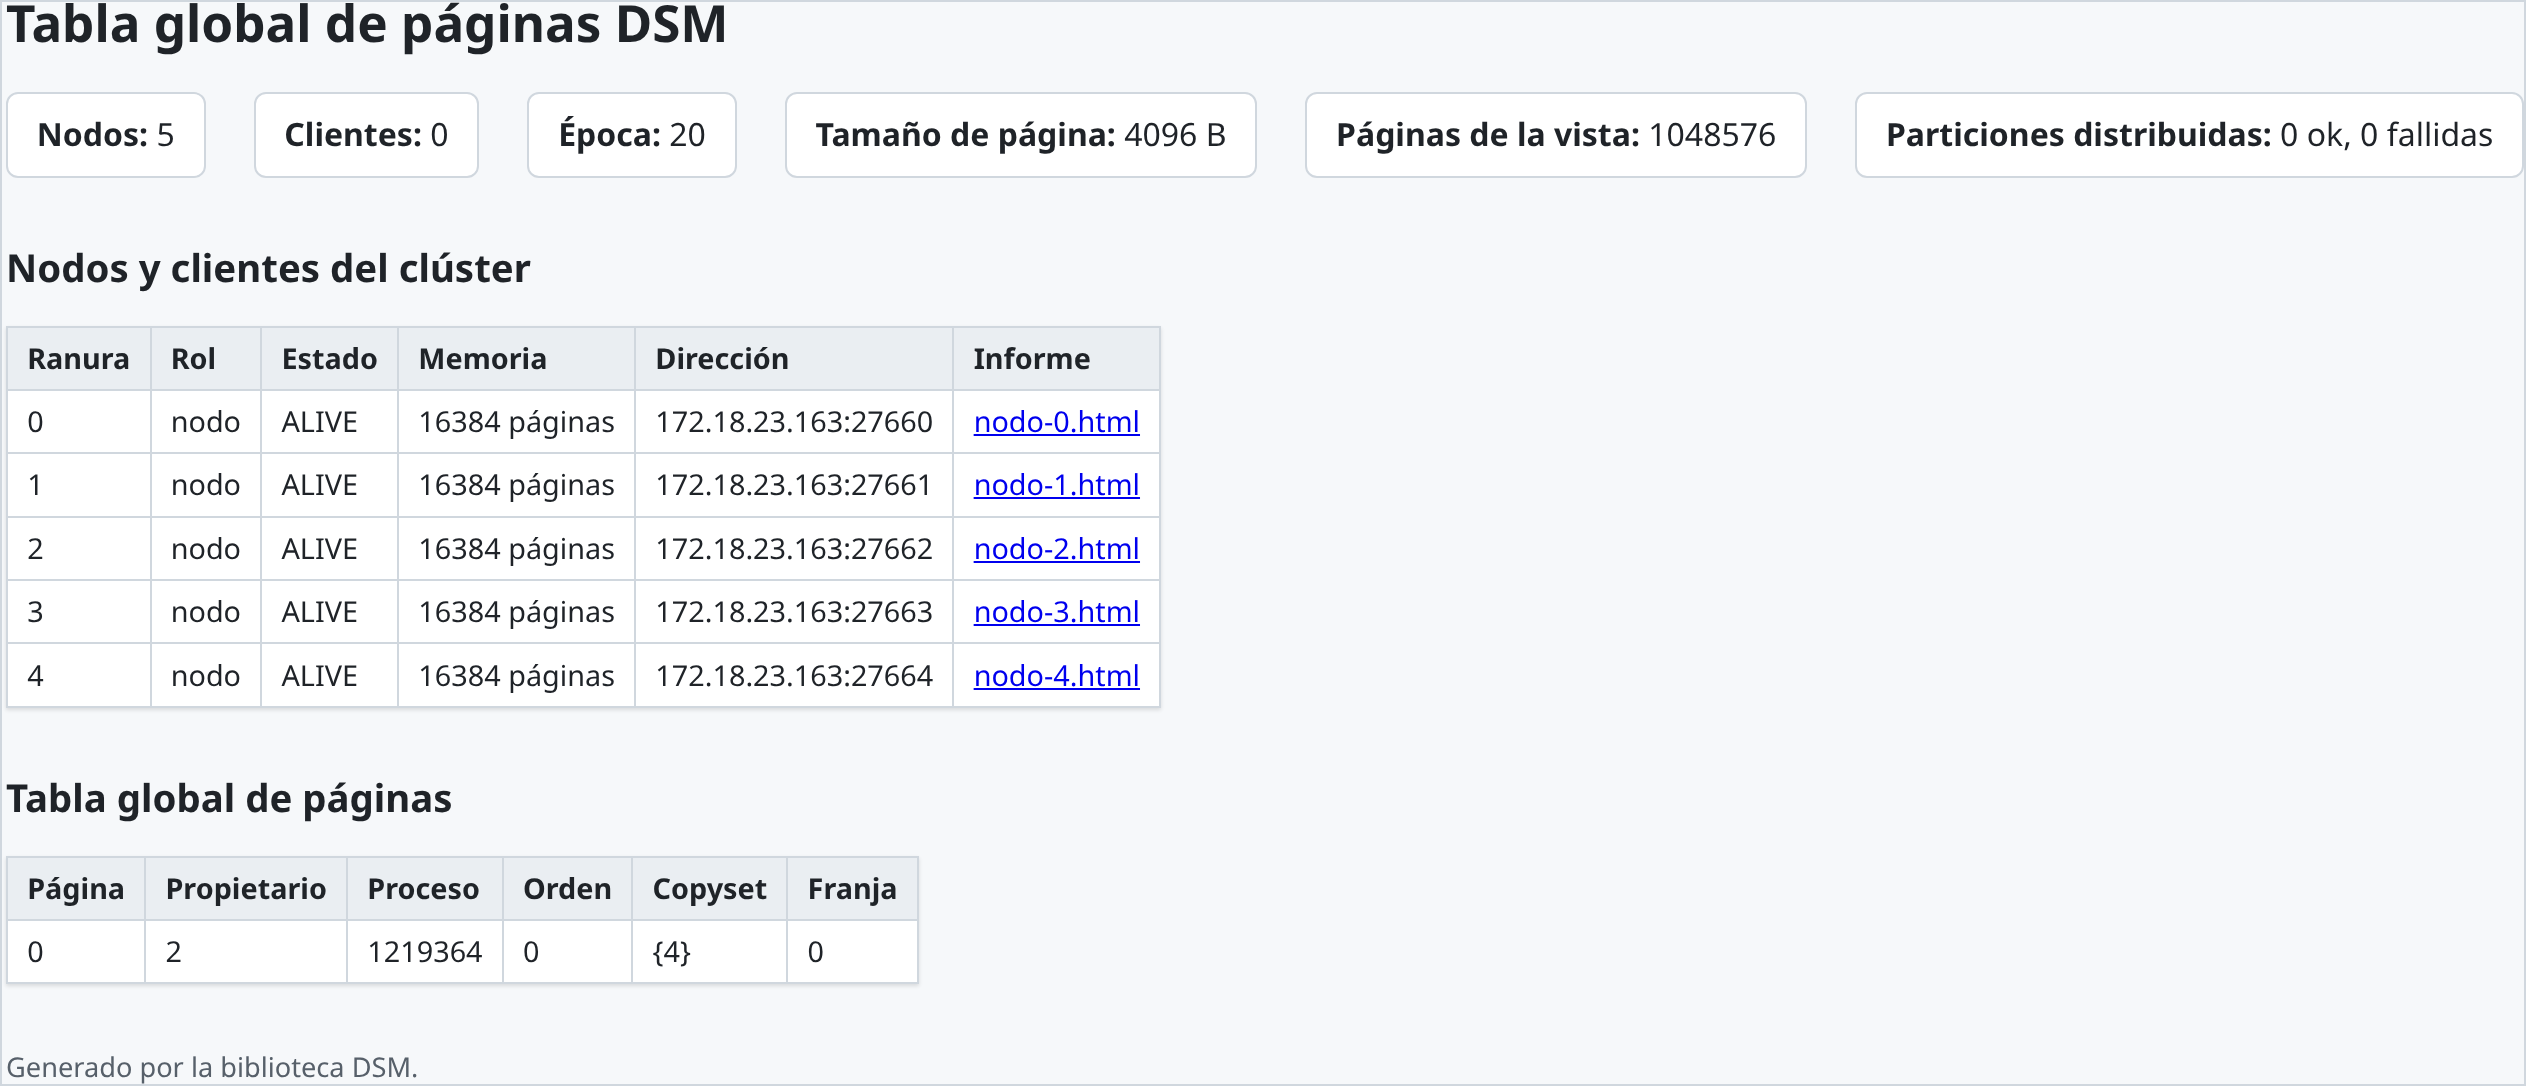
\includegraphics[width=\linewidth]{figuras/html-global.png}
\caption{Reporte global de páginas del clúster.}
\label{fig:html-global}
\end{figure}

La figura~\ref{fig:html-global} muestra un reporte global de una corrida local. Los recuadros superiores resumen cinco nodos, cero clientes, época 20, tamaño de página de 4096 B, 1\,048\,576 páginas de vista y cero particiones distribuidas correctas o fallidas. La lista de miembros tiene cinco filas, todas con rol \texttt{nodo}, estado \texttt{ALIVE}, 16\,384 páginas aportadas (64 MiB) y direcciones de la misma máquina en los puertos 27660 a 27664; cada fila enlaza su archivo \texttt{nodo-<ranura>.html}. La tabla global contiene una página materializada: la página 0, con propietario 2, proceso 1219364, orden 0, copyset \texttt{\{4\}} y franja 0.

Esa fila permite leer la diferencia entre custodio y copia. El propietario es la ranura que el anillo de dispersión asigna como home de la página; el copyset es el conjunto de ranuras que en ese momento tienen una copia válida en \texttt{S} o \texttt{M}. En la captura, el home es la ranura 2 y la única copia está en la ranura 4, de modo que el directorio de la página vive en 2 mientras el contenido modificado vive en 4. El proceso 1219364 es el PID que reservó el bloque, no el nodo que lo custodia; el orden 0 indica que la página es la primera de esa reserva, y la franja 0 que pertenece al primer grupo que usa el reporte. La tabla global no muestra el estado MSI porque cada nodo tiene el suyo para la misma página; esa información aparece en el archivo del nodo que conserva la copia.

\begin{figure}[H]
\centering
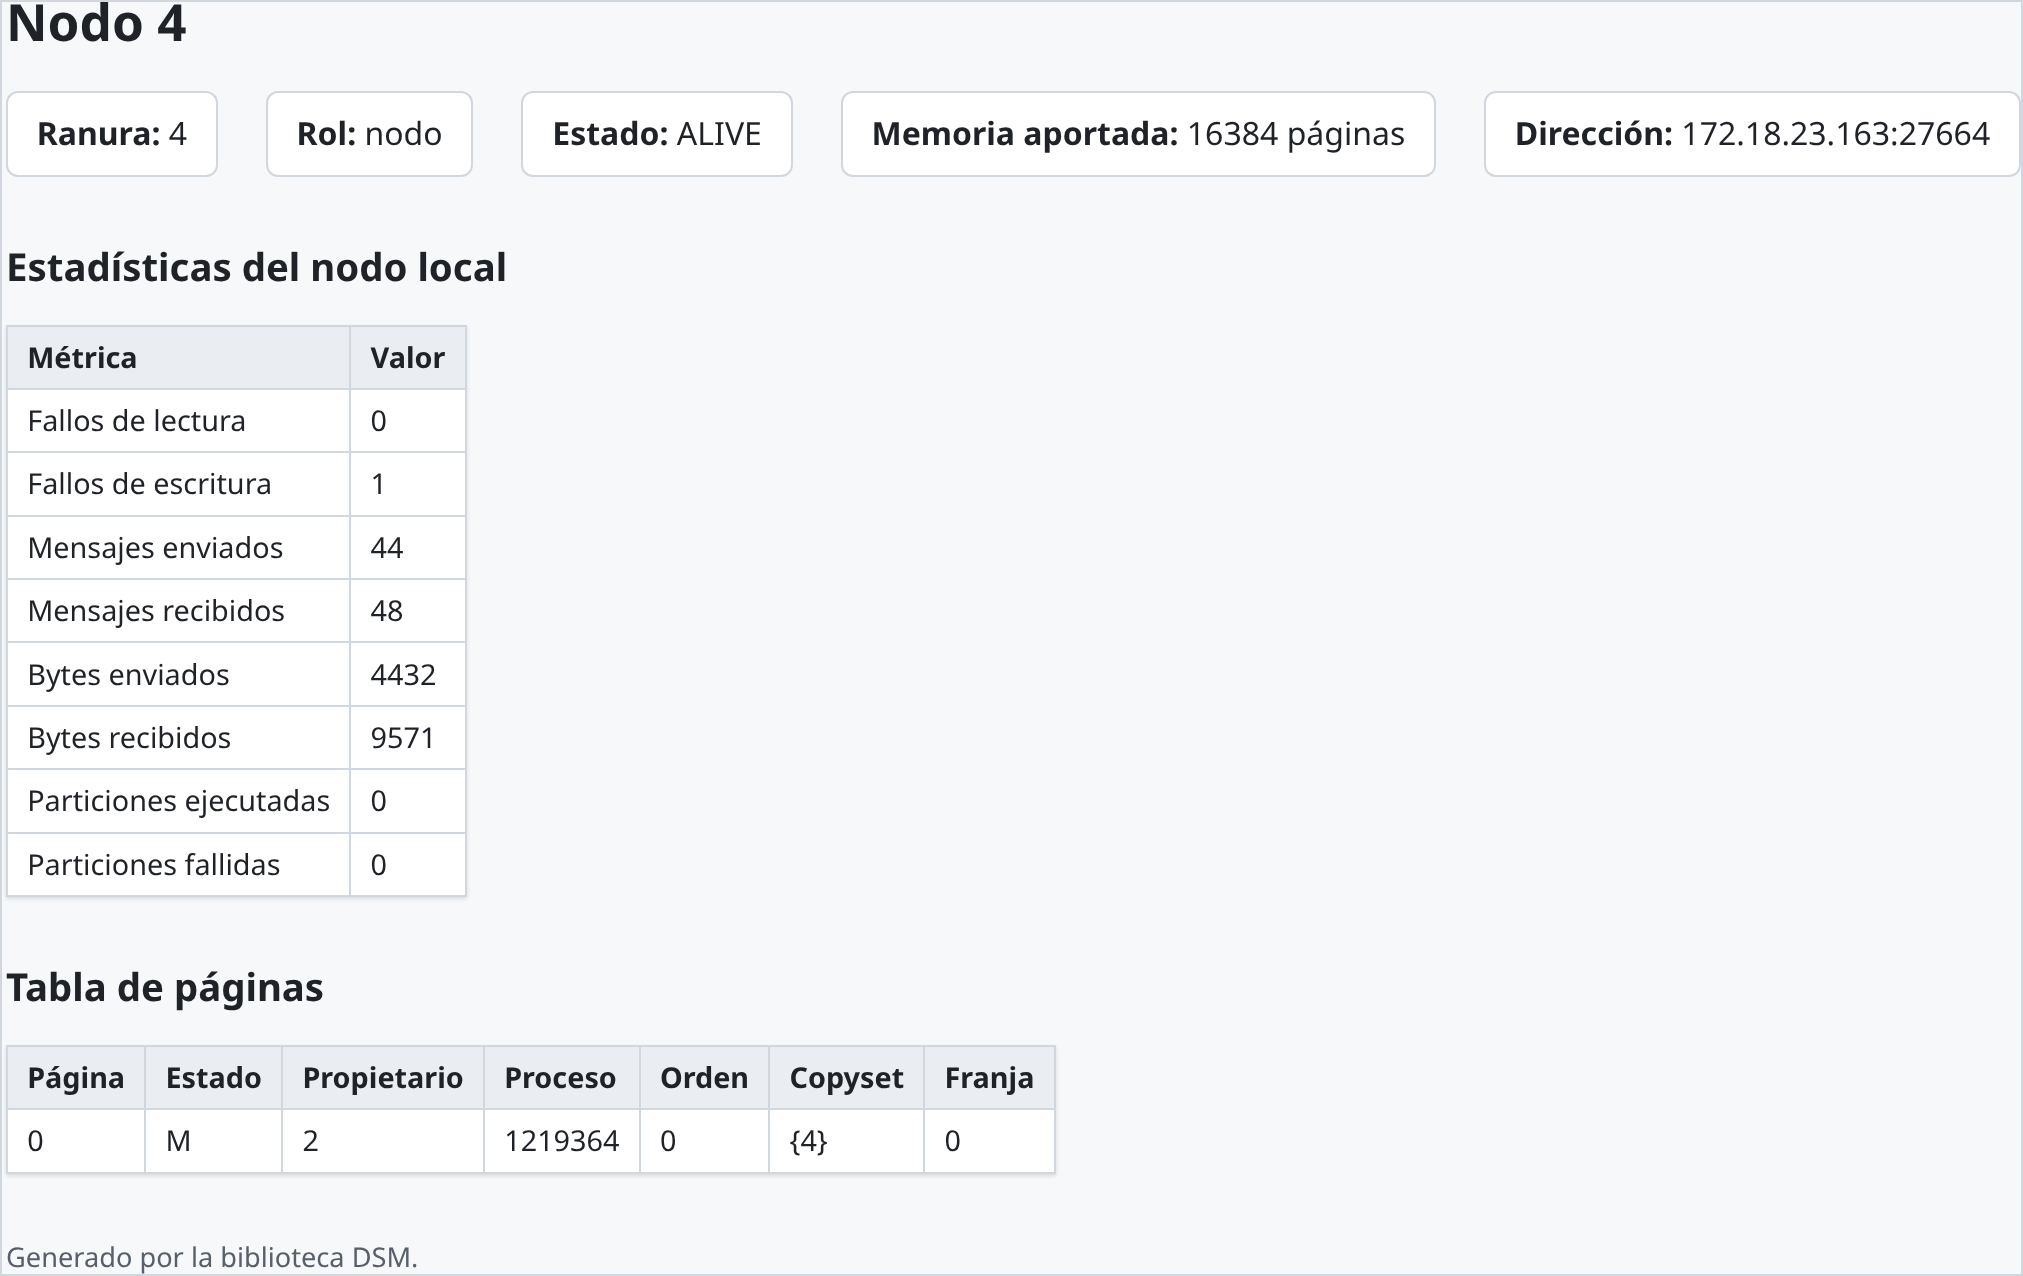
\includegraphics[width=\linewidth]{figuras/html-nodo.png}
\caption{Reporte de un nodo con una página en estado M.}
\label{fig:html-nodo}
\end{figure}

La figura~\ref{fig:html-nodo} corresponde al archivo del nodo 4 de la misma corrida. Los recuadros repiten ranura 4, rol \texttt{nodo}, estado \texttt{ALIVE}, 16\,384 páginas aportadas y la dirección 172.18.23.163:27664. Las estadísticas del nodo local registran 0 fallos de lectura, 1 fallo de escritura, 44 mensajes enviados, 48 recibidos, 4432 bytes enviados, 9571 bytes recibidos y 0 particiones ejecutadas o fallidas. La tabla de páginas tiene una fila: página 0, estado \texttt{M}, propietario 2, proceso 1219364, orden 0, copyset \texttt{\{4\}} y franja 0. El estado \texttt{M} confirma que la copia de la ranura 4 es la única válida y que está modificada; el propietario 2 sigue siendo el custodio del directorio.

Los nombres de las columnas se leen así. \textbf{Ranura} es la posición del miembro en la membresía, un número entre 0 y \texttt{MAX\_NODES}-1 que identifica al nodo en los mensajes y en el anillo. \textbf{Rol} distingue \texttt{nodo} de \texttt{cliente}: el primero aporta páginas y puede ser custodio, el segundo usa la vista sin aportar memoria. \textbf{Estado} en la lista de miembros vale \texttt{ALIVE}, \texttt{SUSPECT} o \texttt{DEAD}; en la tabla de páginas vale \texttt{M}, \texttt{S}, \texttt{I} o uno de los transitorios \texttt{IS\_PEND}, \texttt{IM\_PEND} y \texttt{SM\_PEND}. \textbf{Memoria} es la cantidad de páginas aportadas, que multiplicada por 4096 B da los MiB del nodo. \textbf{Dirección} es la IP y el puerto TCP de escucha. \textbf{Página} es el índice de la página dentro de la vista, no una dirección virtual: la dirección correspondiente es la base de la vista más \texttt{página} $\times$ 4096. \textbf{Propietario} es la ranura del custodio que asigna el anillo, no necesariamente la que tiene la copia. \textbf{Proceso} es el PID que reservó el bloque, o \texttt{-} si la página todavía no pertenece a ninguna reserva. \textbf{Orden} es el índice de la página dentro de esa reserva. \textbf{Copyset} es el conjunto de ranuras con copia válida en \texttt{S} o \texttt{M}; una página sin copia se muestra como \texttt{-}. \textbf{Franja} es el grupo que usa el reporte y, con redundancia activa, la paridad: en ese modo se calcula como página dividida entre $K$, con $K$ igual a los nodos vivos menos uno y acotado entre 2 y 8; sin redundancia se calcula como página dividida entre \texttt{CHUNK\_PAGES}, que vale 4 por omisión.

El reporte global y el de un nodo no son dos copias del mismo documento. El global omite el estado MSI y solo imprime las páginas que tienen al menos una copia, porque su objetivo es mostrar qué hay materializado en el clúster y quién lo tiene. El archivo por nodo imprime las páginas que ese nodo ve con estado distinto de \texttt{I}, incluye la columna \texttt{Estado} y añade las estadísticas locales cuando el archivo corresponde al nodo que genera el informe. Los clientes no tienen archivo propio, pero su tabla local se consulta para recuperar el PID y el orden reales de las páginas que conservan; por eso un copyset puede incluir una ranura de cliente aunque esa ranura no aparezca como nodo ni tenga archivo.

La generación tiene dos topes operativos. Recorre solo rangos de páginas materializadas, hasta 1024 rangos y 4096 filas, para que una vista de un millón de páginas con pocos datos no convierta el informe en una consulta sin fin. Las páginas en \texttt{I} no se escriben en el archivo por nodo, y las que no tienen copia no se escriben en el global. El recuadro \texttt{Páginas de la vista} indica el tamaño de la vista en páginas, no la cantidad de filas del informe; una vista de 1\,048\,576 páginas puede producir una tabla de una sola fila. El recuadro \texttt{Particiones distribuidas} cuenta las particiones que ejecutó el nodo que genera el informe, no la suma del clúster, porque se obtiene de \texttt{dsm\_stats} local.

\subsection{\texttt{demo}: coherencia, ejecución distribuida y paridad}\label{sec:demo}

\texttt{demo} reúne seis roles que se eligen con dos palabras en la línea de comandos. Los roles \texttt{dist coord} y \texttt{dist worker} ejercitan el registro de kernels y el reparto de particiones; \texttt{raid hold} y \texttt{raid produce} ejercitan la paridad y la reconstrucción; \texttt{msi a} y \texttt{msi b} ejercitan la coherencia entre dos procesos. Cada rol fija una etiqueta de nodo distinta para que varios procesos de la misma máquina no compartan identidad: \texttt{dist\_coord}, \texttt{dist\_worker}, \texttt{raid\_hold\_<pid>}, \texttt{raid\_producer\_<pid>}, \texttt{msi\_a\_<pid>} y \texttt{msi\_b\_<pid>}. Los roles que permanecen a la espera leen órdenes por la entrada estándar: \texttt{dist coord} acepta \texttt{LAUNCH <ranura>}, \texttt{raid hold} acepta \texttt{READ} y \texttt{READPAGE}, y \texttt{msi a} y \texttt{msi b} aceptan \texttt{READ} y \texttt{QUIT}; \texttt{dist worker} espera trabajo y \texttt{raid produce} recibe las páginas y los nodos como argumentos. Las respuestas empiezan por un marcador, y ese formato es el que usan las pruebas de extremo a extremo para controlar los procesos sin intervención manual.

\paragraph{\texttt{dist coord}.} Se une como nodo, reserva cuatro páginas (16 KiB), registra el kernel \texttt{0x44495354} y publica \texttt{COORD\_READY} con su ranura, la dirección virtual del bloque y el tamaño. Después lee líneas \texttt{LAUNCH <ranura>} y reparte ocho particiones de 1024 bytes entre su propia ranura y la ranura remota indicada. Los primeros 8 KiB del bloque contienen la fuente y los 8 KiB siguientes el destino; cada partición describe un rango de 1024 bytes en ambas regiones. El kernel aplica una XOR con la clave \texttt{0x5A}, de modo que el contenido de salida depende del código registrado en cada proceso y no de una simple copia. El coordinador lanza el trabajo, recoge los resultados, calcula el XOR de los CRC32 de las particiones de destino y llama a \texttt{dsm\_dist\_verify} y comprueba el patrón byte por byte. Al final imprime \texttt{DIST\_SLOTS}, una línea \texttt{DIST\_PART} por partición con ranura, origen, elementos y microsegundos, y \texttt{DIST PASS} o \texttt{DIST FAIL} con las claves \texttt{remote}, \texttt{total}, \texttt{verify} y \texttt{lectura}. La orden \texttt{QUIT} cierra el proceso.

\paragraph{\texttt{dist worker}.} Se une como nodo, registra el mismo kernel y publica \texttt{WORKER\_READY} con su ranura. No lanza trabajo: espera las órdenes \texttt{DIST\_RUN} que llegan por la red, ejecuta el kernel en el hilo trabajador que atendió el mensaje, calcula el CRC32 del rango de salida y responde \texttt{DIST\_DONE} con el estado, los elementos, el CRC, la duración y los fallos de lectura y escritura. El coordinador puede ejecutar sus propias particiones sin abrir una conexión contra su listener, así que el reparto por turno produce cuatro particiones locales y cuatro remotas cuando hay un trabajador. La orden \texttt{QUIT} lo cierra.

\paragraph{\texttt{raid hold}.} Se une como nodo y publica \texttt{HOLD\_READY} con su ranura. Después acepta \texttt{READPAGE 0x<va> <índice>} para comprobar una página o \texttt{READ 0x<va> <páginas>} para comprobar un rango completo. El patrón de cada página depende del índice y del desplazamiento: \texttt{(página} $\times$ 131 + \texttt{offset} $\times$ 17 + \texttt{0x5A) \& 0xFF}. Cada comprobación responde \texttt{PASS} o \texttt{FAIL}; la orden \texttt{QUIT} termina el proceso. Los procesos \texttt{hold} representan a los nodos que aportan memoria y permanecen vivos mientras el productor escribe y sincroniza.

\paragraph{\texttt{raid produce}.} Espera a que la membresía reúna la cantidad de nodos indicada, con un plazo de 30 s, reserva la cantidad de páginas pedida, escribe el mismo patrón página por página, llama a \texttt{dsm\_sync}, vuelve a leer el bloque y publica \texttt{RAID\_READY} con la dirección virtual, las páginas, su ranura, el resultado de la sincronización, el resultado de la lectura y los deltas de paridad locales. Si se ejecuta con \texttt{DSM\_NODE\_MODE=client}, no aporta memoria ni custodia páginas; las pruebas lo lanzan así para que los tres nodos \texttt{hold} sean los únicos custodios. El productor termina después de publicar la línea, de modo que ninguna copia local sobrevive; los \texttt{hold} pueden leer el bloque con la dirección publicada porque comparten la misma vista.

\paragraph{\texttt{msi a} y \texttt{msi b}.} El rol \texttt{a} reserva una página, la llena con el patrón \texttt{0xA0000000 + i} por cada palabra de 32 bits, publica \texttt{A\_READY PASS} con la dirección virtual y espera la orden \texttt{READ}. El rol \texttt{b} recibe esa dirección por argumento, se enlaza al DSM, lee la página y comprueba el patrón de A; después escribe el patrón \texttt{0xB0000000 + i} y publica \texttt{B\_AFTER\_WRITE PASS}. Cuando A recibe \texttt{READ}, vuelve a leer la página y comprueba el patrón de B. Si B obtuvo una copia modificada, A queda sin copia válida y su acceso produce un fallo de lectura que el despachador resuelve con el contenido nuevo. Los dos roles imprimen sus estadísticas antes y después de cada paso, y la orden \texttt{QUIT} los cierra.

La corrida de extremo a extremo confirma los tres mecanismos. La ejecución distribuida termina con \texttt{DIST PASS remote=4 total=8 verify=ok lectura=ok}, es decir, cuatro de las ocho particiones se ejecutaron en el trabajador remoto, las ocho se recogieron, el CRC agregado coincidió y la lectura del destino reprodujo el patrón. La prueba de paridad reconstruye 6 franjas y verifica 5 páginas después de la caída de un nodo. El flujo MSI entre dos procesos termina en \texttt{PASS}: B lee el patrón de A, lo modifica, A vuelve a fallar para leer el valor nuevo y las estadísticas muestran fallos de lectura y fallos atendidos. Estos resultados no se imprimen como un adorno: cada uno exige que el mecanismo haya hecho su trabajo, porque el patrón o el CRC fallarían si la página se hubiera servido mal.

\subsection{Interpretación de métricas y reportes}\label{sec:metricas}

Los contadores de \texttt{dsm\_stats} son acumulados del proceso desde \texttt{dsm\_init} hasta el momento de la consulta. \texttt{dsmctl stats} los suma recorriendo los miembros que responden, de modo que el agregado representa lo observado por esos procesos y no una verdad única del clúster. Un nodo que no contesta queda fuera de la suma, y un cliente que responde aporta sus contadores aunque no aporte memoria. El informe HTML, en cambio, usa las estadísticas del nodo que lo genera; por eso el recuadro de particiones distribuidas puede ser cero aunque otro nodo haya ejecutado trabajo.

Las fallas de lectura y escritura cuentan los accesos que dispararon \texttt{SIGSEGV} y que el despachador atendió. Una falla de lectura aparece cuando el proceso toca una página que no tiene o que fue invalidada; una de escritura aparece en la primera escritura sobre una página que estaba en \texttt{I} o en \texttt{S}. Al inicio de una aplicación las fallas crecen con las páginas que se materializan, y en régimen estable se estabilizan. Las páginas locales en \texttt{M}, \texttt{S} e \texttt{I} son una foto del momento: \texttt{M} indica copia exclusiva modificada, \texttt{S} copia de lectura compartida e \texttt{I} ausencia de copia válida. Un valor alto de \texttt{I} es normal, porque la vista tiene 1\,048\,576 páginas y una aplicación ocupa unas pocas; no significa que falten datos.

La latencia promedio por fallo es la suma acumulada de latencia dividida entre los fallos atendidos; incluye los fallos que terminaron en error, así que un valor alto puede reflejar reintentos y no solo distancia de red. Los mensajes enviados y recibidos, junto con los bytes, muestran el costo de coherencia: una aplicación con muchas fallas y pocos mensajes resolvió la mayor parte en el nodo local, mientras que una con muchos mensajes recurrió a custodios remotos. Las invalidaciones cuentan las copias locales que se retiraron por una escritura ajena; en el flujo MSI, la escritura de B sobre la página de A deja a A sin copia válida, por invalidación o por cambio de custodio, y explica que A vuelva a fallar al leer. Las respuestas descartadas por número de secuencia repetido o antiguo deben mantenerse bajas: un valor creciente indica retransmisiones o respuestas que llegan tarde, no trabajo útil.

Los deltas de paridad y las franjas reconstruidas pertenecen al modo con redundancia. Los deltas crecen con las escrituras que actualizan la paridad; las reconstrucciones solo aumentan cuando un nodo cae y una franja se recupera a partir de los datos supervivientes. En una corrida sana sin caídas, \texttt{stripe\_rebuilds} se queda en cero y los deltas reflejan la actividad de escritura. Los latidos perdidos cuentan transiciones a \texttt{SUSPECT} y \texttt{DEAD}, una por transición y no una por intervalo de retraso; un clúster estable muestra cero, como ocurre en el clúster local de cuatro nodos con 64 MiB por nodo, donde las cuatro ranuras registran \texttt{hb\_missed=0}. Las tareas distribuidas separan las particiones correctas de las fallidas; una partición fallida no aporta al CRC agregado, de modo que el XOR de verificación no depende del orden de llegada.

Las métricas de las aplicaciones se leen junto con su referencia. En \texttt{matmul 256 -{}-hilos 4} sobre el clúster local, el cálculo tarda 0.253 s, \texttt{dsm\_sync} 0.519 s y la referencia secuencial 0.048 s; el checksum coincide y no hay elementos distintos. La diferencia entre el cálculo y la referencia muestra el costo de resolver páginas durante el cálculo, y el tiempo de \texttt{dsm\_sync} muestra que la persistencia puede pesar más que la aritmética en una matriz pequeña. En el filtro de $640 \times 480$ con 30 cuadros, las 9000 fallas de escritura no bajan al aumentar los hilos porque son páginas, no operaciones: 6750 de entrada y 2250 de salida. En el juego de la vida de un solo nodo, las fallas de escritura tienden a igualar las páginas del par de tableros y los mensajes son cero; con varios nodos, los mensajes crecen y las fallas locales bajan, y esa relación es la que indica cuánto del tablero se resolvió por coherencia remota.

Los reportes HTML agregan una lectura que los contadores no dan. \texttt{Propietario} y \texttt{Copyset} permiten seguir una página hasta su custodio y sus copias; si el propietario no aparece en el copyset, la copia está en otro nodo, como en la figura~\ref{fig:html-global}, donde el home es 2 y la copia está en 4. \texttt{Estado} en el archivo del nodo confirma si esa copia es \texttt{M} o \texttt{S}; una página en \texttt{M} en un nodo y con el copyset reducido a esa ranura es el caso normal de una escritura exclusiva. \texttt{Memoria} indica lo que el nodo aporta, no lo que usa; un nodo con 16\,384 páginas aportadas puede tener una sola página materializada. \texttt{Páginas de la vista} es el tamaño lógico de la vista, no la cantidad de datos, y la tabla solo incluye páginas materializadas hasta los topes del informe. Con esas distinciones, el reporte sirve para auditar la colocación y la coherencia sin confundir capacidad con ocupación.

La interpretación correcta evita dos lecturas equivocadas. Un valor alto de \texttt{I} no es un error de coherencia: es la mayor parte de una vista que nadie tocó. Un valor alto de mensajes tampoco es un fallo: es el costo de resolver páginas en otros nodos, y se juzga junto con la latencia, las invalidaciones y el resultado de la verificación. La señal más fuerte de que el sistema hizo su trabajo es que la aplicación compare su salida con una referencia independiente y coincida; los contadores explican cuánto costó, no sustituyen esa comparación.

Una revisión breve del clúster sigue un orden que evita conclusiones apresuradas. \texttt{nodes} confirma la membresía, las ranuras y los roles; \texttt{stats} muestra si los contadores se mueven y si aparecen latidos perdidos, reconstrucciones o tareas fallidas; \texttt{pages} y \texttt{dir} ubican las páginas materializadas y sus copias; \texttt{alloc} relaciona esas páginas con la aplicación que las reservó; \texttt{html} deja el mismo estado en un documento que se puede conservar y comparar entre corridas; \texttt{config} verifica que el archivo cargado sea el que se cree. \texttt{demo} completa la revisión cuando hace falta provocar una transición que la carga normal no produce: una invalidación entre dos procesos, una partición ejecutada en otro nodo o una franja reconstruida tras una caída. El orden importa menos que la coherencia entre las fuentes: una página que la aplicación escribió y no aparece en ningún copyset, un contador que no corresponde al trabajo observado o un reporte sin la fila esperada son señales para revisar el mecanismo, no para ajustar el número.

\section{Validación experimental}\label{sec:validacion}

\subsection{Entorno y metodología}

La validación combina pruebas de extremo a extremo con corridas de las aplicaciones sobre la vista distribuida. El objetivo no es medir el rendimiento máximo de la máquina, sino comprobar que la coherencia, la reconstrucción y la ejecución remota producen resultados idénticos a una referencia secuencial cuando el clúster trabaja con memoria que ningún proceso contiene por completo. Cada escenario arranca procesos reales, con binarios compilados en el perfil que corresponde, y compara la salida del sistema contra un cálculo local independiente. Un escenario se declara exitoso solo si la comparación es exacta y, en los casos de tolerancia a fallos, si la operación afectada sigue disponible después de la baja.

Los cuatro perfiles de compilación se construyen con \texttt{make release}, \texttt{make debug}, \texttt{make asan} y \texttt{make tsan}. Los perfiles comparten \texttt{-Wall -Wextra -Wpedantic -Werror}, de modo que una advertencia impide generar el binario; las cuatro construcciones terminan sin avisos. Las pruebas de extremo a extremo usan los binarios de \texttt{debug} para conservar símbolos, mientras que las mediciones de las aplicaciones se hacen con \texttt{release}. Esa separación permite que un fallo de la prueba se depure con nombres y líneas, sin mezclar el costo de las comprobaciones de depuración con los tiempos que se reportan.

La prueba de extremo a extremo crea un archivo de configuración temporal con un identificador de clúster propio y un bloque de puertos libre, elige un grupo de descubrimiento distinto para no interferir con otras corridas y lanza los procesos con etiquetas únicas. La espera no se basa en dormir un tiempo fijo: el arnés lee la salida de cada proceso hasta encontrar un marcador, con un plazo amplio, y falla si el marcador no aparece o si el proceso termina antes. Los escenarios cubren el flujo MSI entre dos nodos, la ejecución distribuida entre un coordinador y un trabajador, y la caída de un custodio en un clúster con paridad. La orden \texttt{make test-e2e} ejecuta los tres y reporta un resultado por escenario.

\begin{figure}[H]
\centering
\begin{tikzpicture}[
    font=\footnotesize,
    box/.style={draw=borderblue, fill=softblue, thick, rounded corners, align=center, minimum width=2.9cm, minimum height=1.15cm},
    pc/.style={draw=bordergreen, fill=softgreen, thick, rounded corners, align=center, minimum width=3.0cm, minimum height=1.15cm},
    cli/.style={draw=borderorange, fill=softorange, thick, rounded corners, align=center, minimum width=3.0cm, minimum height=1.15cm},
    sw/.style={draw=purple!60!black, fill=softpurple, thick, rounded corners, align=center, minimum width=3.3cm, minimum height=1.15cm},
    link/.style={{Latex[length=2mm]}-{Latex[length=2mm]}, thick, draw=black!55},
    flow/.style={-{Latex[length=2mm]}, thick, draw=black!55},
    note/.style={font=\scriptsize, text=black!65, align=center}
]

\node[cli] (cli) at (0.8,0) {\textbf{Cliente}\\ \texttt{matmul}, \texttt{demo}\\ no aporta memoria};
\node[sw] (sw) at (4.9,0) {\textbf{Switch}\\ TCP 27600--27699\\ UDP \texttt{239.255.42.99}};

\node[pc] (p0) at (9.4,2.35) {\textbf{PC 0}\\ 256 MiB\\ ranura 0};
\node[pc] (p1) at (12.9,2.35) {\textbf{PC 1}\\ 128 MiB\\ ranura 1};
\node[pc] (p2) at (9.4,-2.35) {\textbf{PC 2}\\ 128 MiB\\ ranura 2};
\node[pc] (p3) at (12.9,-2.35) {\textbf{PC 3}\\ 128 MiB\\ ranura 3};

\draw[link] (cli.east) -- node[above, font=\scriptsize] {TCP} (sw.west);
\draw[link, dashed] (cli.south) to[bend right=12] node[below, font=\scriptsize] {anuncio UDP} (sw.south);

\draw[flow] (sw.east) -- (p0.west);
\draw[flow] (sw.east) -- (p1.west);
\draw[flow] (sw.east) -- (p2.west);
\draw[flow] (sw.east) -- (p3.west);

\node[note, above=0.28cm of sw] {configuración compartida\\ \texttt{NODE\_MEM} local};
\end{tikzpicture}
\caption{Montaje de validación del clúster físico con cuatro equipos y un cliente.}
\label{fig:montaje-validacion}
\end{figure}

La figura~\ref{fig:montaje-validacion} resume el montaje del clúster del laboratorio. Los cuatro equipos aportan memoria y se descubren por anuncios UDP en el mismo grupo; el cliente se conecta al clúster, usa la vista y no aporta páginas, de modo que ejecutar una aplicación no altera el tamaño ni la composición de la membresía. La configuración compartida debe coincidir en todos los procesos, mientras que \texttt{NODE\_MEM} puede variar y de hecho varía en el montaje físico, donde un equipo aporta el doble que los otros tres. Esa heterogeneidad es deliberada: comprueba que el anillo ponderado y el reparto de páginas aceptan capacidades distintas sin exigir la misma memoria en cada máquina.

Las corridas locales usan un solo equipo con varios procesos. El clúster local de referencia tiene cuatro nodos de 64 MiB, es decir, 256 MiB de capacidad agregada, con \texttt{REDUNDANCY=false}. La prueba de paridad usa tres nodos de 16 MiB con \texttt{REDUNDANCY=true} y un productor cliente, porque la redundancia exige al menos tres nodos vivos y deriva el número de datos por franja de la membresía. Las aplicaciones de medición se ejecutan como clientes, así que sus fallos de página se contabilizan en el proceso de la aplicación y no en los nodos que custodian las páginas, un detalle que conviene recordar al leer las estadísticas de \texttt{dsmctl}.

\subsection{Coherencia MSI entre dos nodos}

El primer escenario comprueba el camino completo de una página entre dos procesos. El proceso A se une al clúster, reserva una página, escribe un valor y publica la dirección virtual que recibió de \texttt{dsm\_alloc}. El proceso B se une después, recibe esa dirección y lee la página; la lectura falla porque B no tiene copia, el despachador consulta al custodio y la página llega con permiso de lectura. B escribe entonces un valor distinto, lo que obliga a invalidar o degradar la copia de A, y A vuelve a leer la página para confirmar que observa el valor escrito por B.

La prueba no exige que A reciba un mensaje de invalidación. Cuando B se une, el anillo puede cambiar y convertir a B en el nuevo custodio de la página; en ese caso A entrega su copia al nuevo custodio durante la sonda de traspaso y la suelta sin que haya una invalidación explícita que contar. La garantía observable es más fuerte que un contador: A debe volver a fallar para leer el valor de B, y la línea de estadísticas de A muestra \texttt{read\_faults} y \texttt{faults\_serviced} mayores que cero. El escenario termina con \texttt{PASS} y confirma que la coherencia no depende de que el custodio original permanezca en el mismo nodo.

El flujo ejercita las tres transiciones que sostienen el modelo. La lectura desde \texttt{I} instala una copia en \texttt{S}. La escritura desde \texttt{S} asciende a \texttt{M} después de invalidar las demás copias y esperar sus acuses. La lectura posterior desde una copia invalidada vuelve a \texttt{I} y repite la solicitud. Los estados transitorios aparecen en medio de cada una de esas transiciones, y el hecho de que el escenario termine sin bloqueos indica que el despachador y los trabajadores se coordinan sin que el manejador de la señal espere por la red.

\subsection{Multiplicación de matrices en el clúster}

La multiplicación de matrices es la prueba de carga con resultado numérico más directa. \texttt{matmul} reserva tres matrices de $N \times N$ elementos \texttt{double} con \texttt{dsm\_alloc}, llena A y B con un patrón determinista, reparte las filas de C entre los hilos y llama a \texttt{dsm\_sync} antes de verificar. La verificación calcula el checksum de C y compara cada elemento contra una referencia secuencial en memoria local, de modo que un solo valor distinto cambia el conteo de diferencias y el veredicto final.

La corrida de referencia usa $N=256$, cuatro hilos y el clúster local de cuatro nodos con 64 MiB por nodo. Cada matriz ocupa 0.5 MiB y las tres juntas 1.5 MiB, una carga pequeña frente a los 256 MiB aportados, pero suficiente para que las páginas se materialicen en custodios distintos y para que los hilos compitan por páginas compartidas. El resultado es un checksum de 41107839280, idéntico al de la referencia, con 0 de 65536 elementos distintos. La sincronización tarda 0.519 s, el cálculo 0.253 s y la referencia secuencial 0.048 s.

\begin{table}[H]
\centering
\small
\begin{tabularx}{\linewidth}{@{}r r r r r r r Y@{}}
\toprule
\textbf{N} & \textbf{Hilos} & \textbf{Nodos} & \textbf{Memoria} & \textbf{\texttt{dsm\_sync}} & \textbf{Cálculo} & \textbf{Distintos} & \textbf{Resultado} \\
\midrule
256 & 4 & 4 & 256 MiB & 0.519 s & 0.253 s & 0 de 65536 & Checksum correcto \\
256 & --- & 4 & 640 MiB & --- & --- & 0 de 65536 & Checksum verificado \\
\bottomrule
\end{tabularx}
\caption{Corridas de \texttt{matmul} sobre la vista distribuida. El guion indica un dato que la corrida no registra; la verificación del checksum no depende de esas marcas.}
\label{tab:corridas}
\end{table}

La tabla~\ref{tab:corridas} reúne las dos configuraciones medidas. La primera es homogénea y permite descomponer el tiempo; la segunda es el clúster físico heterogéneo de la subsección~\ref{sec:cluster-fisico}, donde la corrida confirma el checksum pero no conserva los tiempos parciales. La comparación relevante no es el tiempo absoluto, que depende de la máquina y de la carga del laboratorio, sino la igualdad del resultado y la proporción entre cálculo y sincronización. El cálculo sobre la vista queda por encima de la referencia secuencial porque cada primer acceso a una página dispara un fallo, una transición MSI y, cuando la página es remota, un intercambio por TCP. La sincronización es la partida dominante porque recorre las páginas modificadas y las persiste en el custodio, un costo que la referencia local no paga.

\subsection{Juego de la vida y filtro de video}

Las dos aplicaciones de prueba someten al sistema a patrones de acceso distintos. El filtro de video convierte un archivo RGB24 en escala de grises y escribe un byte por píxel; cada hilo toma un bloque contiguo de cuadros y la primera escritura sobre cada página de salida produce un fallo. El juego de la vida mantiene dos tableros y alterna entre ellos en cada generación; cada celda lee sus ocho vecinas, así que las filas del borde de un bloque tocan páginas que otro hilo puede estar modificando. El primer caso presiona la escritura densa y el segundo la lectura con fronteras entre bloques.

El filtro se ejecuta sobre el video versionado en \texttt{data/video\_128x96.rgb} con cuatro hilos. Una comprobación externa compara la salida byte por byte contra una conversión secuencial que aplica la misma fórmula de luminancia entera, de modo que una diferencia solo puede provenir de la coherencia y no de la convención de redondeo. La comparación recorre todos los píxeles y no encuentra discrepancias, y el programa informa los fallos de escritura atendidos junto con el rendimiento. La ejecución confirma que la vista compartida sirve para un flujo de datos que supera la memoria de un nodo cuando el clúster aporta páginas suficientes, sin que la aplicación tenga que copiar el archivo completo a memoria local.

El autómata se ejecuta sobre la fotografía versionada en \texttt{data/tablero\_192.gray}, con el tablero de 192 por 192 celdas, 30 generaciones y cuatro hilos. La opción \texttt{--verificar} repite la simulación en memoria normal con la misma semilla y la misma convención de borde toroidal, y compara el tablero final celda por celda. El programa informa una coincidencia exacta y, cuando hay una diferencia, la fila y la columna de la primera celda distinta. La prueba cubre un patrón de acceso con dependencias entre filas y columnas, distinto de la multiplicación de matrices, donde cada hilo escribe filas completas de C sin leer lo que escriben los demás.

Las dos aplicaciones usan la API como cualquier programa externo: \texttt{dsm\_init}, \texttt{dsm\_thread\_attach} en cada hilo que toca la vista, \texttt{dsm\_alloc} para las regiones y \texttt{dsm\_finalize} al terminar. Ninguna llama a \texttt{read} o \texttt{write} directamente sobre la vista, porque el kernel no puede resolver un fallo de página del DSM desde el contexto de una llamada al sistema; las dos copian a través de un búfer intermedio y dejan que el \texttt{memcpy} dispare el fallo que el despachador sí atiende. Esa restricción es parte del contrato de uso y aparece en las dos aplicaciones sin excepciones.

\subsection{Ejecución distribuida entre procesos}

El escenario distribuido arranca un coordinador y un trabajador como procesos independientes, cada uno con su propia conexión al clúster y su propia tabla de kernels. El coordinador registra el kernel de demostración, reserva un bloque en la vista y espera la orden \texttt{LAUNCH} con la ranura del trabajador. Al recibirla, divide el trabajo en ocho particiones y las reparte por turno entre los dos procesos; cuatro se ejecutan en el trabajador remoto y cuatro en el coordinador. El trabajador registra el mismo \texttt{kernel\_id} antes de recibir la orden, porque el registro es local y el coordinador no transporta código.

Cada partición se describe con direcciones de la vista, no con direcciones del montón de un proceso. El trabajador construye el descriptor, ejecuta el kernel en el hilo que atendió el mensaje y calcula el CRC32 del rango de salida. El resultado viaja en \texttt{DIST\_DONE} con el estado, la cantidad de elementos, el CRC, la duración y los contadores de fallos de lectura y escritura. El coordinador guarda cada resultado, rechaza un identificador repetido o fuera de rango y espera a que lleguen todas las particiones. La verificación compara el XOR de los CRC32 de las particiones con el valor esperado, de modo que el resultado agregado no depende del orden de llegada.

La corrida termina con \texttt{DIST PASS remote=4 total=8 verify=ok lectura=ok}. El campo \texttt{remote=4} confirma que la mitad de las particiones se ejecutó en el otro proceso; \texttt{total=8} confirma que no se perdió ninguna; \texttt{verify=ok} confirma que el CRC agregado coincide; \texttt{lectura=ok} confirma que el trabajador pudo leer el rango compartido que el coordinador había escrito. La prueba no se limita a comprobar que los mensajes llegaron: exige que el resultado numérico sea el correcto y que al menos una partición haya cruzado la red. Ese último requisito evita que un reparto que ejecuta todo localmente se declare exitoso.

El escenario también muestra que la ejecución distribuida se apoya en el mismo camino de fallos que las aplicaciones. Antes de invocar el kernel, el trabajador registra la pila alternativa del hilo, de modo que un acceso a una página que no tiene se resuelve por \texttt{SIGSEGV} y por el despachador, igual que en un hilo de aplicación. La partición puede leer y escribir la vista sin conocer si la página es local o remota. La diferencia está en el costo: una partición remota paga los fallos de página y los mensajes de coherencia, mientras que una local los resuelve contra su propio custodio cuando coincide con la ranura.

\subsection{Caída de nodo y reconstrucción con paridad}

La prueba de paridad arranca tres nodos con \texttt{REDUNDANCY=true}, un productor cliente y un bloque de 24 páginas. El productor escribe un patrón verificable, llama a \texttt{dsm\_sync} y termina; al cerrarse, sus copias locales desaparecen y el contenido queda en los custodios y en la paridad. La prueba consulta el directorio global para elegir una víctima y, sobre todo, para elegir páginas cuya franja conserve la compañera y la paridad. Una franja con dos páginas de datos en el mismo nodo pierde dos incógnitas cuando ese nodo cae, así que esas páginas no se pueden reconstruir y la prueba no las elige.

Después de la sincronización, la prueba derriba uno de los nodos custodios con \texttt{SIGKILL}. La detección de la baja no es instantánea: el detector espera los latidos perdidos, declara el nodo muerto, actualiza la membresía y encola la reconstrucción. El hilo de reconstrucción recorre las franjas afectadas, elige un líder entre las ranuras vivas y reúne la paridad y los datos supervivientes con \texttt{STRIPE\_READ}. Para cada franja calcula el bloque faltante por XOR y lo entrega al nuevo custodio. La prueba espera a que el contador de franjas reconstruidas deje de crecer antes de leer, porque una lectura que llega mientras la franja aún se reconstruye es terminal para el hilo.

La corrida reconstruye 6 franjas y verifica 5 páginas cuyo dato custodiaba el nodo caído. Las páginas se leen una por una desde un nodo superviviente y cada lectura debe devolver el patrón correcto; la primera lectura de cada página ejerce la reconstrucción. El resultado es \texttt{PASS}: la paridad conserva los datos tras la caída de un nodo. La diferencia entre las 6 franjas reconstruidas y las 5 páginas verificadas se explica porque algunas franjas contienen páginas que la prueba no elige para lectura, sea porque la página no pertenecía a la víctima o porque la franja tenía una segunda página de datos en el mismo nodo. La reconstrucción se ejecuta igual, pero la verificación se concentra en las páginas que la prueba puede leer con garantía.

El escenario deja explícito el alcance de la tolerancia. La paridad es de una pieza por franja, no de un nodo completo. Si dos páginas de datos de la misma franja viven en el mismo nodo, la caída de ese nodo elimina dos incógnitas y la reconstrucción no alcanza. El diseño evita que la paridad comparta nodo con un dato, pero no reparte los datos para que cada uno viva en una ranura distinta; esa colocación depende del anillo. La prueba elige solo las franjas recuperables y por eso puede afirmar que las páginas verificadas son correctas, sin ocultar que otras franjas del mismo bloque no habrían sobrevivido.

\subsection{Clúster físico de cuatro nodos}\label{sec:cluster-fisico}

El montaje físico reúne cuatro equipos del laboratorio conectados al mismo switch. Los equipos aportan 640 MiB en total: 256 MiB el primero y 128 MiB cada uno de los otros tres. La configuración compartida coincide en las once claves que entran en el hash, mientras que \texttt{NODE\_MEM} es distinto en cada archivo local. El descubrimiento por multicast encuentra a los pares sin una lista de equipos, y cada nodo toma el primer puerto libre del bloque asignado. La membresía se estabiliza con las cuatro ranuras y el reporte HTML se genera para los cuatro nodos.

La corrida de \texttt{matmul} con $N=256$ sobre el clúster físico verifica el checksum y reporta 0 de 65536 elementos distintos. El resultado es el mismo que en el clúster local, aunque la memoria aportada y la distribución de custodios son distintas. Esa igualdad es la evidencia más fuerte de que la coherencia no depende de una configuración particular: el mismo programa, el mismo archivo compartido y memorias desiguales producen el mismo valor. La corrida también confirma que el anillo ponderado asigna más páginas al equipo de 256 MiB y que el resto se reparte entre los tres equipos de 128 MiB sin que ninguno quede fuera.

El reporte HTML del clúster físico muestra las cuatro ranuras en estado \texttt{ALIVE}, con la memoria aportada por cada una y la dirección de escucha. La tabla global de páginas queda vacía porque la aplicación libera sus reservas al terminar, pero el archivo por nodo conserva la descripción de la vista y las estadísticas del proceso. La generación del reporte no requiere un servidor HTTP ni unirse al clúster: \texttt{dsmctl} abre una conexión efímera, pide la tabla y escribe los archivos en el sistema de archivos del nodo consultado.

La heterogeneidad del montaje también prueba el hash de configuración. Un archivo con distinto \texttt{NODE\_MEM} y el resto igual se acepta, porque la memoria local no forma parte del contrato compartido; un archivo con distinto \texttt{CLUSTER\_ID} o distinto tamaño de página se rechaza con \texttt{DSM\_ST\_CONFIG\_MISMATCH}. Esa separación es la que permite que un equipo con más memoria se una al mismo clúster sin obligar a los demás a declarar una capacidad que no tienen. La validación física confirma que la regla funciona en máquinas distintas y no solo en procesos de la misma máquina.

\subsection{Análisis de los resultados}

Las pruebas de corrección son consistentes entre sí. La coherencia MSI entre dos nodos termina en \texttt{PASS}; la multiplicación de matrices coincide en dos configuraciones distintas, con 0 de 65536 elementos diferentes; el filtro de video no encuentra discrepancias byte por byte; el autómata coincide celda por celda; la ejecución distribuida verifica el CRC agregado con cuatro particiones remotas de ocho; y la paridad reconstruye 6 franjas y permite leer 5 páginas después de la caída. Cada prueba compara contra una referencia independiente, no contra la salida del propio sistema, de modo que un error de coherencia que se repitiera en la referencia no podría pasar desapercibido.

Los tiempos de \texttt{matmul} muestran que la sincronización domina el costo. El cálculo sobre la vista tarda 0.253 s frente a 0.048 s de la referencia secuencial, y \texttt{dsm\_sync} tarda 0.519 s. La diferencia del cálculo se explica por los fallos de página y las transiciones MSI: cada página de A, B y C se materializa una vez, y las filas de C que comparten página entre hilos provocan invalidaciones y ascensos de permiso. La sincronización recorre las páginas modificadas y las persiste en el custodio; es el precio de que el contenido sobreviva a la caída del dueño, no un costo del algoritmo de multiplicación. La referencia secuencial no paga ninguna de las dos cosas porque trabaja en memoria local y no ofrece durabilidad distribuida.

La comparación entre el clúster local y el físico confirma que el resultado no depende de la homogeneidad. El clúster local tiene cuatro nodos iguales de 64 MiB; el físico tiene un nodo de 256 MiB y tres de 128 MiB. En ambos el checksum coincide y el conteo de diferencias es cero. La igualdad del valor no implica que la distribución de páginas sea la misma: el anillo ponderado asigna más vnodes al nodo de 256 MiB, y la ubicación de cada página cambia con la membresía. Lo que se conserva es la regla de coherencia, no una colocación fija.

La figura~\ref{fig:html-global} de la sección~\ref{sec:reportes-html} muestra el reporte global de una corrida local con cinco nodos de 64 MiB; uno de ellos ejecuta la aplicación de prueba. La tabla de nodos lista las cinco ranuras en estado \texttt{ALIVE}, cada una con 16\,384 páginas, y la tabla de páginas registra la página 0 en estado \texttt{M}, con el proceso que la materializó, su orden dentro del bloque y la franja de paridad. El reporte por nodo, en la figura~\ref{fig:html-nodo}, agrega las estadísticas locales y permite ver los fallos de lectura y escritura, los mensajes enviados y recibidos y las particiones distribuidas. Esa evidencia es la que hace observable el estado interno sin detener el clúster ni instrumentar la aplicación.

Las cifras de latidos perdidos completan el cuadro. En el clúster local de cuatro nodos, \texttt{hb\_missed} vale cero en las cuatro ranuras. El contador sube una sola vez por transición a \texttt{SUSPECT} y otra por transición a \texttt{DEAD}, no por cada intervalo de retraso, de modo que un cero significa que ningún par se declaró sospechoso ni muerto durante la corrida. Esa estabilidad es importante para interpretar los tiempos: si el detector hubiera marcado bajas falsas, la reconstrucción y el reajuste del anillo habrían introducido pausas que no pertenecen al algoritmo.

La validación tiene condiciones de operación que conviene explicitar. Las corridas se hacen en un laboratorio con los equipos conectados al mismo switch, sin particiones de red y con el modelo de fallos de parada: un nodo que falla deja de responder y no envía mensajes incorrectos. La prueba de paridad derriba un nodo con \texttt{SIGKILL}, que es el caso más limpio de ese modelo. Los tiempos dependen de la carga de las máquinas y del arranque del descubrimiento, así que se reportan como una medición puntual y no como un límite de rendimiento. La igualdad del checksum, en cambio, no depende de la carga y es la propiedad que sostiene las conclusiones.

\section{Conclusiones}\label{sec:conclusiones}

\subsection{Aportes del diseño}

El sistema demuestra que una memoria compartida distribuida puede ofrecer una interfaz de punteros normales sin renunciar a la coherencia ni a la tolerancia a fallos. La vista se proyecta sobre un \texttt{memfd} en una dirección común y se protege página a página con \texttt{mprotect}; la aplicación lee y escribe como si tuviera un bloque de memoria local, mientras el sistema resuelve cada fallo con el protocolo MSI. Esa decisión mantiene el modelo de programación simple y traslada la complejidad al núcleo, que es donde puede tratarse de forma uniforme para todas las aplicaciones.

El manejador de \texttt{SIGSEGV} es la pieza que hace posible la transparencia. El manejador no hace red, no toma locks y no reserva memoria: solo identifica la página, registra el fallo y duerme al hilo hasta que un despachador lo resuelve. Esa disciplina convierte una señal que normalmente termina el proceso en un mecanismo de demanda de páginas. El diseño separa el camino de la señal del camino de la red y evita que una espera de red dentro del manejador bloquee al proceso o introduzca dependencias circulares.

El directorio en el nodo custodio y el anillo de dispersión consistente eliminan la necesidad de un coordinador de propiedad. Cada página tiene un home que conoce sus copias, su dueño y su versión; el home se calcula de forma determinista a partir de la membresía y del UUID de cada nodo, ponderado por la memoria que aporta. Todos los nodos llegan al mismo resultado sin consultar a nadie, y cuando la membresía cambia solo se mueven las páginas de los tramos afectados. La combinación de directorio y anillo permite que la coherencia sobreviva a la caída de un custodio y que el contenido se transfiera al nuevo home con \texttt{PAGE\_MOVE}.

Los estados transitorios del protocolo MSI son otro aporte del diseño. Una transición no ocurre en el instante en que se solicita: la página pasa por \texttt{IS\_PEND}, \texttt{IM\_PEND} o \texttt{SM\_PEND} mientras la respuesta viaja por la red. Esos estados permiten describir la página durante la espera sin mantener un lock tomado, y los permisos de la vista reflejan lo que el nodo puede hacer en cada momento. El resultado es un protocolo que espera sin bloquear el resto del sistema y que puede agrupar solicitudes concurrentes sobre la misma página.

La redundancia con paridad completa el modelo con una garantía de disponibilidad. Las franjas agrupan $K$ páginas de datos y una de paridad, con la paridad en un custodio distinto de los datos. El delta de paridad se calcula al persistir, no en cada almacenamiento, y la reconstrucción por XOR recupera una pieza perdida a partir de las supervivientes. La validación confirma que la caída de un nodo no destruye el contenido de las franjas recuperables y que el sistema puede seguir leyendo después de la baja. La paridad no reemplaza la coherencia; la complementa para que una página no se pierda cuando su custodio desaparece.

La ejecución distribuida y los reportes HTML amplían el sistema más allá de la memoria compartida. Las particiones se describen con direcciones de la vista, los kernels se registran por proceso y los resultados se agregan con CRC32; los reportes convierten el estado interno en una tabla legible sin detener el clúster. Esa combinación de API, mensajes y observabilidad hace que el sistema pueda usarse como plataforma de aplicaciones y no solo como una demostración de coherencia.

\subsection{Lecciones de implementación}

La primera lección es que las restricciones del manejador de señales son parte del diseño y no un detalle de codificación. El manejador solo puede usar llamadas seguras para señales, y cualquier intento de hacer red, reservar memoria o tomar un mutex dentro de él introduce un riesgo de interbloqueo o de corrupción. La solución consiste en separar el registro del fallo de su resolución: el manejador deposita el fallo en una estructura por hilo y despierta a un despachador, que es un hilo normal y puede esperar. Esa separación es la que permite que el camino del fallo siempre termine, incluso cuando la red es lenta o un par no responde.

La segunda lección es que los trabajadores no deben esperar respuestas. Un trabajador que atiende una solicitud inicia la transacción, envía las invalidaciones necesarias y vuelve al pool; la respuesta final la cierra otro trabajador cuando llega el último acuse. Si los trabajadores esperaran, dos solicitudes cruzadas podrían formar un ciclo y bloquear el nodo. La regla de que solo los despachadores esperan, y de que lo hacen sobre respuestas que producen trabajadores que no esperan, mantiene el grafo de espera acíclico. Es una regla sencilla de enunciar y fácil de romper sin darse cuenta al agregar un camino nuevo.

El orden de \texttt{mprotect} también enseña una lección concreta. Al degradar una copia propia, el sistema cierra la escritura primero, copia el contenido después y solo entonces marca la página como compartida. Si copiara antes de cerrar la escritura, un hilo de la aplicación podría modificar la página entre la copia y el cambio de permiso, y el contenido entregado al solicitante no incluiría esa modificación. La secuencia parece un detalle menor, pero es la diferencia entre una copia consistente y una copia que puede quedar desactualizada en una ventana de pocos microsegundos.

La compuerta de \texttt{tseq} y el mapa de acuses resuelven dos problemas que no se ven en una prueba feliz. Una respuesta duplicada o reordenada puede llegar después de una versión más nueva; si se instalara, la página retrocedería. El contador de secuencia por página permite descartar la respuesta vieja antes de tocar el contenido. De forma parecida, una escritura que invalida varias copias necesita saber que todas llegaron, no solo la última; el mapa de acuses por transacción cuenta cada destinatario una vez y no se deja engañar por un duplicado. Esos dos mecanismos convierten el protocolo en algo que resiste la red real y no solo el orden ideal de una simulación.

La heterogeneidad de memoria obliga a separar lo compartido de lo local. El hash de configuración incluye las claves que deben coincidir y deja fuera \texttt{NODE\_MEM}, los plazos y los hilos. Esa separación permite que un equipo con más memoria se una al mismo clúster sin obligar a los demás a declarar una capacidad que no tienen. La validación física confirma que la regla funciona: cuatro equipos con 256, 128, 128 y 128 MiB comparten la misma vista y producen el mismo resultado. La configuración deja de ser un archivo idéntico para todos y pasa a ser un contrato común con parámetros locales.

Las pruebas con procesos reales descubren problemas que una prueba unitaria no ve. Los escenarios de extremo a extremo arrancan nodos, eligen puertos, esperan marcadores y comparan resultados; esa combinación ejercita el descubrimiento, la unión, la coherencia y el cierre en el mismo orden en que lo haría un usuario. La prueba de paridad, en particular, elige una víctima y páginas reconstruibles a partir del directorio real, de modo que no depende de una colocación supuesta. Esa forma de probar es más lenta que una simulación, pero es la que confirma que el sistema funciona cuando la red, los puertos y los procesos se comportan como en el laboratorio.

\subsection{Extensiones posibles}

Una ampliación deseable consiste en dar a la vista un almacenamiento persistente. El respaldo y la paridad viven en memoria; llevarlos a un archivo por nodo o a un dispositivo de memoria persistente permitiría conservar las páginas entre arranques y convertir \texttt{dsm\_sync} en un punto de recuperación. La misma estructura de marcos y versiones serviría para escribir un registro de cambios que reconstruya el estado después de una parada.

El reequilibrio dinámico de páginas es otra extensión natural. Cuando entra o sale un nodo, el anillo cambia y algunas páginas cambian de custodio; el sistema ya transfiere el contenido con \texttt{PAGE\_MOVE}. Un reequilibrio gradual permitiría mover las páginas en segundo plano, con un límite de transferencias por intervalo, para que una membresía grande no produzca una ráfaga que sature la red. El mismo mecanismo podría repartir las páginas de una franja entre nodos distintos y acercar la tolerancia de una pieza por franja a la tolerancia de un nodo completo.

La tolerancia a particiones de red exige un paso adicional sobre el modelo de fallos de parada. Un nodo que deja de responder no siempre está muerto: puede estar aislado y seguir ejecutando operaciones. Un esquema de quórum, arrendamientos o épocas con confirmación mutua permitiría distinguir una partición de una caída y evitar que dos mitades del clúster se declaren dueñas de la misma página. Esa extensión cambia las reglas de membresía y de directorio, pero conserva la idea de que cada página tiene un custodio y una versión.

Las transacciones multiescritor abren otra línea. La coherencia actual garantiza una página con un solo escritor o varios lectores, no una operación atómica sobre varias páginas. Una capa de transacciones con versiones, detección de conflictos y confirmación en dos fases permitiría actualizar estructuras enlazadas o índices sin que el programador tenga que construir su propio protocolo con \texttt{dsm\_lock}. La misma capa podría ofrecer memoria transaccional por software sobre la vista y reutilizar los cerrojos distribuidos como base.

El transporte también admite mejoras. TCP garantiza orden y entrega, pero agrega copias y cambios de contexto en cada página. Una implementación sobre RDMA o sobre sockets con memoria compartida reduciría la latencia de los fallos y liberaría CPU para el cálculo. El diseño de mensajes ya separa la cabecera de la carga y valida longitudes, de modo que un transporte nuevo podría conservar el mismo catálogo y cambiar solo el envío. La compresión de páginas o el uso de páginas grandes son variantes que se apoyan en la misma interfaz.

Un panel web con histórico de métricas complementaría los reportes actuales. El reporte HTML muestra una fotografía del estado; una serie temporal de fallos, latencia, tráfico y franjas reconstruidas permitiría ver tendencias y detectar un nodo que se degrada antes de que caiga. El panel podría leer las mismas consultas de \texttt{dsmctl} y guardar las muestras en un archivo o en una base ligera, sin agregar un servicio obligatorio al clúster.

Las aplicaciones de prueba también pueden crecer. Un procesador de imágenes por etapas, un motor de grafos, un compresor paralelo o una rutina de inferencia caben en el modelo de particiones descrito con direcciones de la vista. Cada una ejercita un patrón de acceso distinto y ayuda a medir el costo de la coherencia en cargas reales.


\appendix
\section{Catálogo de configuración}\label{app:config}

El archivo \texttt{dsm.conf} reúne las claves que gobiernan la identidad del clúster, la memoria, la red, los plazos y los grupos de hilos. Once de ellas forman el contrato compartido y se resumen en un CRC32 que viaja en el saludo: \texttt{CLUSTER\_ID}, \texttt{PAGE\_SIZE}, \texttt{BASE\_ADDR}, \texttt{VIEW\_SIZE}, \texttt{PORT\_MIN}, \texttt{PORT\_MAX}, \texttt{DISCOVERY\_GROUP}, \texttt{DISCOVERY\_PORT}, \texttt{VNODES\_PER\_MB}, \texttt{HOME\_SLACK} y \texttt{REDUNDANCY}. Las claves marcadas con asterisco en la tabla~\ref{tab:config-catalogo} pertenecen a ese grupo; las demás son locales y pueden variar entre equipos. \texttt{NODE\_MEM} es el caso más visible: cada PC declara la memoria que aporta y el hash la excluye para permitir clústeres heterogéneos.

{\footnotesize
\begin{xltabular}{\linewidth}{@{}l l l Y@{}}
\caption{Catálogo de claves de \texttt{dsm.conf}. El asterisco marca las claves que entran en el hash compartido.}\label{tab:config-catalogo}\\
\toprule
\textbf{Clave} & \textbf{Tipo} & \textbf{Valor típico} & \textbf{Efecto} \\
\midrule
\endfirsthead
\toprule
\textbf{Clave} & \textbf{Tipo} & \textbf{Valor típico} & \textbf{Efecto} \\
\midrule
\endhead
\midrule
\multicolumn{4}{r}{\footnotesize\textit{Continúa en la página siguiente}} \\
\endfoot
\bottomrule
\endlastfoot
\texttt{CLUSTER\_ID}$^{\ast}$ & hexadecimal & $0\text{x}534F3031$ & Identificador del clúster. Un valor distinto rechaza la unión con \texttt{DSM\_ST\_CONFIG\_MISMATCH}. \\
\texttt{PAGE\_SIZE}$^{\ast}$ & bytes & 4096 & Tamaño de la página virtual y de la unidad de coherencia; debe ser múltiplo de la página del sistema. \\
\texttt{BASE\_ADDR}$^{\ast}$ & hexadecimal & $0\text{x}200000000000$ & Dirección virtual común donde se proyecta la vista en todos los procesos. \\
\texttt{BASE\_ADDR\_TSAN} & hexadecimal & $0\text{x}4000000000$ & Dirección alternativa que usa la compilación con ThreadSanitizer para no chocar con su mapa. \\
\texttt{VIEW\_SIZE}$^{\ast}$ & bytes & 4294967296 & Extensión de la ventana virtual; no compromete memoria física hasta que se materializan páginas. \\
\texttt{MAX\_RUNTIME\_NODES} & entero & 256 & Tope de nodos admitidos en la membresía; no puede superar \texttt{MAX\_NODES}. \\
\texttt{VNODES\_PER\_MB}$^{\ast}$ & entero & 16 & Vnodes del anillo por MiB aportado; pondera la probabilidad de custodiar páginas. \\
\texttt{REDUNDANCY}$^{\ast}$ & booleano & \texttt{false} & Activa la paridad; con \texttt{true} la unión exige al menos tres nodos vivos y deriva $K$ de la membresía. \\
\texttt{CHUNK\_PAGES} & páginas & 4 & Agrupa páginas en la franja que muestran los reportes HTML; no cambia la colocación de datos. \\
\texttt{WAIT\_POOL\_ENTRIES} & entradas & 64 & Capacidad de particiones de un trabajo distribuido; un trabajo mayor devuelve \texttt{DSM\_ERR\_NO\_SPACE}. \\
\texttt{DIST\_TIMEOUT\_MS} & milisegundos & 5000 & Plazo por defecto de \texttt{dsm\_dist\_verify} cuando el trabajo aún no terminó. \\
\texttt{OUTPUT\_DIR} & ruta & \texttt{reports} & Directorio donde \texttt{dsm\_html\_report} escribe el archivo global y uno por nodo. \\
\texttt{NODE\_MEM} & bytes & 268435456 & Memoria física que aporta el proceso local; es local y puede variar entre equipos. \\
\texttt{PORT\_MIN}$^{\ast}$ & entero & 27600 & Primer puerto del bloque que el nodo recorre para tomar el primer puerto libre. \\
\texttt{PORT\_MAX}$^{\ast}$ & entero & 27699 & Último puerto del bloque; el rango debe estar libre y permitido por el cortafuegos. \\
\texttt{DISCOVERY\_GROUP}$^{\ast}$ & IPv4 & 239.255.42.99 & Grupo multicast donde cada nodo anuncia su UUID, IP, puerto, rol y páginas. \\
\texttt{DISCOVERY\_PORT}$^{\ast}$ & entero & 27699 & Puerto UDP del grupo de descubrimiento; el broadcast se usa como respaldo. \\
\texttt{CONNECT\_TIMEOUT\_MS} & milisegundos & 200 & Plazo de las conexiones no bloqueantes de sondeo. \\
\texttt{DISCOVERY\_TIMEOUT\_MS} & milisegundos & 300 & Espera máxima de una respuesta \texttt{WELCOME} tras el sondeo. \\
\texttt{SEND\_TIMEOUT\_MS} & milisegundos & 2000 & Plazo para emitir una trama completa antes de declarar fallo de enlace. \\
\texttt{REQUEST\_TIMEOUT\_MS} & milisegundos & 3000 & Espera de una respuesta asíncrona antes de reintentar la solicitud. \\
\texttt{REQUEST\_RETRIES} & entero & 3 & Cantidad de reenvíos antes de declarar inaccesible a un par. \\
\texttt{RECONNECT\_MIN\_MS} & milisegundos & 100 & Cota inferior del retardo exponencial para reabrir un enlace caído. \\
\texttt{RECONNECT\_MAX\_MS} & milisegundos & 2000 & Cota superior del retardo exponencial de reconexión. \\
\texttt{HB\_INTERVAL\_MS} & milisegundos & 500 & Intervalo entre latidos enviados a todos los pares. \\
\texttt{HB\_SUSPECT} & latidos & 3 & Latidos consecutivos perdidos que llevan una ranura a \texttt{SUSPECT}. \\
\texttt{HB\_DEAD} & latidos & 6 & Latidos consecutivos perdidos que declaran la ranura \texttt{DEAD}; debe superar a \texttt{HB\_SUSPECT}. \\
\texttt{WORKER\_THREADS} & hilos & 4 & Hilos que atienden solicitudes de red y ejecutan transacciones del protocolo. \\
\texttt{DISPATCHER\_THREADS} & hilos & 2 & Hilos que resuelven los fallos de página encolados por el manejador de \texttt{SIGSEGV}. \\
\texttt{PAGE\_LOCK\_STRIPES} & mutexes & 256 & Cantidad de cerrojos por franja que protegen el estado local de las páginas. \\
\texttt{HOME\_SLACK}$^{\ast}$ & factor & 1.25 & Margen sobre \texttt{NODE\_MEM} para el respaldo del custodio y los marcos de paridad. \\
\texttt{LOCK\_TIMEOUT\_MS} & milisegundos & 10000 & Plazo de \texttt{dsm\_lock} y \texttt{dsm\_barrier} antes de devolver \texttt{DSM\_ERR\_TIMEOUT}. \\
\texttt{WORKER\_QUEUE\_CAP} & mensajes & 4096 & Capacidad de la cola de solicitudes pendientes de despacho. \\
\texttt{DSM\_LOG\_LEVEL} & nivel & \texttt{INFO} & Nivel de detalle del registro: \texttt{ERROR}, \texttt{WARN}, \texttt{INFO}, \texttt{DEBUG} o \texttt{TRACE}. \\
\end{xltabular}
}

\section{Estructuras y cargas útiles}\label{app:protocolo}

Los mensajes viajan sobre TCP con una cabecera fija de 56 bytes seguida de una carga útil. La cabecera conserva el mismo formato en todas las versiones del protocolo y se serializa campo por campo en orden de red; el contenido de las páginas se transmite como bytes crudos. El CRC32 se calcula sobre la cabecera con su propio campo en cero y sobre la carga, de modo que una trama truncada o alterada se descarta antes de llegar a la lógica de coherencia. El catálogo completo y su agrupación por rangos aparece en la sección~\ref{sec:protocolo}.

Las estructuras que viajan por la red se serializan campo por campo y usan tipos de ancho fijo, de modo que su tamaño no depende del compilador. La tabla~\ref{tab:estructuras-protocolo} enumera las principales. La cabecera tiene 56 bytes en el cable y 64 en memoria por la alineación natural; el CRC32 ocupa el último campo y se calcula con ese campo en cero.

{\footnotesize
\begin{xltabular}{\linewidth}{@{}l l Y@{}}
\caption{Estructuras principales del protocolo y del estado local.}\label{tab:estructuras-protocolo}\\
\toprule
\textbf{Estructura} & \textbf{Tamaño} & \textbf{Contenido y uso} \\
\midrule
\endfirsthead
\toprule
\textbf{Estructura} & \textbf{Tamaño} & \textbf{Contenido y uso} \\
\midrule
\endhead
\bottomrule
\endlastfoot
\texttt{msg\_header\_t} & 56 B & \texttt{magic}, \texttt{cluster\_id}, \texttt{proto\_version}, \texttt{type}, \texttt{epoch}, \texttt{src\_slot}, \texttt{dst\_slot}, \texttt{req\_id}, \texttt{page\_id}, \texttt{tseq}, \texttt{data\_version}, \texttt{access}, \texttt{flags}, \texttt{status}, \texttt{payload\_len} y \texttt{crc32}. \\
\texttt{membership\_wire\_t} & 36 B & UUID, IP, puerto, ranura, estado, incarnation y páginas aportadas de un miembro. \\
\texttt{node\_info\_t} & 56 B & Registro local de membresía: UUID, incarnation, último latido, ranura, IP, páginas, vnodes, puerto, estado y latidos perdidos. \\
\texttt{dir\_entry\_t} & 72 B & Entrada del custodio: página, dueño, versión, \texttt{tseq}, marco, franja, cola de espera, transacción, estado, \texttt{busy} y \texttt{copyset} de 32 bytes. \\
\texttt{page\_local\_t} & 16 B & Estado MSI local, marcas \texttt{pend\_inval} y \texttt{pend\_down}, versión instalada, último \texttt{tseq} y cabeza de espera. \\
\texttt{stripe\_t} & 76 B & Identificador de franja, $K$, ranura de paridad, hasta ocho páginas de datos y sus custodios. \\
\texttt{alloc\_rec\_t} & 24 B & Identificador de reserva, primera página, cantidad, ranura, PID y relleno. \\
\texttt{discovery\_wire\_t} & 80 B & Anuncio UDP: UUID, clúster, hash compartido, IP, puerto, rol, páginas y versión. \\
\texttt{dist\_run\_wire\_t} & 48 B & Trabajo, kernel, partición, rango de la vista, cantidad de particiones y plazo. \\
\texttt{dist\_done\_wire\_t} & 44 B & Trabajo, partición, estado, elementos, CRC32, duración y fallos de lectura y escritura. \\
\texttt{dsm\_stats\_t} & variable & Contadores de fallos, mensajes, bytes, invalidaciones, latencia, paridad, ejecución distribuida y latidos. \\
\end{xltabular}
}

\section{Referencia de la API}\label{app:api}

Todas las funciones devuelven \texttt{dsm\_status\_t}: \texttt{DSM\_OK} vale cero y los valores negativos son errores. Cuando una función falla, no escribe en sus parámetros de salida. La tabla~\ref{tab:api-funciones} enumera las funciones públicas y los errores que cada una puede devolver; la tabla~\ref{tab:codigos-estado} describe los códigos. La referencia detallada de parámetros y estado de implementación está en \texttt{docs/API.md}.

{\footnotesize
\begin{xltabular}{\linewidth}{@{}l Y P{3.2cm}@{}}
\caption{Funciones públicas de la biblioteca DSM.}\label{tab:api-funciones}\\
\toprule
\textbf{Función} & \textbf{Propósito} & \textbf{Errores} \\
\midrule
\endfirsthead
\toprule
\textbf{Función} & \textbf{Propósito} & \textbf{Errores} \\
\midrule
\endhead
\midrule
\multicolumn{3}{r}{\footnotesize\textit{Continúa en la página siguiente}} \\
\endfoot
\bottomrule
\endlastfoot
\texttt{dsm\_init} & Carga la configuración, crea la vista y el alias, instala \texttt{SIGSEGV}, arranca hilos y se une al clúster. & \texttt{CONFIG}, \texttt{MEM}, \texttt{NET}, \texttt{PROTO}, \texttt{NO\_SPACE}, \texttt{INVALID} \\
\texttt{dsm\_finalize} & Anuncia \texttt{LEAVE}, detiene los hilos, cierra la red, restaura la señal y desmapea la vista. & \texttt{NOT\_INIT} \\
\texttt{dsm\_is\_initialized} & Indica si existe un contexto DSM activo en el proceso. & Ninguno \\
\texttt{dsm\_thread\_attach} & Asigna al hilo una pila alternativa y su ranura de fallo. & \texttt{NOT\_INIT}, \texttt{MEM} \\
\texttt{dsm\_thread\_detach} & Desactiva la pila alternativa y libera la ranura del hilo. & \texttt{NOT\_INIT} \\
\texttt{dsm\_alloc} & Reserva un bloque contiguo de páginas en la vista y devuelve su dirección. & \texttt{NOT\_INIT}, \texttt{INVALID}, \texttt{NO\_SPACE}, \texttt{BUSY}, \texttt{NET}, \texttt{PROTO} \\
\texttt{dsm\_free} & Devuelve un bloque al mapa global y deja sus páginas inválidas y en ceros. & \texttt{NOT\_INIT}, \texttt{INVALID}, \texttt{NO\_SPACE}, \texttt{BUSY}, \texttt{NET}, \texttt{PROTO} \\
\texttt{dsm\_sync} & Persiste las páginas en \texttt{M} en el respaldo de su custodio. & \texttt{NOT\_INIT}, \texttt{NET}, \texttt{TIMEOUT}, \texttt{MEM} \\
\texttt{dsm\_lock} & Adquiere un cerrojo distribuido y espera si el custodio lo tiene ocupado. & \texttt{NOT\_INIT}, \texttt{INVALID}, \texttt{BUSY}, \texttt{NO\_SPACE}, \texttt{TIMEOUT}, \texttt{NET} \\
\texttt{dsm\_unlock} & Libera el cerrojo que posee el hilo llamador. & \texttt{NOT\_INIT}, \texttt{INVALID}, \texttt{NET} \\
\texttt{dsm\_barrier} & Espera a que \texttt{n} participantes lleguen a la misma generación. & \texttt{NOT\_INIT}, \texttt{INVALID}, \texttt{NO\_SPACE}, \texttt{TIMEOUT}, \texttt{NET} \\
\texttt{dsm\_dist\_register} & Asocia un \texttt{kernel\_id} con una función y un argumento en la tabla local. & \texttt{NOT\_INIT}, \texttt{INVALID}, \texttt{NO\_SPACE} \\
\texttt{dsm\_dist\_launch} & Reparte las particiones por turno y envía \texttt{DIST\_RUN} a los trabajadores. & \texttt{NOT\_INIT}, \texttt{INVALID}, \texttt{NO\_SPACE}, \texttt{NET} \\
\texttt{dsm\_dist\_collect} & Copia los resultados disponibles de un trabajo. & \texttt{NOT\_INIT}, \texttt{INVALID}, \texttt{TIMEOUT}, \texttt{NET} \\
\texttt{dsm\_dist\_verify} & Espera el trabajo y compara el XOR de los CRC32 con el valor esperado. & \texttt{NOT\_INIT}, \texttt{INVALID}, \texttt{TIMEOUT}, \texttt{NET} \\
\texttt{dsm\_node\_id} & Escribe la ranura del nodo local. & \texttt{NOT\_INIT}, \texttt{INVALID} \\
\texttt{dsm\_node\_count} & Cuenta los nodos vivos que aportan memoria, sin incluir clientes. & \texttt{NOT\_INIT}, \texttt{INVALID} \\
\texttt{dsm\_global\_size} & Suma las páginas aportadas por los nodos vivos. & \texttt{NOT\_INIT}, \texttt{INVALID} \\
\texttt{dsm\_stats} & Copia los contadores acumulados y las páginas locales en \texttt{M}, \texttt{S} e \texttt{I}. & \texttt{NOT\_INIT}, \texttt{INVALID} \\
\texttt{dsm\_pages\_global} & Escribe la tabla de páginas materializadas con dueño, PID, orden, copyset y franja. & \texttt{NOT\_INIT}, \texttt{INVALID}, \texttt{NO\_SPACE}, \texttt{NET}, \texttt{PROTO} \\
\texttt{dsm\_html\_report} & Genera un archivo global y uno por nodo en el directorio indicado. & \texttt{NOT\_INIT}, \texttt{INVALID}, \texttt{NO\_SPACE}, \texttt{NET}, \texttt{PROTO} \\
\texttt{dsm\_strerror} & Devuelve la descripción estática de un código de estado. & Ninguno \\
\texttt{dsm\_debug\_dump\_fd} & Escribe ranura, época, dirección base, tamaño de vista y nodos activos en un descriptor. & \texttt{NOT\_INIT} \\
\end{xltabular}
}

{\footnotesize
\begin{xltabular}{\linewidth}{@{}r l Y@{}}
\caption{Códigos de estado del API.}\label{tab:codigos-estado}\\
\toprule
\textbf{Valor} & \textbf{Código} & \textbf{Significado} \\
\midrule
\endfirsthead
\toprule
\textbf{Valor} & \textbf{Código} & \textbf{Significado} \\
\midrule
\endhead
\bottomrule
\endlastfoot
0 & \texttt{DSM\_OK} & Operación completada. \\
-1 & \texttt{DSM\_ERR\_CONFIG} & Configuración inválida o hash compartido distinto. \\
-2 & \texttt{DSM\_ERR\_NOT\_INIT} & El subsistema no está inicializado. \\
-3 & \texttt{DSM\_ERR\_MEM} & Fallo de memoria, de hilos, de semáforos o de \texttt{memfd}/\texttt{mmap}. \\
-4 & \texttt{DSM\_ERR\_NET} & Sin puerto, conexión rechazada o enlace caído. \\
-5 & \texttt{DSM\_ERR\_TIMEOUT} & Plazo agotado en una espera. \\
-6 & \texttt{DSM\_ERR\_NO\_SPACE} & Sin páginas, ranuras o entradas de espera. \\
-7 & \texttt{DSM\_ERR\_INVALID} & Puntero nulo, tamaño cero o índice fuera de rango. \\
-8 & \texttt{DSM\_ERR\_NODE\_DOWN} & La ranura destino no pertenece a la membresía activa. \\
-9 & \texttt{DSM\_ERR\_BUSY} & Página o coordinador ocupado; la operación puede reintentarse. \\
-10 & \texttt{DSM\_ERR\_PROTO} & Cabecera, versión, tipo o CRC32 inválidos. \\
-11 & \texttt{DSM\_ERR\_INTR} & Llamada interrumpida por una señal; no la devuelve el API pública. \\
-12 & \texttt{DSM\_ERR\_AGAIN} & Recurso no disponible de inmediato; no la devuelve el API pública. \\
-13 & \texttt{DSM\_ERR\_NOT\_FOUND} & Sin pares durante el descubrimiento; \texttt{dsm\_init} la consume. \\
\end{xltabular}
}

\section{Evidencia de ejecución}\label{app:evidencia}

Los extractos siguientes provienen de corridas con binarios de \texttt{release} sobre el clúster local de cuatro nodos de 64 MiB. Las líneas se copian tal como las imprimen las herramientas, salvo los cortes de página y los espacios de alineación que el ancho del informe obliga a ajustar. Los identificadores UUID y las direcciones IP pertenecen a la corrida y cambian entre ejecuciones.

\subsection{Membresía}

\begin{lstlisting}[caption={Extracto de \texttt{dsmctl nodes} con la membresía del clúster local; se omite la columna UUID y se abrevian los encabezados para ajustar el ancho.}, label={lst:salida-nodes}]
Ranura  IP               Puerto  Rol   Estado  Aportadas  Libres  Latidos  Época
0       172.18.23.163    27600  nodo  ALIVE       16384   65536        0     15
1       172.18.23.163    27601  nodo  ALIVE       16384   65536        0     15
2       172.18.23.163    27602  nodo  ALIVE       16384   65536        0     15
3       172.18.23.163    27603  nodo  ALIVE       16384   65536        0     15
Nodos listados: 4
\end{lstlisting}

El listado muestra cuatro ranuras \texttt{ALIVE}, cada una con 16384 páginas, equivalentes a 64 MiB. El campo de latidos vale cero en las cuatro y el clúster reporta 65536 páginas libres, es decir, los 256 MiB agregados. La época es la misma para todos porque la membresía ya convergió cuando se hizo la consulta.

\subsection{Estadísticas agregadas}

\begin{lstlisting}[caption={Extracto de \texttt{dsmctl stats} después de una corrida de \texttt{matmul}.}, label={lst:salida-stats}]
Ranura  Rol   Fallos L  Fallos E  Mensajes  Deltas  Reconstruidas  Latidos perdidos
0       nodo         0         0      2260       0              0                 0
1       nodo         0         0      2538       0              0                 0
2       nodo         0         0      2341       0              0                 0
3       nodo         0         0      2358       0              0                 0
Nodos consultados: 4 de 4

Estadísticas agregadas del clúster
  Fallos de lectura        : 0
  Fallos de escritura      : 0
  Fallos totales           : 0
  Mensajes enviados        : 4750
  Mensajes recibidos       : 4747
  Bytes enviados           : 1900092, equivalente a 1.81 MiB
  Bytes recibidos          : 3448176, equivalente a 3.29 MiB
  Tareas distribuidas      : 0 correctas, 0 fallidas
  Deltas de paridad        : 0
  Franjas reconstruidas    : 0
  Respuestas descartadas   : 0
  Latidos perdidos         : 0
\end{lstlisting}

Los fallos de lectura y escritura de los nodos valen cero porque \texttt{matmul} se ejecuta como cliente: sus fallos se contabilizan en el proceso de la aplicación y no en los custodios. Los mensajes, en cambio, muestran actividad de red entre los cuatro nodos, que incluye los latidos y la atención del cliente. La última línea, \texttt{Latidos perdidos: 0}, es la que sostiene la afirmación de estabilidad de la membresía durante la corrida.

\subsection{Reporte HTML}

La figura~\ref{fig:html-nodo} de la sección~\ref{sec:reportes-html} muestra el formato del reporte por nodo en la corrida de cinco procesos. El reporte global de esa misma corrida describe la vista y la membresía. Los valores extraídos del archivo \texttt{global.html} son los siguientes:

\begin{lstlisting}[caption={Valores del reporte global \texttt{global.html} de la corrida local.}, label={lst:salida-html}]
Nodos: 5
Clientes: 0
Época: 20
Tamaño de página: 4096 B
Páginas de la vista: 1048576
Particiones distribuidas: 0 ok, 0 fallidas

Ranura  Rol   Estado  Memoria          Dirección
0       nodo  ALIVE   16384 páginas    172.18.23.163:27660
1       nodo  ALIVE   16384 páginas    172.18.23.163:27661
2       nodo  ALIVE   16384 páginas    172.18.23.163:27662
3       nodo  ALIVE   16384 páginas    172.18.23.163:27663
4       nodo  ALIVE   16384 páginas    172.18.23.163:27664
\end{lstlisting}

La vista declara 1048576 páginas, que corresponden a los 4 GiB de \texttt{VIEW\_SIZE}; la memoria aportada es mucho menor y se reparte entre los cinco nodos. El reporte por nodo de la figura~\ref{fig:html-nodo} agrega las estadísticas locales y la tabla de páginas materializadas, con el estado MSI de cada una.

\subsection{Multiplicación de matrices}

\begin{lstlisting}[caption={Salida de \texttt{matmul 256 --hilos 4} en el clúster local de cuatro nodos.}, label={lst:salida-matmul}]
Multiplicación de matrices sobre memoria DSM
Dimensiones: 256 x 256, elemento double
Hilos: 4
Matriz: 0.50 MiB; A, B y C: 1.50 MiB
Nodos activos: 4; memoria del clúster: 256.00 MiB
dsm_sync: OK (0.519 s)
Tiempo de cálculo: 0.253 s
Tiempo de referencia secuencial: 0.048 s
Checksum DSM: 41107839280.000000
Checksum referencia: 41107839280.000000
Diferencia máxima: 0.000000e+00
Elementos distintos: 0 de 65536
VERIFICACION: OK
\end{lstlisting}

Los tiempos corresponden a la corrida de la tabla~\ref{tab:corridas}. El checksum y el conteo de elementos distintos no cambian entre corridas, porque el cálculo es determinista y la verificación compara contra la referencia completa; los tiempos sí varían con la carga del equipo y con el momento en que se materializan las páginas.

\subsection{Pruebas de extremo a extremo}

\begin{lstlisting}[caption={Resultados de los tres escenarios de \texttt{make test-e2e}.}, label={lst:salida-e2e}]
=== Integración DSM: dos nodos y flujo MSI ===
PASS: flujo de página entre dos nodos

=== Integración DSM: ejecución distribuida entre dos procesos ===
DIST PASS remote=4 total=8 verify=ok lectura=ok
PASS: ejecución distribuida con dos procesos reales

=== Integración DSM: paridad, caída de un nodo y reconstrucción ===
Franjas reconstruidas: 6
Páginas reconstruidas y verificadas: 5
PASS: paridad conserva los datos tras la caída de un nodo
\end{lstlisting}

Los tres escenarios comparten el mismo arnés y se ejecutan con procesos reales. El primero confirma el flujo MSI entre dos nodos; el segundo exige que al menos una partición se ejecute en el otro proceso y que el CRC agregado coincida; el tercero derriba un custodio y verifica las páginas reconstruidas antes de declarar el éxito.


\end{document}
